\documentclass[twoside,11pt]{scrreprt}

\usepackage{graphicx}
\usepackage{amsfonts}
\usepackage{amsbsy}
\usepackage{verbatimfile}
% The next rawfonts package one is used in the ``datablad''.
% FIXME \usepackage[only,egtrm]{rawfonts}
% Handle sorting in reference list
\usepackage{citesort}
% Create an index table
\usepackage{makeidx}
% For html links in install chapter (install latex2html package to get
% this style)
% \usepackage{html}

\usepackage{color}
\usepackage{xcolor}
\usepackage{listings} 
 
\newcommand{\smallverbatimfile}[1]{{\footnotesize\verbatimfile{#1}}}

\def\reportnum{DTU}

\newcommand{\MCS}{{McStas}}
\newcommand{\version}{{2.0}}
\newcommand{\reldate}{{November, 2012}}
\newcommand{\Ombold}{\mbox{\boldmath $\Omega$}}

% enable index generation
\makeindex

\title{User and programmers guide\\ to the neutron ray-tracing package
 \MCS ,\\ version 2.0}
\author{P Willendrup, E Farhi, E Knudsen, U Filges, K Lefmann \\
Physics Department, \\
Technical University of Denmark, 2800 Kongens Lyngby, Denmark}
\date{\reldate \\[2\baselineskip]
\begin{center}

\includegraphics[width=4.5in]{figures/mcstas_logo}
\end{center}

\includegraphics[width=0.45cm]{figures/DTU_logo}
}

\begin{document}

\maketitle
%\input{risoe-rep-title}

\thispagestyle{empty}
% Emacs settings: -*-mode: latex; TeX-master: "manual.tex"; -*-

\begin{abstract}
The software package McXtrace is a tool for carrying out Monte Carlo
ray-tracing simulations of xray scattering beamlines with high
complexity and precision. The simulations can compute all aspects of the
performance of instruments and can thus be used to optimize the use of
existing equipment, design new instrumentation, and carry out virtual
experiments for e.g. training, experimental planning or data analysis. 
McXtrace is based is based on a unique design, inhereted from its sister McStas, 
where an automatic compilation process
translates high-level textual instrument descriptions into efficient
ANSI-C code. This design makes it simple to set up typical simulations
and also gives essentially unlimited freedom to handle more unusual
cases.


This report constitutes the reference manual for McXtrace, and,
together with the manual for the McXtrace components, it
contains full documentation of all aspects of the program. It covers
the various ways to compile and run simulations, a description of the
meta-language used to define simulations, 
and some example simulations performed with
the program.
\end{abstract}

\vskip\baselineskip\noindent
This report documents \MCX\ version \version, released \reldate
\vskip\baselineskip\noindent
The authors are:
\begin{quote}
\label{p:authors}
Erik B Knudsen \verb+<erkn@risoe.dtu.dk>+ \\
Materials Research Division, Ris{\o} DTU, Roskilde, Denmark 

Peter Kj\ae r Willendrup \verb+<peter.willendrup@risoe.dk>+ \\
Materials Research Division, Ris{\o} DTU, Roskilde, Denmark 

Emmanuel Farhi \verb+<farhi@ill.fr>+ \\
Institut Laue-Langevin, Grenoble, France 

Kim Lefmann \verb+<lefmann@fys.ku.dk>+ \\
Niels Bohr Institute, University of Copenhagen, Denmark 

\end{quote}
other people connected to the project:
\begin{quote}
Jana Baltser \verb+ <jana.baltser@fys.ku.dk>+ \\
Niels Bohr Institute, University of Copenhagen, Denmark 

Andrea Prodi \verb+ <aprodi@fys.ku.dk>+ \\
Niels Bohr Institute, University of Copenhagen, Denmark 

Manuel Sanchez del Rio \\
Computer Science Departement, ESRF, Grenbole, France

Claudio Ferrero \\
Computer Science Departement, ESRF, Grenbole, France
\end{quote}

%Peter Christiansen \verb+<pchristi@hep.lu.se>+\\
%Materials Research Department, Ris{\o} National Laboratory, Roskilde, Denmark\\
%Present address: University of Lund, Lund, Sweden\\
%Klaus Lieutenant \verb+<Klaus.Lieutenant@ife.no>+ \\
%Institut Laue-Langevin, Grenoble, France \\
%Present address: Institute for Energy Technology, Kjeller, Norway \\
%Kristian Nielsen \verb+<kristian-nielsen@mail.tele.dk>+ \\
%Materials Research Department, Ris{\o} National Laboratory, Roskilde, Denmark\\
%Presently associated with: MySQL AB, Sweden
%\end{quote}
%Front page illustration:\\[\baselineskip]
%Simulated scattering from a vanadium sample
%taking into account the secondary extinction. See
%section~\ref{s:vanadium-result}.

%\vfill
%\noindent ISBN 978--87--550--3679--6
%\par\noindent ISSN 0106--2840
%\par\noindent\hbox{}\hfill
%    Information Service Department $\cdot$ Ris{\o} DTU $\cdot$ \number\year
%    Information Service Department $\cdot$ Ris{\o} $\cdot$ \number\year
\par
\thispagestyle{empty}\clearpage





\tableofcontents
% Emacs settings: -*-mode: latex; TeX-master: "manual.tex"; -*-

\addcontentsline{toc}{chapter}{\protect\numberline{}{Preface and acknowledgements}}
\chapter*{Preface and acknowledgements}
This document contains information on the Monte Carlo neutron
ray-tracing program \MCS\ version \version, building on the initial
release in October 1998 of version 1.0 as presented in Ref.~\cite{nn_10_20}. The reader of this
document is supposed to have some knowledge of neutron scattering,
whereas only little knowledge about simulation techniques is
required. In a few places, we also assume familiarity with the
use of the C programming language and UNIX/Linux.

It is a pleasure to thank Prof.~Kurt N.~Clausen, PSI, for his continuous
support to this project and for having initiated \MCS\ in the first
place. Essential support has also been given by Prof.~Robert McGreevy, ISIS.
Apart from the authors of this manual, also Prof. Per-Olof \AA strand, NTNU Trondheim,
has contributed to the development of the \MCS\ system.
%Both he and our other collaborators, Henrik M.\ R\o nnow and Mark
%Hagen have made major contributions to the project.  Also the
%contributions from our test users, the students Asger Abrahamsen, Niels
%Bech Christensen, and Erik Lauridsen, are gratefully acknowledged; they
%gave us an excellent opportunity to pinpoint a vast amount of serious
%errors in the test version.  Useful comments to this document itself
%have been given by Bella Lake and Alan Tennant.
We have also benefited
from discussions with many other people in the neutron scattering
community, too numerous to mention here.

%Philipp Bernhardt contributed the two chopper components in
%sections~\ref{s:chopper} and~\ref{s:first_chopper}. Emmanuel Farhi
%contributed the components in sections~\ref{s:sourceoptimizer},
%\ref{s:monitornd}, and~\ref{s:monitoroptimizer}. We encourage other
%users to contribute components with manual entries for inclusion in
%future versions of \MCS.

In case of errors, questions, or suggestions,
%or other need for support should arise,
do not hesitate to
contact the authors at \verb+mcstas@risoe.dk+
or consult the \MCS\ home page~\cite{mcstas_webpage}.
A special bug/request reporting service is available \cite{mczilla_webpage}.

If you {\bf appreciate} this software, please subscribe to the \verb+neutron-mc@risoe.dk+ email list, send us a smiley message, and contribute to the package. We also encourage you to refer to this software when publishing results, with the following citations:
\begin{itemize}
\item{K. Lefmann and K. Nielsen, Neutron News {\bf 10/3}, 20, (1999).}
\item{P. Willendrup, E. Farhi and K. Lefmann, Physica B, {\bf 350} (2004) 735.}
\end{itemize}


\section*{\MCS\ \version\ contributors}
Several people outside the core developer team have been contributing
to \MCS\ \version:
\begin{itemize}
\item Mirror\_Elli.comp, Mirror\_para.comp,
  Focalisation\_mirrors.instr (Sylvain Desert, LLB)
\item PSI\_DMC.instr (L. Keller and U. Filges PSI / P. Willendrup, Ris\o\ DTU)
\end{itemize}
Thank you guys! This is what \MCS\ is all about!

Third party software included in \MCS\ are:
\begin{itemize}
\item perl Math::Amoeba from John A.R. Williams \verb+J.A.R.Williams@aston.ac.uk+.
\item perl Tk::Codetext from Hans Jeuken \verb+haje@toneel.demon.nl+.
\item scilab Plotlib from St\'ephane Mottelet \verb+mottelet@utc.fr+.
\item and optionally PGPLOT from Tim Pearson \verb+tjp@astro.caltech.edu+.
\end{itemize}
and special thanks to the following \MCS\ contributors:
\begin{itemize}
\item Christophe Taton from ENSIMAG/Grenoble for the MPI support
\item Reynald Arnerin from Universite J. Fourrier, Grenoble for the complex geometry support in samples
\end{itemize} 

The \MCS\ project has been supported by the European Union, initially
through the XENNI program and the RTD ``Cool Neutrons'' program in FP4,
In FP5, \MCS\ was supported strongly through the
``SCANS'' program.
Currently, in FP6, \MCS\ is supported through the Joint Research Activity
``MCNSI'' under the Integrated Infrastructure Initiative ``NMI3'', see
the home pages~\cite{mcnsi_webpage,nmi3_webpage}. \MCS\ is also
supported directly from the construction project for the ISIS second
target station (TS2), see~\cite{ts2_webpage}.


% Emacs settings: -*-mode: latex; TeX-master: "manual.tex"; -*-

\chapter{Introduction to \MCS}

Efficient design and optimization of neutron spectrometers are
formidable challenges, which are efficiently treated by Monte Carlo
simulation techniques.
When \MCS version 1.0 was released in October
1998, except for the NISP/MCLib program~\cite{nisp_webpage}, no existing package offered a general framework for the neutron
scattering community to tackle the problems currently faced at reactor and
spallation sources. The \MCS project was designed to provide such a framework.

\MCS %({\em Monte Carlo Simulations of Triple Axis Spectrometers\/})
is a fast and versatile software tool for neutron ray-tracing simulations.
It is based on a meta-language specially designed for neutron
simulation. Specifications are written in this language by users and
automatically translated into efficient simulation codes in ISO-C.
The present version supports both continuous and pulsed source instruments, and includes a library of standard
components with in total around 130 components. These enable to simulate all kinds of neutron scattering instruments (diffractometers, spectrometers, reflectometers, small-angle, back-scattering,...) for both continuous and pulsed sources.

The core \MCS package is written in ISO-C, with various tools based
on Perl and Python and is freely available for download
from the \MCS website~\cite{mcstas_webpage}. The package is actively
being developed and supported by DTU Physics,
Institut Laue Langevin (ILL), Paul Scherrer Institute and the Niels
Bohr Institute (NBI).
The system is well tested and
is supplied with several examples and with an extensive documentation.
Besides this manual, a separate component manual exists.

The release at hand \MCS \version is a major upgrade from the last
release, mainly because of our switch to the use of a Python user
interface layer. (The perl-based layer is still available, but we
recommend and encourage use of the new Python layer, since this is
where our efforts will go from this point.)

Porting your existing personal instrument files and
components should be trivial, but if you experience problems feel free
to contact  \verb+mcstas-users@mcstas.org+ or the authors.

%%%%%%%%%%%%%%%%%%%%%%%%%%%%%%%%%%%%%%%%%%%%%%%%%%%%%%%%%%%%%%%%%%%%%%%%%%%%%%%%
\section{Development of Monte Carlo neutron simulation}
The very early implementations of the method for neutron instruments used \emph{home-made} computer programs  (see e.g. papers by J.R.D. Copley, D.F.R. Mildner, J.M. Carpenter, J. Cook), more general packages have been designed, providing models for most parts of the simulations.
These present existing packages are: NISP \cite{NISP}, ResTrax
\cite{Restrax}, \MCS\cite{mcs_ppf,nn_10_20,mcstas_pb,mcs_ppf,mcstas_webpage},
Vitess \cite{Vitess,vitess_webpage}, IDEAS \cite{IDEAS} and IB (Instrument
Builder) \cite{IB_webpage}. Supplementing the Monte Carlo based
methods, various analytic phase-space simulation methods exist,
including Neutron Acceptance Diagram Shading (NADS) \cite{NADS_webpage}.
Their usage usually covers all types of neutron spectrometers, most of the time through a user-friendly graphical interface, without requiring programming skills.

The neutron ray-tracing Monte-Carlo method has been used widely for
{\em e.g.}\ guide studies \cite{Copley93,Farhi02,Schanzer04},
instrument optimization and design \cite{Zsigmond04,Lieutenant05}.
Most of the time, the conclusions and general behavior of such studies
may be obtained using the classical analytic approaches,
but accurate estimates for the flux, the resolutions,
and generally the optimum parameter set, benefit advantageously from MC methods.

Recently, the concept of virtual experiments, {\em i.e.}\ full simulations
of a complete neutron experiment, has been suggested as a major asset for neutron ray-tracing simulations. The goal is that
simulations should be of benefit to not only instrument builders, but also
to users for training, experiment planning, diagnostics, and data
analysis.

In the late 90'ies at Ris\o\ National Laboratory,
simulation tools were urgently needed,
not only to better utilize existing instruments
({\em e.g.} RITA-1 and RITA-2~\cite{cjp_73_697,pb_241_50,pb_283_343}),
but also to plan completely new instruments for new sources
({\em e.g.} the Spallation Neutron Source, SNS~\cite{sns_webpage}
and the planned European Spallation Source, ESS~\cite{ess_webpage}).
Writing programs in C or FORTRAN for
each of the different cases involves a huge effort, with debugging presenting
particularly difficult problems. A higher level tool specially designed
for simulating neutron instruments was needed. As there was
no existing simulation software that would fulfill our needs, the \MCS
project was initiated.
In addition, the ILL required an efficient and general simulation
package in order to achieve renewal of its instruments and guides.
A significant contribution to both the component library and the \MCS
kernel itself was early performed at the ILL and included in the package.
ILL later became a part of the core \MCS team.
Similarly, the PSI has applied \MCS extensively for instrument design
and upgrades, provided important component additions and contributed
several systematic comparative studies of the European instrument
Monte Carlo codes. Hence, PSI has also become a part of the core \MCS
team. 
Since year 2001 Ris\o\ was no longer a neutron source, and the authors
from that site have moved on to positions at University of Copenhagen
(NBI) and Technical University of Denmark (DTU Physics), hence these
two partners have joined the core \MCS team.
Finally, trough general emphasis on use of \MCS as a tool for
simulating the ESS instruments and virtual data, plus the partial
secondment of one DTU-based \MCS author, the ESS Data Management and
Software Centre (ESS DMSC) is now contributing to the projecte.

%%%%%%%%%%%%%%%%%%%%%%%%%%%%%%%%%%%%%%%%%%%%%%%%%%%%%%%%%%%%%%%%%%%%%%%%%%%%%%%%
\section{Scientific background}
What makes scientists happy? Probably collect good quality data, pushing the instruments to their limits, and fit that data to physical models.
Among available measurement techniques, neutron scattering provides a
large variety of spectrometers to probe structure and dynamics of all
kinds of materials.

Neutron scattering instruments are built as a series of neutron optics elements. Each of these elements modifies the beam characteristics (e.g. divergence, wavelength spread, spatial and time distributions) in a way which, for simple neutron beam configurations, may be modeled with analytic methods. This is valid for individual elements such as guides \cite{Leibnitz63,Mildner90}, choppers \cite{Lowde60,Copley03}, Fermi choppers \cite{Fermi47,Peters05}, velocity selectors \cite{Clark66}, monochromators \cite{Freund83,Sears97,Shirane02,Alianelli04}, and detectors \cite{Radeka74,Charpak89,Manzin04}. In the case of a limited number of optical elements, the so-called acceptance diagram theory \cite{Mildner90,Copley93,Cussen03} may be used, within which the neutron beam distributions are considered to be homogeneous, triangular or Gaussian.
However, real neutron instruments are constituted of a large number of optical elements, and this brings additional complexity by introducing strong correlations between neutron beam parameters like divergence and position - which is the basis of the acceptance diagram method - but also wavelength and time. The usual analytic methods, such as phase-space theory, then reach their limit of validity in the description of the resulting effects.

In order to cope with this difficulty, Monte Carlo (MC) methods (for a general review, see Ref.~\cite{James80}) may be applied to the simulation of neutron instruments.
The use of probability is common place in the description of microscopic physical processes. Integrating these events (absorption, scattering, reflection, ...) over the neutron trajectories
results in an estimation of measurable quantities characterizing the neutron instrument. Moreover, using variance reduction (importance sampling)
where possible, reduces the computation time and gives better accuracy.

Early implementations of the MC method for neutron instruments used \emph{home-made} computer programs  (see \cite{Copley86,Mildner77}) but, more recently, general packages have been designed, providing models for most optical components of neutron spectrometers.
The most widely-used packages are NISP \cite{NISP}, ResTrax \cite{Restrax}, \MCS \cite{mcs_ppf,nn_10_20,mcstas_webpage}, Vitess \cite{Vitess}, and IDEAS \cite{IDEAS}, which allow a wide range of neutron scattering instruments to be simulated.

The neutron ray-tracing Monte Carlo method has been used widely for
guide studies \cite{Copley93,Farhi02,Schanzer04}, instrument
optimization and design \cite{Zsigmond04,Lieutenant05}. Most of the
time, the conclusions and general behavior of such studies may be
obtained using the classical analytic approaches, but accurate
estimates for the flux, resolution and generally the optimum parameter
set, benefit considerably from MC methods, see Chapter~\ref{s:MCtechniques}.

Neutron instrument resolution (in $q$ and $E$) and flux are often limitations in the
experiments. This then motivates instrument responsibles to improve
the resolution, flux and overall efficiency at the spectrometer positions, and
even to design new machines. Using both analytic and numerical
methods, optimal configurations may be found.

But achieving a satisfactory experiment on the best neutron
spectrometer is not all. Once collected, the data analysis process
raises some questions concerning the signal: what is the background
signal? What proportion of coherent and incoherent scattering has
been measured? Is possible to identify clearly the purely elastic
(structure) contribution from the quasi-elastic and inelastic one
(dynamics)? What are the contributions from the sample geometry, the
container, the sample environment, and generally the instrument
itself? And last but not least, how does multiple scattering affect the
signal? Most of the time, the physicist will elude these questions
using rough approximations, or applying analytic corrections
\cite{Copley86}. Monte-Carlo techniques also provide means to evaluate
some of these quantities.

Technicalities of Monte-Carlo simulation
techniques are explained in detail in Chapter~\ref{s:MCtechniques}.

\subsection{The goals of \MCS}
\label{s:goals}

Initially, the \MCS project had four main objectives
that determined its design.

\paragraph{Correctness.}
\index{Bugs!hard to detect}
It is essential to minimize the potential for bugs in computer
simulations.  If a word processing program contains bugs, it will
produce bad-looking output or may even crash. This is a nuisance, but at
least you know that something is wrong. However, if a simulation
contains bugs it produces wrong results, and unless the results are far
off, you may not know about it! Complex simulations involve hundreds or
even thousands of lines of formulae, making debugging a major issue. Thus the
system should be designed from the start to help minimize the potential
for bugs to be introduced in the first place, and provide good tools for
testing to maximize the chances of finding existing bugs.
%
\paragraph{Flexibility.}
When you commit yourself to using a tool for an important project, you
need to know if the tool will satisfy not only your present, but also
your future requirements. The tool must not have fundamental limitations that
restrict its potential usage. Thus the \MCS systems needs to be
flexible enough to simulate different kinds of instruments
as well as many different kind of
optical components, and it must also be extensible so that future, as
yet unforeseen, needs can be satisfied.
%
\paragraph{Power.}
``\textit{Simple things should be simple; complex things should be possible}''.
New ideas should be easy to try out, and the time from thought to action
should be as short as possible. If you are faced with the prospect of programming for
two weeks before getting any results on a new idea, you will most likely drop
it. Ideally, if you have a good idea at lunch time, the simulation
should be running in the afternoon.
%
\paragraph{Efficiency.}
Monte Carlo simulations are computationally intensive, hardware capacities
are finite (albeit impressive), and humans are impatient. Thus the
system must assist in producing simulations that run as fast as
possible, without placing unreasonable burdens on the user in order to
achieve this.


%%%%%%%%%%%%%%%%%%%%%%%%%%%%%%%%%%%%%%%%%%%%%%%%%%%%%%%%%%%%%%%%%%%%%%%%%%%%%%%%
\section{The design of \MCS}
\label{s:design}
\index{McStas!design}
\index{Meta-language}

In order to meet these ambitious goals, it was decided that \MCS should
be based on its own \emph{meta-language} (also known as \emph{domain-specific language}), specially designed for
simulating neutron scattering instruments. Simulations are written in
this language by the user, and the \MCS compiler automatically
translates them into efficient simulation programs written in ISO-C.

In realizing the design of \MCS, the task was
separated into four conceptual layers, listed below and also detailed
in Figure \ref{fig:structure}
\begin{enumerate}
\item Graphical user interface and scripting layer, presentation of
  the calculations, graphical or otherwise. (aka. the tool layer).
\item Modeling of the overall instrument geometry, mainly consisting
  of the type and position of the individual components.
\item Modeling the physical processes of neutron scattering, \textit{i.e}.\
  the calculation of the fate of a neutron that passes through the
  individual components of the instrument (absorption, scattering at a
  particular angle, etc.)
\item Accurate calculation, using Monte Carlo techniques, of
  instrument properties such as resolution function from the result of
  ray-tracing of a large number of neutrons. This includes estimating
  the accuracy of the calculation.
\end{enumerate}

If you don't want to read this manual in full, go directly to the brief introduction in chapter \ref{s:brief}.

Though obviously interrelated, these four layers can be
treated independently, and this is reflected in the overall system
architecture of \MCS. The user will in many situations be
interested in knowing the details only in some of the layers. For
example, one user may merely look at some results prepared by others,
without worrying about the details of the calculation. Another user
may simulate a new instrument without having to reinvent the
code for simulating the individual components in the instrument. A third
user may write an intricate simulation of a complex component,
e.g.\ a detailed description of a rotating velocity selector,
and expect other users to easily
benefit from his/her work, and so on. \MCS attempts to make it
possible to work at any combination of layers in isolation by separating
the layers as much as possible in the design of the system and in
the meta-language in which simulations are written.

The usage of a special meta-language and an automatic compiler has
several advantages over writing a big monolithic program or a set of
library functions in C, FORTRAN, or another general-purpose programming
language.  The meta-language is more \textit{powerful}; specifications
are much simpler to write and easier to read when the syntax of the
specification language reflects the problem domain. For example, the
geometry of instruments would be much more complex if it were specified
in C code with static arrays and pointers. The compiler can also take
care of the low-level details of interfacing the various parts of the
specification with the underlying C implementation language and each
other. This way, users do not need to know about \MCS internals to
write new component or instrument definitions, and even if those
internals change in later versions of \MCS, existing definitions can be
used without modification.

The \MCS system also utilizes the meta-language to let the \MCS
compiler generate as much code as possible automatically, letting the
compiler handle some of the things that would otherwise be the task of
the user/programmer. \textit{Correctness} is improved by having a well-tested
compiler generate code that would otherwise need to be specially written
and debugged by the user for every instrument or component. \textit{Efficiency}
is also improved by letting the compiler optimize the generated code in
ways that would be time-consuming or difficult for humans to do. Furthermore, the
compiler can generate several different simulations from the same
specification, for example to optimize the simulations in different
ways, to generate a simulation that graphically displays neutron
trajectories, and possibly other things in the future that were not even
considered when the original instrument specification was written.

The design of \MCS makes it well suited for doing ``what if\ldots''
types of simulations. Once an instrument has been defined, questions
such as ``what if a slit was inserted'', ``what if a focusing
monochromator was used instead of a flat one'', ``what if the sample was
offset 2~mm from the center of the axis'' and so on are easy to answer. Within
minutes the instrument definition can be modified and a
new simulation program generated. It also makes it simple to debug new
components. A test instrument definition may be written
containing a neutron source, the component to be tested, and whatever
monitors are useful, and the component can be thoroughly tested before
being used in a complex simulation with many different components.

The \MCS system is based on ISO-C, making it both efficient and
portable. The meta-language allows the user to embed arbitrary C code in
the specifications. \textit{Flexibility} is thus ensured since the full
power of the C language is available if needed.


%%%%%%%%%%%%%%%%%%%%%%%%%%%%%%%%%%%%%%%%%%%%%%%%%%%%%%%%%%%%%%%%%%%%%%%%%%%%%%%%
\section{Overview}

The \MCS system documentation consists of the following major
parts:
\begin{itemize}
\item The complete listing of changes related to the version \MCS \version
is available in CHANGES document of the relevant download folder at
\url{http://download.mcstas.org/}. Bugs are reported and traced using
the \MCS GitHub issue system\cite{github_issue_webpage}. We will not
present here an extensive list of corrections, and we let the reader
refer to this bug reporting service for details. Only important
changes are indicated in the CHANGES document.
\item Chapter~\ref{s:MCtechniques} concerns Monte Carlo techniques
  and simulation strategies in general
\item Chapter~\ref{c:running} includes a brief introduction to the
  \MCS system
  (section~\ref{s:brief}) as well a section (\ref{s:running}) on running the compiler to produce
  simulations. Section~\ref{s:run-sim} explains how to run the generated
  simulations. Running \MCS on parallel computers require special
  attention and is discussed in section~\ref{s:run-mpi}. A number of front-end programs are used to run the
  simulations and to aid in the data collection and analysis of the
  results. These user interfaces are described in section~\ref{s:frontends}.
\item The \MCS meta-language is described in chapter~\ref{c:kernel}. This
  chapter also describes a set of library functions and definitions
  that aid in the writing of simulations. See
  appendix~\ref{c:kernelcalls} for more details.
\item The \MCS component library contains a collection of
  well-tested, as well as user contributed, beam components that can be used in simulations.
  The \MCS component library is documented in a separate manual
  and on the \MCS web-page~\cite{mcstas_webpage}, but a short overview of these
  components is given in chapter~\ref{c:components} of the Manual.
  %This
  %library is documented in detail in chapter~\ref{s:components}. Code
  %for the components can be found in appendix~\ref{compcode}.
% FIXME \item A collection of example instrument definitions is described in
% FIXME  chapter~\ref{c:instrument} of the Manual.%, with source code given in appendix~\ref{instcode}.

\end{itemize}

%In addition, some results from
%simulations with \MCS are described in
%appendix~\ref{testresults}.
As of this release of \MCS support for simulating neutron
polarization is strongly improved, e.g. by allowing nested magnetic
fields, tabulated magnetic fields in numerical input files and by close
to ``full'' support of polarization in all components. As this is the
first stable release with these new features, functionality is likely to change. To reflect this, the
documentation is still only available in the appendix of the Component manual. %~\ref{c:polarization}.
A list of library calls that may be used in component definitions
appears in appendix~\ref{c:kernelcalls}, and
an explanation of the \MCS terminology can be
found in appendix~\ref{s:terminology} of the Manual..
%Plans for future extensions are presented on the \MCS web-page~\cite{mcstas_webpage} as well as in section~\ref{s:future}.


%The \MCS package consists of four levels:
%\paragraph{The kernel.} Here are located some geometrical tools
%({\em e.g.} intersection between a line and various surfaces)
%and other elemental tools ({\em e.g.} creation and annihilation
%of a neutron). The kernel is maintained by the Ris\o\ group.

%\paragraph{The components.} Here resides the code for simulation
% of the individual spectrometer components
% (sources, detectors, samples, and optical elements).
% Components may have input parameters, like the angle of divergence of a
% collimator or the mosaicity of a monochromator crystal.
% Interested users are encouraged to modify existing components and to
% design new ones.
% A library of general and well documented components
% is being maintained by the Ris\o\ group.

%\paragraph{The instruments.} An instrument definition is written
% in the \MCS meta-language, which is a means of positioning
% components within an experimental geometry.
% Instruments may have inout parameters, like {\em e.g.}\ the three
% $(\omega,2\theta)$ pairs of a standard triple-axis spectrometer.
% For each specific instrument, a new instrument definition
% should be written. This will usually be done by the users,
% possibly in collaboration with the Ris\o\ group.

%\paragraph{The instrument control interface.}
% Here, the setting parameters of the
% instrument may be controlled in order to perform a simulation series.

% In the present version 1.0, the control interface
% consists of a very preliminary MATLAB program,
% but we expect soon to implement a simulation version of the
% Ris\o\ spectrometer control software TASCOM.
% By using the preprogrammed scans or the TASCOM programming features,
% the user will then be able easily to perform the desired simulations.
% Later, interfaces to other control software may be implemented.

%\paragraph{Data analysis and visualization}
% The output data is in the present version written as
% plain ASCII format, but will later be written in the TASCOM format,
% from where it may easily be converted into the general
% NeXus format\cite{NeXus}.
% This enables the user to choose between various analysis packages
% for the output side.
% Both ASCII and TASCOM files may be analysed and plotted through
% the Ris\o\ MATLAB package MVIEW/MFIT \cite{mview}.

% Emacs settings: -*-mode: latex; TeX-master: "manual.tex"; -*-

\chapter{New features in \MCX \version}
\label{c:changes}

\MCX is an ongoing evolving project with features being added frequently. While we strive to test it's features thoroughly, bugs
are inevitable. Bugs are generally reported using the user-mailing list: mcxtrace-users@mcxtrace.org and subsequently (after initial triage)
tracked using the \MCX\ Trac system \cite{mccode_trac_webpage}
(shared with its sister project \MCS). We will not present here an extensive
list of improvements and corrections, and we let the reader refer to this bug reporting service
for details. Only important changes are indicated here.
Of course, we can not guarantee that the software is bullet proof, but we do our best to correct bugs, when they are reported.\index{Bugs}

The main focus of the 1.2 release has been to improved stability and fixing bug, rather than new developments.

%\section{General}
%\label{s:new-features:general}
%\begin{itemize}
%\end{itemize}

\section{Kernel}
\label{s:new-features:kernel}
\index{Kernel}
An important update has been made to the approach of negative propagation lengths. Instead of inplicitly absorbing photons these are now generally restored.
In many cases the previous behaviour casued confusion and counter-inutitive operation, in particular regarding mutually exclusive monitors with the flag 
\texttt{restore\_xray} set.

\section{Run-time}
\label{s:new-features:run-time}
\index{Library!Run-time}
New intersection routines include \verb+ellipsoid_intersect+ and \verb+sphere_intersect+.

\section{Components and Library}
\label{s:new-features:components}
\index{Components} \index{Library!Components}
We here list the new and updated components (found in the \MCX \verb+lib+ directory)
which are detailed in the \textit{Component manual}. For an overview see the \textit{Component Overview} of the \textit{User Manual}(This Document).
%\subsection{General}
\subsection{New components}

\subsubsection*{Sources}
We have revised the following source models to make them work as conherently as possible while retaining the backwards compatibility.
\begin{description}
\item[Source\_pt] Point source.
\item[Source\_flat] Flat surface uniform source
\item[Source\_div] Flat surface uniform source with divergence distribution
\item[Source\_gaussian] Gaussian crossection source approximating a Bending Magnet
\end{description}
Furthermore we now also supply an experimental model of a bending magnet \texttt{Bending\_magnet}.
The following experimental components have been set up to facilitate interfacing with SPECTRA, Simplex, and GENESIS 1.3.
In general they take the output of the relevant external program to get a phase space distribution of photons from which McXtrace samples rays
to trace.
\begin{description}
  \item[Source\_genesis] Reads the output of a GENESIS 1.3 simulation. Useful for FEL-simulations. 
  \item[Source\_spectra] Reads the output of a SPECTRA simulation. Useful for Synchrotron simulations.
  \item[Source\_simplex] Reads the output of a Simplex simulation. Useful for FEL simulations.
\end{description}

\subsubsection*{Samples}
\begin{description}
  \item [Single\_crystal] Now has support for wavelength dependent absorption.
  \item [Molecule\_2state] Also includes absorption support.
  \item [Molecule\_2state] Option for supplying a q-parametrized scattering amplitude curve. This is for instance useful to add the effect of a well known solvent (e.g. Water) to a simulation.
  \item [SAXS] A whole set of SAXS-related samples is now available for various cases.
\end{description} 

\subsubsection*{Optics}
\begin{description}
  \item[Filter] Now has the option of taking any shape (through an .off or .ply-file.
  \item[Filter] Added a refraction-option. 
  \item[Multilayer\_elliptic] Elliptical multilayer mirror. This component now has the option of using a analytical kinematical approximation to compute refleticity as opposed to supplying a datafile. This is faster, but often less accurate.
  \item[Lens\_parab\_*] The lenses now behave in a similar manner wrt. parameter naming etc., also fixes to an error in the absorption computation. Note that the lens version will be merged in the next release (see the component manual).
  \item[Mirror\_elliptic] Elliptical shape mirror. Major geometry bug-fixes. Is scheduled to be merged with \texttt{Mirror\_curved}.
  \item[Mirror\_parabolic] Parabolic shape mirror. Major geometry bug-fixes. Is scheduled to be merged with \texttt{Mirror\_curved}.
  \item[Mirror\_curved] Cylindrical mirror. Fixed a bug which prevented its use as an azimuthal focusing mirror, with sideways incidence. 
  \item [Chopper\_simple] Optional random jitter was added.
  \item [Mask] A component that takes an image file as input, which is used to mask the beam. For instance to exmine linited resolution effects.
\end{description}

%\subsubsection*{Miscellaneous}
%\begin{description}
%  \item 
%----nothing has happened here leaving it in as a placeholder.
%\end{description}

\subsubsection*{Monitors}
\begin{description}
\item[TOF\_monitor] New Intensity vs. time of flight monitor. Useful for sime-resolved studies with pulsed sources.
\end{description}

\subsection{Example instruments}
The following beamline models have been added (in addition to unit test models that test specific components):
\begin{itemize}
  \item[XFEL\_SPB] A rough model of the SPB beamline at the Euorpean XFEL.
  \item[MAXII\_711] A model of the 711 powder diffraction beamline at Maxlab in Lund, Sweden.
  \item[MAXII\_811] Model of the 811 surface diffraction and EXAFS beamline at Maxlab in Lund, Sweden.
\end{itemize}

%\section{Documentation}
%\label{s:new-features:documentation}

\section{Tools, installation}
\label{s:new-features:tools}
\index{Tools}
\index{Installing}
\subsection{Selected Tool features}
\begin{itemize}
  \item standard FreeBSD port
    %  \item Support for per-user mcxtrace\_config.perl file, located in \verb+$HOME/.mcstas/+ . This folder is also the default
%     location of the 'host list' for use with MPI or gridding, simply name the file 'hosts'.
%  \item mxgui Save Configuration for saving chosen settings on the 'Configuration options' and 'Run dialogue'.
  \item Possibility to run MPI or grid simulations by default from mxgui.
%  \item When scanning parameters, mxrun now terminates with a relevant error message if one or more scan steps
%     failed (intensities explicitly set to 0 in those cases).
%  \item When running parameter optimisations, a logfile (default name is "mcoptim\_XXXX.dat" where XXXX is a
%     pseudo-random string) is created during the optimisation, updated at each optim step.
  \item We provide syntax-highlighting setup files for eamcs, vim and gedit editors.
\end{itemize}

\subsection{Warnings}
{\bfseries WARNING:} The 'dash' shell which is used as /bin/sh on some Linux system makes the 'Cancel' and 'Update' 
buttons fail in mxgui. Solutions are:
\begin{itemize}
  \item[a)] If your system is a Debian or Ubuntu, please dpkg-reconfigure dash and say 'no' to install dash as /bin/sh
  \item[b)] If you run another Linux with /bin/sh beeing dash, please install bash and manually change the /bin/sh link to point at bash.
\end{itemize}


% FIXME\chapter{Installing \MCS}
\label{installing}
\index{Environment variable!MCSTAS\_CC}
\index{Environment variable!MCSTAS\_CFLAGS}
\index{Environment variable!MCSTAS\_FORMAT}
\index{Testing the distribution}
\index{Installing}
The information in this chapter is also available as a separate
html/ps/pdf document in the \texttt{install\_docs/} folder of your
\MCS\ installation package.
\label{s:install}

\section{Getting McStas}
\label{s:obtain}
The \htmladdnormallink{McStas}{http://www.mcstas.org} package is
available in various distribution packages, from the project
website at
\htmladdnormallink{http://www.mcstas.org/download}{http://www.mcstas.org/download}.
\begin{itemize}
\item{\texttt{McStas-2.0-i686-Win32.exe}\\Windows self-extracting executable
    including essential support tools. - Refer to section
    \ref{s:win32_install}. }
\item{\texttt{McStas-2.0.dmg}\\Mac OS X disk image for PPC and Intel machines. Please follow
    the instructions in the README file in the disk image. }
\item{\texttt{mcstas-2.0-i386.deb}\\Binary Debian GNU/Linux packages for 32 bit Intel/AMD processors, currently built on Debian stable.
   Tested to work on Ubuntu and Debian systems.
 - Refer to section \ref{ss:deb_install}}
\item{\texttt{mcstas-2.0-amd64.deb}\\Binary Debian GNU/Linux packages for 64 bit Intel/AMD processors, currently built on Debian stable.
   Tested to work on Ubuntu and Debian systems.
 - Refer to section \ref{ss:deb_install}}
\item{\texttt{mcstas-2.0-i686-unknown-Linux.tar.gz}\\Binary package
  for Linux systems, currently built on Debian stable.
  Should work on most Linux setups.
 - Refer to section \ref{s:unix_install}}
\item{\texttt{mcstas-2.0-src.tar.gz}\\Source code package for
    building \htmladdnormallink{McStas}{http://www.mcstas.org} on
    (at least) Linux and Windows XP. This package should compile on
    most Unix platforms with an \texttt{ANSI-c} compiler. - Refer to section \ref{s:unix_install}}
\end{itemize}

\section{Licensing}
The conditions on the use of McStas can be read in the files
\verb+LICENSE+ and \verb+LICENSE.LIB+ in the distribution. Essentially,
McStas may be used and modified freely, and copies of the McStas source code
may be distributed to others.
New or modified component and instrument files may be shared by
the user community, and the core team will be happy to include user contributions in the package.

\section{Installation on windows}
\label{s:win32_install}
As of release 1.10 of McStas, the preferred way to install on
Microsoft Windows is using a self-extracting \texttt{.exe} file.

\noindent The archive includes all software needed to run McStas, including perl, a
c-compiler, PDL, PGPLOT, a vrml viewer.

\noindent Installation of all the provided support tools is needed to get a fully
functional McStas. (The option not to install the tools is included for people who want to
upgrade from a working, previous installation of McStas.)

\noindent The safe and fully tested configuration/installation is to install all
tools, leaving all installation defaults untouched. Specifically you
may experience problems if you install to non-standard locations.

\noindent Simply follow the guidance given by the installer, pressing 'next' all
the way.

\noindent To use grid and cluster computing, you will need an SSH client. McStas is configured to
use PuTTY.

\noindent We also recommend to install Gnuplot, Matlab or 
iFit (free Matlab replacement) from \\\htmladdnormallink{http://ifit.mccode.com/}{http://ifit.mccode.com/}, 
FreeWRL from \\\htmladdnormallink{http://freewrl.sourceforge.net/}{http://freewrl.sourceforge.net/}
or InstantPlayer from \\\htmladdnormallink{http://www.instantreality.org/}{http://www.instantreality.org/} 
or OctagePlayer from \\\htmladdnormallink{http://www.octaga.com/download\_octaga.html}{http://www.octaga.com/download_octaga.html}, 
and HDFView from \\\htmladdnormallink{http://www.hdfgroup.org/hdf-java-html/hdfview/}{http://www.hdfgroup.org/hdf-java-html/hdfview/}, 
prior to installing McStas.

\noindent For MPI (parallelisation) on Windows, we advice you to install MPICH2 from \htmladdnormallink{Argonne National Laboratory}{http://www-unix.mcs.anl.gov/mpi/mpich/} including development libraries before installing McStas. Also, your \verb+mpiexec.exe+ must be on the \verb+PATH+. You may have to customize the \verb+mpicc.bat+ script from the McStas distribution with the proper C compiler and MPI library path.

\noindent If you experience any problems, or have some questions or ideas
concerning McStas, please contact
\htmladdnormallink{pkwi@fysik.dtu.dk}{mailto:pkwi@fysik.dtu.dk}
or the McStas mailing list at \htmladdnormallink{mcstas-users@mcstas.org}{mailto:mcstas-users@mcstas.org}.


\section{Installation on Unix systems}
\label{s:unix_install}
Our current reference Unix class platform is
\htmladdnormallink{Ubuntu Linux}{http://www.ubuntu.com}, which is
based on \htmladdnormallink{Debian
  GNU/Linux}{http://www.debian.org}. Some testing is done on other
Unix variants, including \htmladdnormallink{Fedora
  Core}{http://fedora.redhat.com},
\htmladdnormallink{SuSE}{http://www.novell.com/products/suselinux/}
and \htmladdnormallink{FreeBSD}{http://www.freebsd.org}.
\ \\\ \\
 WARNING: The 'dash' shell which is used as /bin/sh on some Linux system (Including Ubuntu 8.04) makes the 'Cancel' and 'Update'
  buttons fail in mcgui. Possible solutions are:
\begin{itemize}
 \item If your system is a Debian or Ubuntu, please run the command
   \verb+dpkg-reconfigure dash+ and say 'no' to install dash as /bin/sh  (See section \ref{ss:deb_install})
 \item If your /bin/sh is dash, please install bash and manually change the /bin/sh link to point at bash.
\end{itemize}

\subsection{Debian class systems}
\label{ss:deb_install}
As of release 2.0, we provide a Debian binary package (32 bit package for Intel/AMD). We have tested that the
package works properly on Ubuntu and Debian systems. To install it, please
perform the following tasks:
\begin{enumerate}
\item{As root, issue the command \\\verb+apt-get install perl perl-tk gcc libc6-dev pdl bash+}
\item{Optionally, as root, issue the commands
\\\verb+apt-get install openssh-client openssh-server+
\\\verb+apt-get install mpi-default-bin mpi-default-dev+
to benefit from MPI and SSH grid parallelization}
\item{As root, issue the command \\\verb+dpkg-reconfigure dash+\\and
    say 'no' to install dash as /bin/sh.}
\item{Optionally, install FreeWRL from \verb+http://freewrl.sourceforge.net/download.html+, 
InstantPlayer from \\\htmladdnormallink{http://www.instantreality.org/}{http://www.instantreality.org/} 
or WhiteDune with \\\verb+apt-get install whitedune+.}
\item{To view OFF/PLY geometry files you may use Geomview or Meshlab, that can be installed with \\\verb+apt-get install geomview meshlab+.}
\item{If you have access to Matlab(R) or alternatively the free iFit replacement from \\\htmladdnormallink{http://ifit.mccode.com/}{http://ifit.mccode.com/}, install it prior to McStas, so that the configuration can detect it.}
\item{Download the packages from \verb+http://www.mcstas.org/download+}
\item{Double click the packages files (starting from the 'mcstas' one) or alternatively, as root, issue the command \\\verb+dpkg -i mcstas-2.x-amd64.deb+ (or \\\verb+dpkg -i mcstas-2.x-i386.deb+ on 32 bit systems). This later step may be replaced by a manual build from the Mctas tarball (see below)}
\item{Alternatively, as root, issue the commands \verb+sudo apt-add-repository 'deb http://packages.mccode.org/debian stable main ; apt-get update ; apt-get install mcstas-suite'+ :
\end{enumerate}
Updating your operating system to a new release \emph{may} in some cases require you to re-install McStas following the procedure above. 

\subsection{Other Linux/Unix systems}
To get a fully functional McStas installation on Unix systems, a few support
applications are required. Essentially, you will need a C compiler,
Perl and Perl-Tk, as well as a plotter such as Matlab, Gnuplot or
PGPLOT. In the installer package, we supply a method to install PGPLOT
and related perl modules - see step \ref{pg_install} below.

\noindent On Debian and Ubuntu systems, the
needed packages to install are \texttt{perl-tk, pdl, gcc,
  libc6-dev} \\(On Ubuntu you need to enable the 'universe' package
distribution in the file \\\verb+/etc/apt/sources.list+.)

\noindent We also recommend to install octaga VRML/X3D viewer such as
FreeWRL from \\\htmladdnormallink{http://freewrl.sourceforge.net/}{http://freewrl.sourceforge.net/} or 
InstantPlayer from \\\htmladdnormallink{http://www.instantreality.org/}{http://www.instantreality.org/}.

\noindent Additionally, MPICH, OpenMP (gcc-4.2 or icc or pgcc), openssh, Octave/Gnuplot, HDF and NeXus libraries may be installed, to enhance McStas clustering method and data formats.

\subsection{Configuration and installation}
McStas uses autoconf to detect the system configuration and creates the
proper Makefiles needed for compilation. On Unix-like systems, you
should be able to compile and/or install McStas using the following steps:
\begin{enumerate}
\item{Unpack the sources to somewhere convenient and change to the
    source directory:\\
  \texttt{gunzip -c <package>.tar.gz | tar xf -}\\
  \texttt{cd mcstas-2.0/}}
\item{Configure McStas:\\
  \texttt{./configure} or \texttt{./configure --with-nexus --with-cc=gcc-4.2}}
\item{Build McStas (only in case of the \verb+mcstas-2.0-src.tar.gz+ package):\\
  \texttt{make}}
\item{Install McStas (as superuser):\\
  \texttt{make install}
\item{Optionally build/install PGPLOT (as superuser - build
    dependencies are pdl, g77, libx11-dev, xserver-xorg-dev, libxt-dev
    on Ubuntu):\\
    \texttt{make install-pgplot \&\& ./configure}
    \label{pg_install}}

\label{makeinst}}
\end{enumerate}



\noindent The installation of McStas in step \ref{makeinst} by default installs in the
\texttt{/usr/local/} directory, which on most systems requires superuser (root)
privileges.

\subsection{Specifying non-standard options}
To install in a different location than \texttt{/usr/local}, use the --prefix= option to
configure in step 2. For example,\\

  ./configure --prefix=/home/joe\\

\noindent will install the McStas programs in /home/joe/bin/ and the
library files needed by McStas in /home/joe/lib/mcstas/.

\noindent On 64-bits systems, you may have to use: ./configure --with-pic before installing PGPLOT with: make install-pgplot

\noindent To enable NeXus format in mcformat, you need the NeXus and HDF libraries, and have to use: ./configure --with-nexus

\noindent To specify a non standard C compiler (e.g. gcc-4.2 or icc that support OpenMP), you may use e.g.: ./configure --with-cc=gcc-4.2

\noindent To enable a non standard C compiler to be used with MPI, you may have to edit your mpicc shell script to set e.g.: CC="icc", or redefine the 'cc' to point to your prefered compiler, e.g.: ln -s /usr/bin/gcc-4.2 /usr/bin/cc

In case ./configure makes an incorrect guess, some environment variables
can be set to override the defaults:
\begin{itemize}
\item{The CC environment variable may be set to the name of the C compiler
   to use (this must be an ANSI C compiler). This will also be used for
   the automatic compilation of McStas simulations in mcgui and
   mcrun.}
\item{CFLAGS may be set to any options needed by the compiler (eg. for
   optimization or ANSI C conformance). Also used by mcgui/mcrun.}
\item{PERL may be set to the path of the Perl interpreter to use.}
\end{itemize}
\noindent To use these options, set the variables before running ./configure. Eg.\\

    setenv PERL /pub/bin/perl5

    ./configure\\

\noindent It may be necessary to remove configure's cache of old
choices first:\\


    rm -f config.cache\\


\noindent If you experience any problems, or have some questions or ideas
concerning McStas, please contact
\htmladdnormallink{peter.willendup@risoe.dk}{mailto:peter.willendup@risoe.dk}
or the McStas mailing list at \htmladdnormallink{mcstas-users@mcstas.org}{mailto:peter.willendup@risoe.dk}.

\section{Finishing and Testing the McStas distribution}
\label{s:testing}

Once installed, you may check and tune the guessed configuration stored within file
\begin{itemize}
\item{\verb+MCSTAS\tools\perl\mccode_config.perl+ on Windows systems}
\item{\verb+MCSTAS/tools/perl/mccode_config.perl+ on Unix/Linux systems}
\end{itemize}
where \verb+MCSTAS+ is the location for the McStas library.

You may, on Linux systems, ask for a reconfiguration (e.g. after installing MPI, Matlab, ...) with the commands, e.g:
\begin{verbatim}
cd MCSTAS/tools/perl/
sudo ./mcstas_reconfigure
\end{verbatim}
On Windows systems, the reconfiguration is performed with the \verb+mcconfig.pl+ command.

The \verb+examples+ directory of the distribution contains a set of instrument examples. These are used for the McStas self test procedure, which is executed with
\begin{verbatim}
    mcrun --test # mcrun.pl on Windows
\end{verbatim}
This test takes a few minutes to complete, and ends with a short report on the installation itself, the simulation accuracy and the plotter check.

You should now be able to use McStas. For some examples to try, see the
examples/ directory. Start 'mcgui' (mcgui.pl on Windows), and select one of the examples in the 'Neutron Sites' menu.


\chapter{Monte Carlo Techniques and simulation strategy}
\label{s:MCtechniques}\index{Monte Carlo method}

\newcommand{\Ombold}{\mbox{\boldmath $\Omega$}}

This chapter explains the simulation strategy and the Monte Carlo
techniques used in \MCS. We first explain the concept of the neutron
weight factor, and discuss the statistical errors in dealing with sums
of neutron weights.  Secondly, we give an expression for how the weight
factor transforms under a Monte Carlo choice and specialize this
to the concept of direction focusing.  Finally, we present a way of
generating random numbers with arbitrary distributions.
More details are available in the Appendix concerning random numbers.


%%%%%%%%%%%%%%%%%%%%%%%%%%%%%%%%%%%%%%%%%%%%%%%%%%%%%%%%%%%%%%%%%%%%%%%%%%%%%%%%
\section{Neutron spectrometer simulations}

%-------------------------------------------------------------------------------
\subsection{Monte Carlo ray tracing simulations}
The behavior of a neutron scattering instrument can in principle be described by a complex integral over all relevant parameters, like initial neutron energy and divergence, scattering vector and position in the sample, etc. However, in most relevant cases, these integrals are not solvable analytically, and we hence turn to Monte Carlo methods. The neutron ray-tracing Monte Carlo method has been used widely for guide studies \cite{Copley93,Farhi02,Schanzer04}, instrument optimization and design \cite{Zsigmond04,Lieutenant05}. Most of the time, the conclusions and general behavior of such studies may be obtained using the classical analytic approaches, but accurate estimates for the flux, resolution and generally the optimum parameter set, benefit considerably from MC methods.

Mathematically, the Monte-Carlo method is an application of the law of large numbers \cite{James80,Grimmett92}. Let $f(u)$ be a finite continuous integrable function of parameter $u$ for which an integral estimate is desirable. The discrete statistical mean value of $f$ (computed as a series) in the uniformly sampled interval $a < u < b$ converges to the mathematical mean value of $f$ over the same interval.

\begin{equation}
\lim_{n \rightarrow \infty} \frac{1}{n} \sum_{i=1, a \leq u_i \leq b}^n f(u_i) = \frac{1}{b-a}\int_a^b f(u) du
\end{equation}

In the case were the $u_i$ values are regularly sampled, we come to the well known midpoint integration rule. In the case were the $u_i$ values are randomly (but uniformly) sampled, this is the Monte-Carlo integration technique. As random generators are not perfect, we rather talk about \emph{quasi}-Monte-Carlo technique. We encourage the reader to consult James \cite{James80} for a detailed review on the Monte-Carlo method.

%%%%%%%%%%%%%%%%%%%%%%%%%%%%%%%%%%%%%%%%%%%%%%%%%%%%%%%%%%%%%%%%%%%%%%%%%%%%%%%%
\section{The neutron weight}
\label{s:probweight}
\index{Weight|textbf}

A totally realistic semi-classical simulation will require that
each neutron is at any time either present or lost.
In many instruments, only a very
small fraction of the initial neutrons will ever be detected, and
simulations of this kind will therefore waste much time in dealing
with neutrons that never hit the relevant detector or monitor.

An important way of speeding up calculations is to introduce
a neutron "weight factor" for each simulated neutron ray and to
adjust this weight according to the path of the ray.
If {\em e.g.}\ the reflectivity of a certain
optical component is 10\%, and only reflected neutrons ray are
considered later in the simulations, the neutron
weight will be multiplied by 0.10 when passing this component,
but every neutron is allowed to reflect in the component.
In contrast, the totally realistic simulation of the component
would require in average ten incoming neutrons for each reflected one.

Let the initial neutron weight be $p_0$ and let us denote the weight
multiplication factor in the $j$'th component by $\pi_j$.  The resulting
weight factor for the neutron ray after passage of the $n$ components in the instrument
becomes the product of all contributions
\begin{equation}
\label{e:probprod}
p = p_n = p_0 \prod_{j=1}^n \pi_j .
\end{equation}
Each adjustment factor should be $0 < \pi_j < 1$, except in special
circumstances, so that total flux can only decrease through the
simulation, see section \ref{s:weighttransform}. For convenience, the value of $p$ is updated (within each component)
during the simulation.

Simulation by weight adjustment is performed
whenever possible. This includes
\begin{itemize}
\item Transmission through filters and windows.
\item Transmission through Soller blade collimators and velocity
  selectors
 (in the approximation
 which does not take each blade into account).
\item Reflection from monochromator (and analyzer) crystals
 with finite reflectivity and mosaicity.
\item Reflection from guide walls.
\item Passage of a continuous beam through a chopper.
\item Scattering from all types of samples.
\end{itemize}

%-------------------------------------------------------------------------------
\subsection{Statistical errors of non-integer counts}
\label{s:staterror}
\index{Variance}
\index{Error estimate}
\index{Statistics!uncertainty}
\index{Weight!statistical uncertainty}

In a typical simulation, the result will consist of a
count of neutrons histories ("rays") with different weights. The
sum of these weights is an estimate of the mean number of neutrons
hitting the monitor (or detector) per second in a ``real'' experiment.
One may write the counting result as
\begin{equation}
\label{psum}
I = \sum_i p_i = N \overline{p} ,
\end{equation}
where $N$ is the number of rays hitting the detector and the horizontal bar
denotes averaging.
By performing the weight transformations, the (statistical)
mean value of $I$ is unchanged. However, $N$ will in general be enhanced,
and this will improve the accuracy of the simulation.

To give an estimate of the statistical error, we proceed as follows:
Let us first for simplicity assume that all the counted neutron weights are
almost equal, $p_i \approx \overline{p}$,
and that we observe a large number of neutrons, $N \geq 10$.
Then $N$ almost follows a normal distribution
with the uncertainty $\sigma(N) = \sqrt{N}$
\footnote{This is not correct in a
situation where the detector counts a large fraction of the
neutron rays in the simulation, but we will neglect that for now.}.
Hence, the statistical uncertainty of the observed intensity becomes
\begin{equation} \label{e:sigI1}
 \sigma(I) = \sqrt{N} \overline{p} = I / \sqrt{N} ,
\end{equation}
as is used in real neutron experiments (where $\overline{p} \equiv 1$).
For a better approximation we return to Eq.~(\ref{psum}).
Allowing variations in both $N$ and $\overline{p}$,
we calculate the variance of the resulting intensity,
assuming that the two variables are statistically independent:
\begin{equation}
\sigma^2(I) = \sigma^2(N) \overline{p}^2 + N^2 \sigma^2(\overline{p}) .
\end{equation}
Assuming as before that $N$ follows a normal distribution, we reach
$\sigma^2(N) \overline{p}^2 = N \overline{p}^2$.
Further, assuming that the individual weights, $p_i$,
follow a Gaussian distribution (which in some cases is far from the truth)
we have
$N^2 \sigma^2(\overline{p}) = \sigma^2(\sum_i p_i) = N \sigma^2(p_i)$
and reach
\begin{equation}
\sigma^2(I) = N \left( \overline{p}^2 + \sigma^2(p_i) \right).
\end{equation}
The statistical variance of the $p_i$'s is estimated by
$\sigma^2(p_i) \approx  (\sum_i p_i^2 - N \overline{p}^2) / (N-1)$.
The resulting variance then reads
\begin{equation}
\sigma^2(I) = \frac{N}{N-1} \left( \sum_i p_i^2 - \overline{p}^2  \right) .
\end{equation}
For almost any positive value of $N$, this is very well approximated
by the simple expression
\begin{equation}
\sigma^2(I) \approx \sum_i p_i^2 .
\end{equation}
As a consistency check, we note that for all $p_i$ equal, this reduces to
eq.~(\ref{e:sigI1})

In order to compute the intensities and uncertainties, the monitor/detector components
in \MCS will keep track of
$N=\sum_i p_i^0, I=\sum_i p_i^1$, and $M_2 = \sum_i p_i^2$.

%%%%%%%%%%%%%%%%%%%%%%%%%%%%%%%%%%%%%%%%%%%%%%%%%%%%%%%%%%%%%%%%%%%%%%%%%%%%%%%%
\section{Weight factor transformations during a Monte Carlo
 choice}
\label{s:weighttransform}
\index{Weight!transformation}

When a Monte Carlo choice must be performed, {\em e.g.} when the
initial energy and direction of the neutron ray is decided at the source,
it is important to adjust the neutron weight so that the combined
effect of neutron weight change and Monte Carlo probability
of making this particular choice
equals the actual physical properties we like to model.

Let us follow up on the simple example of transmission.
The probability of transmitting the real neutron is $P$, but we make
the Monte Carlo choice of transmitting the neutron ray each time:
$f_\mathrm{MC}=1$. This must be reflected on the choice of weight multiplier
$\pi_j=P$. Of course, one could simulate without weight factor
transformation, in our notation written as $f_\mathrm{MC}=P, \pi_j=1$. To
generalize, weight factor transformations are given by the master equation
%In the ``real'' semi-classical world, there is a distribution
%(probability density) for the neutrons in the six dimensional
%(energy, direction, position) space of
%$\Pi(E,\Ombold,\textbf{r}) = dP/(dE d\Ombold d^3\textbf{r})$ depending upon
%the source temperature, geometry {\em etc.}\ In the
%Monte Carlo simulations, the six coordinates are for efficiency reasons
%in general picked from another distribution:
%$f_\mathrm{MC}(E,\Ombold,\textbf{r}) \neq \Pi(E, \Ombold,\textbf{r})$,
%since one would {\em e.g.} often generate
%only neutrons within a certain parameter interval.
%However, we must then require that the weights are adjusted
%by a factor $\pi_j$ (in this case: $j=1$) so that
\begin{equation} \label{e:probrule}
f_\mathrm{MC} \pi_j = P .
\end{equation}
%For the sources present in version \version,
%only the $(\Ombold, \textbf{r})$ dependence of the correction factors
%are taken into account.

This probability rule is general, and holds also if, e.g., it is decided to
transmit only half of the rays $(f_\mathrm{MC}=0.5)$.
An important different example
is elastic scattering from a powder sample,
where the Monte-Carlo choices are the particular powder line to scatter from,
the scattering position within the sample and the final neutron direction
within the Debye-Scherrer cone. This weight transformation is much more complex than described above, but still boils down to obeying the master transformation rule \ref{e:probrule}.

%-------------------------------------------------------------------------------
\subsection{Direction focusing}
\index{Monte Carlo method!direction focusing}
\label{s:focus}
\index{Focusing!importance sampling}
\index{Direction focusing}
\index{Importance sampling!direction focusing}

An important application of weight transformation is direction focusing.
Assume that the sample scatters the neutron rays in many directions.
In general, only neutron rays in some of these directions will
stand any chance of being detected. These directions we call
the {\em interesting directions}.
The idea in focusing is to avoid wasting computation time on
neutrons scattered in the other directions.
This trick is an instance of what in Monte Carlo terminology
is known as {\em importance sampling}. % \cite{importance}.

If {\em e.g.} a sample scatters isotropically
over the whole $4\pi$ solid angle, and all interesting
directions are known to be contained within a certain
solid angle interval $\Delta \Ombold$, only these solid angles
are used for the Monte Carlo choice of scattering direction.
This implies $f_\mathrm{MC}(\Delta\Omega) = 1$. However, if the physical
events are distributed uniformly over the unit sphere, we would have
$P(\Delta\Omega) = \Delta\Omega / (4\pi)$, according to Eq.~(\ref{e:probrule}).
One thus ensures that the mean simulated intensity is unchanged
during a "correct" direction focusing, while a too narrow focusing will
result in a lower (\textit{i.e.} wrong) intensity, since
we cut neutrons rays that should have reached the final detector.

\begin{figure}[htb!]
\begin{center}
\includegraphics[width=.8\textwidth]{figures/focusing}
\end{center}
\caption{Illustration of the effect of direction focusing in \MCS.
  Weights of neutrons emitted into a certain solid angle are
  scaled down by the full unit sphere area.}
\label{fig:focusing}
\end{figure}

\section{Adaptive and Stratified sampling}
\index{Monte Carlo method!adaptive sampling}
\index{Monte Carlo method!stratified sampling}
\index{Adaptive sampling}
\index{Stratified sampling}
\index{Sampling}
\index{Variance reduction}

Another strategy to improve sampling in simulations
is \emph{adaptive importance sampling} (also called variance reduction technique), % \cite{importance},
where \MCS during the simulations will determine
the most interesting directions and gradually change
the focusing according to that.
Implementation of this idea is
found in the \textbf{Source\_adapt} and \textbf{Source\_Optimizer} components.
%, described in section~\ref{s:Source_adapt}.

An other class of efficiency improvement technique is the so-called \emph{stratified sampling}. It consists in partitioning the event distributions in representative sub-spaces, which are then all sampled individually. The advantage is that we are then sure that each sub-space is well represented in the final integrals. This means that instead of shooting $N$ events, we define $D$ partitions and shoot $r=N/D$ events in each partition. In conjunction with adaptive sampling, we may define partitions so that they represent 'interesting' distributions, e.g. from events scattered on a monochromator or a sample. The sum of partitions should equal the total space integrated by the Monte Carlo method, and each partition must be sampled randomly.

\index{Virtual sources}
In the case of \MCS, an ad-hoc implementation of adaptive stratified is used when repeating events, such as in the Virtual sources (Virtual\_input, Vitess\_input, Virtual\_mcnp\_input, Virtual\_tripoli4\_input) and when using the SPLIT keyword in the TRACE section on instrument descriptions. We emphasize here that the number of repetitions $r$ should not exceed the dimensionality of the Monte Carlo integration space (which is $d=10$ for neutron events) and the dimensionality of the partition spaces, i.e. the number of random generators following the stratified sampling location in the instrument.

\section{Accuracy of Monte Carlo simulations}
\index{Monte Carlo method!accuracy}

When running a Monte Carlo, the meaningful quantities are obtained by integrating random events into a single value (e.g. flux), or onto an histogram grid. The theory \cite{James80} shows that the accuracy of these estimates is a function of the space dimension $d$ and the number of events $N$. For large numbers $N$, the central limit theorem provides an estimate of the relative error as $1/\sqrt{N}$. However, the exact expression depends on the random distributions.

\MCS uses a space with $d=10$ parameters to describe neutrons (position, velocity, spin, time). We show in Table \ref{t:mc_accuracy} a rough estimate of the accuracy on integrals as a function of the number of records reaching the integration point. This stands both for integrated flux, as well as for histogram bins - for which the number of events per bin should be used for $N$.

\begin{table}
  \begin{center}
  {\let\my=\\
    \begin{tabular}{|c|c|}
    \hline
    Records       & Accuracy \\
    \hline
    $10^3$ & 10 \% \\
    $10^4$ & 2.5 \% \\
    $10^5$ & 1 \% \\
    $10^6$ & 0.25 \% \\
    $10^7$ & 0.05 \% \\
    \hline
    \end{tabular}
    \caption{Accuracy estimate as a function of the number of statistical events used to estimate an integral with \MCS.}
    \label{t:mc_accuracy}
  }
  \end{center}
\end{table}


% Emacs settings: -*-mode: latex; TeX-master: "manual.tex"; -*-

\chapter{Running \MCS}
\label{c:running}


%FIXME DESCRIBE NEW Python TOOLS!!

This chapter describes usage of the \MCS simulation package. 
In case of problems regarding installation or usage, the \MCS mailing
list~\cite{mcstas_webpage} or the authors should be contacted.

\index{McStas!structure}
Performing a simulation using \MCS can be divided into the following
steps/elements
\begin{itemize}
\item{The structure of \MCS is illustrated in
    Figure~\ref{fig:structure}.}
\item{To use \MCS, an instrument
definition file describing the instrument to be simulated must be
written. Alternatively, an example instrument file can be obtained
from the \verb+examples/+ directory in the distribution or from
another source.}
\item{The input files (instrument and component files) are written in the \MCS
meta-language and are edited either by using your favorite editor
or by using the built-in editor of the graphical user interface
(\texttt{mcgui}).}
\item{Next, the \MCS compiler \mcs is invoked to translate the instrument and component files into a C program. The program \mcs itself is written in C, using the parser \textit{flex} and the compiler compiler \textit{bison}.}
\item{The resulting C program can then be
compiled with a C compiler and run in combination with various
front-end programs for example to present the intensity at the
detector as a motor position is varied.}
\item{The output data may be analyzed and visualized in the same way as regular
    experiments by using the data handling and visualization tools in \MCS
    based on Perl/Python in combination with \verb+chaco+, \verb+matplotlib+,
    Matlab, GNUPlot or PGPLOT. Further data output formats including NeXus
    are available, see section \ref{s:analyze}.\index{Tools}}
\end{itemize}


\begin{figure}[pt!]
\begin{center}
    \includegraphics[width=\textwidth]{figures/mcstas_software.pdf}
\end{center}
\caption{An illustration of the structure of \MCS.\index{McStas!structure}}
\label{fig:structure}
\end{figure}

%%%%%%%%%%%%%%%%%%%%%%%%%%%%%%%%%%%%%%%%%%%%%%%%%%%%%%%%%%%%%%%%%%%%%%%%%%%%%%%%
\section{Installation and updates}
\label{s:install}

\index{McStas!installation}
\index{Installation}
For installation notes, see the web site~\cite{mcstas_webpage}.
In case of problems, write the support mailing list,
or contact the authors.

%-------------------------------------------------------------------------------
\subsection{Important note for Windows users} 
\index{Windows!file and directory names with spaces}
\index{Windows!Perl distribution}
\index{Perl!ActiveState for Windows}
It is a known problem that some of
the \MCS tools do not support filenames / directories with spaces.
We are working on a more general approach to this problem, which will
hopefully be solved in a further release. We recommend to use
ActiveState \textbf{Perl 5.10}. (Note that as of \MCS 1.10, all needed
support tools for Windows are bundled with \MCS in a single installer file.)

%-------------------------------------------------------------------------------
\subsection{New releases of \MCS}
\index{McStas!release scheme}
\index{Release scheme}

Releases of new versions of a software package can today be carried out more or
less continuously. However, users do not update their software on a daily basis,
and as a compromise we have adopted the following policy of \MCS .

\begin{itemize}
\item The versions {\version}.x will possibly contain bug fixes and minor new
  functionality. A new manual will, however, not be released and the
  modifications are documented on the \MCS web-page. The extensions of the
  forthcoming version {\version}.x are also listed on the web, and new versions
  may be released quite frequently when it is requested by the user community.
\end{itemize}


%%%%%%%%%%%%%%%%%%%%%%%%%%%%%%%%%%%%%%%%%%%%%%%%%%%%%%%%%%%%%%%%%%%%%%%%%%%%%%%%
\section{Brief introduction to the graphical user interface}
\label{s:brief}

\index{McStas!running from the GUI|(}
\indexMCTOOL{mcgui}{(textbf}

This section gives an ultra-brief overview of how to use \MCS once it
has been properly installed. It is intended for those who do not read
manuals if they can avoid it. For details on the different steps, see
the following sections. This section uses the
\verb+Samples_vanadium.instr+ file supplied in the \verb+examples/+
directory of the \MCS distribution.

To start the graphical user interface of \MCS, run the
\verb+mcgui+ command which will open a window
with a number of menus,
see figure~\ref{fig:mcgui}. 
\begin{figure}[htb!]
  \begin{center}
    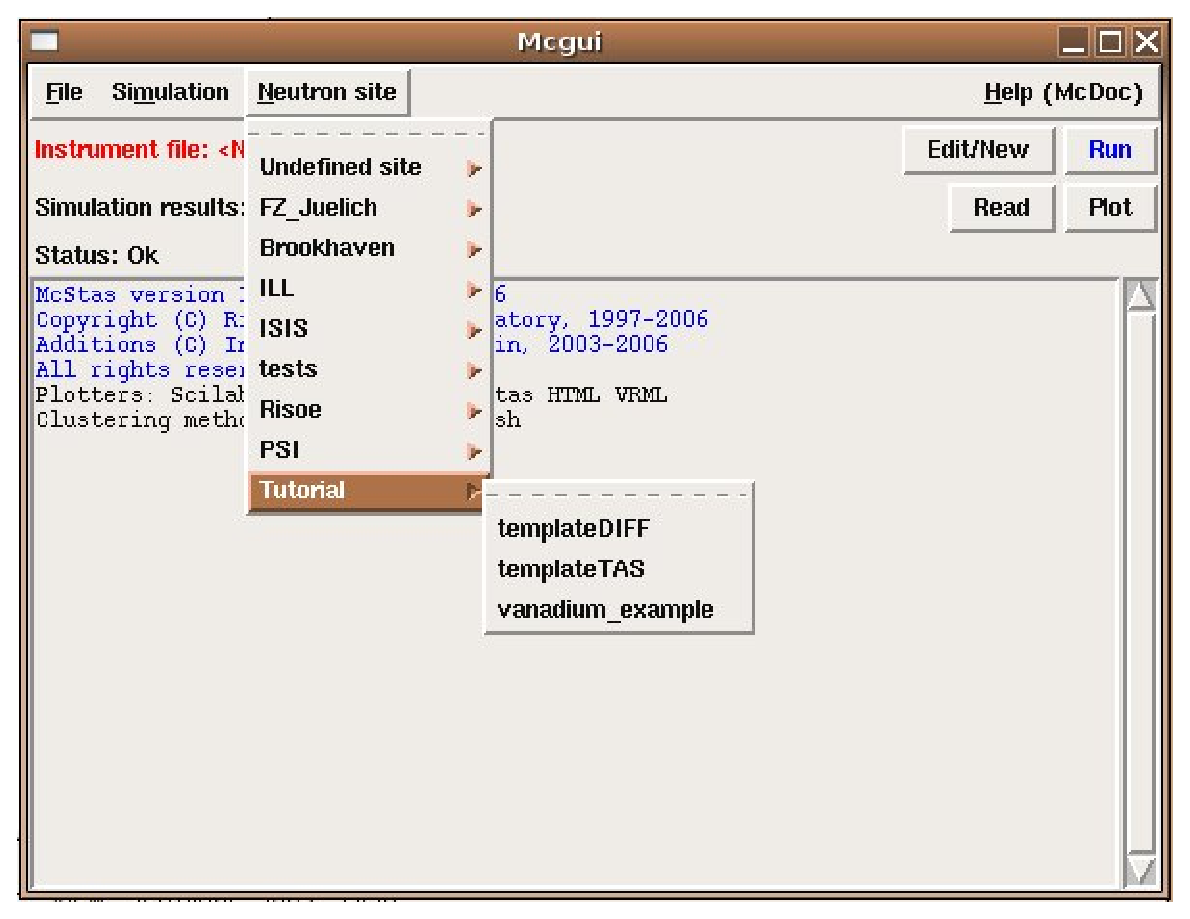
\includegraphics[width=0.55\textwidth]{figures/mcgui}
  \end{center}
\caption{The graphical user interface \texttt{mcgui}.}
\label{fig:mcgui}
\end{figure}
\label{p:neutronsite}
To load an instrument, select ``Tutorial'' from the ``Neutron site''
menu and open the file \verb+Samples_vanadium+. Next, check that the current plotting backend setting
(select ``Choose backend'' from the ``Simulation'' menu) corresponds
to your system setup.
\begin{itemize}
\item{by editing
the \verb+tools/perl/mcstas_config.perl+ setup file of your
installation}
\item{by setting the \verb+MCSTAS_FORMAT+ environment
variable.}
\end{itemize}
\indexEV{MCSTAS\_FORMAT}

Next, select ``Run simulation'' from the ``Simulation'' menu.
The \MCS compiler \mcs will translate the definition into an executable program.
Then \texttt{mcgui} will pop up a dialog window.
Type a value for the ``ROT'' parameter ({\em e.g.}
90), check the ``Plot results'' option, and select ``Start''. The
simulation will run, and when it finishes after a while the results will
be plotted in a window. Depending on your chosen plotting backend, the
presented graphics will resemble one of those shown in figure
\ref{fig:mcplot_figs}.\indexMCTOOL{mcplot}{}
\begin{figure}[htb!]
  \begin{center}
    \includegraphics[angle=-90,width=0.49\textwidth]{figures/mcplot_PGPLOT}
    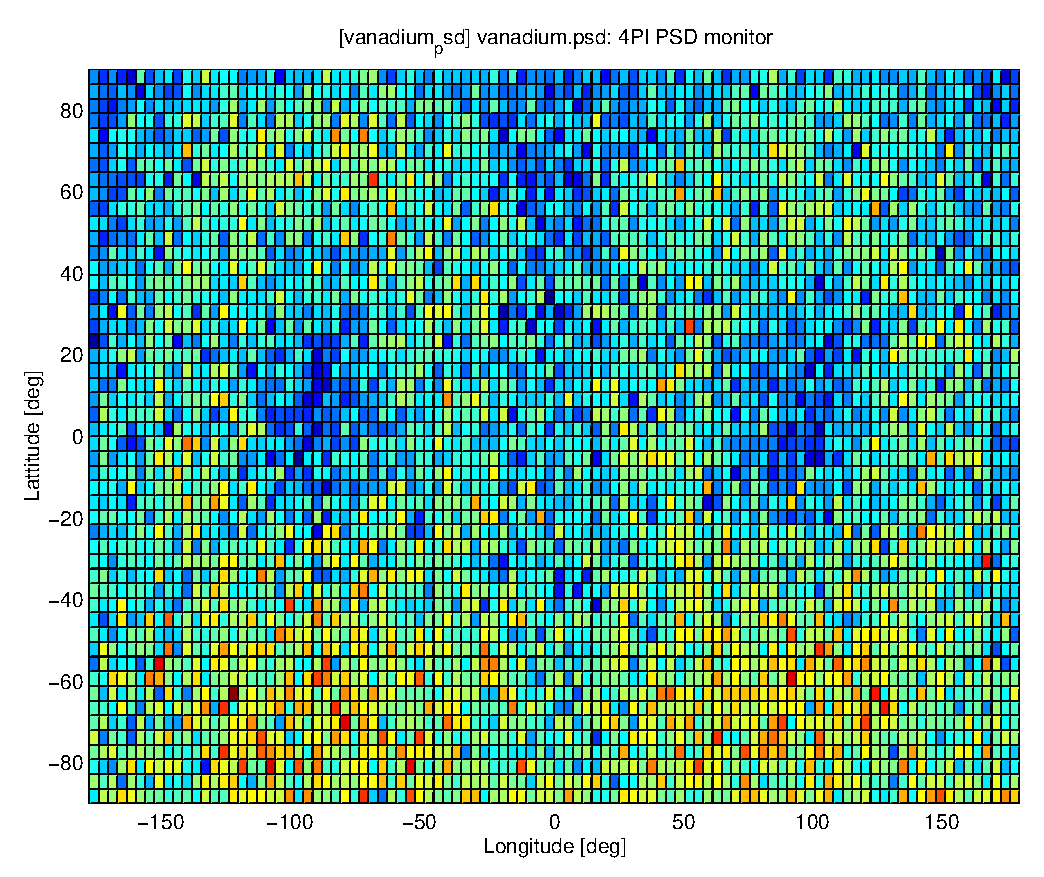
\includegraphics[width=0.49\textwidth]{figures/mcplot_Matlab}
  \end{center}
\caption{Output from \texttt{mcplot} with PGPLOT and Matlab backends}
\label{fig:mcplot_figs}
\end{figure}
When using the Matlab backend, full 3D view of plots and different
display possibilities are available. Use the attached \MCS window menus to
control these. Features are quite self explanatory. For other options, execute
\verb+mcplot --help+ (\verb+mcplot.pl --help+ on windows) to get help.

\indexTOOL{PGPLOT}
\indexTOOL{Matlab}
To visualize or
debug the simulation graphically, repeat the steps but check the ``Trace''
option instead of the ``Simulate'' option.  A window will pop up showing a
sketch of the instrument.  Depending on your chosen plotting backend, the
presented graphics will resemble one of those shown in figures
\ref{fig:mcdisp_PGPLOT}-\ref{fig:mcdisp_Matlab}.
\begin{figure}[htb!]
  \begin{center}
    \includegraphics[width=0.48\textwidth]{figures/mcdisplay_PGPLOT}
    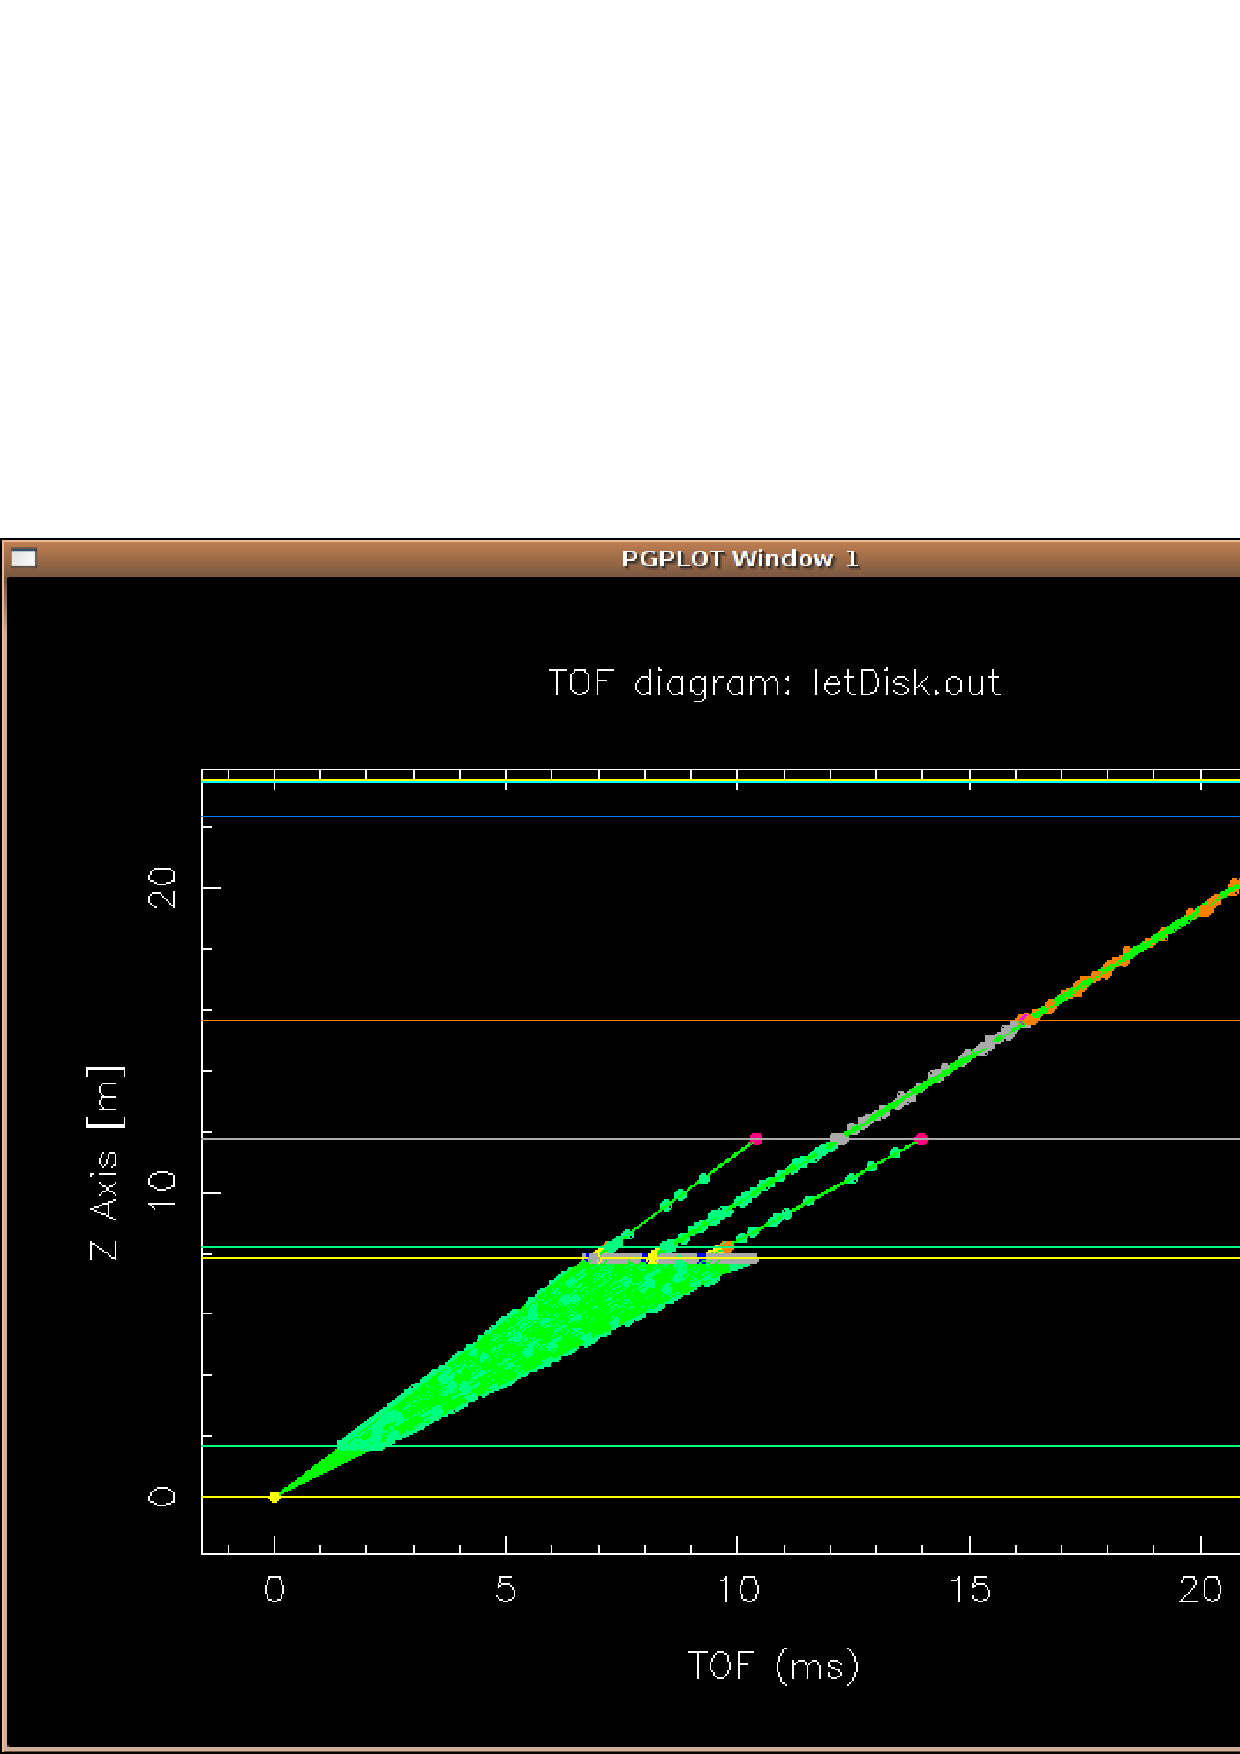
\includegraphics[width=0.48\textwidth]{figures/mcdisplay_TOF}
  \end{center}
  \caption{Left: Output from \texttt{mcdisplay} with PGPLOT backend.  The left
    mouse button starts a new neutron ray, the middle button zooms, and the
    right button resets the zoom. The Q key quits the program. Right: The new
    PGPLOT time-of-flight option. See section \ref{s:mcdisplay} for details.}
\label{fig:mcdisp_PGPLOT}
\end{figure}
\begin{figure}[htb!]
  \begin{center}
    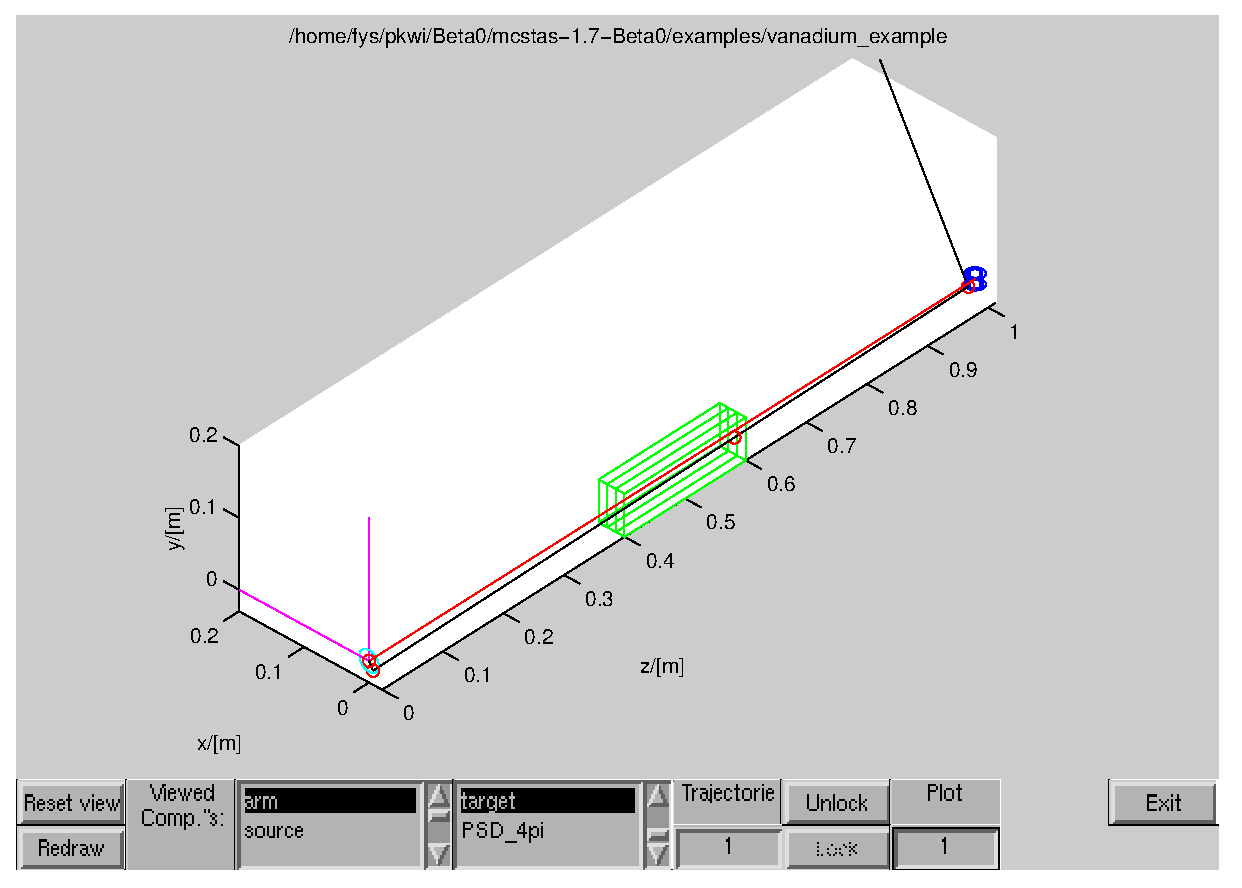
\includegraphics[width=0.55\textwidth]{figures/mcdisplay_Matlab}
  \end{center}
  \caption{Output from \texttt{mcdisplay} with Matlab backend. Display can be
    adjusted using the window buttons.}
\label{fig:mcdisp_Matlab}
\end{figure}

For a slightly longer gentle introduction to \MCS, see the \MCS tutorial
(available from~\cite{mcstas_webpage}), and as of version \version\ built into
the \verb+mcgui+ help menu. For more technical details, read on from
section~\ref{s:running}

\indexMCTOOL{mcgui}{)}
\index{McStas!running from the GUI|)}


%%%%%%%%%%%%%%%%%%%%%%%%%%%%%%%%%%%%%%%%%%%%%%%%%%%%%%%%%%%%%%%%%%%%%%%%%%%%%%%%
\section{Running the instrument compiler}
\label{s:running}

\indexMCSW{mcstas}{compiler}{(textbf}
This section describes how to run the \MCS compiler \mcs\ manually. Often,
it will be more convenient to use the front-end program \verb+mcgui+
(section~\ref{s:mcgui}) or \verb+mcrun+ (section~\ref{s:mcrun}),
which run the compilation and the simulations automatically.

Upon a command of the form
\begin{bash}
    mcstas name.instr
\end{bash}
the compiler \mcs will read the instrument definition \verb+name.instr+,
written in the \MCS meta-language,
and translate it into a Monte Carlo simulation program in
the programming language C.
The output is by default written to a file in the current
directory with the same name as the instrument file, but with extension
\verb+.c+ rather than \verb+.instr+. This can be overridden using the
\verb+-o+ option as follows:
\begin{bash}
    mcstas -o code.c name.instr
\end{bash}
which gives the output in the file \verb+code.c+.
A single dash `\verb+-+' may be used for both input and output filename
to represent standard input and standard output, respectively.


%-------------------------------------------------------------------------------
\subsection{Code generation options}
\index{Code generation!options}

By default, the code generated by \mcs is ISO-C with
some extensions (currently the only extension is the creation of new
directories, which is not possible in pure ISO-C). The use of
extensions may be disabled with the \verb+-p+ or \verb+--portable+
option. With this option, the output is strictly ISO-C compliant, at
the cost of some slight reduction in capabilities.

The \verb+-t+ or \verb+--trace+ option puts special ``trace'' code in
the output. This code makes it possible to get a complete trace of the
path of every neutron ray through the instrument, as well as the position
and orientation of every component. This option is mainly used with the
\verb+mcdisplay+ front-end as described in section~\ref{s:mcdisplay}.

The code generation options can also be controlled by using preprocessor
macros in the C compiler, without the need to re-run \mcs.
If the preprocessor macro \verb+MC_PORTABLE+ is defined, the
same result is obtained as with the \verb+--portable+ option.
The effect of the \verb+--trace+ option may be obtained
by defining the \verb+MC_TRACE_ENABLED+ macro. Most Unix-like C
compilers allow preprocessor macros to be defined using the \verb+-D+
option, e.g.
\begin{bash}
    cc -DMC_TRACE_ENABLED -DMC_PORTABLE ...
\end{bash}
Finally, the \verb+--verbose+ option will list the components and libraries being
included in the instrument.

%-------------------------------------------------------------------------------
\subsection{Specifying the location of files}
\label{s:files}

The \MCS compiler \mcs
needs to be able to find various files during compilation,
some explicitly requested by the user (such as component definitions and files
referenced by \verb+%include+), \indexKW{\%include}
and some used internally to generate the simulation executable.
\index{File!search path}
\index{Path!file search}
\MCS looks for
these files in three places: first in the current directory, then in a list of
directories given by the user, and finally in a special \MCS directory.
Usually, the user will not need to worry about this as \mcs will
automatically find the required files. But if users build their own component
library in a separate directory or if \mcs is installed in an unusual way, it
will be necessary to tell the compiler where to look for the files.

\index{Library!components}
\index{Installation!directory}
The location of the special \MCS directory is set
when \mcs is compiled.
It defaults to \nolinkurl{/usr/share/mcstas/version} on Debian and derivatives,
to \nolinkurl{/usr/local/mcstas/version} on RedHat and derivatives
and on other Unix-like systems, including Mac OS~X,
where it is a link to the actual location
\nolinkurl{/Applications/McStas-version.app/Contents/Resources/mcstas/version},
and \nolinkurl{C:\\mcstas-version\\lib} on Windows systems,
but it can be changed to something else,
see the installation instructions for details.

The location can be
overridden by setting the environment variable \verb+MCSTAS+:
\indexEV{MCSTAS}
\begin{bash}
    setenv MCSTAS /home/joe/mcstas
\end{bash}
for csh/tcsh users, or
\begin{bash}
    export MCSTAS=/home/joe/mcstas
\end{bash}
for bash/Bourne shell users.  Windows users should define
\verb+MCSTAS+ from the menu 'Start/Settings/Control
Panel/System/Advanced/Environment Variables' by creating \verb+MCSTAS+ with the
value \verb+C:\mcstas\lib+

To make \mcs search additional directories for component definitions
and include files, use the \verb+-I+ switch:
\begin{lstlisting}
    mcstas -I/home/joe/components -I/home/joe/neutron/include name.instr
\end{lstlisting}
Multiple \verb+-I+ options can be given, as shown.

%-------------------------------------------------------------------------------
\subsection{Embedding the generated simulations in other programs}

By default, \mcs will generate a stand-alone C program, which is what is needed
in most cases. However, for advanced usage, such as embedding the generated
simulation in another program or even including two or more simulations in the
same program, a stand-alone program is not appropriate.
For such usage, \mcs provides the following options:
\begin{itemize}
\item \verb+--no-main+ This option makes \mcs omit the \verb+main()+ function
  in the generated simulation program. The user must then arrange for the
  function \verb+mcstas_main()+ to be called in some way.
\item \verb+--no-runtime+ Normally, the
  generated simulation program contains all the run-time C code necessary for
  declaring functions, variables, etc. used during the simulation.  This
  option makes \mcs omit the run-time code from the generated
  simulation program, and the user must then explicitly link with the file
  \verb+mcstas-r.c+ as well as other shared libraries
  from the \MCS distribution.
  \index{Library!run-time}
\end{itemize}
Users that need these options are encouraged to contact the authors for further
help.

\indexMCSW{mcstas}{compiler}{)|)}

%-------------------------------------------------------------------------------
\subsection{Running the C compiler}
\label{s:compile}

After the source code for the simulation program has been generated with \mcs,
it must be compiled with the C compiler to produce an executable.
Since the generated C code obeys the ISO-C standard, it should be easy
to compile it using any ISO-C (or C++) compiler. \textit{E.g}.\ a typical
Unix-style command would be
\begin{lstlisting}
    cc -O -o name.out name.c -lm
\end{lstlisting}
The \MCS team recommends these compiler alternatives for the Intel (and AMD)
hardware architectures:
\begin{itemize}
\item[\textbf{A}]{\verb+gcc+ which is a very portable, open source, ISO-C compatible
    c compiler, available for most platforms. For Linux it is usually part of
    your distribution, for Windows the \MCS distribution package includes a
    version of \verb+gcc+ (in the Dev-CPP sub-package), and for Mac OS X
    \verb+gcc+ is part of the Xcode tools package available on the installation
    medium.}
\item[\textbf{B}]{\verb+icc+ or the Intel c compiler is available for Linux, Mac OS
    and Windows systems and is a commercial software product. Generally,
    simulations run with the Intel compiler are \textbf{a factor of 2 faster} than
    the identical simulation run using \verb+gcc+. To use \verb+icc+ with \MCS
    on Linux or Mac OS X, set the environment variables
    \begin{itemize}
      \item{\verb+MCSTAS_CC=icc+}
      \item{\verb+MCSTAS_CFLAGS="-g -O2 -wd177,266,1011,181"+}
    \end{itemize}
    To use \verb+icc+ with MPI on Unix system (see Section \ref{s:run-mpi})
 installations, it seems that \emph{editing}
    the mpicc shell script and setting the CC variable to "\verb+icc+" is the
    only requirement!}
  On Windows, the Intel c compiler is 'icl', not 'icc' and has a dependency for
  Microsoft Visual C++. If you have both these softwares available, running
  \MCS with the Intel compiler should be possible (currently untested by the
  \MCS developer team).

\end{itemize}


The \verb+-O+ option typically enables the optimization phase of the compiler,
which can make quite a difference in speed of \mcs-generated simulations. The
\verb+-o name.out+ sets the name of the generated executable. The \verb+-lm+
options is needed on many systems to link in the math runtime library (like the
$\cos()$ and $\sin()$ functions). \index{Optimization!compiler option}

Monte Carlo simulations are computationally intensive, and it is often desirable
to have them run as fast as possible. Some success can be obtained by adjusting
the compiler optimization options. Here are some example platform and compiler
combinations that have been found to perform well (up-to-date information will
be available on the \MCS WWW home page~\cite{mcstas_webpage}):
\begin{itemize}
\item Intel x86 (``PC'') with Linux and GCC, using options \verb+gcc -O3+.
\item Intel x86 with Linux and EGCS (GCC derivate) using
  options \verb+egcc -O6+.
\item Intel x86 with Linux and PGCC (pentium-optimized GCC derivate), using
  options \verb+gcc -O6 -mstack-align-double+.
\item HPPA machines running HPUX with the optional ISO-C compiler,
  using the options
  \verb|-Aa +Oall -Wl,-a,archive| (the \verb+-Aa+ option is necessary to
  enable the ISO-C standard).
\item SGI machines running Irix with the options
  \verb|-Ofast -o32 -w|
\end{itemize}
Optimization flags will typically result in a speed improvement by a factor
about 3, but the compilation of the instrument may be 5 times slower.

A warning is in place here: it is tempting to spend far more time fiddling with
compiler options and benchmarking than is actually saved in computation
times. Even worse, compiler optimizations are notoriously buggy; the options
given above for PGCC on Linux and the ISO-C compiler for HPUX have been known to
generate \emph{incorrect code} in some compiler versions. \mcs actually puts an
effort into making the task of the C compiler easier, by in-lining code and
using variables in an efficient way. As a result, \MCS simulations generally
run quite fast, often fast enough that further optimizations are not
worthwhile. Also, optimizations are highly time and memory consuming during
compilation, and thus may fail when dealing with large instrument descriptions
(e.g. more that 100 elements). The compilation process is simplified when using
components of the library making use of shared libraries (see \verb+SHARE+
keyword in chapter~\ref{c:kernel}). Refer to section \ref{s:optim} for other
optimization methods.\index{Optimization}

%%%%%%%%%%%%%%%%%%%%%%%%%%%%%%%%%%%%%%%%%%%%%%%%%%%%%%%%%%%%%%%%%%%%%%%%%%%%%%%%
\section{Running the simulations}
\label{s:run-sim}
\index{Parameters!instruments}

Once the simulation program has been generated by the \MCS compiler \mcs
and an executable has been obtained with the C compiler, the simulation
can be run in various ways.

\subsubsection{Simple \MCS options}
In this section, the most common simulation parameters are
discussed. For a full list, please consult tables
\ref{f:simoptions},~\ref{f:simoptions2}.

The simplest way is to run it directly from the
command line or shell:
\begin{lstlisting}
    ./name.out
\end{lstlisting}
Note the leading ``.'', which is needed if the current directory is not in the
path searched by the shell. When used in this way, the simulation will prompt
for the values of any instrument parameters such as angular settings, and then
run the simulation. Default instrument parameter values (see
section~\ref{s:instrdefs}), if any, will be indicated and entered when hitting
the \verb+Return+ key.\index{Parameters!optional, default value} This way of
running \MCS will only give data for one instrument setting which is normally
sufficient for {\em e.g.}, time-of-flight, SANS or powder instruments, but not
for {\em e.g.} continuous-beam reflectometers or triple-axis spectrometers where
a scan over various instrument settings is required.  Often the simulation will
be run using one of several available front-ends, as described in the next
section. These front-ends help manage output from the potentially many detectors
in the instruments, as well as running the simulation for each data point in a
scan.

The generated simulations accept a number of options and arguments. The
full list can be obtained using the \verb+--help+ option:
\begin{lstlisting}
    ./name.out --help
\end{lstlisting}
The values of instrument parameters may be specified as arguments using
the syntax \textit{name}\verb+=+\textit{val}. For example
\begin{lstlisting}
    ./Samples_vanadium.out ROT=90
\end{lstlisting}
\index{Parameters!instruments}
The number of neutron histories to simulate may be set using the
\verb+--ncount+ or \verb+-n+ option, for example
\verb+--ncount=2e5+. The initial seed for the random number generator is
by default chosen based on the current time so that it is different for
each run. However, for debugging purposes it is sometimes convenient to
use the same seed for several runs, so that the same sequence of random
numbers is used each time. To achieve this, the random seed may be set
using the \verb+--seed+ or \verb+-s+ option.

By default, \MCS simulations write their results into several data files in the
current directory, overwriting any previous files stored there. The
\verb+--dir=+\textit{dir} or \verb+-d+\textit{dir} option causes the files to be
placed instead in a newly created directory \textit{dir} (to prevent overwriting
previous results an error message is given if the directory already exists).
Alternatively, all output may be written to a single file \textit{file} using
the \verb+--file=+\textit{file} or \verb+-f+\textit{file} option (which should
probably be avoided when saving in binary format, see below). If the \verb+file+
is given as \verb+NULL+, the file name is automatically built from the
instrument name and a time stamp. The default file name is \verb+mcstas+
followed by appropriate extension.

The complete list of options
and arguments accepted by \MCS simulations appears in
Tables \ref{f:simoptions} and \ref{f:simoptions2}.

%-------------------------------------------------------------------------------
\subsection{Choosing an output data file format}

Data files contain header lines with information about the simulation from which
they originate. In case the data must be analyzed with programs that cannot read
files with such headers, they may be turned off using the \verb+--data-only+ or
\verb+-a+ option.  

\index{Data formats}
The format of the output files from \MCS simulations is described in more
detail in section~\ref{s:analyze}. It may be chosen either with
\verb+--format=FORMAT+ for each simulation or globally by setting the
MCSTAS\_FORMAT environment variable.
\indexEV{MCSTAS\_FORMAT}
The available format list is obtained using the \verb+name.out --help+ option.
\indexTOOL{PGPLOT}
\indexTOOL{Matlab}
\MCS can presently generate the \MCS /PGPLOT and the NeXus format. 

It is also possible to create and read \textit{Vitess}, \textit{MCNP/PTRAC} and
\textit{Tripoli4/batch} neutron event files using components
\begin{itemize}
\item \verb+Vitess_input+ and \verb+Vitess_output+
\item \verb+Virtual_tripoli4_input+ and \verb+Virtual_tripoli4_output+
\item \verb+Virtual_mcnp_input+ and \verb+Virtual_mcnp_output+
\end{itemize}\index{Vitess} \index{Tripoli} \index{MCNP}

Additionally, adding the \texttt{raw} keyword to the FORMAT will produce raw
$[N, p, p^2]$ data sets instead of $[N, p, \sigma]$ (see Section
\ref{s:staterror}). The former representation is fully additive, and thus
enables to add results from separate simulations (e.g. when using a computer
Grid - which is automated in the \verb+mcformat+ tool). Other acceptable format
modifiers are \verb+transpose+ to transpose data matrices and \verb+append+ to
concatenate data to existing files.

%-------------------------------------------------------------------------------
\subsection{Basic import and plot of results}
\label{s:run-format}
The previous example will result in a \verb+mcstas.sim+ file, that may be read
directly from Matlab (using the \textit{sim file} function)
\begin{matlab}
    matlab> s=mcstas;
    matlab> s=mcstas('plot')
\end{matlab}
\indexTOOL{Matlab}
The first line returns the simulation data as a single structure variable,
whereas the second one will additionally plot each detector separately.  This
also equivalently stands for IDL 
\begin{lstlisting}
    idl> s=mcstas()
    idl> s=mcstas(/plot)
\end{lstlisting}
\indexTOOL{IDL}
See section~\ref{s:mcplot} for another way of plotting simulation results
using the \verb+mcplot+ front-end.
\indexMCTOOL{mcplot}{}

When choosing the HTML format, the simulation results are saved as a web page,
whereas the monitor data files are saved as VRML files, displayed within the web
page.
\indexTOOL{VRML/OpenGL}\index{OpenGL}

\begin{table}
  \begin{center}
    {\let\my=\\
    \begin{tabular}{|p{0.24\textwidth}|p{0.7\textwidth}|}
      \hline
      \texttt{-s \textit{seed}} \my \texttt{--seed=\textit{seed}}
        & Set the initial seed for the random number generator. This may be
        useful for testing to make each run use the same random number
      sequence. \\
      \hline
      \texttt{-n \textit{count}} \my \texttt{--ncount=\textit{count}}
        & Set the number of neutron histories to simulate. The default
      is 1,000,000. (1e6)\\
      \hline
      \texttt{-d \textit{dir}} \my \texttt{--dir=\textit{dir}}
        & Create a new directory \textit{dir\/} and put all data files in
      that directory. \\
      \hline
      \texttt{-h} \my \texttt{--help}
        & Show a short help message with the options accepted, available formats
        and the names of the parameters of the instrument. \\
      \hline
      \texttt{-i} \my \texttt{--info}
        & Show extensive information on the simulation and the
      instrument definition it was generated from. \\
      \hline
      \texttt{-t} \my \texttt{--trace}
        & Makes the simulation output the state of every
      neutron as it passes through every component. Requires that the
      \texttt{-t} (or \texttt{--trace}) option is also given to the
      \MCS compiler \mcs when the simulation is generated. \\
      \hline
      \texttt{--no-output-files}
        & Disables the writing of data files (output to the
      terminal, such as detector intensities, will still be written). \\
      \hline
      \texttt{-g} \my \texttt{--gravitation}
        & Toggles the gravitation (approximation) handling
        for the whole neutron propagation within the instrument. May
        produce wrong results if the used components do no comply with
        this option.\\
      \hline
      \texttt{--format=\textit{FORMAT}}
        & Sets the file format for result simulation and data files. \\
      \hline
      \texttt{-N \textit{STEPS}}
        & Divide simulation into STEPS, varying parameters within given ranges 'min,max'. \\
      \hline
      \texttt{\textit{param}{\texttt =}\textit{value} \my \textit{min,max}}
        & Set the value of an instrument parameter, rather than having
        to prompt for each one. Scans ranges are specified as 'min,max'.\\
      \hline
    \end{tabular}
    \caption{Options accepted by \MCS simulations. For options
      specific to MPI and parallel computing, see section \ref{s:run-mpi}.}
    \label{f:simoptions}
    }
  \end{center}
\end{table}

\begin{table}
  \begin{center}
    {\let\my=\\
    \begin{tabular}{|p{0.35\textwidth}|p{0.6\textwidth}|}
      \hline
      \texttt{-f \textit{file}} \my \texttt{--file=\textit{file}}
        & Write all data into a single file \textit{file}. Avoid when using binary formats. \\
      \hline
      \texttt{--format\_data=\textit{FORMAT}}
        & Sets the file format for result data files from monitors. This enables to have simulation files in one format (e.g. HTML), and monitor files in an other format (e.g. VRML).\\
      \hline
      \texttt{--mpi=\textit{NB\_CPU}}
        & Distributes the simulation over NB\_CPU node (requires MPI
        to be installed). Speedup has been demonstrated to be linear
        in number of nodes when the simulation task is \verb+--ncount+
        is sufficiently large.\\
      \hline
      \texttt{--multi=\textit{NB\_CPU}} \my \texttt{--grid=\textit{NB\_CPU}}
        & Distributes the simulation over NB\_CPU node (requires SSH to be installed). Speedup has been demonstrated to be linear
        in number of nodes when the simulation task is \verb+--ncount+
        is sufficiently large.\\
      \hline
      \texttt{--machines=\textit{MACHINES}}
        & Specify a list of distant machines/nodes to be used for MPI and grid clustering. Default is to use local SMP cluster.\\
      \hline
      \texttt{--optim}
        & Run in optimization mode to find best parameters in order to maximize all monitor integral values. Parameters to be varied are given just like scans (min,max).\\
      \hline
      \texttt{--optim=\textit{COMP}}
        & Same as \verb+--optim+ but for specified monitors. This option may be used more than once.\\
      \hline
      \texttt{--optim-prec=\textit{ACCURACY}}
        & Sets accuracy criteria to end parameter optimization (default is 10$^{-3}$).\\
      \hline
      \texttt{--test}
        & Run \MCS self test.\\
      \hline
      \texttt{-c} \my \texttt{--force-compile}
        & Force to recompile the instrument.\\
      \hline
    \end{tabular}
    \caption{Additional options accepted by \MCS simulations.}
    \label{f:simoptions2}
    }
  \end{center}
\end{table}

%-------------------------------------------------------------------------------
\subsection{Interacting with a running simulation}
\index{Signal handler|textbf}

Once the simulation has started, it is possible, under Unix, Linux and Mac OS X systems, to interact with the on-going simulation. This feature is not available when using MPI parallelization.

\MCS attaches a signal handler to the simulation process. In order to send a signal to the process, the process-id \textit{pid} must be known. Users may look at their running processes with the Unix 'ps' command, or alternatively process managers like 'top' and 'gtop'.
If a \textit{file.out} simulation obtained from \MCS is running, the process status command should output a line resembling

\begin{bash}
<user> 13277 7140 99 23:52 pts/2   00:00:13   file.out
\end{bash}

where \verb+user+ is your Unix login. The \textit{pid} is there '13277'.

Once known, it is possible to send one of the signals listed in Table~\ref{t:signals} using the 'kill' unix command (or the functionalities of your process manager), e.g.
\indexSIG{USR2}{}
\index{kill|textbf}
\begin{bash}
    kill -USR2 13277
\end{bash}

This will result in a message showing status (here 33 \% achieved), as well as the position in the instrument of the current neutron.
\begin{lstlisting}
# McStas: [pid 13277] Signal 12 detected SIGUSR2 (Save simulation)
# Simulation: file (file.instr)
# Breakpoint: MyDetector (Trace) 33.37 % (  333654.0/ 1000000.0)
# Date      : Wed May  7 00:00:52 2003
# McStas: Saving data and resume simulation (continue)
\end{lstlisting}
followed by the list of detector outputs (integrated counts and files). Finally, sending a \verb+kill 13277+ (which is equivalent to \verb+kill -TERM 13277+) will end the simulation before the initial 'ncount' preset.

A typical usage example would be, for instance, to save data during a
simulation, plot or analyze it, and decide to interrupt the simulation earlier
if the desired statistics has been achieved. This may be done automatically
using the \verb+Progress_bar+ component.

Whenever simulation data is generated before end (or the simulation is
interrupted), the 'ratio' field of the monitored data will provide the level of
achievement of the computation (for instance '3.33e+05/1e+06'). Intensities are
then usually to be scaled accordingly by the user.

Additionally, any system error will result in similar messages, giving
indication about the occurrence of the error (component and section). Whenever
possible, the simulation will {\em try} to save the data before ending. Most
errors appear when using a newly written component, in the \texttt{INITIALIZE},
\texttt{TRACE} or \texttt{FINALLY} sections. Memory errors usually show up when
C pointers have not been allocated/unallocated before usage, whereas
mathematical errors are found when, for instance, dividing by zero.
\index{Bugs!system errors}

\begin{table}
  \begin{center}
    {\let\my=\\
    \begin{tabular}{|p{0.24\textwidth}|p{0.7\textwidth}|}
      \hline
      \texttt{USR1} & Request information (status)  \\
      \texttt{USR2, HUP} & Request information and performs an intermediate
      saving of all monitors (status and save). This triggers the execution of
      all \texttt{SAVE} sections (see chapter~\ref{c:kernel}).  \\
      \texttt{INT, TERM} & Save and exit before end (status)  \\
      \hline
    \end{tabular}
    \caption{Signals supported by \MCS simulations.}
    \label{t:signals}
\indexSIG{USR1}{}
\indexSIG{USR2}{}
\indexSIG{HUP}{}
\indexSIG{INT}{}
\indexSIG{TERM}{}
    }
  \end{center}
\end{table}

%-------------------------------------------------------------------------------
\subsection{Optimizing simulation speed}
\label{s:optim}
\index{Optimization|textbf}

There are various ways to speed up simulations
\begin{itemize}
\item Optimize the compilation of the instrument, as explained in
  section~\ref{s:compile}.
\item Execute the simulation in parallel on a computer grid or a cluster (with
  MPI or ssh grid ) as explained in section~\ref{s:run-mpi}.
\item Divide simulation into parts using a file for saving or generating neutron
  events. In this way, a guide may be simulated only once, saving the neutron
  events at the guide exit as a file, which is being read quickly by the second
  simulation part. Use the Virtual\_input and Virtual\_output components for
  this technique.
\item Use source optimizers like the components Source\_adapt or
  Source\_Optimizer. Such component may sometimes not be very efficient, when no
  neutron importance sampling can be achieved, or may even sometimes alter the
  simulation results. Be careful and always check results with a (shorter)
  non-optimized computation.
\item Complex components usually take into account additional small effects in a
  simulation, but are much longer to execute. Thus, simple components should be
  preferred whenever possible, at least in the beginning of a simulation project.
\item The SPLIT keyword may artificially repeat events reaching specified
  positions in the instrument. This is \emph{very} efficient, but requires to
  cast random numbers in the course of the remaining propagation (e.g. at
  samples, crystals, ...). See section \ref{s:instrdefs-extend-enhance} for
  details.
\end{itemize}
A general comment about optimization is that it should be used cautiously,
checking that the results are not significantly affected.

%-------------------------------------------------------------------------------
\subsection{Optimizing instrument parameters}
\label{s:optimize}\index{Parameters!optimization}
Often, the user may wish to optimize the parameters of a simulation, i.e. the
best geometry of a given component, for example the optimal curvature of a
monochromator.

The choice of the optimization routine, of the simulation quality value to
optimize, the initial parameter guess and the simulation length all have a large
influence on the results.  The user is advised to be cautious when interpreting
the optimization results.

\subsubsection{Using iFit for optimization}

One of the authors of \MCS has developed a very flexible and general data
analysis and fitting package called iFit \cite{iFit,iFit_web} based on
Matlab. Matlab itself is not required, as a stand-alone distributable binary of
iFit exists.

iFit contains wrapper functionality for compiling and running \MCS simulations
as object functions, and allows to select many different optimizers, including
swarms and other non-gradient methods. Please see the iFit documentation for
more information.

Our experience is that iFit together with \MCS is a more robust optimization
solution than the \MCS built-in Simplex solution.

\subsubsection{Using the Simplex method}

The \MCS package comes with a Simplex optimization method to find best
instrument parameters in order to maximize all or some specified monitor
integrated values. It uses the Downhill Simplex Method in
Multidimensions~\cite{neldermead,NumRecip} which is a geometric optimization
method somewhat similar to genetic algorithms. It is not as fast as the gradient
method, but is much more robust. It is well suited for problems with up to about
10-20 parameters to optimize. Higher dimensionalities are not guarantied to
converge to a meaningful solution.

When using \verb+mcrun+ (section \ref{s:mcrun}), the optimization mode is set by
using the \verb+--optim+ option or a list of monitors to maximize with as many
\verb+--optim=COMP+ as required. The optimization accuracy criterion may be
changed with the \verb+--optim-prec=accuracy+ option.

From \verb+mcgui+ (section \ref{s:mcgui}), one should choose the 'Optimization'
execution mode (instead of the Simulation or Trace mode). Then specify the
instrument parameters to optimize by indicating their variation range
\verb+param=min,max+ (e.g. Lambda=1,4) just like parameter scans. Optionally,
the starting guess value might be given with the syntax
\verb+param=min,guess,max+. The optimization accuracy criterion is controlled
using the 'Precision' entry box in the configuration options (See Figure
\ref{fig:mcgui-choose}). Finally, run the simulation. The optimum set of
parameters is then printed at the end of the simulation process. You may ask to
maximize only given monitors (instead of all) by selecting their component names
in the lower lists in the Run Dialog (up to 3).

If you would like to maximize the flux at a given monitor, with some
divergence constrains, you should for instance simply add a divergence
collimator before the monitor. Alternatively, write a new component
that produce the required 'figure-of-merit'.

The optimization search interval constrains the evolution of
parameters. It should be chosen carefully. In particular it is safer
for it to indeed contain a high signal domain, and be preferably
symmetric with respect to that maximum.

\subsubsection{Using custom optimization routines}
The user should write a function script or a program that
\begin{itemize}
\item inputs the simulation parameters, which are usually numerical values such
  as $TT$ in the \verb+prisma2+ instrument from the \verb+examples+ directory of
  the package.
\item builds a command line from these parameters.
\item executes that command, and waits until the end of the computation.
\item reads the relevant data from the monitors.
\item outputs a simulation quality measurement from this data, usually the
  integrated counts or some peak width.
\end{itemize}

For instance, for the \verb+prisma2+ instrument we could write a function for
Matlab (see section~\ref{s:analyze} for details about the Matlab data format) in
order to study the effects of the $TT$ parameter:
\begin{lstlisting}
  function y = instr_value(p)
    TT = p(1);     % p may be a vector/matrix containing many parameters
    syscmd = [ 'mcrun prisma2.instr -n1e5 TT=' num2str(TT) ...
               ' PHA=22 PHA1=-3 PHA2=-2 PHA3=-1 PHA4=0 PHA5=1' ...
               ' PHA6=2 PHA7=3 TTA=44 --format="Matlab binary"' ];
    system(syscmd); path(path) % execute simulation, and rehash files
    s = mcstas;     % get the simulation data, and the monitor data
    s = s.prisma2.m_mcstas.detector.prisma2_tof.signal;
    eval(s);        % we could also use the 'statistics' field
    y = -Mean;      % 'value' of the simulation
\end{lstlisting}

Then a numerical optimization should be available, such as those provided with Matlab, IDL, and Perl-PDL high level languages. In this example, we may wish to maximize the \verb+instr_value+ function value. The \verb+fminsearch+ function of Matlab is a minimization method (that's why we have a minus sign for $y$ value), and:
\begin{lstlisting}
    matlab> TT = fminsearch('instr_value', -25)
\end{lstlisting}
will determine the best value of TT, starting from -25 estimate, in order to
minimize function \verb+instr_value+, and thus maximize the mean detector
counts.

%%%%%%%%%%%%%%%%%%%%%%%%%%%%%%%%%%%%%%%%%%%%%%%%%%%%%%%%%%%%%%%%%%%%%%%%%%%%%%%%
\section{Using simulation front-ends}
\label{s:frontends}

\MCS includes a number of front-end programs that extend the
functionality of the simulations. A front-end program is an interface
between the user and the simulations, running the simulations and
presenting the output in various ways to the user.

The list of available \MCS front-end programs may be obtained from the
\verb+mcdoc --tools+ command:
\begin{lstlisting}
    McStas Tools
       mcstas        Main instrument compiler
       mcrun         Instrument build and execution utility
       mcgui         Graphical User Interface instrument builder
       mcdoc         Component library documentation generator/viewer
       mcplot        Simulation result viewer
       mcdisplay     Instrument geometry viewer
       mcresplot     Instrument resolution function viewer
       mcstas2vitess McStas to Vitess component translation utility
       mcformat      Conversion tool for text files and MPI/grids
       mcformatgui   GUI for mcformat
       mcdaemon      Instrument results on-line plotting
    When used with the -h flag, all tools display a specific help.
    SEE ALSO: mcstas, mcdoc, mcplot, mcrun, mcgui, mcresplot, mcstas2vitess
    DOC:      Please visit http://www.mcstas.org
\end{lstlisting}

%-------------------------------------------------------------------------------
\subsection{The graphical user interface (mcgui)}
\label{s:mcgui}
\indexMCTOOL{mcgui}{textbf}

The front-end \verb+mcgui+ provides a graphical user interface that interfaces
the various parts of the \MCS package. It may be started with the single
command
\begin{lstlisting}
    mcgui
\end{lstlisting}
The mcgui (mcgui.pl on Windows) program may optionally be given the name of the
instrument file to use.

\paragraph{Dependencies:}
\indexTOOL{PGPLOT} To run the \verb+mcgui+
front-end, the programs Perl and Perl/Tk must be properly installed on the
system. Additionally, to use the \MCS/PGPLOT back-end the software packages
PGPLOT, PgPerl, and PDL are required.
\index{Perl!libraries} It may be
necessary to set the \verb+PGPLOT_DIR+ and \verb+PGPLOT_DEV+ environment
variable; consult the documentation for PGPLOT on the local system in case of
difficulty.
\indexEV{PGPLOT\_DIR}
\indexEV{PGPLOT\_DEV}

\subsubsection{The menus}

When the front-end is started the main window is opened (see figure
\ref{fig:mcgui}). This window displays the output from compiling and running
simulations, and contains a few menus and buttons for easy navigation. The main
purpose of the front-end is to edit and compile instrument definitions, run the
simulations, and visualize the results.

The \textbf{File} menu has the following features:
\begin{description}
\item[File/Open instrument] selects the name of an instrument file to be used.
\item[File/Edit current] opens a simple editor window with \MCS syntax
  highlighting for editing the
  current instrument definition. This function is also available from
  the \textbf{Edit} button to the right of the name of the instrument definition in
  the main window.
\item[File/Spawn editor] This starts the editor defined in the environment
  variable \verb+VISUAL+ or \verb+EDITOR+ on the current instrument
  file. It is also possible to start an external editor manually; in any
  case \verb+mcgui+ will recompile instrument definitions as necessary based on
  the modification dates of the files on the disk.
  \indexEV{EDITOR}
\item[File/Compile instrument] forces a recompile of the instrument definition,
  regardless of file dates. This is for example useful to pick up changes in
  component definitions, which the front-end will not notice automatically. This
  might also be required when choosing MPI \index{MPI|textbf} and NeXus options.
  \indexTOOL{NeXus}
\item[File/Save log file] saves the text in the window showing output of
  compilations and simulations into a file.
\item[File/Clear output] erases all text in the window showing output of
  compilations and simulations.
  \item[File/Preferences] Opens the choose backend dialog shown in
  figure~\ref{fig:mcgui-choose}. Several settings can be chosen here:
\begin{itemize}
  \item Selection of  the desired (PGPLOT|Matlab|HTML/VRML) output
    format and possibility to save 'binary files' when
  applicable (improved disk I/O).
  \item One- or three-pane view of your instrument in trace mode when
    using PGPLOT.
  \item Clustering option (None|MPI|ssh)
  \item Choice of editor to use when editing instrument files.
  \item Automatic quotation of strings when inserting in the built-in
    editor.
  \item Possibility to \emph{not} optimize when compiling the generated
    c-code. This is very handy when setting up an instrument model, which
    requires regular compilations.
  \item Adjustment of final precision when doing parameter optimization.
\end{itemize}
To save the chosen settings for your next \MCS run, use Save
Configuration in the File menu.
\item[File/Save configuration] saves user settings from Configuration
  options and Run dialogue to disk.
\item[File/Quit] exits the graphical user interface front-end.
\end{description}

\noindent The \textbf{Simulation} menu has the following features:
\begin{description}\indexMCTOOL{mcplot}{}\index{Data formats}
\item[Simulation/Read old simulation] prompts for the name of a file
  from a previous run of a \MCS simulation (usually called
  \verb+mcstas.sim+). The file will be read and any detector data
  plotted using the \verb+mcplot+ front-end. The parameters used in the
  simulation will also be made the defaults for the next simulation
  run. This function is also available using the ``Read'' button to the
  right of the name of the current simulation data.
\item[Simulation/Run simulation] opens the run dialog window, explained
  further below.
\item[Simulation/Plot results] plots (using \verb+mcplot+) the results of the
  last simulation run or spawns a load dialogue to load a set of results.
\end{description}


\begin{figure}[htb!]
  \begin{center}
    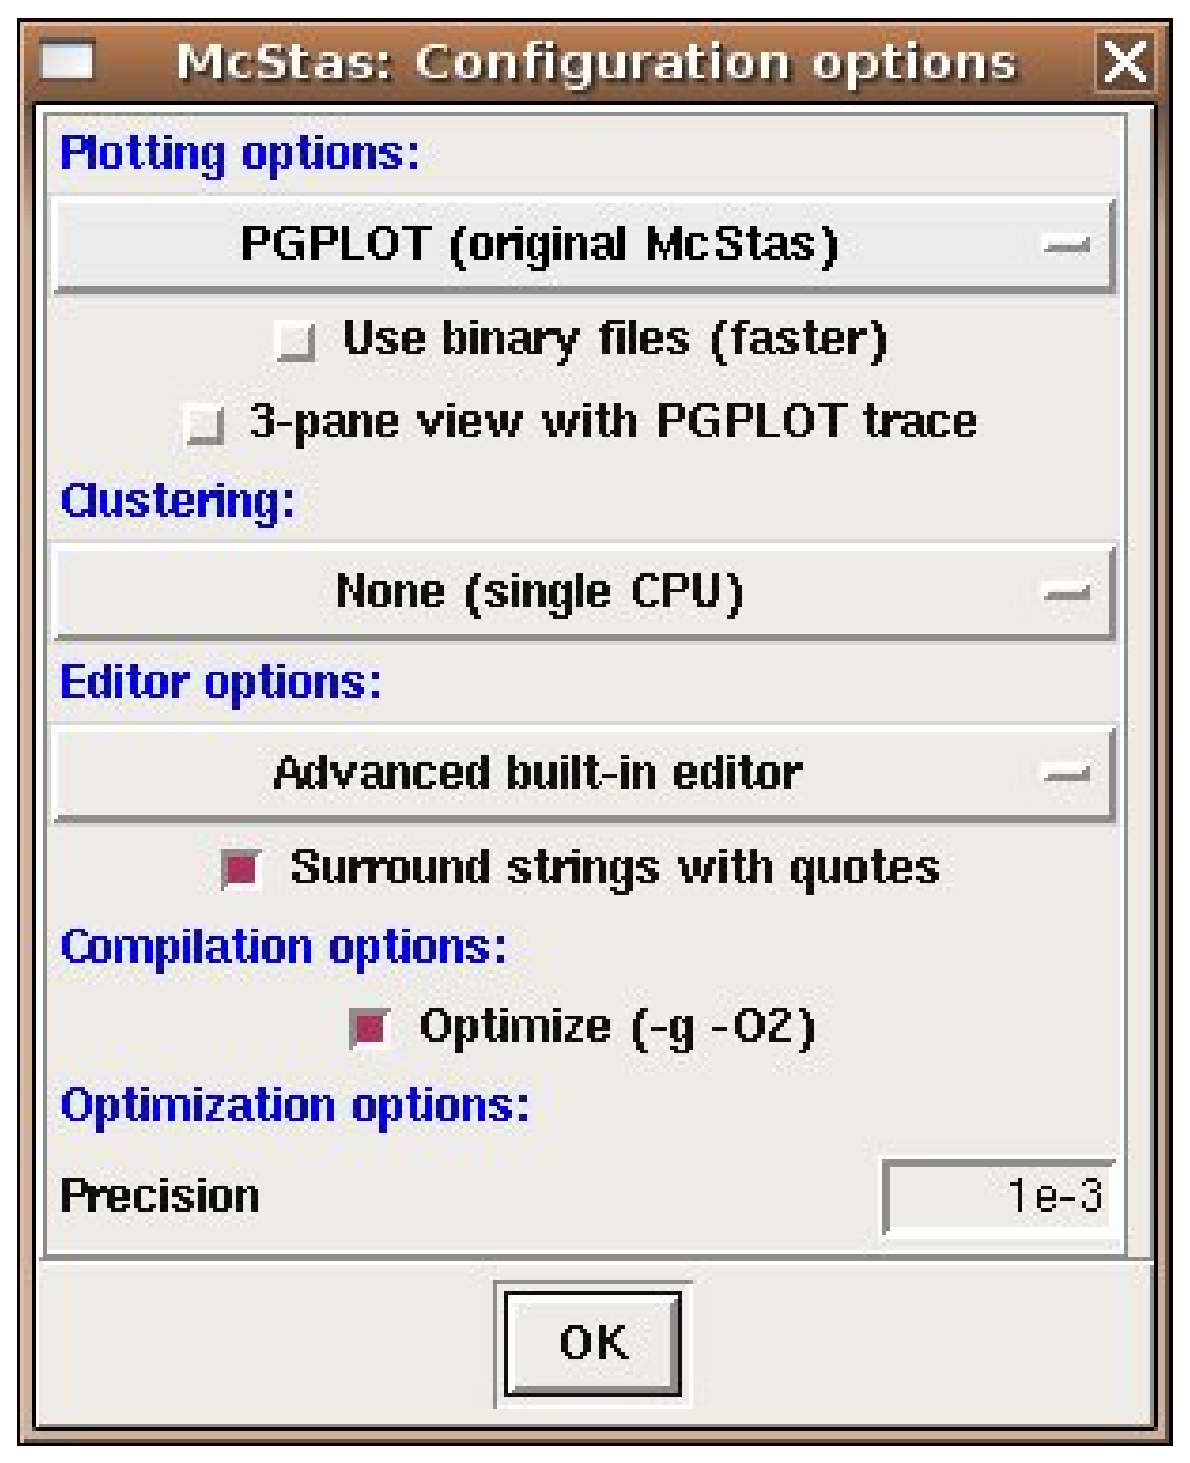
\includegraphics[width=0.3\textwidth]{figures/choose_backend}
  \end{center}
\caption{The ``configuration options'' dialog in \texttt{mcgui}.}
\label{fig:mcgui-choose}
\end{figure}


\noindent The \textbf{Neutron Site} menu contains a list of template/example
instruments as found in the \MCS library, sorted by neutron site. When
selecting one of these, a local copy of the instrument description is
transferred to the active directory (so that users have modification rights) and
loaded. One may then view its source (Edit) and use it directly for
simulations/trace (3D View).
\\\ \\

\noindent The \textbf{Tools} menu gathers minor tools.
\begin{description}
\item[Tools/Plot current/other results] Plot current simulation results and
  other results.
\item[Tools/Online plotting of results] installs a DSA key to be used for ssh
  clustering and MPI (see Section \ref{s:run-mpi}).
\item[Tools/Dataset convert/merge] Opens a GUI to the \verb+mcformat+ tool, in
  order to convert datasets to other formats, merge scattered dataset (e.g. from
  successive or grid simulations), and assemble scan sets. This tool does not
  handle raw event files.
\item[Tools/Shortcut keys] displays the shortcut keys used for running and
  editing instruments.
\item[Tools/Install DSA key] installs a DSA key to be used for ssh clustering
  and MPI (see Section \ref{s:run-mpi}).\index{MPI}\index{Grid computing}
\item[The Histogrammer] In addition to these tools, the
  \verb+Neutron site/Tools/Histogrammer.instr+ example instrument may read
  \MCS, Vitess, MCNP and Tripoli event files in order to generate histograms
  of any type.
\end{description}


\noindent The \textbf{Help} menu has the following features, through use of
\verb+mcdoc+ and a web browser. To customize the used web browser, set
the \verb+BROWSER+ environment variable. If \verb+BROWSER+ is not set,
\verb+mcgui+ uses \verb+netscape/mozilla/firefox+ on Unix/Linux and the default browser on
Windows.
\begin{description}
\item[Help/\MCS User manual] calls \verb+mcdoc --manual+, brings up the local
  pdf version of this manual, using a web browser.
\item[Help/\MCS Component manual] calls \verb+mcdoc --comp+, brings up the local
  pdf version of the component manual, using a web browser.
\item[Help/Component library index] displays the component documentation using
  the component \verb+index.html+ index file.
\item[Help/\MCS web page] calls \verb+mcdoc --web+, brings up the \MCS
  website in a web browser.
\item[Help/Tutorial] opens the \MCS tutorial for a quick start.
\item[Help/Current instrument info] generates a description web-page of the
  current edited instrument.
\item[Help/Test \MCS installation] launches a self test procedure to check that
  the \MCS package is installed properly, generates accurate results, and may
  use the plotter to display the results.
\item[Help/Generate component index] (re-)generates locally the component
  \verb+index.html+.
\end{description}


\subsubsection{The run dialog}

\begin{figure}[htb!]
  \begin{center}
    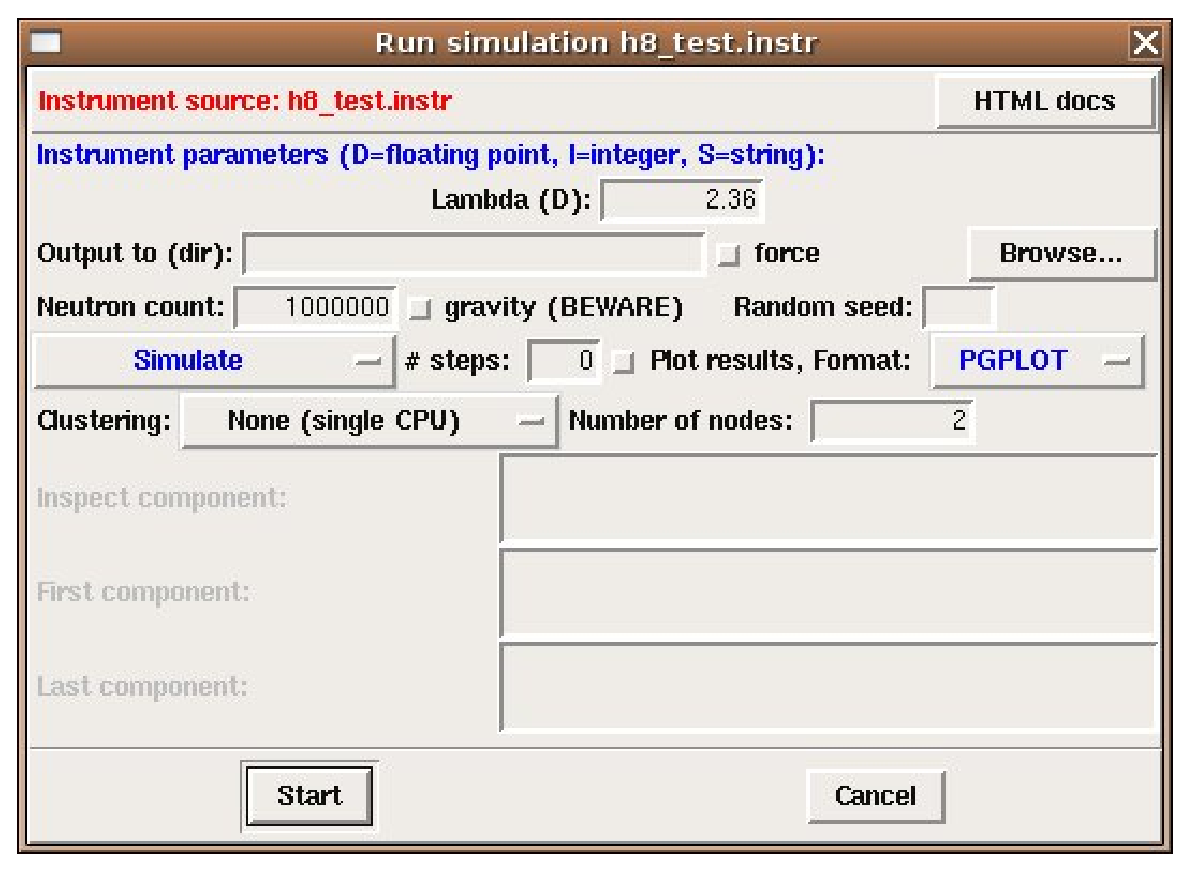
\includegraphics[width=0.45\textwidth]{figures/mcgui-run}
  \end{center}
\caption{The run dialog in \texttt{mcgui}.}
\label{fig:mcgui-run}
\end{figure}
%
The run dialog is used to run simulations. It allows the entry of instrument
parameters as well as the specifications of options for running the simulation
(see section~\ref{s:run-sim} for details). It also allows to run the
\verb+mcdisplay+ (section~\ref{s:mcdisplay}) and \verb+mcplot+
(section~\ref{s:mcplot}) front-ends together with the
simulation.\indexMCTOOL{mcplot}{}

The meaning of the different fields is as follows:
\begin{description}
\item[Run:Instrument parameters] allows the setting of the values for the input
  parameters of the instrument. The type of each instrument parameter is given
  in parenthesis after each name. Floating point numbers are denoted by (D) (for
  the C type ``\verb+double+''), (I) denotes integer parameters, and (S) denotes
  strings. For parameter scans and optimizations, enter the minimum and maximum
  values to scan/optimize, separated by a comma, e.g. \verb+1,10+ and do not
  forget to set the \textbf{\# Scanpoints} to more than 1.
\item[Run:Output to] allows the entry of a directory for storage of the
  resulting data files in (like the \verb+--dir+ option). If no name is given,
  the results are stored in the current directory, to be overwritten by the next
  simulation.
\item[Run:Force] Forces \MCS to overwrite existing data files
\item[Neutron count] sets the number of neutron rays to
  simulate (the \verb+--ncount+ option).
\item[Run:Gravity] Activates gravitation handling. Not all components full
  support the use of gravitation, but all transport in ``free space'' using the
  PROP\_DT, PROP\_Z0 etc. macros will include propagation with gravity. Only
  local, internal component propagation without the PROP routines will be
  gravity-less. As a conclusion it is considered safe and to high precision
  correct to apply the gravitation setting if one takes care to use the
  Guide\_gravity component and other gravity-supporting guide types in
  combination with non-gravity components that are ``small'' in size,
  i.e. samples, lenses, etc.
\item[Run:Random seed/Set seed to] selects between using a random seed (different
  in each simulation) for the random number generator, or using a fixed
  seed (to reproduce results for debugging).
\item[Run:Simulate/Trace (3D)/Optimize] selects between several modes of
  running the simulation:
  \begin{itemize}
  \item Simulate: perform a normal simulation or a scan when \#steps
    is set to non-zero value
  \item Trace (3D view): View the instrument in 3D tracing individual
    neutrons through the instrument
  \item Optimize: find the optimum value of the simulation parameters
    in the given ranges (see section \ref{s:optimize}).
  \item Backgrounding (bg): Simulate or Optimize in the background.
\end{itemize}
\item[Run:\# steps / \# optim] sets the number of simulation to run when
  performing a parameter scan or the number of iterations to
  perform in optimization mode.
\item[Run:Plot results] -- if checked, the \verb+mcplot+ front-end will be run
  after the simulation has finished, and the plot dialog will appear
  (see below).
\item[Run:Format] quick selection of output format. Binary mode may be checked
  from the ``Simulation/Configuration options'' dialog box.
\item[Run:Clustering method] selects the mechanism to be used for running on
  grids and clusters.  See section~\ref{s:run-mpi} on parallel computing for
  more informations.
\item[Run:Number of nodes] sets the number of nodes to use for MPI/ssh
  clustering.
\item[Run:Inspect component] (Trace mode) will trace only neutron trajectories
  that reach a given component (e.g. sample or detector).
\item[Run:First component] (Trace mode) seletcs the first component to plot
  (default is first) in order to define a region of interest.
\item[Run:Last component] (Trace mode) seletcs the last component to plot
  (default is first) in order to define a region of interest.
\item[Run:Maximize monitor] (Optimization mode) seletcs up to three monitors
  which integral value should be maximized, varying instrument parameters. If no
  monitor is selected, the sum of all monitors is optimized.
\item[Run:Start] runs the simulation.
\item[Run:Cancel] aborts the dialog.
\end{description}
Most of the settings on the run dialog can be saved for your next
\MCS run using 'Save configuration' in the File menu.

Before running the simulation, the instrument definition is automatically
compiled if it is newer than the generated C file (or if the C file is newer
than the executable). The executable is assumed to have a \verb+.out+ suffix in
the filename. NB: If components are changed, automatic compilation is \emph{not}
performed. Instead, use the File/Compile menu item in mcgui.



\subsubsection{The editor window}

The editor window provides a simple editor for creating and modifying instrument
definitions. Apart from the usual editor functions, the ``Insert'' menu provides
some functions that aid in the construction of the instrument definitions:
\begin{description}
\item[Editor Insert/Instrument template] inserts the text for a simple instrument
  skeleton in the editor window.
\item[Editor Insert/Component\ldots] opens up a dialog window with a list of all
  the components available for use in \MCS. Selecting a component will
  display a description. Double-clicking will open up a dialog window
  allowing the entry of the values of all the parameters for the
  component (figure~\ref{f:comp_dialog}). See section~\ref{s:instrdefs}
  for details of the meaning of the different fields.

  The dialog will also pick up those of the users own components that are
  present in the current directory when \verb+mcgui+ is started. See
  section~\ref{s:mcdoc} for how to write components to integrate well with this
  facility.
\item[Editor Insert/\textit{Type}] These menu entries give quick access to the
  entry dialog for the various component types available, i.e. Sources, Optics,
  Samples, Monitors, Misc, Contrib and Obsolete.
\end{description}
\begin{figure}[tbp]
  \begin{center}
    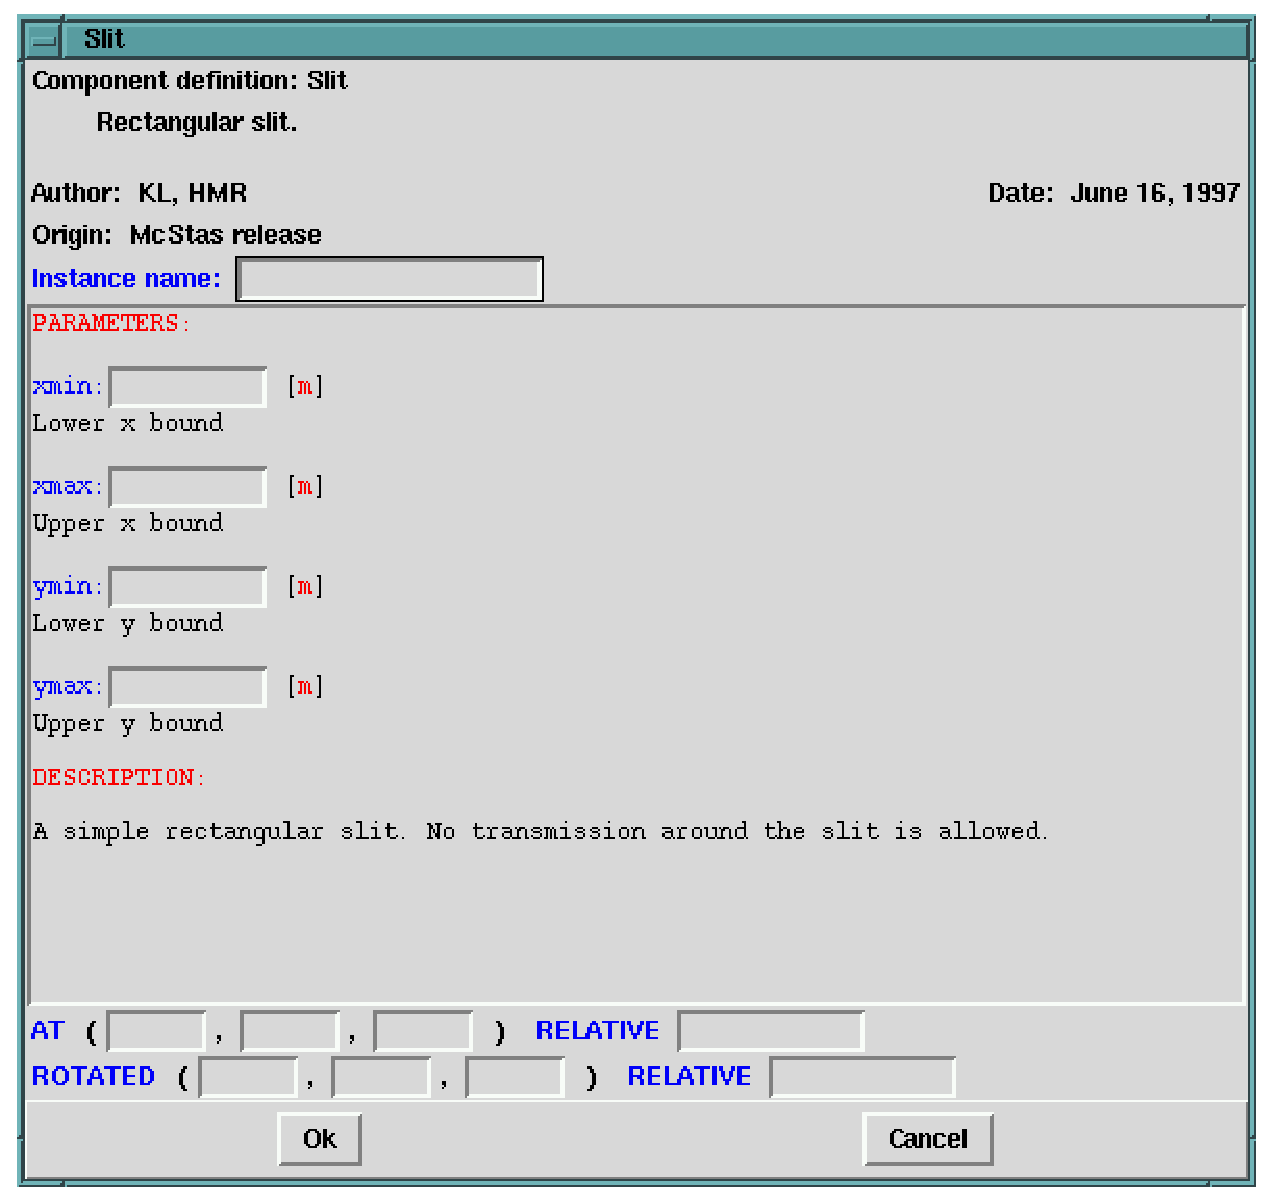
\includegraphics[width=0.55\textwidth]{figures/comp_dialog}
    \caption{Component parameter entry dialog.}
    \label{f:comp_dialog}
  \end{center}
\end{figure}


%-------------------------------------------------------------------------------
\subsection{Running simulations on the commandline (mcrun)}
\label{s:mcrun}
\indexMCTOOL{mcrun}{textbf}
\index{Parameters!instruments}
\index{Parameters!scans}
\index{Parameters!optimization}

The \verb+mcrun+ front-end (mcrun.pl on Windows) provides a convenient
command-line interface for running simulations with the same automatic
compilation features available in the \verb+mcgui+ front-end. It also provides a
facility for running a series of simulations while varying an input parameter.

The command

\begin{bash}
mcrun sim args ...
\end{bash}

will compile the instrument definition \texttt{\textit{sim}.instr} (if
necessary) into an executable simulation \texttt{\textit{sim}.out}. It
will then run \texttt{\textit{sim}.out}, passing the argument list \textit{
  args}

The possible arguments are the same as those accepted by the simulations
themselves as described in section~\ref{s:run-sim}, with the following
extensions:
\begin{itemize}
\item The \verb+-c+ or \verb+--force-compile+ option may be used to force the
  recompilation of the instrument definition, regardless of file dates. This may
  be needed in case any component definitions are changed (in which case
  \verb+mcrun+ does not automatically recompile), or if a new version of \MCS
  has been installed.
\item The \texttt{-p \textit{file}} or \texttt{--param=\textit{file}} option may be
  used to specify a file containing assignment of values to the input parameters
  of the instrument definition. The file should consist of specifications of the
  form \texttt{\textit{name\/}=\textit{value\/}} separated by spaces or line
  breaks. Multiple \verb+-p+ options may be given together with direct parameter
  specifications on the command line. If a parameter is assigned multiple times,
  later assignments override previous ones.
\item The \texttt{-N \textit{count}} or \texttt{--numpoints=\textit{count}} option
  may be used to perform a series of \textit{count\/} simulations while
  varying one or more parameters within specified intervals. Such a
  series of simulations is called a \emph{scan}. To specify
  an interval for a parameter \textit{X}, it should be assigned two
  values separated by a comma. For example, the command
\begin{bash}
mcrun sim.instr -N4 X=2,8 Y=1
\end{bash}
would run the simulation defined in \verb+sim.instr+ four times, with
\textit{X} having the values 2, 4, 6, and 8, respectively.

After running the simulation, the results will be written to the file
\verb+mcstas.dat+ by default. This file contains one line for each simulation
run giving the values of the scanned input variables along with the integrated
intensity and estimated error in all monitors. Additionally, a file
\verb+mcstas.m+ (when using Matlab format) is written that can be read by the
\verb+mcplot+ front-end to plot the results on the screen or in a Postscript
file, see section~\ref{s:mcplot}. \indexMCTOOL{mcplot}{}
\item When performing a scan, the \texttt{-f \textit{file}} and
  \texttt{--file=\textit{file}} options make \verb+mcrun+ write the output
  to the files \texttt{\textit{file\/}.dat} and \texttt{\textit{file\/}.sim}
  instead of the default names.
\item When performing a scan, the \texttt{-d \textit{dir}} and
  \texttt{--dir=\textit{dir}} options make \verb+mcrun+ put all output in a
  newly created directory \textit{dir}. Additionally, the directory will
  have subdirectories \verb+1+, \verb+2+, \verb+3+,\ldots containing all
  data files output from the different simulations. When the \verb+-d+
  option is not used, no data files are written from the individual
  simulations (in order to save disk space).
\item The \verb+mcrun --test+ command will test your \MCS installation,
  accuracy and plotter. \index{Installation!test}
\end{itemize}

The \verb+-h+ option will list valid options. The \verb+mcrun+ front-end
requires a working installation of Perl to run.


%-------------------------------------------------------------------------------
\subsection{Graphical display of simulations (mcdisplay)}
\label{s:mcdisplay}
\indexMCTOOL{mcdisplay}{textbf}

The front-end \verb+mcdisplay+ (mcdisplay.pl on Windows) is a graphical
visualization tool, very useful for debugging.  It presents a schematic drawing
of the instrument definition, showing the position of the components and the
paths of the simulated neutrons through the instrument. It is thus very useful
for debugging a simulation, for example to spot components in the wrong position
or to find out where neutrons are getting lost.  (See figures
\ref{fig:mcdisp_PGPLOT}-\ref{fig:mcdisp_Matlab}.)

To use the \verb+mcdisplay+ front-end with a simulation, run it as
follows:
\begin{bash}
mcdisplay sim args ...
\end{bash}

where \verb+sim+ is the name of either the instrument source
\texttt{\textit{sim}.instr} or the simulation program \texttt{\textit{sim}.out} generated by \mcs,
and \textit{args \ldots} are the normal command line arguments for the
simulation, as explained above. The \verb+-h+ option will list valid options.

\indexTOOL{PGPLOT}
\indexTOOL{Matlab}
\indexTOOL{VRML/OpenGL}
\index{OpenGL}
The drawing back-end program may be selected among
PGPLOT, VRML, and Matlab using the -p\textit{PLOTTER} option. For instance, calling
\begin{bash}
mcdisplay --pMatlab ./Samples_vanadium.out ROT=90+
\end{bash}
will output graphics using Matlab.
The \verb+mcdisplay+ front-end can also be run from the \verb+mcgui+ front-end.
\indexMCTOOL{mcgui}{}
Examples of plotter appearence for \verb+mcdisplay+ is shown in figures
 \ref{fig:mcdisp_PGPLOT}-\ref{fig:mcdisp_Matlab}.

\paragraph{\MCS /PGPLOT back-end}

This will view the instrument from above. A multi-display that shows the
instrument from three directions simultaneously can be shown using the
\verb+--multi+ option:
\begin{lstlisting}
mcdisplay --multi sim.out args ...
\end{lstlisting}

Click the left mouse button in the graphics window or hit the space key to see
the display of successive neutron trajectories. The `P' key saves a postscript
file containing the current display that can be sent to the printer to obtain a
hardcopy; the `C' key produces color postscript.  To stop the simulation
prematurely, type `Q' or use control-C as normal in the window in which
\verb+mcdisplay+ was started.

To see details in the instrument, it is possible to zoom in on a part of the
instrument using the middle mouse button (or the `Z' key on systems with a one-
or two-button mouse). The right mouse button (or the `X' key) resets the
zoom. Note that after zooming, the aspect ratio of the plot may have changed,
and thus the angles as seen on the display may not match the actual angles.

Another way to see details while maintaining an overview of the instrument is to
use the \verb+--zoom=+\textit{factor} option. This magnifies the display of each
component along the selected axis only, {\em e.g.} a Soller collimator is
magnified perpendicular to the neutron beam but not along it. This option may
produce rather strange visual effects as the neutron passes between components
with different coordinate magnifications, but it is occasionally useful.

When debugging, it is often the case that one is interested only in neutrons
that reach a particular component in the instrument. For example, if there is a
problem with the sample one may prefer not to see the neutrons that are absorbed
in the monochromator shielding. For these cases, the
\verb+--inspect=+\textit{comp\/} option is useful. With this option, only
neutrons that reach the component named \textit{comp\/} are shown in the
graphics display.

As of \MCS 1.10, the PGPLOT version has a special mode for time of flight
applications. Using the new commandline options \verb+--TOF/-T+ and
\verb+--tmax=TMAX+, chopper acceptance diagrams can be generated from the
statistical information from the simulated neutron rays. As the use in
non-interactive, please use with a limited number of neutron rays
(\verb+-n/--ncount+). For export of graphics, combine with e.g. \verb+--gif+.

\indexTOOL{PGPLOT}
The \verb+mcdisplay+ front-end will then require the Perl,
the PGPLOT, and the PGPerl packages to be installed. It may be necessary to set
the \verb+PGPLOT_DIR+ and \verb+PGPLOT_DEV+ environment variable; consult the
documentation for PGPLOT on the local system in case of difficulty.
\indexEV{PGPLOT\_DEV}
\indexEV{PGPLOT\_DIR}
\index{Perl!libraries}

\paragraph{Matlab and back-end}

A 3D view of the instrument, and various operations (zoom, export, print, trace
neutrons, \ldots) is available from dedicated Graphical User Interfaces.  The
\verb+--inspect+ option may be used (see previous paragraph), as well as the
\verb+--first+ and \verb+--last+ options to specify a region of interest.

The \verb+mcdisplay+ front-end will then require the Perl, and
Matlab to be installed. \indexTOOL{Matlab}

\paragraph{VRML/OpenGL back-ends}

When using the \verb+-pVRML+ option, the instrument is shown in Virtual Reality
(using OpenGL). You may then walk aside instrument, or go inside elements
following neutron trajectories. As all neutron trajectories are stored into a
VRML file, you better limit the number of stored trajectories below 1000,
otherwise file size and processing time becomes significant. The
\verb+--inspect+ option is not available in VRML format display.

%-------------------------------------------------------------------------------
\subsection{Plotting the results of a simulation (mcplot)}
\label{s:mcplot}
\indexMCTOOL{mcplot}{textbf}

The front-end \verb+mcplot+ (mcplot.pl on Windows) is a program that produces
plots of all the monitors in a simulation, and it is thus useful to get
a quick overview of the simulation results.

In the simplest case, the front-end is run simply by typing
\begin{bash}
    mcplot
\end{bash}
This will plot any simulation data stored in the current directory, which is
where simulations store their results by default. If the \verb+--dir+ or
\verb+--file+ options have been used (see section~\ref{s:run-sim}), the name of
the file or directory should be passed to mcplot, {\em e.g.} ``\texttt{mcplot
  \textit{dir}}'' or ``\texttt{mcplot \textit{file}}''.  It is also possible to plot
one single text (not binary) data file from a given monitor, passing its name to
mcplot.

The drawing back-end program may be selected among PGPLOT, Matlab, and
Gnuplot using either the -p\textit{PLOTTER} option (e.g. \texttt{mcplot -pMatlab
file}) or using the current \verb+MCSTAS_FORMAT+ environment
variable.
\indexEV{MCSTAS\_FORMAT}

Except for the NeXus format, all other plotters read the legacy 
McStas/PGPLOT text based data format. 

The \verb+mcformat+ utility will convert any \MCS
result into an other data format (see section \ref{s:mcformat}), but restricting to text
data sets. In this case, we recommend to generate data sets using PGPLOT/McStas
format, and translate into any other format using \verb+mcformat+.

The \verb+mcplot+ front-end can also be run from the \verb+mcgui+ front-end.
\indexMCTOOL{mcgui}{}

The initial display shows plots for each detector in the simulation.
Examples of plotter appearence for \verb+mcplot+ is shown in figures
 \ref{fig:mcdisp_PGPLOT}-\ref{fig:mcplot_figs}.

\paragraph{\MCS /PGPLOT back-end}
\indexTOOL{PGPLOT}
Clicking the left mouse button on a plot produces a full-window version
of that plot. The `P' key saves a postscript file containing the current
plot that can be sent to the printer to obtain a hardcopy; the `C' key
produces color postscript.
The `Q' key quits the program (or CTRL-C in the controlling
terminal may be used as normal).

To use the \verb+mcplot+ front-end with PGPLOT, the programs Perl, PGPLOT,
PgPerl, and PDL must all be properly installed on the system.  It may be
necessary to set the \verb+PGPLOT_DIR+ and \verb+PGPLOT_DEV+ environment
variable; consult the documentation for PGPLOT on the local system in case of
difficulty.
\indexEV{PGPLOT\_DEV}
\indexEV{PGPLOT\_DIR}
\index{Perl!libraries}

\paragraph{Matlab back-end}

A dedicated \MCS /Mcplot Dialog or menu attached to the plotting window is
available, and provides many operations (duplication, export, colormaps,
\ldots).  The corresponding 'mcplot' Matlab function may be called
from these language prompt with the same method as in section~\ref{s:run-sim},
e.g:
\begin{matlab}
    matlab> s=mcplot;
    matlab> help mcplot
    matlab> s=mcplot('mcstas.m');
    matlab> mcplot(s);
\end{matlab} \indexTOOL{Matlab}

A full parameter scan simulation result, or simply one of its scan steps may be
displayed using the 'Scan step' menu item.  When the \verb|+nw| option is
specified, a separate Matlab window will appear (instead of being
launched in the current terminal). This will then enable Java support under
Matlab, resulting in additional menus and tools. On
the other hand, the \verb|-nw| option will force Matlab to run in the
current terminal, which is usually faster.

To use the \verb+mcplot+ front-end, the programs Perl, and
Matlab are required. \indexTOOL{Matlab}


%-------------------------------------------------------------------------------
\subsection{Plotting resolution functions (mcresplot)}
\label{s:mcresplot}
\indexMCTOOL{mcresplot}{textbf}
\indexTOOL{PGPLOT}

\begin{figure}[htb!]
  \begin{center}
    \includegraphics[angle=-90,width=0.9\textwidth]{figures/mcresplot_PGPLOT}
  \end{center}
\caption{Output from \texttt{mcresplot} with PGPLOT backend.
  Use P, C and G keys to write hardcopy files.}
\label{fig:mcresplot_PGPLOT}
\end{figure}

The \verb+mcresplot+ front-end is used to plot the resolution function,
particularly for triple-axis
%or inverse geometry time-of-flight
spectrometers, as calculated by the Res\_sample component or TOF\_res\_sample
for time-of-flight instruments. It requires to have a Res\_monitor component
further in the instrument description (at the detector position).
%(see section~\ref{s:res_sample}).
This front-end
has been included in the release since it may be useful
despite its somewhat rough user interface.

The \verb+mcresplot+ front-end is launched with the command
\begin{lstlisting}
mcresplot outfile
\end{lstlisting}
Here, \textit{outfile\/} is the name of a file output from a simulation using
the Res\_monitor component.
% (section~\ref{s:res_monitor}).

This front-end currently only works with the PGPLOT plotter, but port for
Matlab may be written in the future.

The front-end will open a window displaying projections of the 4-dimensional
resolution function $R(\boldsymbol{Q}, \omega)$, measured at a
particular choice of $\boldsymbol{Q}$ and $\omega$, see the component
manual. The covariance matrix of the
resolution function, the resolution along each projection axis and the resulting
resolution matrix are also shown, as well as the instrument name and parameters
used for the simulation.

To use the \verb+mcresplot+ front-end, the programs Perl, PGPLOT, PgPerl,
and PDL must all be properly installed on the system.
\index{Perl!libraries}

%-------------------------------------------------------------------------------
\subsection{Creating and viewing the library, component/instrument help and
  Manuals (mcdoc)}
\label{s:mcdoc-run}
\indexMCTOOL{mcdoc}{textbf}

\MCS provides an easy way to generate automatically an HTML help page about a
given component or instrument, or the whole \MCS
library. \index{Library!components}
\begin{lstlisting}
mcdoc
mcdoc {comp|instr}
mcdoc --tools
\end{lstlisting}
The first example generates an \textit{index.html} catalog file using the available
components and instruments (both locally, and in the \MCS library). The library
catalog of components is opened using the \verb+BROWSER+ environment variable
\indexEV{BROWSER}
(e.g. netscape, konqueror, nautilus, MSIE,
mozilla, \ldots). If the \verb+BROWSER+ is not defined, the help is displayed as
text in the current terminal. This latter output may be forced with the
\verb+-t+ or \verb+--text+ option.

Alternatively, if a component or instrument \textit{comp} is specified as in the
second example, it will be searched within the library, and an HTML help will be
created for all available components matching \textit{comp}.

The last example will list the name and description of all \MCS tools.

Additionally, the options \verb+--web+, \verb+--manual+ and \verb+--comp+ will
open the \MCS web site page, the User Manual (this document) and the Component
Manual, all requiring \verb+BROWSER+ to be defined. Finally, the \verb+--help+
option will display the command help, as usual.

See section~\ref{s:mcdoc} for more details about the McDoc usage and header
format.  To use the \verb+mcdoc+ front-end, the program Perl should be
available.

%-------------------------------------------------------------------------------
\subsection{Translating \MCS components for Vitess (mcstas2vitess)}
\label{s:mcstas2vitess}
\indexMCTOOL{mcstas2vitess}{textbf}
\indexLIB{vitess-lib}{}
\index{Vitess!vitess-lib}

\index{Component!translation to Vitess}
Any \MCS component may be translated for usage with Vitess (starting from
Vitess version 2.3). The syntax is simply 
\begin{lstlisting}
mcstas2vitess Compo.comp
\end{lstlisting}
This will create a Vitess module of the given component.

Let us assume the component \verb+Compo+ shall be translated. The tool first
creates a small instrument called \verb+McStas_Compo.instr+ consisting of
\begin{enumerate}
\item component Vitess\_input
\item component \verb+Compo+
\item component Vitess\_output
\end{enumerate}

This file is parsed to generate the C file \verb+McStas_Compo.c+. The last step
is to compile the C-file and build the executable Vitess module
\verb'McStas_compo'. For both steps \MCS is used as for any other
instrument. \verb'McStas_compo' has to be moved to the directory 'MODULES' that
contains all VITESS executables.

Additionally, a file \verb'McStas_compo.tcl' is created that contains (most of)
what is needed to get a GUI window in VITESS. To obtain that, the content of
this file has to added into 'vitess.tcl'. To make it accessible within the given
GUI structure of VITESS, it is necessary to add the name 'compo' - NO capital
letters ! - to one of the folders in 'proc makeModuleSets{}' (beginning of
'vitess.tcl').

The component Virtual\_input transfers all neutron parameters to the \MCS
definition of the co-ordinate system and the units used. (Of course
Virtual\_output transfers it back.) This means that 'Compo' works with the
\MCS definition of co-ordinate system and units, while it is used as a VITESS
module. Be careful with axis labeling.

The original parameters of the component and its position have to be given. The
origin of this shift is the center of the end of the previous module, (as it is
always the case in VITESS).

It is important to notice that, as VITESS uses the standard output stream
(\verb+stdout+) to send neutron events, all information printed to screen must
use the \emph{error} stream \verb+stderr+, so that \emph{all} \verb+printf(...)+
and \verb+fprintf(stdout, ...)+ occurrences should be changed manually into
\verb+fprintf(stderr, ...)+.

To use the \verb+mcstas2vitess+ front-end, the program Perl should be available.

%-------------------------------------------------------------------------------
\subsection{Translating and merging \MCS results files (all text formats)}
\label{s:mcformat}
\indexMCTOOL{mcformat}{textbf}
\indexTOOL{Matlab}
\index{Data formats}
\index{Grid computing}

If you have been running a \MCS simulation with a given text format output, but
finally plan to look at the results with an other plotter (e.g. you ran a
simulation with PGPLOT output and want to view it using Matlab), you may use
% FIXME syntax check!
\begin{lstlisting}
mcformat {file|dir} -d target_dir --format=TARGET_FORMAT
\end{lstlisting}
to translate files into format TARGET\_FORMAT (e.g. NeXus). When given a directory, the
translation works recursively. The conversion works only for text files.

The \verb+--merge+ option may be used to merge similar files, e.g. obtained from
grid systems, just as if a longer run was achieved.

The \verb+--scan+ option may be used to reconstruct the scan data from a set of
directories which vary by instrument parameters. For instance, you ran a scan,
but finally realized you should have prolonged it. Then simply simulate the
missing bits, and apply
\verb+mcformat -d scan_data --format=PGPLOT --scan step0 .. stepN+. The
resulting scan data is compatible with \verb+mcplot+ only when generating
PGPLOT/McStas format.\indexMCTOOL{mcplot}{}
You may conjugate this option with the
\verb+--merge+ in order to add/merge similar data sets before re-building the
scan.

The data files are analyzed by searching keywords inside data files
(e.g. 'Source' for the source instrument description file). If some file names or
component names match these keywords (e.g. using a file 'Source.psd'), the
extracted metadata information may be wrong, even though the data itself will be
correct.\index{Bugs!wrong metadata in translating and merging results files}

%%%%%%%%%%%%%%%%%%%%%%%%%%%%%%%%%%%%%%%%%%%%%%%%%%%%%%%%%%%%%%%%%%%%%%%%%%%%%%%%
\section{Data formats - Analyzing and visualizing the simulation results}
\label{s:analyze}
\index{Data formats}

To analyze simulation results, one uses the same tools as for analyzing
experimental data, \textit{i.e}. programs such as Matlab, NumPy, IDL.  The
output files from simulations are usually simple text files containing headers
and data blocks. If data blocks are empty they may be accessed referring to an
external file indicated in the header.

Each data file contains information about the simulation, the instrument, the
parameters used, and of course the signal, the estimated error on the signal,
and the number of events used in each bin. Additionally, all data files indicate
their first moment (mean value) and second moment (half width) in the
'statistics' field.

The available data formats are the legacy \MCS (McCode) format, and the HDF/NeXus binary when the needed libraries are installed.
\indexEV{MCSTAS\_FORMAT}

In order for the user to choose the data format, we recommend to set it using
the \verb+--format=FORMAT+ or alternatively \textit{via} the MCSTAS\_FORMAT
environment variable, which will also make the front-end programs able to import
and plot data and instrument consistently (see Section \ref{s:run-sim}). 

Note that the neutron event counts in detectors are typically not very
meaningful except as a way to measure the performance of the
simulation. Use the simulated intensity instead whenever analyzing
simulation data.

%-------------------------------------------------------------------------------
\subsection{\MCS and PGPLOT format}
\indexTOOL{PGPLOT!format}
\index{Data formats}
The \MCS original format, which is
equivalent to the PGPLOT format, is simply columns of ASCII text that most
programs should be able to read.

One-dimensional histogram monitors (time-of-flight, energy)
write one line for each histogram bin. Each line contains a number
identifying the bin (\textit{i.e}.\ the time-of-flight) followed by
three numbers: the simulated intensity, an estimate of the statistical
error as explained in section~\ref{s:staterror}, and the number of
neutron events for this bin.

Two-dimensional histogram monitors (position sensitive detectors) output $M$
lines of $N$ numbers representing neutron intensities, where $M$ and $N$ are the
number of bins in the two dimensions. The two-dimensional monitors also store
the error estimates and event counts as additional matrices.

Single-point monitors output the neutron intensity, the estimated
error, and the neutron event count as numbers on the
terminal. (The results from a series of simulations may be combined in a
data file using the \verb+mcrun+ front-end as explained in
section~\ref{s:mcrun}).

When using one- and two-dimensional monitors, the integrated intensities are
written to terminal as for the single-point monitor type, supplementing file
output of the full one- or two-dimensional intensity distribution. Both one- and
two-dimensional monitor output by default start with a header of comment lines,
all beginning with the `\verb+#+' character.  This header gives such information
as the name of the instrument used in the simulation, the values of any
instrument parameters, the name of the monitor component for this data file,
\textit{etc}. The headers may be disabled using the \verb+--data-only+ option in
case the file must be read by a program that cannot handle the headers.

In addition to the files written for each one- and two-dimensional monitor
component, another file (by default named \verb+mcstas.sim+) is also
created. This file is in a special \MCS ASCII format. It contains all available
information about the instrument definition used for the simulation, the
parameters and options used to run the simulation, and the monitor components
present in the instrument. It is read by the \verb+mcplot+ front-end (see
section~\ref{s:mcplot}). This file stores the results from single monitors, but
by default contains only pointers (in the form of file names) to data for one-
and two-dimensional monitors. By storing data in separate files, reading the
data with programs that do not know the special \MCS file format is
simplified. The \verb+--file+ option may be used to store all data inside the
\verb+mcstas.sim+ file instead of in separate files.

%-------------------------------------------------------------------------------
\subsection{NeXus format}
\indexTOOL{NeXus}
\index{Data formats}
\label{r:nexus}

The NeXus format~\cite{nexus_webpage} is a platform independent HDF binary data
file. To have \MCS use it
\begin{enumerate}
\item the HDF and NeXus libraries must have been installed (libNeXus and headers)
\item the compilation of instruments must be done with the
  \verb+-DUSE_NEXUS -lNeXus+ flag (see Section \ref{s:nexus}). This is
  automated with the \verb+mcrun+ tool (Section \ref{s:mcrun}).
\end{enumerate}
All results are saved in a single file, containing 'groups' of data. To view
such files, install and use HDFView (or alternatively HDFExplorer). This Java
viewer can show content of all detectors, including metadata (attributes). Basic
detector images may also be generated.

%%%%%%%%%%%%%%%%%%%%%%%%%%%%%%%%%%%%%%%%%%%%%%%%%%%%%%%%%%%%%%%%%%%%%%%%%%%%%%%%
\section{Using computer Grids and Clusters}
\label{s:run-mpi}
\index{Parallel computing|textbf}
\index{MPI|textbf}
\index{Grid computing|textbf}

Parallelizing a computation is in general possible when dependencies between
  each computation are not too strong. The situation of \MCS is
  ideal since each neutron ray can be simulated without interfering with
  other simulated neutron rays. Therefore each neutron ray can be simulated
  independently on a set of computers.

  When computing $N$ neutron rays with $p$ computers, each computer will
  simulate $\frac{N}{p}$ neutrons. As a result there will be $p \cdot
  \frac{N}{p} = N$ neutrons simulated. As a result, \MCS generates two kinds of
  data sets:
\begin{itemize}
\item intensity measurements, internally represented by three
  values $(p_0, p_1, p_2)$ where $p_0$, $p_1$, $p_2$ are
  additive. Therefore the final value of $p_0$ is the sum of all
  local value of  $p_0$ computed on each node. The same rule applies
  for $p_1$ and $p_2$. The evaluation of the intensity errors $\sigma$
  is performed using the final $p_0$, $p_1$, and $p_2$ arrays (see Section \ref{s:staterror}).
\item event lists: the merge of events is done by concatenation
\end{itemize}

\MCS provides three methods in order to distribute computations on many
computers.
\begin{itemize}
\item when using a set of nodes (grid, cluster or multi-cores), it is possible
  to distribute simulations on a list of computers and multi-core machines (see
  section \ref{s:ssh-grid}). Results are automatically merged after completion.
  This method is very efficient, and only requires SSH server to be
  installed/configured on slave machines.  In order to use an heterogeneous
  system, a C compiler should be optionally installed on slave machines.
\item when using an homogeneous computer cluster, each simulation (including
  scan steps) may be computed in parallel using MPI. We recommend this method on
  clusters (see section \ref{s:mpi}).
\end{itemize}

Last but not least, you may run simulations manually on a number of machines.
Once the distributed simulation have been completed, you may merge their results
using \verb+mcformat+ (see section \ref{s:mcformat})
\indexMCTOOL{mcformat}{}
in order to obtain a set of files just as if it had been executed on a single
machine.

All of these methods can be used, when available, from \texttt{mcgui}.

%-------------------------------------------------------------------------------
\subsection{Distribute mcrun simulations on grids, multi-cores and clusters (SSH
  grid)}
\label{s:ssh-grid}
This method distributes simulations on a set of machines using \emph{ssh}
connections, using a command such as \verb+mcrun --grid=4 ...+.  Each of the
scan steps is split and executed on distant slave machines, sending the
executable with \emph{scp}, executing single simulations, and then retrieving
individual results on the master machine. These are then merged using
\texttt{mcformat}.

\indexMCTOOL{mcstas-hosts}{textbf}
The \verb'mcrun' script has been adapted to use transparently SSH grids. The
syntax is:
\begin{itemize}
\item \verb'--grid=<number>': tells \verb'mcrun' to use the grid over \verb'<number>' nodes.
\item \verb'--machines=<file>': defines a text file where the nodes which are to
  be used for parallel computation are listed; by default, \verb'mcrun' will
  look at \verb'$HOME/.mcstas-hosts' and
  \verb'MCSTAS/tools/perl/mcstas-hosts'. When used on a single SMP machine
  (multi-core/cpu), this option may be omitted.
\item \verb'--force-compile': this option is required on heterogeneous systems.
  The C code is sent to all slaves and simulation is compiled on each node
  before starting computation. The default is to send directly the executable
  from the master node, which only works on homogeneous systems.  computation.
\end{itemize}

This method shows similar efficiency as MPI, but without MPI installation. It is
especially suited on multi-core machines, but may also be used on any set of
distant machines (grids), as well as clusters. For Windows master machines, we
recommend the installation of the PuTTY SSH client. The overhead is proportional
to the number of nodes and the amount of data files to transfer per
simulation. It is usually larger than the pure MPI method. We thus recommend to
launch long runs on fewer nodes rather than many short runs on many nodes.

\subsubsection{Requirements and limitation (SSH grids)}

  \begin{enumerate}
  \item{A master machine with an SSH client, and \MCS installation.}
  \item{A set of machines (homogeneous or heterogeneous) with SSH servers.}
  \item{On heterogeneous grids, a C compiler must also be installed on all slave
      nodes.}
  \item{\texttt{ssh} access from the master node (where \MCS is
      installed) to the slaves through e.g. DSA keys \emph{without} a
      password. These keys should be generated using the command
      \texttt{ssh-keygen}. Run \emph{e.g.} \texttt{ssh-keygen -t dsa} on
      master node, enter no passphrase and add resulting
      \texttt{.ssh/id\_dsa.pub} to \texttt{.ssh/authorized\_keys}
      on all the slave nodes. The key generation and registering mechanism
      may be done automatically for the local machine from the
      \emph{Help menu/Install DSA key} item of \verb+mcgui+.}
  \item{\indexMCTOOL{mcstas-hosts}{}
      The machine names listed in the file \texttt{.mcstas-hosts} in
      your home directory or in the \texttt{MCSTAS/tools/perl/mcstas-hosts} on
      the master node, one node per line. The \verb'--machines=<file>' option
      enables to specify the hosts file to use. If it does not exist, only
      the current machine will be used (for multi-processor/core machines).}
  \item{Without ssh keys, passwords will be prompted many times. To avoid this,
      we recommend to use only the local machine (for multi-cores/cpu), i.e. do
      not use a machine hosts file.}
  \item{If your simulation/instrument requires \emph{data files} (Powders, Sqw,
      source description, ...), these must be copied at the same level as the
      instrument definition. They are sent to all slave nodes before starting
      each computation.  Take care to limit as much as possible the required
      data file volume in order to avoid large data transfers.}
  \item Interrupting or sending Signals may fail during computations. However,
  simulation scans can be interrupted as soon as the on-going computation
  step ends.
\item With heterogeneous systems, we recommend to use the
  \verb+mcrun --force-compile+ command rather than McGUI, which may skip the
  required simulation compilation on slaves.
  \end{enumerate}

%-------------------------------------------------------------------------------
\subsection{Parallel computing (MPI)}
\index{MPI|textbf}

\label{s:mpi}
The MPI support requires that MPICH (recommended), or alternatively LAM-MPI or
OpenMPI, is installed on a set of nodes. This usually also requires properly
setup \texttt{ssh} connections and keys as indicated in the ssh grid system
(Section \ref{s:ssh-grid}). Some OpenMPI implementations do not recognize
multi-cores as separate nodes. In this case, you should use MPICH, or the SSH
grid.

There are 3 methods for using MPI
\begin{itemize}
\item Basic usage requires to compile and run the simulation by hand (mpicc, mpirun).
  This should be used when running LAM-MPI.
\item A much simpler way is to use \verb+mcrun -c --mpi=NB_CPU ...+ which will
  recompile and run MPICH.
\item The McGUI interface supports MPICH from within the Run Dialog.
\end{itemize}

The MPI support is especially suited on clusters. As an alternative, the SSH
grid presented above (section \ref{s:ssh-grid}) is very flexible and requires
lighter configuration.

\subsubsection{Requirements and limitation (MPI)}

To use MPI you will need
  \begin{enumerate}
  \item{A master machine with an SSH client/server, and \MCS installation.}
  \item{A set of Unix machines of the same architecture (binary compatible) with
      SSH servers.}
  \item{ \texttt{ssh} access from the master node (where \MCS is
      installed) to the slaves through e.g. DSA keys \emph{without} a
      password. These keys should be generated using the command
      \texttt{ssh-keygen}. Run \emph{e.g.} \texttt{ssh-keygen -t dsa} on
      master node, enter no passphrase and add resulting
      \texttt{.ssh/id\_dsa.pub} to \texttt{.ssh/authorized\_keys}
      on all the slave nodes. The key generation and registering mechanism
      may be done automatically for the local machine from the
      \emph{Help menu/Install DSA key} item of \verb+mcgui+.}
  \item{\indexMCTOOL{mcstas-hosts}{}
      The machine names listed in the file \texttt{.mcstas-hosts} in
      your home directory or in the \texttt{MCSTAS/tools/perl/mcstas-hosts} on
      the master node, one node per line. The \verb'--machines=<file>' option
      enables to specify the hosts file to use. If it does not exist, only
      the current machine will be used (for multi-processor/core machines).}
  \item{Without ssh keys, passwords will be prompted many times. To avoid this,
      we recommend to use only the local machine (for multi-cores/cpu), i.e. do
      not use a machine hosts file.}
  \item Signals are \emph{not} supported while simulating with MPI (since
    asynchronous events cannot be easily transmitted to all nodes). This
    means it is not possible to cancel an on-going computation. However,
    simulation scans can be interrupted as soon as the on-going computation
    step ends.
  \item MPI must be correctly configured: if using \verb'ssh', you
    have to set ssh keys to avoid use of passwords; if
    using \verb'rsh', you have to set a \verb'.rhosts' file.
    On non-local accounts, this procedure may fail and ssh always require passwords.
  \end{enumerate}

\subsubsection{MPI Basic usage}
\index{MPI!basic usage}

To enable parallel computation, compile \mcs-generated C code
with \verb'mpicc' with the flag \verb'-DUSE_MPI' and run it using the
wrapper of your MPI implementation (\verb'mpirun' for mpich or lammpi) :
\begin{bash}
  # generate a C-source file [sim.c]
  mcstas sim.instr

  # generate an executable with MPI support [sim.mpi]
  mpicc -DUSE_MPI -o sim.mpi sim.c

  # execute with parallel processing over <N> computers
  # here you have to list the computers you want to use
  # in a file [machines.list] (using mpich implementation)
  # (refer to MPI documentation for a complete description)
  mpirun -machinefile machines.list -n <N> \
         ./sim.mpi <instrument parameters>
  ...
\end{bash}

If you don't want to spread the simulation, run it as usual:
\begin{bash}
  ./sim.mpi <instrument parameters>
\end{bash}

%-------------------------------------------------------------------------------
\subsection{McRun script with MPI support (mpich)}
\index{MPI!mcrun}

The \verb'mcrun' script has been adapted to use MPICH implementation
of MPI. Two new options have been added:
\begin{itemize}
\item \verb'--mpi=<number>': tells \verb'mcrun' to use MPI, and to
  spread the simulation over \verb'<number>' nodes
\item \verb'--machines=<file>': defines a text file where the nodes which are to
  be used for parallel computation are listed; by default, \verb'mcrun' will
  look at \verb'$HOME/.mcstas-hosts' and\indexMCTOOL{mcstas-hosts}{}
  \verb'MCSTAS/tools/perl/mcstas-hosts'. When used on a single SMP machine
  (multi-core/cpu), this option may be omitted.
\end{itemize}
When available, the MPI option will show up in the \verb+mcgui+ Run
dialog. Specify the number of nodes required.

Suppose you have four machines named \verb'node1' to \verb'node4'.
A typical machine list file, \verb'machines.list' looks like :
\begin{lstlisting}
node1
node2
node3
node4
\end{lstlisting}

You can then spread a simulation \verb'sim.instr' using \verb'mcrun' :
\begin{bash}
  mcrun -c --mpi=4 --machines=machines.list \
        sim.instr <instrument parameters>
\end{bash}

\begin{paragraph}{Warning:} when using \verb'mcrun' with MPI, be sure to
  recompile your simulation with MPI support (see \verb'-c' flag of
  \verb'mcrun'): a simulation compiled without MPI support cannot be used with
  MPI, whereas a simulation compiled with MPI support can be used without MPI.
\end{paragraph}

%-------------------------------------------------------------------------------
\subsection{\MCS/MPI Performance}
\index{MPI!performance}

Theoretically, a computation which lasts $T$ seconds on a single computer,
should lasts at least $\frac{T}{p}$ seconds when it is distributed over $p$
computers. In practice, there will be overhead time due to the split and merge
operations.
\begin{itemize}
\item the split is immediate: constant time cost ${\cal O}(1)$
\item the merge is at worst linear against the number of computers:
  \begin{itemize}
  \item linear time cost~: ${\cal O}(p)$ when saving an event list
  \item logarithmic time cost: ${\cal O}(\log{p})$ when not saving an
  event list
  \end{itemize}
\end{itemize}

The efficiency of \MCS using MPI has been tested on large clusters, up to 500
nodes.  The computation time decreases in the same proportion as the number of
nodes, showing an ideal efficiency. However, a small overhead may appear
depending on the cluster internal network load, which may be estimated at most
of about 10-20 s.  This overhead comes from the spread and the fusion of the
computations. For instance, spreading a computation implies often an \verb'rsh'
or and \verb'ssh' session to be opened on every node.  To reach the best
efficiency, the computation time should not be lower than 30 seconds, or the
overhead time may become significant compared to total time.

\begin{figure}[htb!]
  \begin{center}
    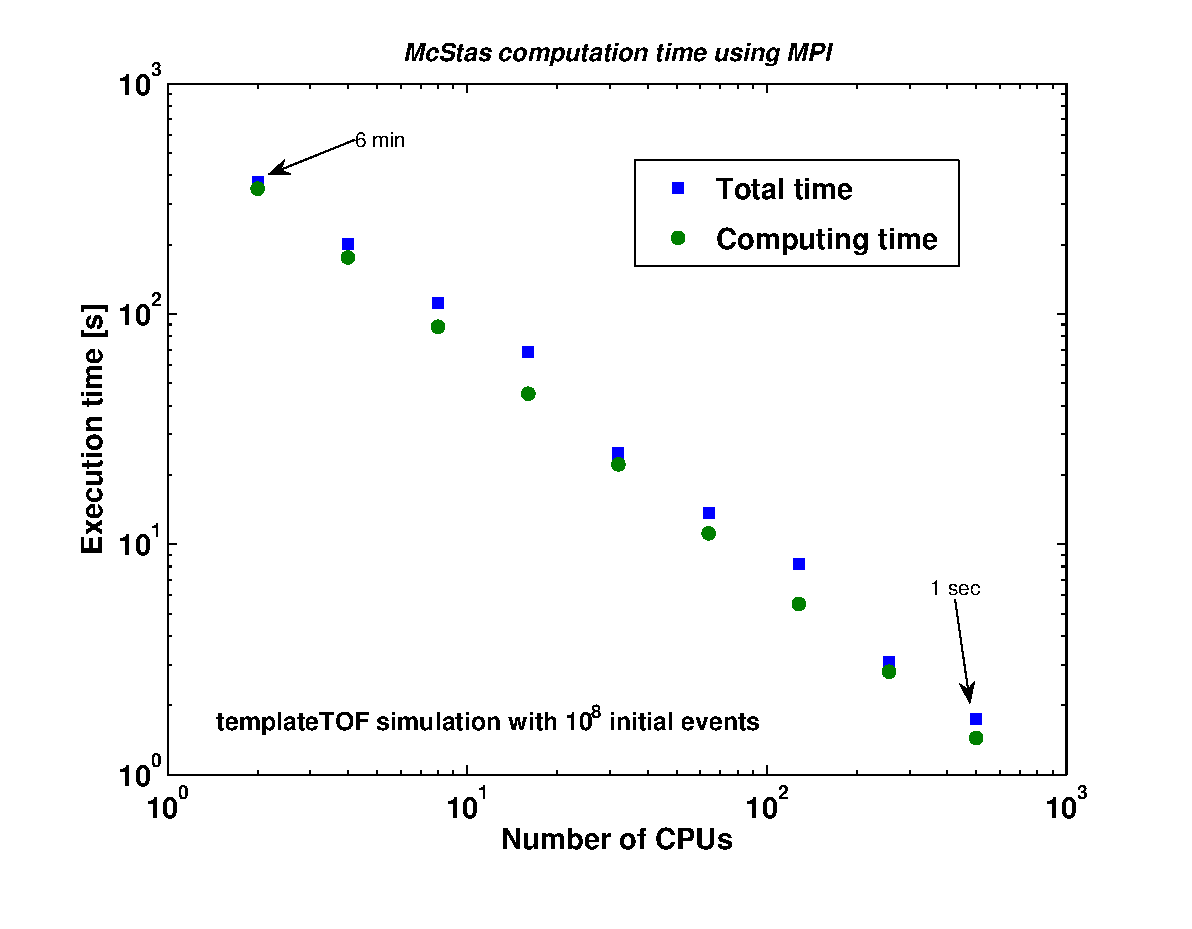
\includegraphics[width=0.55\textwidth]{figures/mpi_efficiency}
  \end{center}
  \caption{\MCS/MPI execution time as a function of computing nodes, with
   \textit{templateTOF} instrument and 1e8 initial neutron events. Tests performed on
    Lonestar@TACC (US Teragrid, 2008).}
\label{fig:mpi_efficiency}
\end{figure}

%-------------------------------------------------------------------------------
\subsection{MPI and Grid Bugs and limitations}
\index{MPI!limitations}
\index{Bugs!MPI and grid}

\begin{itemize}
\item Some header of output files might contain minor errors.
\item The computation split does not take into account the speed or the
  load of nodes: the overall time of a distributed computation is
  forced by the slowest node; for optimal performance, the ``cluster''
  should be homogeneous.
\item Interacting with a running simulation (USR1 and USR2 signals) is disabled
  with MPI.
\end{itemize}

%%% Local Variables:
%%% mode: latex
%%% TeX-master: "manual"
%%% End:

% Emacs settings: -*-mode: latex; TeX-master: "manual.tex"; -*-

\chapter{The \MCS kernel and meta-language}
\label{c:kernel}
\index{Kernel|(textbf}
\index{Meta-language}

Instrument definitions are written in a special \MCS meta-language which
is translated automatically by the compiler \mcs into a C program
which is in turn compiled to an executable that
performs the simulation. The meta-language is custom-designed for neutron
scattering and serves two main purposes: (i) to specify the interaction of a
single neutron ray with a single optical component, and (ii) to build a
simulation by constructing a complete instrument from individual
components.

For maximum flexibility and efficiency, the meta-language is based on C.
Instrument geometry, propagation of neutrons between the different
components, parameters, data input/output etc.\ is handled in the
meta-language and by the compiler \mcs. Complex calculations are written in
C embedded in the meta-language description of the
components. However, it is
possible to set up an instrument from existing components and
run a simulation without writing a single line of C code, working
entirely in the meta-language.

Apart from the meta-language, \MCS also includes a number of C library
functions and definitions that are useful for neutron ray-tracing
simulations. The definitions available for component developers are
listed in appendix~\ref{c:kernelcalls}. The list includes functions
for
\begin{itemize}
\item Computing the intersection between a flight-path and various
  objects (such as planes, cylinders, boxes and spheres)
\item Functions for generating random numbers
with various distributions
\item Functions for reading or writing information from/to data
  files
\item Convenient conversion factors between relevant units, etc.
\index{Library!run-time}
\index{Library!components!share}
\end{itemize}

The \MCS meta-language was designed to be readable, with a verbose
syntax and explicit mentioning of otherwise implicit information. The
recommended way to get started with the meta-language is to start by
looking at the examples supplied with \MCS, modifying them as necessary
for the application at hand.

%%%%%%%%%%%%%%%%%%%%%%%%%%%%%%%%%%%%%%%%%%%%%%%%%%%%%%%%%%%%%%%%%%%%%%%%%%%%%%%%
\section{Notational conventions}

Simulations generated by \MCS use a semi-classical description of the neutron
rays to compute the neutron trajectory through the instrument and its
interaction with the different components. The effect of gravity is taken into
account either in particular components (e.g. \verb+Guide_gravity+), or more
generally when setting an execution flag (\verb+-g+) to perform gravitation
computation. This latter setting is only an approximation and may produce wrong
results with some components.\index{Gravitation}

An instrument consists of a list of components through which the neutron
ray passes one after the other. The order of components is thus significant
since \mcs does not automatically check which component is the next to
interact with the neutron ray at a given point in the simulation. Note
that in case of a negative propagation time from one component to the
next, the neutron ray is by default \emph{absorbed} as this is often
an indication of unphysical conditions.

\index{Coordinate!system}
The instrument is given a global, absolute coordinate system. In
addition, every component in the instrument has its own local coordinate
system that can be given any desired position and orientation (though
the position and orientation must remain fixed for the duration of a
single simulation). 
By convention, the $z$ axis points in the direction of the beam, the $x$ axis
is perpendicular to the beam in the horizontal plane pointing left as seen
from the source, and the $y$ axis points upwards (see figure~\ref{f:axis}).
Nothing in the \MCS metalanguage enforces this convention, but if every component used
different conventions the user would be faced with a severe headache! It is
therefore necessary that this convention is followed by users implementing
new components.
\begin{figure}
  \begin{center}
    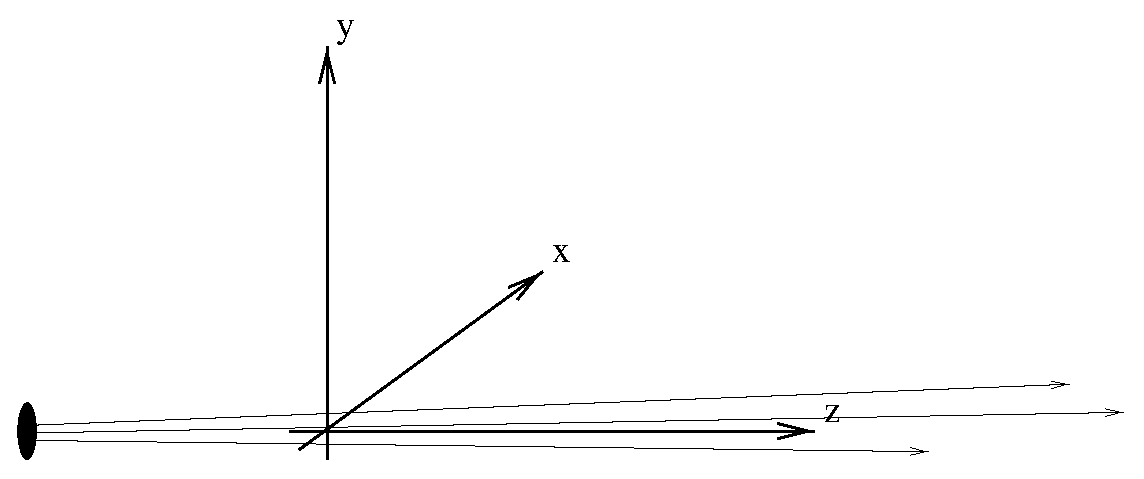
\includegraphics[width=0.8\textwidth]{figures/axis-conventions}
  \end{center}
\caption{conventions for the orientations of the axes in simulations.}
\label{f:axis}
\end{figure}

\index{Instrument definition!units|textbf}
\index{Units|textbf}
In the instrument definitions, units of length (\textit{e.g}.\ component
positions) are given in meters and units of angles (\textit{e.g}.\
rotations) are given in degrees.

\index{Neutron!state (position, velocity, time, spin, weight)|textbf}
The state of the neutron is given by
its position $(x,y,z)$ in meters, its velocity $(v_x, v_y, v_z)$ in
meters per second, the time $t$ in seconds, and the three spin parameters
$\left( s_x, s_y, s_z \right)$, and finally the neutron weight $p$ described in \ref{s:MCtechniques}.

%%%%%%%%%%%%%%%%%%%%%%%%%%%%%%%%%%%%%%%%%%%%%%%%%%%%%%%%%%%%%%%%%%%%%%%%%%%%%%%%
\section{Syntactical conventions}
\label{s:syntax}

Comments follow the C and C++ syntax

\begin{mcstas}
/* C style comment  */  
// C++ style comment
\end{mcstas}

\index{Comments}

%For backward-compatibility
%with early versions, comments may also be written as a percentage sign
%followed by a space (``\verb*+% ...+''), but this is not recommended and
%will be removed in a future version.

Keywords are not case-sensitive, for example ``\verb+DEFINE+'',
``\verb+define+'', and ``\verb+dEfInE+'' are all equivalent. However, by
convention we always write keywords in uppercase to distinguish them
from identifiers and C language keywords. In contrast, \MCS
identifiers (names), like C identifiers and keywords, \emph{are} case
sensitive, another good reason to use a consistent case convention for
keywords. All \MCS keywords are reserved, and thus should not be used
as C variable names. The list of these reserved keywords is shown in table~\ref{t:keywords}.

\begin{table}
  \begin{center}
    {\let\my=\\
    \begin{tabular}{|l|c|p{0.7\textwidth}|}
      \hline
      \texttt{Keyword} & Scope & Meaning \\
      \hline
      \texttt{ABSOLUTE} & I & Indicates that the AT and ROTATED keywords are in the absolute coordinate system. \\
      \texttt{AT} & I & Indicates the position of a component in an instrument definition. \\
      \texttt{COPY}& I,C & copy/duplicate an instance or a component definition. \\
      \texttt{DECLARE} & I,C & Declares C internal variables. \\
      \texttt{DEFINE} & I,C & Starts an INSTRUMENT or COMPONENT definition. \\
      \texttt{DEFINITION} & C & Defines component parameters that are constants (\#define). \\
      \texttt{DEPENDENCY} & C,I & Indicates any library dependency required to create the instrument. \\
      \texttt{END} & I,C & Ends the instrument or component definition. \\
      \texttt{SPLIT} & I & Enhance incoming statistics by event repetition. \\
      \texttt{EXTEND} & I & Extends a component TRACE section (plug-in). \\
      \texttt{FINALLY} & I,C & Embeds C code to execute when simulation ends. \\
      \texttt{GROUP} & I & Defines an exclusive group of components. \\
      \texttt{\%include} & I,C & Imports an instrument part, a component or a piece of C code (when within embedded C). \\
      \texttt{JUMP} & I & Iterative (loops) and conditional jumps. \\
      \texttt{INITIALIZE} & I,C & Embeds C code to be executed when starting. \\
      \texttt{ITERATE} & I & Defines iteration counter for JUMP. \\
      \texttt{MCDISPLAY} & C & Embeds C code to display component geometry. \\
      \texttt{OUTPUT} & C & Defines internal variables to be public and protected symbols (usually all global variables and functions of DECLARE).\\
      \texttt{PARAMETERS} & C & Defines a class of component parameter (DEFINITION, SETTING). \\
      \texttt{PREVIOUS} & C & Refers to a previous component position/orientation.\\
      \texttt{RELATIVE} & I & Indicates that the AT and ROTATED keywords are relative to an other component. \\
      \texttt{REMOVABLE} & I & Indicates that this component will be removed when the instrument is inserted into an other one using the \texttt{\%include} keyword. \\
      \texttt{ROTATED} & I & Indicates the orientation of a component in an instrument definition. \\
      \texttt{SAVE} & I,C & Embedded C code to execute when saving data. \\
      \texttt{SETTING} & C & Defines component parameters that are
      variables. \\
      \texttt{SHARE} & C & Declares global functions and variables to be shared. \\
      \texttt{TRACE} & I,C & Defines the instrument as a the component sequence. \\
      \texttt{WHEN}  & I & Condition for component activation and JUMP.\\
      \hline
    \end{tabular}
    \caption{Reserved \MCS keywords.
    Scope is 'I' for instrument and 'C' for component definitions.
    \index{Keywords|textbf}}
    \label{t:keywords}
    }
  \end{center}
\end{table}

It is possible, and usual, to split the input instrument definition
across several different files. For example, if a component is not
explicitly defined in the instrument,
\mcs will search for a file containing the component definition in the
standard component library (as well as in the current directory and any
user-specified search directories, see section~\ref{s:files}). It is
also possible to explicitly include another file using a line of the
form \indexKW{\%include}
\begin{lstlisting}
    %include "file"
\end{lstlisting}
Beware of possible confusion with the C language ``\verb+#include+''
statement, especially when it is used in C code embedded within the
\MCS meta-language. Files referenced with ``\verb+%include+'' are read
when the instrument is translated into C by \mcs, and must
contain valid \MCS meta-language input (and possibly C code). Files referenced with
``\verb+#include+'' are read when the C compiler generates an
executable from the generated C code, and must contain valid C.

Embedded C code is used in several instances in the \MCS
meta-language. Such code is copied by \mcs into the
generated simulation C program. Embedded C code is written by putting it
between the special symbols \%{ and \%}, as follows:
\begin{lstlisting}
%{ 
// Embedded C code...
%}
\end{lstlisting} 
\index{C code!embedded}
The \%\{ and \%\} must appear on a line by themselves (do not add comments after).
Additionally, if a ``\verb+%include+'' statement is found \emph{within} an embedded C code block, the specified file will be included from the 'share' directory of the standard component library \index{Library!components!share} (or from the
current directory and any user-specified search directories) as a C library, just like the usual ``\verb+#include+'' \emph{but only once}. For instance, if many components require to read data from a file, they may all ask for ``\verb+%include "read_table-lib"+'' \index{Library!read\_table-lib} without duplicating the code of this library. If the file has no extension, both \verb+.h+ and \verb+.c+ files will be searched and included, otherwise, only the specified file will be imported. The \MCS 'run-time' shared
library is included by default (equivalent to ``\verb+%include "mcstas-r"+'' in the \texttt{DECLARE} section). \index{Library!run-time}
For an
example of \texttt{\%include}, see the monitors/Monitor\_nD component. See also section \ref{s:instrdefs-extend} for insertion of full instruments in instruments (instrument concatenation).

If the instrument description compilation fails, check that the
keywords syntax is correct, that no semi-colon (\verb+;+) sign is
missing (e.g. in C blocks and after an ABSORB macro),
\indexMCRH{ABSORB}{}
and there are no name conflicts between instrument and component instances variables.\index{Compilation!failure}


%%%%%%%%%%%%%%%%%%%%%%%%%%%%%%%%%%%%%%%%%%%%%%%%%%%%%%%%%%%%%%%%%%%%%%%%%%%%%%%%
\section{Writing instrument definitions}
\label{s:instrdefs}
\index{Instrument definition}

The purpose of the instrument definition is to specify a sequence of
components, along with their position and parameters, which together
make up an instrument. Each component is given its own local coordinate
system, the position and orientation of which may be specified by its
translation and rotation relative to another component. An example is
given in section~\ref{s:Samples_vanadium.instr} and some additional
examples of instrument definitions can be found on the \MCS
web-page~\cite{mcstas_webpage} and in the \texttt{example} directory.

As a summary, the usual grammar for instrument descriptions is
\begin{mcstas}
DEFINE INSTRUMENT name(parameters)
DECLARE C_code
INITIALIZE C_code
TRACE components
{FINALLY C_code}
END
\end{mcstas}


%-------------------------------------------------------------------------------
\subsection{The instrument definition head}

\begin{mcstas}
DEFINE INSTRUMENT name (a_1, a_2, ...)
\end{mcstas} 
\indexKW{DEFINE INSTRUMENT}

This marks the beginning of the definition. It also gives the name of
the instrument and the list of instrument parameters. Instrument
parameters describe the configuration of the instrument, and usually
correspond to setting parameters of the components, see section \ref{s:compdefs}. A motor position is
a typical example of an instrument parameter. The input parameters of
the instrument constitute the input that the user (or possibly a
front-end program) must supply when the
generated simulation is started.

\index{Parameters!Instruments}
By default, the parameters will be floating point numbers, and will have
the C type \verb+double+ (double precision floating point). The type of
each parameter may optionally be declared to be \verb+int+ for the C
integer type or \verb+char *+ for the C string type. The name
\verb+string+ may be used as a synonym for \verb+char *+, and floating
point parameters may be explicitly declared using the name
\verb+double+. The following example illustrates all possibilities:
\begin{mcstas}
DEFINE INSTRUMENT test(d1, double d2, int i, char *s1, string s2)
\end{mcstas}

Here \verb+d1+ and \verb+d2+ will be floating point parameters of C type
\verb+double+, \verb+i+ will be an integer parameter of C type \verb+int+, and
\verb+s1+ and \verb+s2+ will be string parameters of C type \verb+char *+.
\index{Parameters!optional, default value} The parameters of an instrument may
be given default values. Parameters with default values are called
\emph{optional parameters}, and need not be given an explicit value when the
instrument simulation is executed. When executed without any parameter value in
the command line (see section~\ref{s:run-sim}), the instrument asks for all
parameter values, but pressing the \verb+Return+ key selects the default value
(if any). When used with at least one parameter value in the command line, all
non specified parameters will have their value set to the default one (if
any). A parameter is given a default value using the syntax
``\textit{param}\texttt{= }\textit{value}''.  For example
\begin{mcstas}
DEFINE INSTRUMENT test(d1= 1, string s2="hello")
\end{mcstas}
Here \verb+d1+ and \verb+d2+ are optional parameters and if no
value are given explicitly, ``1'' and ``hello'' will be used.

Optional parameters can greatly increase the convenience for users of
instruments for which some parameters are seldom changed or of unclear
signification to the user. Also, if all instrument parameters have default
values, then the simple command \verb+mcdisplay+ \verb+test.instr+ will show the
instrument view without requesting any other input, which is usually a good
starting point to study the instrument design.

%-------------------------------------------------------------------------------
\subsection{The \texttt{DEPENDENCY} line}
\indexKW{DEPENDENCY}
\label{s:dependency}
\begin{mcstas}
DEPENDENCY "-lLIB1 -lLIB2 .."
\end{mcstas}

If you make use of external library calls in your instrument, you may indicate 
the dependency list to be used for the compilation of the instrument, as a single 
DEPENDENCY keyword and a string argument, all on a single line such as:
\begin{mcstas}
DEPENDENCY "-lgsl -lgslcblas"
\end{mcstas}
The concatenation of all found dependencies from the instrument, but also from 
all used components, will be printed to the terminal (stdout) as
\begin{mcstas}
CFLAGS=-lgsl -lgslcblas
\end{mcstas}
This line is interpreted by \verb+mcrun+ (see section \ref{s:mcrun}) and passed 
to the compiler. It must be indicated just before the \texttt{DECLARE} section.
This line is optional, and if omitted you may need to manually link the instrument with the libraries and add the proper library names to the MCSTAS\_CFLAGS or CFLAGS environment variables.

%-------------------------------------------------------------------------------
\subsection{The \texttt{DECLARE} section}
\indexKW{DECLARE}
\label{s:declare}

\begin{mcstas}
DECLARE
%{ 
   // C declarations of global variables etc. ...
%}
\end{mcstas} 
\index{C code!embedded}
 This gives C declarations that may be
referred to in the rest of the instrument definition. A typical use is to
declare global variables or small functions that are used elsewhere in the
instrument. The \verb+%include ''file''+ keyword may be used to import a
specific
component definition or a part of an instrument. Variables defined here are
global, and may conflict with internal \MCS variables, specially symbols like
\verb+x,y,z,sx,sy,sz,vx,vy,vz,t+ and generally all names starting with \verb+mc+
should be avoided. If you can not compile the instrument, this may be the
reason. \index{Compilation!failure}The \texttt{DECLARE} section is optional.

%-------------------------------------------------------------------------------
\subsection{The \texttt{INITIALIZE} section}
\indexKW{INITIALIZE}
\label{s:initialize}

\begin{mcstas}
INITIALIZE
%{
// C initializations. 
%}
\end{mcstas} 
\index{C code!embedded}
This gives code that is executed when the
simulation starts. This section is optional. Instrument setting parameters may
be modified in this section (e.g. doing tests or automatic settings).

%-------------------------------------------------------------------------------
\subsection{The \texttt{NEXUS} extension}
\index{NeXus!extension}
\index{Data formats}
\label{s:nexus}

The NeXus format~\cite{nexus_webpage} requires to link the simulation to
additional libraries (HDF and NeXus) which must have been
pre-installed. Preferably, \MCS should have been installed with the
\verb+./configure --with-nexus+ on Unix/Linux systems. To activate the NeXus
output, the compilation of the instrument must be done with flag
\verb+-DUSE_NEXUS+ \verb+-lNeXus+.
The resulting executable is no longer portable.

The default NeXus format is HDF5 with compression. 

You may choose the name of the output file with the \verb+-f filename+ option
from the instrument executable or \verb+mcrun+ (see Sections \ref{s:run-sim},
\ref{s:mcrun} and Table \ref{f:simoptions2}).

Then, the output format is chosen as usual with the \verb+--format=NeXus+ option
when launching the simulation. All output files are stored in the output
 \textit{filename},
as well as the instrument description itself. Other formats are
still available. When run on a distributed system (e.g. MPI), detectors are
gathered, but list of events (see e.g. component Virtual\_output) are stored as
one data set per node.

%-------------------------------------------------------------------------------
\subsection{The \texttt{TRACE} section}
\indexKW{TRACE}
\label{s:trace}


As a summary, the usual grammar for component instances within the instrument
TRACE section is
\begin{mcstas}
COMPONENT name = comp(parameters)
  AT (...) [RELATIVE [reference|PREVIOUS] | ABSOLUTE]
 {ROTATED  {RELATIVE [reference|PREVIOUS] | ABSOLUTE} }
\end{mcstas}

The \texttt{TRACE} keyword starts a section giving the list of
components that constitute the instrument.
Components are declared like this:
\begin{mcstas}
COMPONENT name = comp(p_1 = e_1, p_2 = e_2, ...)
\end{mcstas}
\index{Component!declaration (\texttt{TRACE})}
\indexKW{COMPONENT}
\index{Parameters!setting}
\index{Parameters!definition}
This declares a component named \textit{name} that is an instance of the
component definition named \textit{comp}. The parameter list gives the
setting and definition parameters for the component. The expressions $e_1,
e_2, \ldots$ define the values of the parameters. For setting parameters
arbitrary ISO-C expressions may be used, while for definition parameters
only \emph{constant} numbers, strings, names of instrument parameters, or names
of C identifiers are allowed (see section~\ref{s:comp-header} for details of
the difference between definition and setting parameters). To assign the
value of a general expression to a definition parameter, it is necessary to
declare a variable in the \texttt{DECLARE} section, assign the value to the
variable in the \texttt{INITIALIZE} section, and use the variable as the
value for the parameter.

The \MCS program takes care to rename parameters appropriately in the
output so that no conflicts occur between different component
definitions or between component and instrument definitions. It is thus
possible (and usual) to use a component definition multiple times
in an instrument description.

Beware about variable type conversion when setting numerical parameter values, as in \verb+p1=12/1000+. In this example, the parameter \verb+p1+ will be set to 0 as the division of the two integers is indeed 0. To avoid that, use explicitly floating type numbers as in \verb+p1=12.0/1000+.\index{Bugs!integer versus floating-point division}

The compiler \mcs will automatically search for a file containing a
definition of the component if it has not been declared previously. The
definition is searched for in a file called ``\textit{name\/}\texttt{.comp}''. See
section~\ref{s:files} for details on which directories are searched. This
facility is often used to refer to existing component definitions in
standard component libraries. It is also possible to write component
definitions in the main file before the instrument definitions, or to
explicitly read definitions from other files using \verb+%include+
(not within embedded C blocks).

The physical position of a component is specified using an \texttt{AT} modifier
following the component declaration:
\indexKW{AT}
\indexKW{RELATIVE}
\indexKW{ABSOLUTE}
\begin{mcstas}
  AT (x,y,z) RELATIVE name
\end{mcstas}
This places the component at position $(x,y,z)$ in the coordinate system
of the previously declared component \textit{name}. Placement may also
be absolute (not relative to any component) by writing
\begin{mcstas}
  AT (x,y,z) RELATIVE ABSOLUTE
\end{mcstas}
Any C expression may be used for $x$, $y$, and $z$. The \texttt{AT}
modifier is required.
Rotation is achieved similarly by writing
\indexKW{ROTATED}
\begin{mcstas}
  ROTATED (phi_x,phi_y,phi_z) RELATIVE name
\end{mcstas}
This will result in a coordinate system that is rotated first the angle $\phi_x$
(in degrees) around the $x$ axis, then $\phi_y$ around the $y$ axis, and finally
$\phi_z$ around the $z$ axis. Rotation may also be specified using
\texttt{ABSOLUTE} rather than \texttt{RELATIVE}. If no rotation is specified,
the default is $(0,0,0)$ using the same relative or absolute specification used
in the \texttt{AT} modifier. We \emph{strongly} recommend to apply all rotations
of an instrument description on Arm class components only, acting as
goniometers, and position the optics on top of these. This usually makes it much
easier to orient pieces of the instrument, and avoid positioning errors.

The \emph{position} of
a component is actually the origin of its local coordinate
system. Usually, this is used as the input window position (e.g. for
guide-like components), or the center position for
cylindrical/spherical components.

The \texttt{PREVIOUS}
\indexKW{PREVIOUS}
keyword is a generic name to
refer to the previous component in the simulation. Moreover, the
\texttt{PREVIOUS(n)} keyword will refer to the $n$-th previous component,
starting from the current component, so that \texttt{PREVIOUS} is equivalent to
\texttt{PREVIOUS(1)}. This keyword should be used after the \texttt{RELATIVE}
keyword, but not for the first component instance of the instrument description.
\begin{mcstas}
AT (x,y,z) RELATIVE PREVIOUS
ROTATED (phi_x, phi_y, phi_z) RELATIVE PREVIOUS(2)
\end{mcstas}
Invalid \texttt{PREVIOUS} references will be assumed to be absolute placement.

The order and position of components in the \texttt{TRACE} section does not
allow components to overlap, except for particular cases (see the \texttt{GROUP}
keyword below).  Indeed, many components of the \MCS library
\index{Library!components} start by propagating the neutron event to the
beginning of the component itself.  Anyway, when the corresponding propagation
time is found to be negative (\textit{i.e.} the neutron ray is already \emph{after}
or \emph{aside} the component, and has thus passed the 'active' position), the
neutron event is ABSORBed,
\indexMCRH{ABSORB}{}
resulting in a zero intensity and event counts after
a given position. The number of such removed neutrons is indicated at the end of
the simulation.  Getting such warning messages is an indication that either some
components overlap, or some neutrons are getting outside of the simulation, for
instance this usually happens after a monochromator, as the non-reflected beam
is indeed lost. A special warning appears when no neutron ray has reached some
part of the simulation. This is usually the sign of either overlapping
components or a very low intensity.\index{Absorption}\index{Neutron!absorption}

For experienced users, we recommend as well the usage of the \texttt{WHEN} and
\texttt{EXTEND} keywords, as well as other syntax extensions presented in
section \ref{s:instrdefs-extend} below.

%-------------------------------------------------------------------------------
\subsection{The \texttt{SAVE} section}
\indexKW{SAVE}
\label{s:save}

\begin{mcstas}
SAVE 
%{
  // C code to execute each time a temporary save is required...
%}
\end{mcstas} 

\indexSIG{USR2}{textbf}
This gives code that will be
executed when the simulation is requested to save data, for instance when
receiving a USR2 signal (on Unix systems), or using the \verb+Progress_bar+
component with intermediate savings. It is also executed when the simulation
ends. This section is optional.

%-------------------------------------------------------------------------------
\subsection{The \texttt{FINALLY} section}
\indexKW{FINALLY}
\label{s:finally}

\begin{mcstas}
FINALLY
%{
   // C code to execute at end of simulation
%}
\end{mcstas}
\indexSIG{TERM}{textbf}
\indexSIG{INT}{textbf}
This gives code that will be executed when the simulation has
ended. When existing, the \texttt{SAVE} section is first executed. The
\texttt{FINALLY} section is optional.
A simulation may be requested to end before all neutrons have been
traced when receiving a TERM or INT signal (on Unix systems), or with
Control-C, causing code in \texttt{FINALLY} to be evaluated.


%-------------------------------------------------------------------------------
\subsection{The end of the instrument definition}
\label{s:end}
\indexKW{END}

The end of the instrument definition must be explicitly marked using the keyword
\begin{lstlisting}
END
\end{lstlisting}

\subsection{Code for the instrument \texttt{vanadium\_example.instr}}
\label{s:Samples_vanadium.instr}
A commented instrument definition taken from the \texttt{examples} directory is
here shown as an example of the use of \MCS.
%FIXME \smallverbatimfile{McCode/mcstas-comps/examples/Samples_vanadium.instr}



%%%%%%%%%%%%%%%%%%%%%%%%%%%%%%%%%%%%%%%%%%%%%%%%%%%%%%%%%%%%%%%%%%%%%%%%%%%%%%%%
\section{Writing instrument definitions - complex arrangements and syntax}
\label{s:instrdefs-extend}
\index{Instrument definition}

In this section, we describe some additional ways to build instruments using
groups, code extension, conditions, loops and duplication of components.

As a summary, the nearly complete grammar definition for component instances
within the instrument TRACE section is:

\begin{mcstas}
{SPLIT} COMPONENT name = comp(parameters) {WHEN condition}
  AT (...) [RELATIVE [reference|PREVIOUS] | ABSOLUTE]
  {ROTATED {RELATIVE [reference|PREVIOUS] | ABSOLUTE} }
  {GROUP group_name}
  {EXTEND C_code}
  {JUMP [reference|PREVIOUS|MYSELF|NEXT] [ITERATE number_of_times | WHEN condition] }
\end{mcstas}

%-------------------------------------------------------------------------------
\subsection{Embedding instruments in instruments TRACE}
\indexKW{\%include}
\label{s:instrdefs-include-instr}
The \texttt{\%include} insertion mechanism may be used within the TRACE section,
in order to concatenate instruments together. This way, each DECLARE,
INITIALIZE, SAVE, and FINALLY C blocks, as well as instrument parameters from
each part are concatenated. The TRACE section is made of inserted COMPONENTS
from each part. In principle, it is then possible to write an instrument as:
\begin{mcstas}
DEFINE concatenated()
TRACE

%include "part1.instr"
%include "part2.instr"

END
\end{mcstas}
where each inserted instrument is a valid full instrument. In order to avoid
some components to be duplicated - e.g. Sources from each part - a special
syntax in the TRACE section
\begin{mcstas}
REMOVABLE COMPONENT a=...
\end{mcstas}
marks the component \textit{a} as removable when inserted. In principle, inserted
instruments may themselves use \texttt{\%include}.

%-------------------------------------------------------------------------------
\subsection{Groups and component extensions - GROUP - EXTEND}
\indexKW{GROUP}
\indexKW{EXTEND}
\label{s:instrdefs-extend-group}

It is sometimes desirable to slightly modify an existing component of the \MCS library. One would usually make a copy of the component, and extend the code of its \texttt{TRACE} section. \MCS provides an easy way to change the behavior of existing components in an instrument definition without duplicating files, using the \texttt{EXTEND} modifier
\indexKW{EXTEND}
\begin{mcstas}
EXTEND
%{ 
// C code executed after the component TRACE section...
%}
\end{mcstas} 
\index{C code!embedded}
The embedded C code is appended to the
component \texttt{TRACE} section, and all its internal variables (as well as all
the \texttt{DECLARE} instrument variables, \emph{except} instrument parameters)
may be used. To use instrument parameters, you should copy them into global
variables in the DECLARE instrument section, and refer to these latter.  This
component declaration modifier is of course optional. You will find numerous
usage examples, and in particular in the Sources section of the Component
manual.

In some peculiar configurations it is necessary to position one or more groups
of components, nested, in parallel, or overlapping. One example is a multiple
crystal monochromator. One would then like the neutron ray to interact with
\emph{one of} the components of the group and then continue.

In order to handle such arrangements without removing neutrons, groups are
defined by the \texttt{GROUP} modifier (after the AT-ROTATED positioning):
\begin{mcstas}
GROUP name
\end{mcstas}
to all involved component declarations.
\indexKW{GROUP}
All components of
the same named group are tested one after the other, until one of them interacts
(uses the SCATTER macro\indexMCRH{SCATTER}{}). The selected component
acts on the neutron ray, and the rest of the group is skipped. Such groups are
thus exclusive (only one of the elements is active).

Within a \texttt{GROUP}, \emph{all} \texttt{EXTEND} sections of the group are
executed. In order to discriminate components that are active from those that
are skipped, one may use the SCATTERED flag, which is set to zero when entering
each component or group, and incremented when the neutron is SCATTERed, as in
the following example
\indexMCCH{SCATTERED}{}
\begin{mcstas}
COMPONENT name0 = comp (
                  p_1 = e_1, 
                  p_2 = e_2, 
                  ...)
AT (0,0,0) ABSOLUTE

COMPONENT name1 = comp... 
AT (...) ROTATED (...)

GROUP GroupName EXTEND
%{ 
   if (SCATTERED) printf("I scatter"); else printf("I do not scatter");
%}

COMPONENT} name2 = comp ...
AT (...) ROTATED (...)
GROUP GroupName
\end{mcstas}
Components \emph{name1} and \emph{name2} are at the same position. If the first
one intercepts the neutron
(and has a SCATTER\indexMCRH{SCATTER}{}
within its \texttt{TRACE}
section), the SCATTERED\indexMCCH{SCATTERED}{}
variable becomes true, the code extension will result in
printing "I scatter", and the second component will be skipped.  Thus, we
recommend to make use of the SCATTER keyword each time a component 'uses' the
neutron (scatters, detects, \ldots) within component definitions (see section
\ref{s:compdefs}). Also, the components to be grouped should be consecutive in
the TRACE section of the instrument, and the GROUPed section should not contain
components which are not part of the group.

A usage example of the GROUP keyword can be found in the \\
\verb+Neutron site/ILL/ILL_H15_IN6+ instrument from the \verb+mcgui+, to model 3 monochromators.

Combining EXTEND, GROUP and WHEN can result in unexpected behavior. Please read the related warning at the end of section \ref{s:instrdefs-extend-when}.

%-------------------------------------------------------------------------------
\subsection{Duplication of component instances - COPY}
\indexKW{COPY}
\label{s:instrdefs-extend-copy}

Often, one has a set of similar component instances in an instrument. These
could be e.g. a set of identical monochromator blades, or a set of detectors or
guide elements.  Together with JUMPs (see below), there is a way to copy a
component instance, duplicating parameter set.

Position (AT) and rotation (ROTATED) specification must
be explicitly entered in order to avoid component overlapping, and it
is futher recommended to explicitly set any EXTEND, GROUP, JUMP and
WHEN keyword to each \emph{mother} or copied instance. But \textbf{BEWARE},
advanced combinations of (many) keywords \emph{may} introduce
unexpected behaviour.

The syntax for instance copy is
\begin{mcstas}
COMPONENT name = COPY (instance_name)
\end{mcstas}
where \textit{instance\_name} is the name of a preceding component instance in the
instrument. It may be 'PREVIOUS' as well.

If you would like to change only some of the parameters in the instance copy, you may write, e.g.:

\begin{mcstas}
COMPONENT name = COPY (instance_name)(par1=0, par2=1)
\end{mcstas}

which will override the original instance parameter values. This possibility to
override parameters is very useful in case of describing e.g. sample environments
using the Isotropic\_Sqw and PowderN components, which allow \emph{concentric}
geometry (first instance must have \verb+concentric = 1+ and the second
\verb+concentric = 0+). In case EXTEND, GROUP, JUMP and WHEN keywords are
defined for the copied instance, these will override the settings from the
copied instance.


In the case where there are many duplicated components all originating from the
same instance, there is a mechanism for automating copied instance names:
\begin{mcstas}
COMPONENT COPY(root_name) = COPY(instance_name)
\end{mcstas}
will concatenate a unique number to \textit{root\_name}, avoiding name
conflicts. As a side effect, referring to this component instance (for
e.g. further positioning) is not straight forward as the name is determined by
\mcs and does not depend completely on the user's choice, even though the
PREVIOUS keyword may still be used. We thus recommend to use this naming
mechanism only for components which should not be referred to in the instrument.

This automatic naming may be used anywhere in the TRACE section of the
instrument, so that all components which do not need further referring may be
labeled as COPY(Origin).

As an example, we show how to build a guide made of equivalent elements. Only
the first instance of the Guide component is defined, whereas following
instances are copies of that definition. The instance name of Guide components
is set automatically.

\begin{mcstas}
COMPONENT CG_In = Arm() AT (...)

COMPONENT CG_1  = Guide_gravity(l=L/n, m=1, ...)
  AT (0,0,0) RELATIVE PREVIOUS

COMPONENT COPY(CG_1)  = COPY(CG_1)
  AT (0,0,L/n+d) RELATIVE PREVIOUS
  ROTATED (0, (L/n+d)/R*180/PI, 0) RELATIVE PREVIOUS

COMPONENT COPY(CG_1)  = COPY(CG_1)
  AT (0,0,L/n+d) RELATIVE PREVIOUS
  ROTATED (0, (L/n+d)/R*180/PI, 0) RELATIVE PREVIOUS
...
COMPONENT CG_Out = Arm() AT (0,0,L/n) RELATIVE PREVIOUS
\end{mcstas}

%-------------------------------------------------------------------------------
\subsection{Conditional components - WHEN}
\indexKW{WHEN}
\label{s:instrdefs-extend-when}

One of the most useful features of the extended \MCS syntax is the conditional
\texttt{WHEN} modifier. This optional keyword comes before the AT-ROTATED
positioning. It basically enables the component only when a given condition is
true (non null).

\begin{mcstas}
  COMPONENT name = comp (p_1 = e_1, p_2 = e_2, ...)
  WHEN condition
\end{mcstas}
The condition has the same scope as the EXTEND modifier, i.e. may use component
internal variables as well as all the \texttt{DECLARE} instrument variables.

Usage examples could be to have specific monitors only sensitive to selected
processes, or to have components which are only present under given
circumstances (e.g. removable guide or radial collimator), or to select a sample
among a set of choices.

In the following example, an EXTEND block sets a condition when a scattering
event is encountered, and the following monitor is then activated.
\begin{mcstas}
COMPONENT Sample = V_sample(...) AT ...
  EXTEND
  %{
    if (SCATTERED) flag=1; else flag=0;
  %}

COMPONENT MyMon = Monitor(...) WHEN (flag==1)
  AT ...
\end{mcstas}
\indexMCCH{SCATTERED}{}

The WHEN keyword only applies to the TRACE section and related EXTEND blocks of
instruments/components. Other sections (INITIALIZE, SAVE, MCDISPLAY, FINALLY)
are executed independently of the condition. As a side effect, the 3D view of
the instrument (mcdisplay) will show all components as if all conditions were
true.

Also, the \verb+WHEN+ keyword is a condition for \verb+GROUP+. This means that
when the \verb+WHEN+ is false, the component instance is not active in the
\verb+GROUP+ it belongs to.\index{Bugs!WHEN vs GROUP}

A usage example of the WHEN keyword can be found in the \\
\verb+Neutron site/ILL/ILL_TOF_Env+ instrument from the \verb+mcgui+, to monitor
neutrons depending on their fate.


\textbf{WARNING:} Combining WHEN, EXTEND and GROUP can result in unexpected behavior,
please use with caution! Let for instance a GROUP of components all have the
same WHEN condition, i.e. if the WHEN condition is false, none of the elements
SCATTER, meaning that all neutrons will be ABSORBed.
\indexMCRH{ABSORB}{}
\indexMCRH{SCATTER}{}
As a solution to this
problem, we propose to include an EXTENDed Arm component in the GROUP, but with
the opposite WHEN condition and a SCATTER keyword in the EXTEND section. This
means that when none of the other GROUP elements are present, the Arm will be
present and SCATTER.


%-------------------------------------------------------------------------------
\subsection{Component loops and non sequential propagation - JUMP}
\indexKW{JUMP}
\indexKW{ITERATE}
\indexKW{WHEN}
\label{s:instrdefs-extend-jump}

There are situations for which one would like to repeat a given component many
times, or under a given condition. The JUMP modifier is meant for that and
should be placed after the positioning, GROUP and EXTEND. This breaks the
sequential propagation along components in the instrument description. There may
be more than one JUMP per component instance.

The jump may depend on a condition:
\begin{mcstas}
COMPONENT name = comp(p_1 = e_1, p_2 = e_2, ...)
  AT (...)
  JUMP reference WHEN condition
\end{mcstas}

in which case the instrument TRACE will jump to the \textit{reference} when
\textit{condition} is true.

The \textit{reference} may be an instance name, as well as PREVIOUS, PREVIOUS($n$),
MYSELF, NEXT, and NEXT($n$), where $n$ is the index gap to the target either
backward (PREVIOUS) or forward (NEXT), so that PREVIOUS(1) is PREVIOUS and
NEXT(1) is NEXT. MYSELF means that the component will be iterated as long as the
condition is true. This may be a way to handle multiple scattering, if the
component has been designed for that.
\indexKW{PREVIOUS}
\indexKW{MYSELF}
\indexKW{NEXT}

The jump arrives directly inside the target component, in the local coordinate
system (i.e. without applying the AT and ROTATED keywords). In order to control
better the target positions, it is \emph{required} that, except for looping
MYSELF, the target component type should be an \emph{Arm}.
\indexKW{ROTATED}

There is a more general way to iterate components, which consists in repeating
the loop for a given number of times.
\begin{mcstas}
  JUMP reference ITERATE number_of_times
\end{mcstas}
This method is specially suited for very long curved guides of similar
components, but in order to take into account rotation and translation between
guide sections, the iterations are performed between Arm's.
\indexKW{ITERATE}

In the following example for a curved guide made on $n=500$ elements of length
$L$ on a curvature radius $R$, with gaps $d$ between elements, we simply write:
\begin{mcstas}
COMPONENT CG_In = Arm() AT (...)

COMPONENT CG_1  = Guide_gravity(l=L/n, m=1, ...)
  AT (0,0,0) RELATIVE PREVIOUS

COMPONENT CG_2_Position = Arm()
  AT (0,0,L/n+d) RELATIVE PREVIOUS
  ROTATED (0, (L/n+d)/R*180/PI, 0) RELATIVE PREVIOUS

COMPONENT CG_2  = Guide_gravity(l=L/n, m=1, ...)
  AT (0,0,0) RELATIVE PREVIOUS
  ROTATED (0, (L/n+d)/R*180/PI, 0) RELATIVE PREVIOUS
  JUMP CG_2_Position ITERATE n
...
COMPONENT CG_Out = Arm() AT (0,0,L/n) RELATIVE PREVIOUS
\end{mcstas}

Similarly to the \texttt{WHEN} modifier (see section
\ref{s:instrdefs-extend-when}), \texttt{JUMP} only applies within the TRACE
section of the instrument definition. Other sections (INITIALIZE, SAVE,
MCDISPLAY, FINALLY) are executed independently of the jump. As a side effect,
the 3D view of the instrument (mcdisplay) will show components as if there was
no jump. This means that in the following example, the very long guide 3D view
only shows a single guide element.

It is \emph{not} recommended to use the \verb+JUMP+ inside \verb+GROUP+s, as the
JUMP condition/counter applies to the component instance within its group.

We would like to emphasize the potential errors originating from such
jumps. Indeed, imbricating many jumps may lead to situations were it is
difficult to understand the flow of the simulation. We thus recommend the usage
of JUMPs only for experienced and cautious users.\index{Bugs!JUMPs}

%-------------------------------------------------------------------------------
\subsection{Enhancing statistics reaching components - SPLIT}
\indexKW{SPLIT}
\label{s:instrdefs-extend-enhance}

The following method applies when the incoming neutron event distribution is
considered to be representative of the real beam, but neutrons are lost in the
course of propagation (with low efficiency processes, absorption, etc). Then,
one may think that it's a pity to have so few events reaching the 'interesting'
part of the instrument (usually close to the end of the instrument description).
If some components make extensive use of random numbers (MC choices), they
shuffle this way the distributions, so that identical incoming events will not
produce the same outgoing event. In this case, you may use the \verb+SPLIT+
keyword with the syntax

\begin{mcstas}
  SPLIT r COMPONENT name = comp(...)
\end{mcstas}

where the optional number $r$ specifies the number of repetitions for each
event. Default is $r=10$.  Each neutron event reaching component \textit{name} will
be repeated $r$ times with a weight divided by $r$, so that in practice the
number of events for the remaining part of the simulation (down to the END),
will potentially have more statistics. This is only true if following components
(and preferably component \textit{name}) use random numbers. You may use this
method as many times as you wish in the same instrument, e.g. at the
monochromator and sample position. This keyword can also be used within a
GROUP. The efficiency is roughly $r$ raised to the number of occurrences in the
instrument, so that enhancing two components with the default $r=10$ will
produce at the end an enhancement effect of 100 in the number of events. The
execution time will usually get slightly longer. This technique is known as the
\emph{stratified sampling} (see Appendix \ref{s:MCtechniques}). If the
instrument makes use of global variables - e.g. in conjunction with a WHEN or
User Variable monitoring (see Monitor\_nD) - you should take care that these
variables are set properly for each SPLIT loop, which usually means that they
must be reset inside the SPLITed section and assigned/used further
on. \index{Bugs!SPLIT}

A usage example of the SPLIT keyword can be found in the \\
\verb+Neutron site/ILL/ILL_H15_IN6+ instrument from the \verb+mcgui+, to enhance
statistics for neutrons scattering on monochromators and sample.

%%%%%%%%%%%%%%%%%%%%%%%%%%%%%%%%%%%%%%%%%%%%%%%%%%%%%%%%%%%%%%%%%%%%%%%%%%%%%%%%
\section{Writing component definitions}
\label{s:compdefs}

The purpose of a \MCS component is to model the interaction of a
neutron with a physical component of a real instrument. Given the
state of the incoming neutron ray, the
component definition calculates the state of the neutron ray when it leaves
the component.  The calculation of the effect of the component on the
neutron is performed by a block of embedded C code.
One example of a component definition is given in section~\ref{s:slit}, and all
component definitions can be found on the \MCS
web-page~\cite{mcstas_webpage} and are described in the \MCS component manual.

There exists a large number of functions and constants available in
order to write efficient components. See appendix~\ref{c:kernelcalls}
for
\begin{itemize}
\item neutron propagation functions
\item geometric intersection time computations
\item mathematical functions
\item random number generation
\item physical constants
\item coordinate retrieval and operations
\item file generation routines (for monitors),
\item data file reading
\end{itemize}

%A component definition looks as follows:


%-------------------------------------------------------------------------------
\subsection{The component definition header}
\label{s:comp-header}

\begin{mcstas}
DEFINE COMPONENT name
\end{mcstas}
\indexKW{DEFINE COMPONENT}

This marks the beginning of the definition, and defines the name of the
component.
\begin{mcstas}
DEFINITION PARAMETERS (d_1, d_2, ...)
SETTING PARAMETERS (s_1, s_2, ...)
\end{mcstas}
\indexKW{DEFINITION PARAMETERS}
\indexKW{SETTING PARAMETERS}
This declares the definition and setting parameters of the component.
These parameters can be
accessed from all sections of the component (see below),
as well as in \verb+EXTEND+ sections of the instrument definition (see section~\ref{s:instrdefs}).
\index{Parameters!setting}
\index{Parameters!definition}

Setting parameters are translated into C variables usually of type
\verb+double+ in the generated simulation program, so they are usually
numbers. Definition parameters are translated into \verb+#define+ macro
definitions, and so can have any type, including strings, arrays, and
function pointers.

However, because of the use of \verb+#define+, definition parameters
suffer from the usual problems with C macro definitions. Also, it is not
possible to use a general C expression for the value of a definition
parameter in the instrument definition, only constants and variable
names may be used. For this reason, setting parameters should be used
whenever possible.

Outside the \verb+INITIALIZE+ section of components, changing setting parameter
values only affects the current section.

There are a few cases where the use of definition parameters instead of
setting parameters makes sense. If the parameter is not numeric, nor a character string ({\em i.e.} an
array, for example), a setting parameter cannot be
used. Also, because of the use of \verb+#define+, the C compiler can
treat definition parameters as constants when the simulation is
compiled. For example, if the array sizes of a multidetector are
definition parameters, the arrays can be statically allocated in the
component \verb+DECLARE+ section. If setting parameters were used, it
would be necessary to allocate the arrays dynamically using {\em e.g.}\
\verb+malloc()+.

Setting parameters may optionally be declared to be of type \verb+int+,
\verb+char *+ and \verb+string+, just as in the instrument definition (see
section~\ref{s:instrdefs}).

\begin{mcstas}
OUTPUT PARAMETERS (s_1, s_2, ...)
\end{mcstas}

\indexKW{OUTPUT PARAMETERS}
This declares a list of C identifiers (variables, functions) that are
output parameters (\textit{i.e.} global) for the
component. Output parameters are used to hold values that are computed
by the component itself, rather than being passed as input. This could
for example be a count of neutrons in a detector or a constant that is
precomputed to speed up computation.

Using \texttt{OUTPUT PARAMETERS} is \emph{strongly recommended} for
\texttt{DECLARE} and internal/global component variables and functions in order
to prevent that instances of the same component use the same variable
names. Moreover (see section \ref{s:comp-declare} below), these may be accessed
from any other instrument part (e.g. using the \verb+MC_GETPAR+ C macro).  On
the other hand, the variables from the SHARE sections should \emph{not} be
defined as OUTPUT parameters.

The \texttt{OUTPUT} \texttt{PARAMETERS} section is optional.

\subsubsection{Optional component parameters}
\index{Parameters!optional, default value}

Just as for instrument parameters, the definition and setting parameters of a
component may be given a default value. Parameters with default values are
called \emph{optional parameters}, and need not be given an explicit value when
the component is used in an instrument definition. A parameter is given a
default value using the syntax ``\textit{param}\texttt{ = }\textit{value}''.
For example
\begin{mcstas}
SETTING PARAMETERS (radius, height, pack= 1)
\end{mcstas}
Here \verb+pack+ is an optional parameter and if no value is given
explicitly, ``1'' will be used. In contrast, if no value is
  given for \texttt{radius} or \texttt{height}, an error message will
  result.

  Optional parameters can greatly increase the convenience for users of
  components with many parameters that have natural default values which are
  seldom changed. Optional parameters are also useful to preserve backwards
  compatibility with old instrument definitions when a component is updated. New
  parameters can be added with default values that correspond to the old
  behavior, and existing instrument definitions can be used with the new
  component without changes.

  However, optional parameters should not be used in cases where no general
  natural default value exists. For example, the length of a guide or the size
  of a slit should not be given default values. This would prevent the error
  messages that should be given in the common case of a user forgetting to set
  an important parameter.

%-------------------------------------------------------------------------------
\subsection{The \texttt{DEPENDENCY} line}
\indexKW{DEPENDENCY}
\label{s:comp-dependency}
\begin{mcstas}
DEPENDENCY "-lLIB1 -lLIB2 .."
\end{mcstas}
This optional line indicates any external library which are needed by the component.
It should be used when the component code calls external functions and routines
which should be available when compiling the instrument. 
This line must be indicated just before the \texttt{SHARE} and \texttt{DECLARE} sections.
Refer to the section \ref{s:dependency} for more information.

%-------------------------------------------------------------------------------
\subsection{The \texttt{DECLARE} section}
\label{s:comp-declare}
\begin{mcstas}
DECLARE
%{
// C code declarations (variables, definitions, functions)
// These are usually OUTPUT parameters to avoid name conflicts 
%}
\end{mcstas}
\indexKW{DECLARE} This gives C declarations of global variables,
functions, etc. that are used by the component code. This may for instance be
used to declare a neutron counter for a detector component. This section is
optional.

Note that any variables declared in a \verb+DECLARE+ section are
\emph{global}. Thus a name conflict may occur if two instances of a component
are used in the same instrument. To avoid this, variables declared in the
\texttt{DECLARE} section should be \texttt{OUTPUT} parameters of the component
because \MCS will then rename variables to avoid conflicts.  For example, a
simple detector might be defined as follows:

\begin{mcstas}
DEFINE COMPONENT Detector
OUTPUT PARAMETERS (counts)
DECLARE
%{
  int counts;
%}
...
\end{mcstas}

\indexKW{OUTPUT PARAMETERS}
\indexMCCH{MC\_GETPAR}{}
The idea is that the \texttt{counts} variable counts the number of neutrons detected. In
the instrument definition, the \texttt{counts} parameter may be referenced using
the \verb+MC_GETPAR+ C macro, as in the following example instrument
fragment:\label{mcgetpar}

\begin{mcstas}
COMPONENT d1 = Detector()
...
COMPONENT d2 = Detector()
...
FINALLY
%{
  printf("Detector counts: d1 = %d, d2 = %d\n",
         MC_GETPAR(d1,counts), MC_GETPAR(d2,counts));
%}
\end{mcstas}

This way, \MCS takes care to rename transparently the two 'counts'
\texttt{OUTPUT} parameters so that they are distinct, and can be accessed from
elsewhere in the instrument (EXTEND, FINALLY, SAVE, ...)  or from other
components. This particular example is outdated since \MCS monitors will
themselves output their contents.

%-------------------------------------------------------------------------------
\subsection{The \texttt{SHARE} section}
\label{s:comp-share}
\begin{mcstas}
SHARE
%{ 
// C code shared declarations (variables, definitions, functions)
// These should not be OUTPUT parameters
%}
\end{mcstas}

\indexKW{SHARE}

The \texttt{SHARE} section has the same role as \texttt{DECLARE} except that
when using more than one instance of the component, it is inserted \emph{only
  once} in the simulation code. No occurrence of the items to be shared should be
in the \texttt{OUTPUT} parameter list (not to have \MCS rename the
identifiers).  This is particularly useful when using many instances of the same
component (for instance guide elements). If the declarations were in the
\texttt{DECLARE} section, \MCS would duplicate it for each instance (making the
simulation code longer).  A typical example is to have shared variables,
functions, type and structure definitions that may be used from the component
\texttt{TRACE} section. For an example of \texttt{SHARE}, see the
samples/Single\_crystal component. The \verb+%include "file"+ keyword may be
used to import
a shared library. The \texttt{SHARE} section is optional and should be located \textit{before} the \texttt{DECLARE} section.

%-------------------------------------------------------------------------------
\subsection{The \texttt{INITIALIZE} section}
\label{s:comp-initialize}

\begin{mcstas}
INITIALIZE
%{
// C code initialization 
%}
\end{mcstas}
\indexKW{INITIALIZE} This gives C code that will be executed once at the
start of the simulation, usually to initialize any variables declared in the
\texttt{DECLARE} section. This section is optional. Component setting parameters
may be modified in this section, affecting the rest of the component.


%-------------------------------------------------------------------------------
\subsection{The \texttt{TRACE} section}
\label{s:comp-trace}

\begin{mcstas}
TRACE
%{
// C code to compute neutron interaction with component
%}
\end{mcstas}
\indexKW{TRACE}
\indexMCRH{PROP\_Z0}{}
This performs the actual computation of the interaction between the
neutron ray and the component. The C code should perform the appropriate
calculations and assign the resulting new neutron state to the state
parameters. Most components will require propagation routines to reach the component entrance/area. Special macros \verb+PROP_Z0;+ and \verb+PROP_DT();+ are provided to automate this process (see section \ref{s:calls:run-time}).

\indexMCRH{ABSORB}{textbf}
\index{Absorption}
\index{Neutron!absorption}
The C code may also execute the special macro \texttt{ABSORB} to indicate
that the neutron has been absorbed in the component and the simulation of
that neutron will be aborted.
\indexMCRH{ALLOW\_BACKPROP}{textbf}
\index{Backpropagation}
\index{Propagation!backward}
On the other hand, if the neutron event
should be \emph{allowed} be backpropagated, the special macro
\verb+ALLOW_BACKPROP;+ should precede the call to the \verb+PROP_+
call inside the component.
When the neutron state is changed or detected, for
instance if the component simulates multiple events as multiple
reflections in a guide, the
special macro \texttt{SCATTER}\indexMCRH{SCATTER}{textbf}
should be called. This does not affect the
results of the simulation in any way, but it allows the front-end
programs to visualize the scattering events properly, and to handle
component \texttt{GROUP}s in an instrument definition (see
section~\ref{s:trace}). It basically increments the SCATTERED counter.
\indexMCCH{SCATTERED}{}
The \texttt{SCATTER} macro should be called with
the state parameters set to the proper values for the scattering event, so that neutron events are displayed correctly.
For an example of \texttt{SCATTER}, see the optics/Guide
component.


%-------------------------------------------------------------------------------
\subsection{The \texttt{SAVE} section}
\label{s:comp-save}
\index{Data formats}
\indexKW{SAVE}

\begin{mcstas}
SAVE
%{
// C code to execute in order to save data 
%}
\end{mcstas}

This gives code that will be executed when the simulation ends, or is requested
to save data, for instance when receiving a USR2 signal (on Unix systems, see
section~\ref{s:run-sim}), or when triggered by the
\texttt{Progress\_bar(flag\_save=1)} component.  This might be used by monitors
and detectors in order to write results.  An extension depending on the selected
output format (see table~\ref{t:formatoptions} and section~\ref{s:run-sim}) is
automatically appended to file names, if these latter do not contain extension.

In order to work properly with the common output file format used in
\MCS, all monitor/detector components should use standard macros for
writing data in the SAVE or FINALLY section, as explained below. In the
following, we use $N = \sum_i p_i^0$ to denote the count of detected
neutron events, $p = \sum_i p_i$ to denote the sum of the weights of
detected neutrons, and $\textit{p2} = \sum_i p_i^2$ to denote the sum of
the squares of the weights, as explained in section~\ref{s:staterror}.

As a default, all monitors using the standard macros will display the
integral $p$ of the monitor bins, as well as the 2$^{nd}$ moment $\sigma$
and the number of statistical events $N$. This will result in a line such as:

\begin{mcstas}
Detector: CompName I=p CompName ERR=sigma CompNameN=N "filename"
\end{mcstas}


For 1D, 2D and 3D monitors/detectors, the data histogram store in the files is
given {\emph per bin} when the signal is the neutron intensity (\textit{i.e.} most
of the cases). Most monitors define binning for an $x_n$ axis value as the sum
of events falling into the $[ x_n x_{n+1} ]$ range, \textit{i.e} the bins are
{\emph not} centered, but left aligned.  Using the Monitor\_nD component, it is
possible to monitor other signals using the '\verb+signal=+\textit{variable\_name}'
in the 'options' parameter (refer to that component documentation).

\paragraph{Single detectors/monitors}
\label{s:DETECTOR_OUT}

\indexMCCH{DETECTOR\_OUT\_0D}{textbf}
The results of a single detector/monitor are written using the following
macro:
\begin{mcstas}
DETECTOR_OUT_0D(t, N, p, p2)
\end{mcstas}
Here, \textit{t} is a string giving a short descriptive title for the
results, {\em e.g.}\ ``Single monitor''.


\paragraph{One-dimensional detectors/monitors}

\indexMCCH{DETECTOR\_OUT\_1D}{textbf}
The results of a one-dimensional detector/\discretionary{}{}{}mon\-i\-tor are written using the
following macro:
\begin{mcstas}
DETECTOR_OUT_1D(t,
        xlabel, ylabel,
        xvar, x_min, x_max, m, 
        &N[0], &p[0], &p2[0],
       filename)
\end{mcstas}
Here,
\begin{itemize}
\item \textit{t} is a string giving a descriptive title ({\em e.g.}\ ``Energy
  monitor''),
\item \textit{xlabel} is a string giving a descriptive label for the X
  axis in a plot ({\em e.g.}\ ``Energy [meV]''),
\item \textit{ylabel} is a string giving a descriptive label for the Y
  axis of a plot ({\em e.g.}\ ``Intensity''),
\item \textit{xvar} is a string giving the name of the variable on the X
  axis ({\em e.g.}\ ``E''),
\item $x_\mathrm{min}$ is the lower limit for the X axis,
\item $x_\mathrm{max}$ is the upper limit for the X axis,
\item $m$ is the number of elements in the detector arrays,
\item $\&N[0]$ is a pointer to the first element in the array of $N$
  values for the detector component (or NULL, in which case no error
  bars will be computed),
\item $\&p[0]$ is a pointer to the first element in the array of $p$
  values for the detector component,
\item $\&\textit{p2}[0]$ is a pointer to the first element in the array of
  \textit{p2} values for the detector component (or NULL, in which case no error
  bars will be computed),
\item \textit{filename} is a string giving the name of the file in which
  to store the data.
\end{itemize}


\paragraph{Two-dimensional detectors/monitors}

\indexMCCH{DETECTOR\_OUT\_2D}{textbf}
The results of a two-dimensional detector/\discretionary{}{}{}mon\-i\-tor are written to a file using the
following macro:

\begin{mcstas}
DETECTOR_OUT_2D(t,
        xlabel, ylabel,
        x_min, x_max, y_min, y_max, m, n,
        &N[0][0], &p[0][0], &p2[0][0],
       filename)
\end{mcstas}

Here,
\begin{itemize}
\item \textit{t} is a string giving a descriptive title ({\em e.g.}\ ``PSD
  monitor''),
\item \textit{xlabel} is a string giving a descriptive label for the X
  axis in a plot ({\em e.g.}\ ``X position [cm]''),
\item \textit{ylabel} is a string giving a descriptive label for the Y
  axis of a plot ({\em e.g.}\ ``Y position [cm]''),
\item $x_\mathrm{min}$ is the lower limit for the X axis,
\item $x_\mathrm{max}$ is the upper limit for the X axis,
\item $y_\mathrm{min}$ is the lower limit for the Y axis,
\item $y_\mathrm{max}$ is the upper limit for the Y axis,
\item $m$ is the number of elements in the detector arrays along the X axis,
\item $n$ is the number of elements in the detector arrays along the Y axis,
\item $\&N[0][0]$ is a pointer to the first element in the array of $N$
  values for the detector component,
\item $\&p[0][0]$ is a pointer to the first element in the array of $p$
  values for the detector component,
\item $\&\textit{p2}[0][0]$ is a pointer to the first element in the array of
  \textit{p2} values for the detector component,
\item \textit{filename} is a string giving the name of the file in which
  to store the data.
\end{itemize}
Note that for a two-dimensional detector array, the first dimension is
along the X axis and the second dimension is along the Y axis. This
means that element $(i_x,i_y)$ can be obtained as $p[i_x*n+i_y]$ if $p$
is a pointer to the first element.

\paragraph{Three-dimensional detectors/monitors}

\indexMCCH{DETECTOR\_OUT\_3D}{textbf}
The results of a three-dimensional detector/\discretionary{}{}{}mon\-i\-tor are written to a file using the
following macro:
\begin{mcstas}
DETECTOR_OUT_3D(t,
        xlabel, ylabel,
        xvar, x_min, x_max, m, n, j,
        &N[0][0][0], &p[0][0][0], &p2[0][0][0],
       filename)
\end{mcstas}

The meaning of parameters is the same as those used in the 1D and 2D
versions of DETECTOR\_OUT. The available data format currently saves
the 3D arrays as 2D, with the 3rd dimension specified in the
\textit{type} field of the data header.

%-------------------------------------------------------------------------------
\subsection{The \texttt{FINALLY} section}
\label{s:comp-finally}
\indexKW{FINALLY}

\begin{mcstas}
FINALLY
%{
// C code to execute at end of simulation ...
%}
\end{mcstas}

This gives code that will be executed when the simulation has ended. This might
be used to free memory and print out final results from components,
\textit{e.g}.\ the simulated intensity in a detector. This section also triggers
the SAVE section to be executed.

%-------------------------------------------------------------------------------
\subsection{The \texttt{MCDISPLAY} section}
\label{s:comp-mcdisplay}
\indexKW{MCDISPLAY}

\begin{mcstas}
MCDISPLAY
%{
// C code to draw a sketch of the component ...
%}
\end{mcstas}

This gives C code that draws a sketch of the component in the plots
produced by the \verb+mcdisplay+ front-end (see
section~\ref{s:mcdisplay}). The section can contain arbitrary C code and
may refer to the parameters of the component, but usually it will
consist of a short sequence of the special commands described below that
are available only in the MCDISPLAY section.
When drawing components, all distances and positions are in meters and
specified in the local coordinate system of the component.

The MCDISPLAY section is optional. If it is omitted, \verb+mcdisplay+
will use a default symbol (a small circle) for drawing the component.

\paragraph{The \texttt{magnify} command}

This command, if present, must be the first in the section. It takes a
single argument: a string containing zero or more of the letters ``x'',
``y'' and ``z''. It causes the drawing to be enlarged along the
specified axis in case \verb+mcdisplay+ is called with the \verb+--zoom+
option. For example:
\begin{lstlisting}
    magnify("xy");
\end{lstlisting}


\paragraph{The \texttt{line} command}

The \texttt{line} command takes the following form:
\begin{lstlisting}
line(x_1, y_1, z_1, x_2, y_2, z_2)
\end{lstlisting}
It draws a line between the points $(x_1, y_1, z_1)$ and $(x_2, y_2,
z_2)$.

\paragraph{The \texttt{dashed\_line} command}

The \texttt{dashed\_line} command takes the following form:
\begin{mcstas}
dashed_line(x_1, y_1, z_1, x_2, y_2, z_2, n)
\end{mcstas}
It draws a dashed line between the points $(x_1, y_1, z_1)$ and $(x_2, y_2,
z_2)$ with $n$ equidistant spaces.


\paragraph{The \texttt{multiline} command}

The \texttt{multiline} command takes the following form:
\begin{mcstas}
  \texttt{multiline(n, x_1, y_1, z_1, ..., x_n, y_n, z_n)}
\end{mcstas}
It draws a series of lines through the $n$ points $(x_1, y_1, z_1)$,
$(x_2, y_2, z_2)$, \ldots, $(x_n, y_n, z_n)$. It thus accepts a variable
number of arguments depending on the value of $n$. This exposes
one of the nasty quirks of C since \emph{no} type checking is
performed by the C compiler. It is thus very important that all
arguments to \texttt{multiline} (except $n$) are valid numbers of type
\texttt{double}. A common mistake is to write
\begin{mcstas}
    multiline(3, x, y, 0, ...)
\end{mcstas}
which will silently produce garbage output. This must instead be
written as
\begin{mcstas}
    multiline(3, (double)x, (double)y, 0.0, ...)
\end{mcstas}

\paragraph{The \texttt{rectangle} command}

The \texttt{rectangle} command takes the following form:
\begin{mcstas}
rectangle(plane, x, y, z, width, height)
\end{mcstas}
Here \textit{plane} should be either \verb+"xy"+, \verb+"xz"+, or
\verb+"yz"+. The command draws a rectangle in the specified plane with
the center at $(x, y, z)$ and the size \textit{width} $\times$
\textit{height}.
Depending on \textit{plane} the width and height are defined as:\\
\begin{tabular} {ccc}
  \textit{plane} & \textit{width} & \textit{height} \\
  xy & x & y \\
  xz & x & z \\
  yz & y & z \\
 \end{tabular}

\paragraph{The \texttt{box} command}

The \texttt{box} command takes the following form:
\begin{lstlisting}
box(x, y, z, xwidth, yheight, zlength)
\end{lstlisting}
The command draws a box with the center at $(x, y, z)$ and the size \textit{xwidth} $\times$ \textit{yheight} $\times$ \textit{zlength}.

\paragraph{The \texttt{circle} command}

The \texttt{circle} command takes the following form:
\begin{lstlisting}
circle(plane, x, y, z, r)
\end{lstlisting}
Here \textit{plane} should be either \verb+"xy"+, \verb+"xz"+, or
\verb+"yz"+. The command draws a circle in the specified plane with the center
 at $(x, y, z)$ and the radius $r$.



%-------------------------------------------------------------------------------
\subsection{The end of the component definition}
\indexKW{END}

\begin{lstlisting}
END
\end{lstlisting}
This marks the end of the component definition.

%-------------------------------------------------------------------------------
\subsection{A component example: Slit}
\label{s:slit}
A simple example of the component \texttt{Slit} is given.

%FIXME \smallverbatimfile{McCode/mcstas-comps/optics/Slit.comp}


%%%%%%%%%%%%%%%%%%%%%%%%%%%%%%%%%%%%%%%%%%%%%%%%%%%%%%%%%%%%%%%%%%%%%%%%%%%%%%%%
\section{Extending component definitions}
\label{s:compdefs-extend}

Suppose you are interested by one component of the \MCS library, but you would
like to customize it a little. There are different ways to extend an existing
component.

%-------------------------------------------------------------------------------
\subsection{Extending from the instrument definition}
\indexKW{EXTEND}

If you only want to \emph{add} something on top of the component existing behavior, the simplest is to work from the instrument definition \texttt{TRACE} section, using the \texttt{EXTEND} modifier (see section \ref{s:instrdefs-extend-group}). You do not need to write a new component definition, but only add a piece of code to execute.

%-------------------------------------------------------------------------------
\subsection{Component heritage and duplication}
\indexKW{COPY}

There is a heritage mechanism to create children of existing components. These
are exact duplicates of the parent component, but one may override/extend
original definitions of any section.

The syntax for a full component child is
\begin{mcstas}
DEFINE COMPONENT child_name COPY parent_name
\end{mcstas}

This single line will copy all parts of the \textit{parent} into the \textit{child}, except for the documentation header.

As for normal component definitions, you may add other parameters,
\texttt{DECLARE}, \texttt{TRACE}, ... sections. Each of them will replace or
extend (be concatenated to, with the COPY/EXTEND keywords, see example below)
the corresponding \textit{parent} definition. In practice, you could copy a
component and only rewrite some of it, as in the following example:

\begin{mcstas}
DEFINE COMPONENT  child_name COPY parent_name

  SETTING PARAMETERS (newpar1, newpar2) 
  INITIALIZE COPY  parent_name EXTEND 
  %{  
// C code to be concatenated to the  parent_name INITIALIZE
  %} 
  SAVE
  %{  
// C code to replace the  parent_name SAVE 
  %} 
\end{mcstas}
where two additional parameters have been defined, and should be handled in the
extension of the original INITIALIZE section.

On the other hand, if you do not derive a component as a whole from a parent,
you may still use specific parts from any component:
\begin{mcstas}
DEFINE COMPONENT  name ...
  DECLARE COPY  parent1 
  INITIALIZE COPY  parent2 EXTEND 
%{
// C code to be concatenated to the  parent2 INITIALIZE
%}
TRACE COPY  parent3
\end{mcstas}

This mechanism may lighten the component code, but a special care should be taken in mixing bits from different sources, specially concerning variables. This may result in difficulties to compile components.\index{Compilation!failure}


%%%%%%%%%%%%%%%%%%%%%%%%%%%%%%%%%%%%%%%%%%%%%%%%%%%%%%%%%%%%%%%%%%%%%%%%%%%%%%%%
\section{McDoc, the \MCS library documentation tool}
\label{s:mcdoc}
\index{McDoc|(textbf}

\MCS includes a facility called McDoc to help maintain good documentation of
components and instruments. In the source code, comments may be
written that follow a particular format understood by McDoc. The McDoc facility
will read these comments and automatically produce output documentation in
various forms. By using the source code itself as the source of documentation,
the documentation is much more likely to be a faithful and up-to-date
description of how the component/instrument actually works.

%-------------------------------------------------------------------------------
\subsection{Documentation generators mcdoc and mcgui}
\indexMCTOOL{mcgui}{}
\indexMCTOOL{mcdoc}{}

Two forms of documentation can be generated. One
is the component entry dialog in the \verb+mcgui+ front-end, see
section~\ref{s:mcgui}. The other is a collection of web pages documenting
the components and instruments, handled via the \verb+mcdoc+ front-end (see section~\ref{s:mcdoc-run}), and the complete documentation for all available
\MCS components and instruments may be found at the \MCS
web page~\cite{mcstas_webpage}, as well as in the \MCS library
(see~\ref{s:comp-overview}). All available \MCS documentation is accessible from the \verb+mcgui+ 'Help' menu.

Note that McDoc-compliant comments in the source code are no substitute
for a good reference manual entry. The mathematical equations describing
the physics and algorithms of the component should still be written up
carefully for inclusion in the component manual. The McDoc comments are
useful for describing the general behavior of the component, the
meaning and units of the input parameters, etc.


%-------------------------------------------------------------------------------
\subsection{The format of the comments in the library source code}

The format of the comments understood by McDoc is mostly
straight-forward, and is designed to be easily readable both by humans
and by automatic tools. McDoc has been written to be quite tolerant in
terms of how the comments may be formatted and broken across lines. A
good way to get a feeling for the format is to study some of the examples
in the existing components and instruments. Below, a few
notes are listed on the requirements for the comment headers:

\index{Keywords!McDoc|(textbf}
The comment syntax uses \verb+%IDENTIFICATION+, \verb+%DESCRIPTION+,
\verb+%PARAMETERS+, \verb+%EXAMPLE:+, \verb+%LINKS+, and \verb+%END+
keywords to mark different sections of the documentation. Keywords may
be abbreviated (except for \verb+%EXAMPLE:+), \textit{e.g.} as \verb+%IDENT+ or \verb+%I+.

Additionally, optional keys \verb+%VALIDATION+ and \verb+%BUGS+ may be found to list validation status and possible bugs in the component.
\indexDOCSEC{\%VALIDATION}{\%VALIDATION}{textbf}
\indexDOCSEC{\%BUGS}{\%BUGS}{textbf}

\begin{itemize}
\item
  \indexDOCSEC{\%IDENTIFICATION}{\%I[DENTIFICATION]}{textbf}
  \indexDOCKEY{author}{textbf}
  \indexDOCKEY{written by}{textbf}
  \indexDOCKEY{date}{textbf}
  \indexDOCKEY{version}{textbf}
  \indexDOCKEY{origin}{textbf}
  \indexDOCKEY{modified by}{textbf}
  \index{Identification!McDoc section|textbf}
  In the \verb+%IDENTIFICATION+
  section, \verb+author:+ (or \verb+written by:+ for backwards
  compatibility with old comments) denote author; \verb+date:+,
  \verb+version:+, and \verb+origin:+ are also supported. Any number of
  \verb+Modified by:+ entries may be used to give the revision history.
  The \verb+author:+, \verb+date:+, etc. entries must all
  appear on a single line of their own. Everything else in the
  identification section is part of a "short description" of the
  component.
\item
  \indexDOCSEC{\%PARAMETERS}{\%P[ARAMETERS]}{textbf}
  \index{Parameters!McDoc section|textbf}
  In the \verb+%PARAMETERS+
  section, descriptions have the form
  \hbox{``\texttt{\textit{name\/}:~[\textit{unit\/}] \textit{text\/}}''}
  or \hbox{``\texttt{\textit{name\/}:~\textit{text\/} [\textit{unit\/}]}''}.
  These may span multiple lines, but subsequent lines must be
  indented by at least four spaces. Note that square brackets \verb+[]+ should
  be used for units. Normal parentheses are also supported for backwards
  compatibility, but nested parentheses do not work well.
\item
  \indexDOCSEC{\%DESCRIPTION}{\%D[ESCRIPTION]}{textbf}
  \index{Description!McDoc section|textbf}
  The \verb+%DESCRIPTION+
  section contains text in free format. The text may contain HTML tags
  like \verb+<IMG>+ (to include pictures) and
  \verb+<A>+\ldots\verb+</A>+
  (for links to other web pages, but see also the \verb+%LINK+
  section). In the generated web documentation pages, the text is set in
  \verb+<PRE>+\ldots\verb+</PRE>+, so that the line breaks in the source
  will be obeyed.
\item 
  \indexDOCSEC{\%EXAMPLE}{\%EX[AMPLE]}{textbf}\sloppy
  \index{Example!McDoc section|textbf}
  The \verb+%EXAMPLE:+
  lines in instrument headers indicate an example parameter set or command that may be
  run to test the instrument. A following \texttt{Detector: $<$name$>$\_I=$<$value$>$}
  indicates what value should be obtained for a given monitor. More than one example
  line may be specified in instruments.
\item
  \indexDOCSEC{\%LINK}{\%L[INK]}{textbf}
  \index{Link!McDoc section|textbf}
  Any number of \verb+%LINK+
  sections may be given; each one contains HTML code that will be put in
  a list item in the link section of the description web page. This
  usually consists of an \verb+<A HREF="..."> ... </A>+ pointer to some
  other source of information.
\item
  \indexDOCSEC{\%INSTRUMENT\_SITE}{\%IN[STRUMENT\_SITE]}{textbf}
  \index{Instrument site!McDoc section|textbf}
  Optionally, an \verb+%INSTRUMENT_SITE+ section followed by a single word is used to sort \emph{instruments} by origin/location in the 'Neutron Site' menu in \verb+mcgui+.
\item  \indexDOCSEC{\%END}{\%E[ND]}{textbf}
  After \verb+%END+, no more comment text is read by McDoc.
\end{itemize}
\index{Keywords!McDoc|)}

\index{McDoc|)}
\index{Kernel|)}

%% Emacs settings: -*-mode: latex; TeX-master: "manual.tex"; -*-

\chapter{About the component library}
This \MCS Component Manual consists of the following major parts:\label{c:components}
\begin{itemize}
\item An introduction to the use of Monte Carlo methods in \MCS .
\item A thorough description of system components,
with one chapter per major category: Sources, optics,
monochromators, samples, monitors, and other components.
\item The \MCS library functions and definitions
  that aid in the writing of simulations and components in
  Appendix~\ref{c:kernelcalls}.
%\item A detailed explanation of the use of random numbers
%   in Appendix~\ref{s:random}.
\item An explanation of the \MCS terminology in Appendix~\ref{s:terminology}.
\end{itemize}
Additionally, you may refer to the list of example instruments
from the library in the \MCS User Manual.

\section{Authorship}
The component library is
maintained by the \MCS system group. A number of basic components
``belongs'' the \MCS system, and are supported and tested by the \MCS
team.

Other components are contributed
by specific authors, who are listed in the code for each component
they contribute as well as in this manual.
\MCS users are encouraged to send their
contributions to us for inclusion in future releases.

Some contributed components have later been taken over
for further development by the \MCS system
group, with permission from the original authors.
The original authors will still appear both in the component code and in the
\MCS manual.

\section{Symbols for neutron scattering and simulation}
In the description of the theory behind the component functionality
we will use the usual symbols {\bf r} for the position
$(x,y,z)$ of the particle (unit m), and {\bf v} for
the particle velocity $(v_x, v_y, v_z)$ (unit m/s).
Another essential quantity is the neutron wave vector
${\bf k} = m_{\rm n} {\bf v}/\hbar$ , where
$m_{\rm n}$ is the neutron mass. {\bf k} is usually given in
\AA$^{-1}$, while neutron energies are given in meV.
The neutron wavelength is the reciprocal wave vector,
$\lambda=2 \pi / k$.
In general, vectors are denoted by boldface symbols.

Subscripts "i" and "f" denotes ``initial'' and ``final'', respectively,
and are used in connection with the neutron state before and after
an interaction with the component in question.
%This is of particular importance in sample components, where the
%wave vector change is denoted the {\em scattering vector}
%\begin{equation}\label{eq:q-transfert}
%{\bf q} \equiv {\bf k}_{\rm i} - {\bf k}_{\rm f} .
%\end{equation}
%In analogy, the {\em energy transfer} is given by
%\begin{equation}\label{eq:w-transfert}
%\hbar \omega \equiv E_{\rm i}-E_{\rm f} =
%\frac{\hbar^2}{2 m_{\rm n}} \left( k_{\rm i}^2 - k_{\rm f}^2 \right).
%\end{equation}

The spin of the neutron is given a special treatment. Despite
the fact that each physical neutron has a well defined spin value,
the \MCS spin vector
{\bf s} can have any length between zero (unpolarized beam) and unity
(totally polarized beam). Further, all three cartesian components of
the spin vector are present simultaneously, although this is physically
not permitted by quantum mechanics.
For further details about polarization handling, you may refer to the Appendix~\ref{c:polarization}.

\section{Component coordinate system}
All mentioning of component geometry refer to
the local coordinate system of the individual component.
The axis convention is so that the $z$ axis is along
the neutron propagation axis, the $y$ axis is vertical up,
and the $x$ axis points left when looking along the $z$-axis,
completing a right-handed coordinate system.
Most components 'position' (as specified in the instrument description
with the \verb+AT+ keyword) corresponds to their input side at the nominal
beam position.
However, a few components are radial and thus positioned in their centre.
\index{Symbols}\index{Coordinate!system}

Components are usually not designed to overlap.
This may lead to loss of neutron rays.
Warnings will be issued during simulation if sections of the instrument
are not reached by any neutron rays, or if neutrons are removed.
This is usually the sign of either overlapping components
or a very low intensity.\index{Removed neutron events}

\section{About data files}\index{Data files}\index{Library!read\_table-lib (Read\_Table)}
Some components require external data files,
e.g. lattice crystallographic definitions for Laue and powder pattern diffraction,
$S(q,\omega)$ tables for inelastic scattering,
neutron events files for virtual sources,
transmission and reflectivity files, etc.

Such files distributed with \MCS are located in the
\verb+data+ sub-directory of the McStas library.
Components that make use of the \MCS file system,
including the \verb+read-table+ library (see section \ref{s:read-table})
may access all \MCS data files without making local copies.
Of course, you are welcome to define your own data files,
and eventually contribute to \MCS if you find them useful.

File extensions are not compulsory but help in identifying relevant files per application. We list powder and liquid data files from the \MCS library in Tables \ref{t:powders-data} and \ref{t:liquids-data}. These files contain an extensive header describing physical properties with references, and are specially suited for the PowderN (see \ref{powder}) and Isotropic\_Sqw components (see \ref{s:isotropic-sqw}). Whenever using any $S(q,\omega)$ data for the Isotropic\_Sqw component, we kindly request to cite the corresponding reference.

\begin{table}
  \begin{center}
    {\let\my=\\
    \begin{tabular}{|p{0.24\textwidth}|p{0.7\textwidth}|}
      \hline
       {\bf MCSTAS/data} & Description \\
       \hline
 *.lau & Laue pattern file, as issued from Crystallographica.
       For use with Single\_crystal, PowderN, and Isotropic\_Sqw.
       Data: [ h   k   l Mult. d-space 2Theta   F-squared ] \\
 *.laz & Powder pattern file, as obtained from Lazy/ICSD.
       For use with PowderN, Isotropic\_Sqw and possibly Single\_crystal.\\
 *.trm & transmission file, typically for monochromator crystals and filters.
       Data: [ k (Angs-1) , Transmission (0-1) ] \\
 *.rfl & reflectivity file, typically for mirrors and monochromator crystals.
       Data: [ k (Angs-1) , Reflectivity (0-1) ] \\
 *.sqw & $S(q,\omega)$ files for Isotropic\_Sqw component.
       Data: [q] [$\omega$] [$S(q,\omega)$]\\
      \hline
    \end{tabular}
    \caption{Data files of the \MCS library.}
    \label{t:comp-data}
    \index{Library!Components!data}
    }
  \end{center}
\end{table}

\begin{table}
  \begin{center}
    {\let\my=\\
    \begin{small}
    \begin{tabular}{|l|rrr|rr|p{0.2\textwidth}|}

      \hline
      {\bf MCSTAS/data} & $\sigma_{coh}$&$\sigma_{inc}$&$\sigma_{abs}$&$T_m$       & $c$    & Note \\
          File name     & [barns]     & [barns]    & [barns]    & [K]        & [m/s] & \\
      \hline
Ag.laz             & 4.407     & 0.58     &{\bf 63.3}      &1234.9    &2600&\\
Al2O3\_sapphire.laz & 15.683    & 0.0188   &0.4625    &2273      &   &\\
Al.laz             & 1.495     & 0.0082   &0.231     &933.5     &5100& .lau\\
Au.laz             & 7.32      & 0.43     &{\bf 98.65}     &1337.4    &{\bf 1740}&\\
B4C.laz            & 19.71     & 6.801    &{\bf 3068}      &2718      &     &\\
Ba.laz             & 3.23      & 0.15     &29.0      &1000      &{\bf 1620}&\\
Be.laz             & 7.63      & 0.0018   &0.0076    &1560      &13000&\\
BeO.laz            & 11.85     & 0.003    &0.008     &2650      &   & .lau\\
Bi.laz             & 9.148     & 0.0084   &0.0338    &544.5     &{\bf 1790}&\\
C60.lau            & 5.551     & 0.001    &0.0035    &          &   &\\
C\_diamond.laz      & 5.551     & 0.001    &0.0035    &4400      &18350 & .lau\\
C\_graphite.laz     & 5.551     & 0.001    &0.0035    &3800      &18350 & .lau\\
Cd.laz             & 3.04      & 3.46     &{\bf 2520}      &594.2     &2310&\\
Cr.laz             & 1.660     & 1.83     &3.05      &2180      &5940&\\
Cs.laz             & 3.69      & 0.21     &29.0      &301.6     &{\bf 1090}  & $c$ in liquid\\
Cu.laz             & 7.485     & 0.55     &3.78      &1357.8    &3570&\\
Fe.laz             & 11.22     & 0.4      &2.56      &1811      &4910&\\
Ga.laz             & 6.675     & 0.16     &2.75      &302.91    &2740&\\
Gd.laz             & 29.3      & 151      &{\bf 49700}     &1585      &2680&\\
Ge.laz             & 8.42      & 0.18     &2.2       &1211.4    &5400  & \\
H2O\_ice\_1h.laz     & 7.75      & 160.52   &0.6652    &273       &     &\\
Hg.laz             & 20.24     & 6.6      &{\bf 372.3}     &234.32    &{\bf 1407}&\\
I2.laz             & 7.0       & 0.62     &12.3      &386.85    &   &\\
In.laz             & 2.08      & 0.54     &{\bf 193.8}     &429.75    &{\bf 1215}&\\
K.laz              & .69       & 0.27     &2.1       &336.53    &{\bf 2000}&\\
LiF.laz            & 4.46      & 0.921    &{\bf 70.51}     &1140      &   &\\
Li.laz             & 0.454     & 0.92     &{\bf 70.5}      &453.69    &6000&\\
Nb.laz             & 8.57      & 0.0024   &1.15      &2750      &3480&\\
Ni.laz             & 13.3      & 5.2      &4.49      &1728      &4970&\\
Pb.laz             & 11.115    & 0.003    &0.171     &600.61    &{\bf 1260}&\\
Pd.laz             & 4.39      & 0.093    &6.9       &1828.05   &3070&\\
Pt.laz             & 11.58     & 0.13     &10.3      &2041.4    &2680&\\
Rb.laz             & 6.32      & 0.5      &0.38      &312.46    &{\bf 1300}  & \\
Se\_alpha.laz       & 7.98      & 0.32     &11.7      &494       &3350&\\
Se\_beta.laz        & 7.98      & 0.32     &11.7      &494       &3350&\\
Si.laz             & 2.163     & 0.004    &0.171     &1687      &2200&\\
SiO2\_quartza.laz   & 10.625    & 0.0056   &0.1714    &846       &      & .lau\\
SiO2\_quartzb.laz   & 10.625    & 0.0056   &0.1714    &1140      &      & .lau\\
Sn\_alpha.laz       & 4.871     & 0.022    &0.626     &505.08    &     &\\
Sn\_beta.laz        & 4.871     & 0.022    &0.626     &505.08    &2500&\\
Ti.laz             & 1.485     & 2.87     &6.09      &1941      &4140&\\
Tl.laz             & 9.678     & 0.21     &3.43      &577       &{\bf 818}&\\
V.laz              & .0184     & 4.935    &5.08      &2183      &4560&\\
Zn.laz             & 4.054     & 0.077    &1.11      &692.68    &3700&\\
Zr.laz             & 6.44      & 0.02     &0.185     &2128      &3800&\\
      \hline
    \end{tabular}\end{small}
    \caption{Powders of the \MCS library \cite{icsd_ill,ILLblue}. Low $c$ and high $\sigma_{abs}$ materials are highlighted. Files are given in LAZY format, but may exist as well in Crystallographica {\it .lau} format as well.}
    \label{t:powders-data}
    \index{Library!Components!data}
    }
  \end{center}
\end{table}

\begin{table}
  \begin{center}
    {\let\my=\\
    \begin{small}
    \begin{tabular}{|l|rrr|rr|p{0.2\textwidth}|}

      \hline
      {\bf MCSTAS/data} & $\sigma_{coh}$&$\sigma_{inc}$&$\sigma_{abs}$&$T_m$       & $c$    & Note \\
          File name     & [barns]     & [barns]    & [barns]    & [K]        & [m/s] & \\
      \hline
Cs\_liq\_tot.sqw                      & 3.69      & 0.21     &29.0      &301.6     &{\bf 1090}  & liquid cesium. Bodensteiner et al, Phys. Rev. A, 45 (1992) 5709 and 46 (1992) 3574.\\
D2\_liq\_21\_tot.sqw                  & 7.64      & 0        &0.00052   &21        &      & liquid deuterium. Measured. Frei et al, PHYSICAL REVIEW B 80 (2009) 064301 \\
D2\_pow\_21\_tot.sqw                  & 7.64      & 0        &0.00052   &12        &      & powder deuterium. Measured. Frei et al, PHYSICAL REVIEW B 80 (2009) 064301 \\
D2O\_liq\_290\_coh and D\_liq\_290\_inc &15.4     & 4.1      &0.0012    &290       &      & liquid heavy water. Classical MD. E. Farhi et al, J. Nucl. Sci. Tech. (2015) \\
D2O\_liq\_290\_tot                    &15.4       & 4.1      &0.0012    &290       &      & liquid heavy water. Measured. E. Farhi et al, J. Nucl. Sci. Tech. (2015) \\
Ge\_liq\_coh.sqw and Ge\_liq\_inc.sqw & 8.42      & 0.18     &2.2       &1211.4    &5400  & liquid germanium. Ab-initio MD. Hugouvieux V, Farhi E, Johnson MR, et al., PRB 75 (2007) 104208 \\
H2O\_liq\_290\_coh and H2O\_liq\_290\_inc &7.75   & 161      &0.665     &290       &1530  & liquid water. Classical MD. E. Farhi et al, J. Nucl. Sci. Tech. (2015) \\
H2O\_liq\_290\_tot                    &7.75       & 161      &0.665     &290       &1530  & liquid water. Measured. E. Farhi et al, J. Nucl. Sci. Tech. (2015) \\
He4\_liq\_coh.sqw                     & 1.34      & 0        &0.00747   &2         &{\bf 240}   & liquid helium. Measured (constant width). R.J. Donnelly et al., J. Low Temp. Phys., 44 (1981) 471\\
He4\_liq\_1\_coh.sqw                  & 1.34      & 0        &0.00747   &1         &{\bf 240}   & liquid helium. Measured. K. Andersen et al, J Phys Cond Mat, 6 (1994) 821\\
Ne\_liq\_tot.sqw                      & 2.62      & 0.008    &0.039     &24.56     &{\bf 591}   & liquid neon. Measured. Buyers, Sears et al, Phys Rev A 11 (1975) 697\\
Rb\_liq\_coh.sqw and Rb\_liq\_inc.sqw & 6.32      & 0.5      &0.38      &312.46    &{\bf 1300}  & liquid rubidium. Classical MD. E. Farhi, V. Hugouvieux, M.R. Johnson, W. Kob, Journal of Computational Physics 228 (2009) 5251-5261 \\
Rb\_liq\_tot.sqw                      & 6.32      & 0.5      &0.38      &312.46    &{\bf 1300}  & liquid rubidium. Measured. J. Copley et al, PRA 9 (1974) 1656 and PRL 32 (1974) 49 \\
      \hline
    \end{tabular}\end{small}
    \caption{Liquids of the \MCS library \cite{icsd_ill,ILLblue}. Low $c$ and high $\sigma_{abs}$ materials are highlighted.}
    \label{t:liquids-data}
    \index{Library!Components!data}
    }
  \end{center}
\end{table}

\MCS itself generates both simulation and monitor data files, which structure is explained in the User Manual (see end of chapter 'Running \MCS ').

\section{Component source code}
Source code for all components may be found in the \verb+MCSTAS+ library
subdirectory of the McStas installation;
the default is \verb+/usr/local/lib/mcstas/+
on Unix-like systems and \verb+C:\mcstas\lib+ on Windows systems, but it may be
changed using the \verb+MCSTAS+ environment variable.
\index{Environment variable!MCSTAS}

In case users only require to add new features, preserving the existing features of a component,
using the \verb+EXTEND+ keyword\index{Keyword!EXTEND} in the instrument description file is recommended. For larger modification of a component, it is advised to make a copy
of the component file into the working directory.
A component file in the local directory will in \MCS take precedence over
a library component of the same name.

\section{Documentation}
As a complement to this Component Manual, we encourage users to use
the \verb+mcdoc+ front-end which enables to display both the
catalog of the \MCS library, e.g using: \index{Tools!mcdoc}
\begin{lstlisting}
  mcdoc
\end{lstlisting}
as well as the documentation of specific components, e.g with:
\begin{lstlisting}
 mcdoc --text <name>
 mcdoc <file.comp>
\end{lstlisting}
The first line will search for all components matching the {\it name},
and display their help section as text. For instance, \verb+mcdoc .laz+ will list all available Lazy data files, whereas \verb+mcdoc --text Monitor+ will list most Monitors.
The second example will display the help corresponding to
the {\it file.comp} component, using your
BROWSER\index{Environment variable!BROWSER} setting, or as text if unset.
The \verb+--help+ option will display the command help, as usual.

An overview of the component library is also given at the \MCS home page \cite{mcstas_webpage} and in the User Manual \cite{mcstasmanual}.

\section{Component validation}

Some components were checked for release 1.9: the Fermi choppers, the velocity selectors, 2 of the guide components and Source\_gen. The results are sumarized in a talk available online (\verb+http://www.ill.fr/tas/mcstas/doc/ValMcStas.pdf+).

Velocity selector and Fermi chopper were treated as black boxes and the resulting line shapes cross-checked against analytical functions for some cases.
The component 'Selector' showed no dependence on the distance between guide and selector axe. This is corrected at the moment. Apart from that the component yielded correct results.
That was different with the Fermi chopper components. The component 'Chopper\_Fermi', which has been part of the \MCS distribution for a long time, gave wrong results and was removed from the package. The new 'Vitess\_ChopperFermi' (transferred from the VITESS package) showed mainly correct behaviour. Little bugs were corrected after the first tests. At the moment, there is only the problem left that it underestimates the influence of a shadowing cylinder. With the contributed 'FermiChopper' component, there were also minor problems, which are all corrected in the meantime.

For the guides, several trajectories through different kinds of guides (straight, convergent, divergent) were calculated analytically and positions, directions and losses of reflections compared to the values calculated in the components. This was done for 'Guide' and 'Guide\_gravity'; in the latter case calculations were performed with and without gravity. Additionally a cross-check against the VITESS guide module was performed. Waviness, chamfers and channels were not checked.
After correction of a bug in 'Guide\_gravity', both components worked perfectly (within the conditions tested).

'Source\_gen' was cross-checked against the VITESS source module for the case of 3 Maxwellians describing the moderator characteristic and typical sizes the guide and its distance to the moderator. It showed the same line shape as a functions of wavelength and divergence and the same absolute values.

\section{Disclaimer, bugs}\index{Bugs}

We would like to emphasize that the usage of both the \MCS software, as well as its components are the responsability of the users. Indeed, obtaining accurate and reliable results requires a substantial work when writing instrument descriptions. This also means that users should read carefully both the documentation from the manuals \cite{mcstasmanual} and from the component itself (using \verb+mcdoc+ {\it comp}) before reporting errors. Most anomalous results often originate from a wrong usage of some part of the package.

Anyway, if you find that either the documentation is not clear, or the behavior of the simulation is undoubtedly anomalous, you should report this to us at \verb+mcstas@risoe.dk+ and refer to our special bug/request reporting service \cite{mczilla_webpage}.
 % now in separate Manual
\chapter{The component library: Abstract}
\label{s:components}
\index{Library!Components|textbf}

This chapter presents an abstract of existing components.
As a complement to this chapter and the
detailed description in the \MCS\ component manual,
you may use the \verb+mcdoc -s+ command to obtain the on-line
component documentation and refer to the McStas web-page~\cite{mcstas_webpage}
where all components are documented using the McDoc system.

\section{A short overview of the \MCS\ component library}
\label{s:comp-overview}

The table in this section gives a quick overview of available \MCS\ components
provided with the distribution, in the \verb+MCSTAS+ library. The
location of this library is detailed in section~\ref{s:files}.
All of them are believed to be reliable, and some amount of systematic
tests have been carried out.
However, no absolute guaranty may be given concerning their accuracy.\index{Environment variable!MCSTAS}

The \verb+contrib+ directory of the library contains components
that were submitted by \MCS\ users,
but where responsibility has not (yet) been taken by the \MCS\ core team. \index{Library!Components!contrib}

Additionally the \verb+obsolete+ directory of the library gathers components that were renamed, or considered to be outdated.
These component are kept for backwards compatibility and
they still all work as before.\index{Library!Components!obsolete}

The \verb+mcdoc+ front-end (section~\ref{s:mcdoc-run}) enables to display both the
catalog of the \MCS\ library, e.g using: \index{Tools!mcdoc}
\begin{quote}
  \verb|mcdoc|
\end{quote}
as well as the documentation of specific components, e.g with:
\begin{quote}
  \verb|mcdoc --text| {\it name} \\
  \verb|mcdoc| {\it file.comp}
\end{quote}
The first line will search for all components matching the {\it name}, and display their help section as text, where as the second example will display the help corresponding to the {\it file.comp} component, using your BROWSER\index{Environment variable!BROWSER} setting, or as text if unset. The \verb+--help+ option will display the command help, as usual.

\begin{table}
  \begin{center}
    {\let\my=\\
    \begin{tabular}{|p{0.24\textwidth}|p{0.7\textwidth}|}
      \hline
       {\bf MCSTAS/sources} & Description \\
       \hline
Adapt\_check & Optimization specifier for the Source\_adapt component. \\
ESS\_moderator\_long & A parametrised pulsed source for modelling ESS long pulses. \\
ESS\_moderator\_short & A parametrised pulsed source for modelling ESS short pulses. \\
Moderator  & A simple pulsed source for time-of-flight. \\
Monitor\_Optimizer &  To be used after the Source\_Optimizer component. \\
Source\_Maxwell\_3 & Continuous source with up to three Maxwellian distributions \\
Source\_Optimizer & Optimizes the neutron flux passing through the Source\_Optimizer in order to have the maximum flux at the Monitor\_Optimizer position. \\
Source\_adapt  &       Continuous neutron source with adaptive importance sampling. \\
Source\_div &          Continuous neutron source with a specified Gaussian divergence. \\
Source\_simple &  A simple, continuous circular neutron source with flat energy/wavelength spectrum.\\
Source\_gen     &    General, continuous neutron source with tunable shape, spectrum,
                     and divergence. \\
Virtual\_input &  Source-like component that reads neutron events
                  from an ascii/binary 'virtual source' file (recorded by Virtual\_output). \\
Virtual\_output &  Detector-like component that writes neutron state
                   (for use in Virtual\_input). \\
      \hline
    \end{tabular}
    \caption{Source and source-related components of the \MCS\ library.}
    \label{t:comp-sources}
    \index{Library!Components!sources}
    }
  \end{center}
\end{table}


\begin{table}
  \begin{center}
    {\let\my=\\
    \begin{tabular}{|p{0.24\textwidth}|p{0.7\textwidth}|}
      \hline
       {\bf MCSTAS/optics} & Description \\
       \hline
 Arm                &  Arm/optical bench. \\
 Beamstop          &   Rectangular/circular beam stop. \\
 Bender            &  A curved neutron guide (shown straight in \verb+mcdisplay+). \\
 Collimator\_linear &  A simple analytical Soller collimator. \\
 Collimator\_radial &  A radial Soller collimator.\\
 DiskChopper           &   Disk chopper. \\
 FermiChopper      &  Fermi Chopper with rotating-frame calculations. \\
 Filter\_gen        &   This components may either set the flux
                      or change it (filter-like), using
                      an external data file. \\
 Guide             &   Straight neutron guide. \\
 Guide\_channeled   &   Straight neutron guide with
                      channels (bender section). \\
 Guide\_gravity     &  Straight neutron guide with gravity. Can be
                      channeled and focusing. \\
 Guide\_wavy        &  Straight neutron guide with gaussian waviness. \\
 Mirror             &  Single mirror plate. \\

 Monochromator\_curved & Doubly bent multiple crystal
                      slabs with anisotropic Gaussian mosaic. \\
 Monochromator\_flat &  Flat Monochromator crystal with
                      anisotropic Gaussian mosaic. \\
 Pol\_bender & Polarising bender. \\
 Pol\_guide\_vmirror & Guide with semi-transparent, polarising mirror. \\
 Pol\_mirror        & Polarising mirror \\
 Pol\_simpleBfield  & Numerical precession in analytical B-fields. \\
 Selector            & A velocity selector (helical lamella type) such as
                      V\_selector component. \\
 Slit                & Rectangular/circular
                      slit. \\
 V\_selector          & Velocity selector. \\
 Vitess\_ChopperFermi & Curved Fermi chopper (longer execution time than FermiChopper).
                     From the Vitess package.\\ \hline
    \end{tabular}
    \caption{Optics components of the \MCS\ library.}
    \label{t:comp-optics}
    \index{Library!Components!optics}
    }
  \end{center}
\end{table}

\begin{table}
  \begin{center}
    {\let\my=\\
    \begin{tabular}{|p{0.24\textwidth}|p{0.7\textwidth}|}
      \hline
       {\bf MCSTAS/samples} & Description \\
       \hline
  Inelastic\_Incoherent & Inelastic incoherent sample with quasielastic and elastic contributions. \\
  Isotropic\_Sqw & A general S(q,$\omega$) scatterer with multiple scattering, for liquids, powders, glasses, polymers. May be concentrically arranged. Coherent/incoherent, elastic/inelastic scattering. \\
  Phonon\_simple   & Single-crystal sample with acoustic isotropic phonons (simple). \\
  Powder1      &  General powder sample with a single
                scattering vector. \\
%  Powder2      &  General powder sample with two
%                scattering vectors. \\
  PowderN      &  General powder sample with N
                scattering vectors, using a data file. Can assume \emph{concentric} shape,
		i.e. can be used to model sample enviroment.\\
  Sans\_spheres  & Simple sample for Small Angle Neutron Scattering - hard spheres \\
  Single\_crystal & Mosaic single crystal with multiple scattering vectors
                    using a data file. \\
  V\_sample      & Vanadium sample, or other incoherent
  scatterer. Optional quasielastic broadening.\\ \hline

    Res\_sample   & Sample-like component for resolution function calculation. \\
  TOF\_Res\_sample   & Sample-like component for resolution function calculation in TOF instruments. \\
Res\_monitor      &   Monitor for resolution function calculations \\
TOF\_Res\_monitor      &   Monitor for resolution function calculations
                        for TOF instruments \\ \hline
    \end{tabular}
    \caption{Sample components of the \MCS\ library.}
    \label{t:comp-samples}
    \index{Library!Components!samples}
    }
  \end{center}
\end{table}

\begin{table}
  \begin{center}
    {\let\my=\\
    \begin{tabular}{|p{0.24\textwidth}|p{0.7\textwidth}|}
      \hline
       {\bf MCSTAS/monitors} & Description \\
       \hline
%DivLambda\_monitor &  Divergence/wavelength monitor. \\
DivPos\_monitor  &    Divergence/position monitor (acceptance diagram). \\
Divergence\_monitor &  Horizontal+vertical
                    divergence monitor (2D). \\
%EPSD\_monitor    &    A monitor measuring neutron intensity vs. position, x,
%                    and neutron energy, E. \\
E\_monitor       &    Energy-sensitive monitor. \\
%Hdiv\_monitor    &    Horizontal divergence monitor \\
L\_monitor        &  Wavelength-sensitive monitor. \\
Monitor          &   Simple single detector/monitor. \\
%Monitor\_4PI     &    Monitor that detects ALL non-absorbed neutron rays. \\
Monitor\_nD      &   General monitor that can output
                    0/1/2D signals (Intensity or signal vs. [something]
                    and vs. [something] ...). \\
PSD\_monitor     &    Position-sensitive monitor. \\
PSD\_monitor\_4PI  &   Spherical position-sensitive detector. \\
%PSDcyl\_monitor  &    A 2D position-sensitive monitor. The shape is
%                    cylindrical with the axis vertical. The monitor
%                    covers the whole cylinder (360 degrees). \\
%PSDlin\_monitor   &   Rectangular 1D PSD, measuring intensity vs.
%                    vertical position, x. \\
PreMonitor\_nD    &   This component is a PreMonitor that is to be
                    used with one Monitor\_nD,
                    in order to record some neutron parameter correlations. \\
TOFLambda\_monitor &  Time-of-flight vs. wavelength monitor. \\
%TOF\_cylPSD\_monitor & Cylindrical (2pi) PSD Time-of-flight monitor. \\
TOF\_monitor     &    Rectangular Time-of-flight monitor. \\
%TOFlog\_mon      &    Rectangular Time-of-flight monitor with logarithmic
%                    time binning. \\
      \hline
    \end{tabular}
    \caption{Selected Monitor components of the \MCS\ library.}
    \label{t:comp-monitors}
    \index{Library!Components!monitors}
    }
  \end{center}
\end{table}

\begin{table}
  \begin{center}
    {\let\my=\\
    \begin{tabular}{|p{0.24\textwidth}|p{0.7\textwidth}|}
      \hline
       {\bf MCSTAS/misc} & Description \\
       \hline
 Progress\_bar     &  Displays status of a running simulation.
                      May also trigger intermediate SAVE.\\
 Beam\_spy         & A monitor that displays mean statistics (no output file). \\
 Set\_pol          & sets polarisation vector. \\
 Vitess\_input     &   Read neutron state parameters from a VITESS neutron file.\\
 Vitess\_output    &  Write neutron state parameters to a VITESS neutron file.\\
      \hline
    \end{tabular}
    \caption{Miscellaneous components of the \MCS\ library.}
    \label{t:comp-misc}
    \index{Library!Components!misc}
    }
  \end{center}
\end{table}

\begin{table}
  \begin{center}
    {\let\my=\\
    \begin{tabular}{|p{0.24\textwidth}|p{0.7\textwidth}|}
      \hline
       {\bf MCSTAS/contrib} & Description \\
       \hline
 Al\_window     &         Aluminium transmission window. \\
 Collimator\_ROC   &      Radial Oscillating Collimator (ROC). \\
 Exact\_radial\_coll &      Radial collimator. \\
 FermiChopper\_ILL &       Fermi Chopper with rotating frame and SM coating (straight). \\
 Filter\_graphite  &      Pyrolytic graphite filter (analytical model). \\
 Filter\_powder   &       Box-shaped powder
                        filter based on Single\_crystal (unstable). \\
 Guide\_curved     &     Non focusing continuous curved guide (shown curved). \\
 Guide\_honeycomb & Neutron guide with gravity and honeycomb geometry. Can be
                        channeled and/or focusing. \\
 Guide\_tapering  &     Rectangular tapered guide (parabolic, elliptic, sections ...). \\
 He3\_cell    &           Polarised 3He cell. \\
 ISIS\_moderator    &     ISIS Target 1 and 2 moderator models based on MCNP calculations. \\
 Monochromator\_2foc   &  Doubly bent monochromator with multiple slabs. \\
 multi\_pipe       & a multi pipe slit (for SANS). \\
 PSD\_Detector  & Realistic detector model, with gas effects. \\
 PSD\_monitor\_rad & A banana PSD monitor. \\
 SiC           &         SiC multilayer sample for reflectivity simulations. \\
 SNS\_source    & SNS moderator models based on MCNP calculations. \\
 Source\_multi\_surfaces & An array of sources described from spectrum tables. \\
 Virtual\_mcnp\_input & Reads a PTRAC neutron events file from MCNP. \\
 Virtual\_mcnp\_output& Writes a PTRAC neutron events file for MCNP. \\
 Virtual\_tripoli4\_input & Reads a 'Batch' neutron events file from Tripoli 4. \\
 Virtual\_tripoli4\_output& Writes a 'Batch' neutron events file for Tripoli 4. \\
      \hline
    \end{tabular}
    \caption{Contributed components of the \MCS\ library.}
    \index{Library!Components!contrib}
    \label{t:comp-contrib}
    }
  \end{center}
\end{table}

\begin{table}
  \begin{center}
    {\let\my=\\
    \begin{tabular}{|p{0.24\textwidth}|p{0.7\textwidth}|}
      \hline
       {\bf MCSTAS/share} & Description \\
       \hline
       adapt\_tree-lib  & Handles a simulation optimisation space for
       adatative importance sampling.
                          Used by the Source\_adapt component. \\
       {\bf mcstas-r}      &   Main Run-time library (always included). \\
       monitor\_nd-lib & Handles multiple monitor types.
                        Used by Monitor\_nD, Res\_monitor, \ldots \\
       read\_table-lib  & Enables to read a data table (text/binary) to be used within
                          an instrument or a component. \\
       vitess-lib &     Enables to read/write Vitess event binary files.
                        Used by Vitess\_input and Vitess\_output \\
      \hline
    \end{tabular}
    \caption{Shared libraries of the \MCS\ library. See Appendix~\ref{c:kernelcalls} for details.}
    \label{t:comp-share}
    \index{Library!Components!share}
    \index{Library!Run-time}
    }
  \end{center}
\end{table}

\begin{table}
  \begin{center}
    {\let\my=\\
    \begin{tabular}{|p{0.24\textwidth}|p{0.7\textwidth}|}
      \hline
       {\bf MCSTAS/data} & Description \\
       \hline
 *.lau & Laue pattern file, as issued from Crystallographica.
       For use with Single\_crystal, PowderN, and Isotropic\_Sqw.
       Data: [ h   k   l Mult. d-space 2Theta   F-squared ] \\
 *.laz & Powder pattern file, as obtained from Lazy/ICSD.
       For use with PowderN, Isotropic\_Sqw and possibly Single\_crystal.\\
 *.trm & transmission file, typically for monochromator crystals and filters.
       Data: [ k (Angs-1) , Transmission (0-1) ] \\
 *.rfl & reflectivity file, typically for mirrors and monochromator crystals.
       Data: [ k (Angs-1) , Reflectivity (0-1) ] \\
 *.sqw & $S(q,\omega)$ files for Isotropic\_Sqw component.
       Data: [q] [$\omega$] [$S(q,\omega)$]\\
      \hline
    \end{tabular}
    \caption{Data files of the \MCS\ library.}
    \label{t:comp-data}
    \index{Library!Components!data}
    }
  \end{center}
\end{table}

\begin{table}
  \begin{center}
    {\let\my=\\
    \begin{tabular}{|p{0.24\textwidth}|p{0.7\textwidth}|}
      \hline
       {\bf MCSTAS/examples} & Description \\
      \hline
      *.instr & This directory contains example instruments, accessible throught the \verb+mcgui+ ``Neutron site'' menu. \\
      \hline
    \end{tabular}
    \caption{Instrument example files of the \MCS\ library.}
    \label{t:comp-instr}
    \index{Library!Instruments}
    }
  \end{center}
\end{table}

% Emacs settings: -*-mode: latex; TeX-master: "manual.tex"; -*-

\chapter{Instrument examples}
\label{s:instrument}

In this section, we present a few typical instruments.

Then, we give a longer description of three selected
instruments. We present the \MCS\ versions of
the Ris\o\ standard triple axis spectrometer TAS1 (\ref{s:TAS1})
and the ISIS time-of-flight spectrometer PRISMA (\ref{s:PRISMA}).
Before that, however, we present one example of a component
test instrument: the instrument to test the component
{\bf V\_sample} (\ref{s:V-instr}).
%
%The source text for the three instrument definitions
%is listed in Appendix~\ref{instcode}.
These instrument files are included in the \MCS\ distribution
in the \verb+examples/+ directory.
Most of the instrument examples there-in may be executed automatically throught the \MCS\ self-test procedure (see section~\ref{s:testing}).
The list of instrument examples has been extended considerably, see
the ``Neutron Site'' menu in mcgui (See page \ref{p:neutronsite}).

\section{A quick tour of instrument examples}
\label{s:quick-tour-instr}

\subsection{Neutron site: Brookhaven}

The former Brookhaven reactor hosted the H8 triple-axis spectrometer. This latter was modelled in order to cross-check the NISP, Vitess, Restrax, McStas and IDEAS neutron propagation Monte Carlo codes. Results were published in {\it Neutron News} {\bf 13} (No. 4), 24-29 (2002).

\subsection{Neutron site: Tools}

This caterory currently contains a special \verb+Histogrammer+ that can read any event file from Vitess, MCNP, tripoli and McStas in order to produce histograms of any type. This is a very powerful tool to analyse sparse huge events data sets.

\subsection{Neutron site: ILL}

Cold and thermal guide models are given in the ILL neutron site. Descriptions are very accurate, based on actual drawings, including all elements with curvature and gaps. Simulated capture fluxes were found in very good agreement with measurements.

Additionally, the \verb+IN12+ triple-axis instrument has been detailed, in its year 2005 configuration. It is located at the end of the H15 cold guide. sample is a Vanadium rod.

The \verb+IN6+ instrument is an hybrid time-of-flight with 3 monochromators and a Fermi chopper. Sample is an isotropic scatterer (liquid). It makes use of the SPLIT keyword to enhance statistics.

The \verb+ILL_TOF_Env+ example is a simple neutron pulse (e.g. from a chopper system coming out of IN5, IN4 or IN5) illuminating a sample, with a container around and a cylinder shaped sample environment.

\subsection{Neutron site: tests}

This large set of examples shows simple instruments using particular components (samples, polarized beams, detectors). They may be used as starting point for further more complex models.

\subsection{Neutron site: ISIS}

You will find here examples of ISIS instruments, some of them using the ISIS moderator component (obtained from MCNP computations).

\subsection{Neutron site: Risoe}

This section contains former Risoe instruments, which constitue the default test series for the \MCS\ distribution.

\subsection{Neutron site: PSI}

The Focus time-of-flight instrument is, with the ILL IN6 and IN12 models, the most advanced example. It as been built from drawings, including the guide and all optics elements. Simulated capture fluxes were found in good agreement with measurements.

\subsection{Neutron site: Tutorial}

A typical diffractometer including a powder sample and a Rescal-type triple-axis models are in this category. Instrument parameters enable models to cope with most existing instruments of these classes. The TAS model includes a basic in-plane UB-matrix transformation. It may be used to estimate the resolution functions of a TAS configuration.

\subsection{Neutron site: ESS}

This section contains design studies for a future, long-pulsed european spallation source. The only contents is currently the \verb+ESS_IN5_reprate+ instrument for simulating an IN5-TYPE (cold chopper) multi-frame spectrometer for the long-pulsed ESS. (Also serves as example instrument for \verb+Tunneling_sample.comp+.)

\section{A test instrument for the component V\_sample}
\label{s:V-instr}
This is one of many test instruments written with the
purpose of testing the individual components. We have picked
this instrument both to present an
example test instrument and because it despite its simplicity
has produced quite non-trivial results.

The instrument consists of a narrow source,
a 60' collimator, a V-sample shaped as a hollow cylinder
with height 15 mm, inner diameter 16 mm, and outer diameter 24 mm
at a distance of 1 m from the source.
The sample is in turn surrounded by an unphysical $4\pi$-PSD
monitor with $50 \times 100$ pixels and a radius of $10^{6}$ m.
The set-up is shown in figure~\ref{f:V-instr}.

\begin{figure}
  \begin{center}
    \psfrag{Source}{Source}
    \psfrag{Collimator}{Collimator}
    \psfrag{Vanadium}{Vanadium}
    \psfrag{4pipsd}{$4\pi$ PSD}
    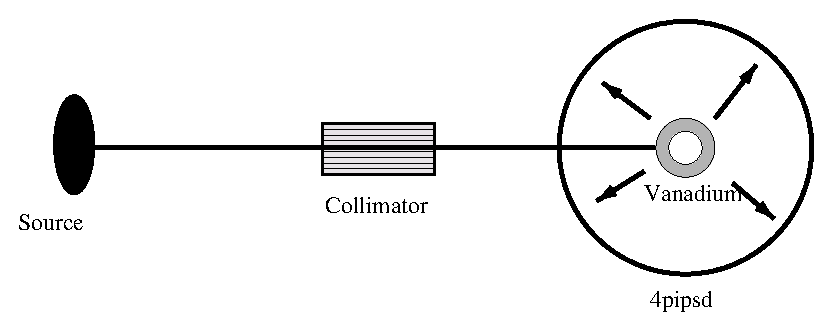
\includegraphics[width=0.9\textwidth]{figures/vanadium.eps}
  \end{center}
\caption{A sketch of the test instrument for the component
V\_sample.}
\label{f:V-instr}
\end{figure}

\subsection{Scattering from the V-sample test instrument}
\label{s:vanadium-result}

In figure \ref{f:V-results}, we present the radial distribution
of the scatting from an evenly illuminated V-sample,
as seen by a spherical PSD.
It is interesting to note that the variation in the
scattering intensity is as large as 10\%. This is an effect
of anisotropic attenuation of the beam in the cylindrical sample.

\begin{figure}
  \begin{center}
    \includegraphics[width=0.6\textwidth]{figures/vanadium-surf-2.eps}
  \end{center}
\caption{Scattering from a V-sample, measured by a spherical
  PSD. The sphere has been transformed onto a plane and the intensity is
  plotted as the third dimension. }
\label{f:V-results}
\end{figure}



\section{The triple axis spectrometer TAS1}
\label{s:TAS1}
With this instrument definition, we have tried to create
a very detailed model of the conventional cold-source
triple-axis spectrometer TAS1 at the now closed neutron source DR3 of
Ris\o\ National Laboratory.
Except for the cold source itself, all components
used have quite realistic properties. Furthermore, the overall
geometry of the instrument has been adapted from
the detailed technical drawings of the real spectrometer.
The TAS 1 simulation was the first detailed work
performed with the \MCS\ package.
For further details see reference~\cite{tas1_report}.

At the spectrometer, the channel from the cold source
to the monochromator is asymmetric, since the first
part of the channel is shared with other instruments.
In the instrument definition, this is represented by
three slits.
For the cold source, we use a flat energy
distribution (component {\bf Source\_flat})
focusing on the third slit.

The real monochromator consist of seven blades, vertically focusing on
the sample. The angle of curvature is constant so that the focusing is
perfect at 5.0 meV (20.0 meV for 2nd order reflections) for a 1$\times$1~cm$^2$
sample. This is modeled directly in the instrument definition using
seven {\bf Monochromator} components. The mosaicity of the pyrolytic
graphite crystals is nominally 30' (FWHM) in both directions.  However, the
simulations indicated that the horisontal mosaicities of both
monochromator and analyser were more likely 45'. This was used for all
mosaicities in the final instrument definition.

The monochromator scattering angle, in effect determining the incoming
neutron energy, is for the real spectrometer fixed by four holes in the
shielding, corresponding to the energies 3.6, 5.0, 7.2, and 13.7~meV for
first order neutrons.  In the instrument definition, we have adapted the
angle corresponding to 5.0~meV in order to test the simulations against
measurements performed on the spectrometer.

The width of the exit channel from the monochromator may
be narrowed down from initially 40~mm
to 20~mm by an insert piece. In the simulations, we have chosen
the 20~mm option and modeled the channel with two slits to match
the experimental set-up.

In the test experiments, we used two standard samples:
An Al$_2$O$_3$ powder sample and a vanadium sample. The instrument
definitions use either of these samples of the correct
size. Both samples are chosen to focus on the opening aperture of
collimator 2 (the one between the sample and the analyser).
Two slits, one before and one after the sample,
are in the instrument definition set to the opening values which
were used in the experiments.

The analyser of the spectrometer is flat and made from
pyrolytic graphite. It is placed between an entry and
an exit channel, the latter leading to a single detector.
All this has been copied into the instrument definition.

On the spectrometer, Soller collimators may be inserted
at three positions: Between monochromator and sample,
between sample and analyser, and between analyser and detector.
In our instrument definition, we have used 30', 28', and 67' collimators
on these three positions, respectively.

An illustration of the TAS1 instrument
is shown in figure~\ref{f:TAS1}.
Test results and data from the real spectrometer are shown
in Appendix~\ref{data:TAS1}.

\begin{figure}
  \begin{center}
    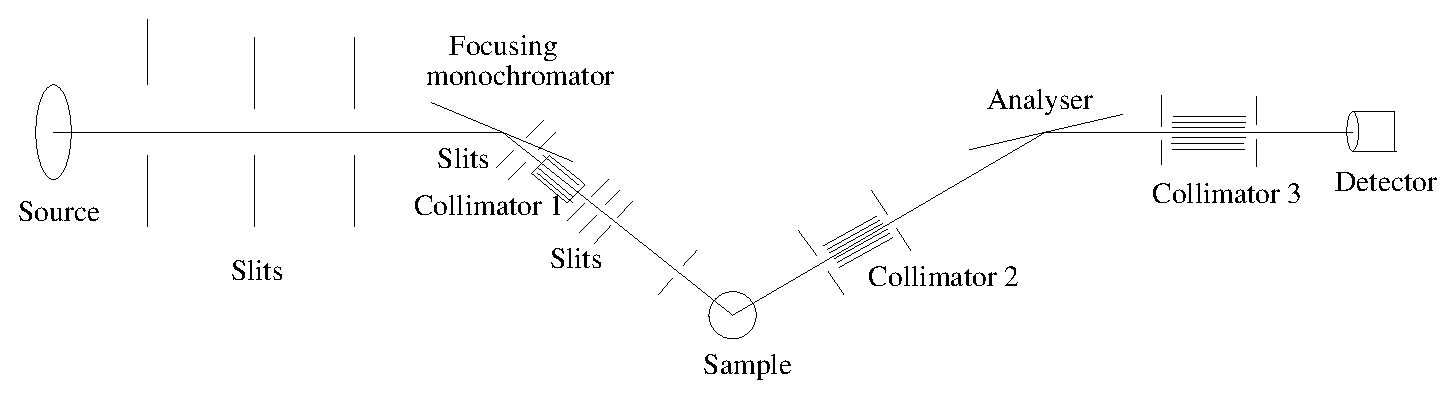
\includegraphics[width=0.9\textwidth]{figures/tas1.eps}
  \end{center}
\caption{A sketch of the TAS1 instrument.}
\label{f:TAS1}
\end{figure}

\subsection{Simulated and measured resolution of TAS1}
\label{data:TAS1}

In order to test the \MCS\ package on a qualitative level,
we have performed a very detailed comparison of a simulation with a
standard experiment from TAS1. The measurement series
constitutes a complete alignment of the spectrometer,
using the direct beam and scattering from V and Al$_2$O$_3$
samples at an incoming energy of 20.0~meV, using the second order
scattering from the monochromator.

In these simulations, we have tried to reproduce
every alignment scan with respect to position and width
of the peaks, whereas we have not tried to compare
absolute intensities. Below, we show a few comparisons
of the simulations and the measurements.

Figure \ref{f:2t_direct} shows a scan of
$2\theta_m$ on the collimated direct beam in two-axis mode.
A \hbox{1 mm} slit is placed on the sample position.
Both the measured width and non-Gaussian peak shape
are well reproduced by the \MCS\ simulations.

\begin{figure}
  \begin{center}
    \includegraphics[width=0.6\textwidth]{figures/tas1-2T.eps}
  \end{center}
\caption{TAS1: Scans of $2\theta_s$ in the direct beam with 1 mm slit on the
  sample position.
"$\times$": measurements, "o": simulations, scaled to the same intensity
Collimations: open-30'-open-open.}
\label{f:2t_direct}
\end{figure}

In contrast, a simulated $2\theta_a$ scan in triple-axis
mode on a V-sample showed a surprising offset from 0 degrees.
However, a simulation with a PSD
on the sample position showed that the beam center was 1.5~mm
off from the center of the sample, and this was important
since the beam was no wider than the sample itself.
A subsequent centering of the beam resulted in a nice
agreement between simulation and measurements.
For a comparison on a slightly different instrument
(analyser-detector collimator inserted),
see Figure~\ref{f:v_2ta_zero}.

%\begin{figure}
%  \begin{center}
%    \includegraphics[width=0.6\textwidth]{figures/vanadium-plot-1.eps}
%  \end{center}
%\caption{First simulated $2\theta_a$ scan on a vanadium sample.
%Collimations: open-30'-28'-open.}
%\label{f:v_2ta_offset}
%\end{figure}

\begin{figure}
  \begin{center}
    \includegraphics[width=0.6\textwidth]{figures/vanadium-plot-2.eps}
  \end{center}
\caption{TAS1: Corrected $2\theta_a$ scan on a V-sample.
Collimations: open-30'-28'-67'.
"$\times$": measurements, "o": simulations.}
\label{f:v_2ta_zero}
\end{figure}

The result of a $2\theta_s$ scan on an Al$_2$O$_3$
powder sample in two-axis mode is shown in Figure \ref{f:al2o3}.
Both for the scan in focusing mode (+ $-$ +)
and for the one in defocusing mode (+ + +) (not shown),
the agreement between simulation and experiment is excellent.

\begin{figure}
  \begin{center}
    \includegraphics[width=0.6\textwidth]{figures/al2o3-focus.eps}
  \end{center}
\caption{TAS1: $2\theta_s$ scans on Al$_2$O$_3$ in two-axis, focusing mode.
Collimations: open-30'-28'-67'.
"$\times$": measurements, "o": simulations.
A constant background is added to the simulated data.}
\label{f:al2o3}
\end{figure}

As a final result, we present a scan of the energy
transfer $E_a = \hbar \omega$ on a V-sample.
The data are shown in Figure \ref{f:v_ea}.

\begin{figure}
  \begin{center}
    \includegraphics[width=0.6\textwidth]{figures/ea-scan.eps}
  \end{center}
\caption{TAS1: Scans of the analyser energy on a V-sample.
Collimations: open-30'-28'-67'.
"$\times$": measurements, "o": simulations.}
\label{f:v_ea}
\end{figure}


\section{The time-of-flight spectrometer PRISMA}
\label{s:PRISMA}

In order to test the time-of-flight aspect of \MCS, we have
in collaboration with Mark Hagen, now at SNS, written a simple
simulation of a time-of-flight instrument loosely based on the ISIS
spectrometer PRISMA. The simulation was used to investigate the effect
of using a RITA-style analyser instead of the normal PRISMA backend.

We have used the simple time-of-flight source {\bf Tof\_source}.
The neutrons pass through a
beam channel and scatter off from a vanadium sample, pass through
a collimator on to the analyser.
The RITA-style analyser consists of seven analyser crystals
that can be rotated independently around a vertical axis. After the
analysers we have placed a PSD and a time-of-flight detector.

To illustrate some of the things that can be done in a simulation as
opposed to a real-life experiment, this example instrument further
discriminates between
the scattering off each individual analyser crystal
when the neutron hits the detector. The
analyser component is modified so that a global variable
\verb+neu_color+ registers which
crystal scatters the neutron ray. The detector component
is then modified to construct seven different time-of-flight histograms,
one for each crystal (see the source code for the instrument
for details). One way to think of this is that
the analyser blades paint a color on each neutron which is then
observed in the detector.
An illustration of the instrument is shown in figure~\ref{f:PRISMA}.
Test results are shown in Appendix~\ref{data:PRISMA}.

\begin{figure}[h]
  \begin{center}
    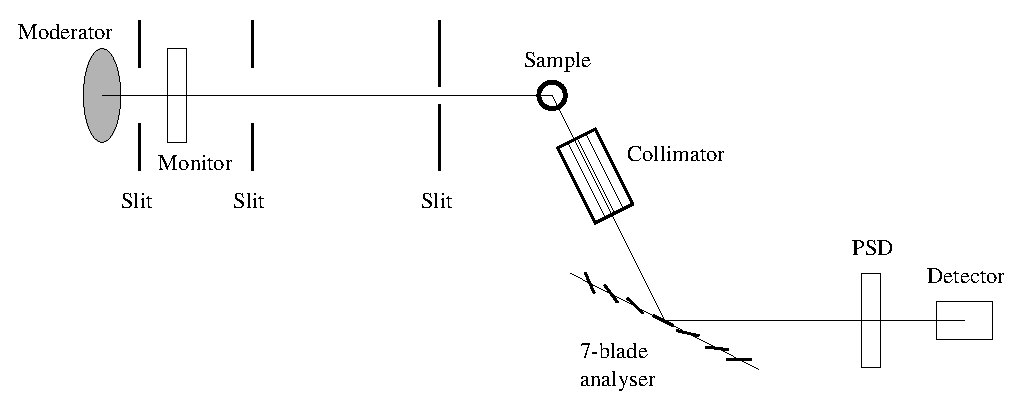
\includegraphics[width=0.9\textwidth]{figures/prisma2.eps}
  \end{center}
\caption{A sketch of the PRISMA instrument.}
\label{f:PRISMA}
\end{figure}

\subsection{Simple spectra from the PRISMA instrument}
\label{data:PRISMA}

A plot from the detector in the PRISMA simulation is shown in Figure
\ref{f:PRISMAdata}. These results were obtained with each analyser blade
rotated one degree relative to the previous one. The separation of the
spectra of the different analyser blades is caused by different energy
of scattered neutrons and different flight path length from source to
detector.  We have not performed any quantitative analysis of the data.

\begin{figure}
  \begin{center}
    \includegraphics[width=0.6\textwidth]{figures/prisma2-a.eps}
  \end{center}
\caption{Test result from PRISMA instrument using ``colored
  neutrons''. Each graph shows the neutrons scattered from one analyser blade.}
\label{f:PRISMAdata}
\end{figure}

%\include{test}   % now in instrum
%\include{future} % now in changes

\appendix
%\documentclass[a4paper]{article}
\usepackage[dvips]{graphicx}
\usepackage{html} 
 \topmargin 0in
\headheight 0in
\headsep 0in
\textheight 7.7in
\textwidth 6.5in
\oddsidemargin 0in
\evensidemargin 0in
\headheight 77pt
\headsep 0.25in
\title{McStas neutron ray-trace tutorial}
\author{Peter Willendrup and Erik Knudsen, DTU Physics}
\begin{document}
\maketitle
{\noindent \small {\bf Postal adress:}\\
DTU Fysik\\Fysikvej 307\\DK-2800
  Kongens Lyngby, Denmark\\\ \\{\bf
    email:}\\\htmladdnormallink{pkwi@fysik.dtu.dk}{mailto:pkwi@fysik.dtu.dk},\htmladdnormallink{erkn@fysik.dtu.dk}{mailto:erkn@fysik.dtu.dk}}
\abstract \noindent This document is a tutorial about McStas and
neutron scattering for beginners.\\\ 
\\The text below is also included as a chapter in the McStas manual
\section{Introduction}
This tutorial has been written to help out novel users of McStas and neutron
scattering instruments. McStas is a software package for simulating
neutron scattering experiments using a Monte Carlo ray-tracing technique. This paper 
aims at helping the user to gain insight into basic neutron scattering 
as well as neutron raytracing using the McStas software package
\cite{McStas0},\cite{Manual},\cite{Websites}.
\subsection{Prerequisites}
Needed knowledge and equipment to work through the tutorial is
\begin{itemize}
\item{Undergraduate knowledge of mathematics and physics.}
\item{A computer with McStas installed (refer to the McStas
    \htmladdnormallink{homepage}{http://mcstas.risoe.dk}
    \cite{Websites} for details) or a bootable McStas Ubuntu live DVD
    (installation to harddisk possible, but not required).}
\item{This tutorial.}
\end{itemize}
\subsection{Goals and tasks}
The goals and tasks of this tutorial are
\begin{itemize}
\item{To teach you about the most basic neutron scattering.}
\item{To let you understand some of the typical components in a
    neutron scattering instrument.}
\item{To teach you basic usage of the McStas neutron simulation
    package.}
\item{To let you create your first McStas instruments, a two axis diffractometer and a triple axis spectrometer.}
\item{To teach you how to modify your instrument for a specific task.}
\item{To help you learn to debug instruments.}
\item{To help you aquire and analyze data from McStas simulations.}
\end{itemize}
\section{Basic neutron scattering}
You may recall the Bragg law from your high school physics
\[n\lambda=2d\sin(\theta),\]
giving the scattering condition for 
a wave of wavelength $\lambda$ against a series of
lattice planes with lattice spacing $d$, rotated the angle $\theta$
off the lattice plane normal. $n$ is an integer giving the spectral
order of the scattered wave. In neutron science one often refers to
the \emph{scattering vector}, $\vec{\kappa}$ of a given reflection, where
\[\kappa=|\vec{\kappa}|=n\frac{2\pi}{d}.\]
This gives us the scattering vector formulation of the Bragg law
\[\kappa=2k\sin(\theta),\]
where $k=\frac{2\pi}{\lambda}$.
%such that
%\[n\lambda=4\pi \kappa^{-1}\sin(\theta)\]
The Bragg law / scattering condition is illustrated in Figure \ref{bragg.eps}.
\begin{figure}[htb!]
\begin{center}
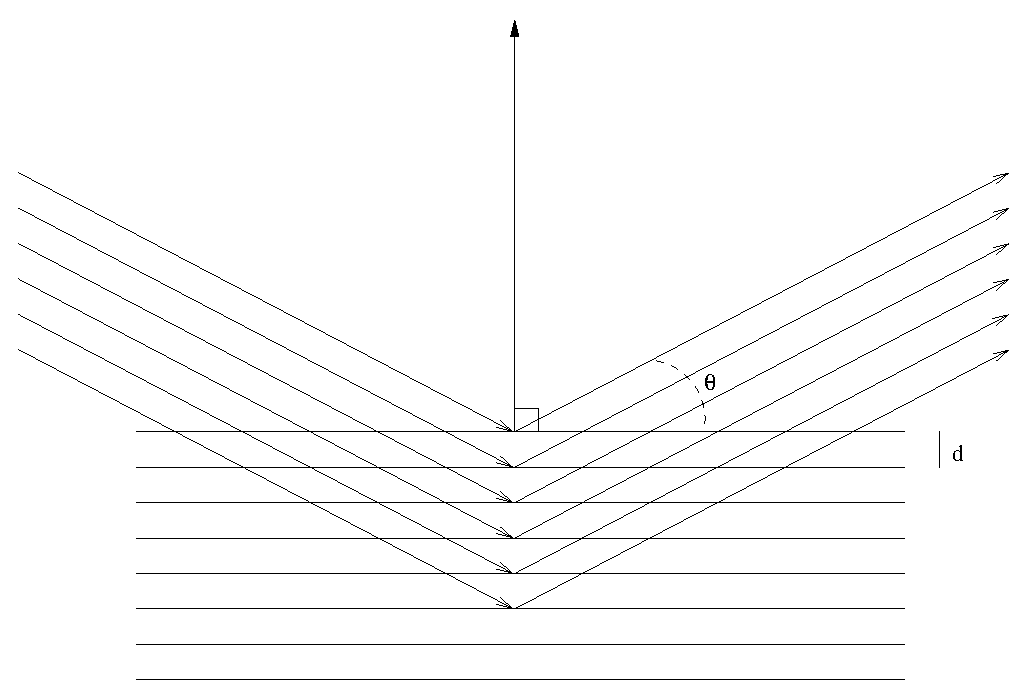
\includegraphics[width=9cm]{pics/bragg.eps}
\end{center}
\caption{Illustration of the Bragg Law.}
\label{bragg.eps}
\end{figure}
Most of the neutron processes we will study in this paper are elastic,
meaning that the wavelength of the neutron is unaltered by the process.
\section{Basic understanding of instrument components}
In the McStas formulation of a neutron scattering instrument, all
objects apart from the neutron ray are referred to as components. This
includes for instance
\begin{itemize}
\item{{\bf Source} The exit of a neutron production facility, where
    neutron rays of certain velocities are emitted into some
    portion of space.}
\item{{\bf Monochromator} (Idealized) crystal that is used to select
    neutrons of a single wavelength\footnote{In reality,
    the monochromator selects a normal distribution of wavelegths
    around $\lambda_0$, and perhaps higher orders as well ($n=2,3,...$
    in Braggs law)} $\lambda_0$ to probe the sample with (monochromator) or to 
    analyze with (analyzer).}
\item{{\bf Sample} An object altering the neutron physical properties
    in some sense, examples used here are:}
  \begin{itemize}
    \item{Vanadium. Scatters incoming neutron rays incoherently.}
    \item{PowderN. Can be thought of as a large number of crystals,
        each scattering neutron rays according to Braggs law, thereby
        producing N concentric Debye Scherrer cones. This sample also
        has the posibility of adding inchoherent, eleastically scattered
        neutron rays.}
    \end{itemize}
\item{{\bf Monitors} Objects \emph{monitoring} or registering neutron ray
    characteristics. In the exercises below are used different types
    of detectors or monitors:}
  \begin{itemize}
    \item{Monitor. Single monitor, detecting the number of neutrons flying
        through a plane. (User defined opening size).}
    \item{PSD\_monitor. Square monitor, detecting the number of
        neutron rays passing through a plane, divided into
        pixels. Square regions of a plane. (User defined resolution 
        and opening size).}
    \item{PSD\_monitor\_4PI. As PSD\_monitor but shaped like a sphere.}
    \item{L\_monitor. Wavelength monitor, measuring the different
        wavelengths of the passing neutron rays. (L is for $\lambda$).}
    \item{Monitor\_nD. General monitor for detecting all sorts of
        physical properties of the neutron ray. In our cases used with
        options:}
      \begin{itemize}
      \item{'single' - as PSD\_monitor but only one small square.}
      \item{'banana' - as PSD\_monitor but shaped like a curved,
          horizontal band.}
      \end{itemize}
    \end{itemize}
  \item{{\bf Collimators}} Devices controling the direction and divergence
   of the neutron ray.
    \begin{itemize}
      \item{Collimator\_linear} A series of parallel absorbing neutron plates
       that limits the beam divergence. 
       Typical values are $6'$ to $120'$.
    \end{itemize}
  \end{itemize}
More information on the McStas components is available by using the
\verb+mcdoc+ program (You may need to set the BROWSER system variable
to your webbrowser of choice):
\begin{itemize}
\item{\verb+mcdoc -s+ , Shows a html list of all the components}
\item{\verb+mcdoc Monitor.comp+ , Shows the documentation for a given component}
\item{\verb+mcdoc -M+ , brings up the McStas manual in PDF format}
\item{\verb+mcdoc -c+ , brings up the McStas component manual in PDF format}
\end{itemize}

\section{Basic McStas}
In short, the core of the McStas system is a precompiler. From a
user-provided instrument description, components are assembled into 
a single piece of \texttt{ansi-c} code. Using a compiler, \emph{e.g.} 
\texttt{gcc}, the c code is compiled into an executable program 
which can be run on your computer. Optionally, the program takes 
input arguments to tune the setup of your instrument/simulation. 
This section will take you through a simple example instrument 
to teach you the basic instrument language of McStas. (Instrument 
filename is vanadium\_example.instr, can be loaded using the
\verb+Neutron Site/Tutorial+ menu item of the \verb+mcgui+, see below).\vspace{1cm}
Please study \emph{carefully} the instructive comments,
marked by \verb+/* ... */+ characters
    
\begin{verbatim}
/* The line below defines the 'name' of our instrument */
/* Here, we have a single input parameter, ROT         */
DEFINE INSTRUMENT vanadium_example(ROT=0)

/* The DECLARE section allows us to declare variables  */
/* in c syntax. Here, coll_div (collimator divergence) */
/* is set to 60 arc minutes...                         */
DECLARE
%{
  double coll_div = 60;
%}

/* Here comes the TRACE section, where the actual      */
/* instrument is defined....                           */
TRACE

/* The Arm() class component defines reference points  */
/* and directions in 3D space. Every component instance*/
/* must have a unique name. Here, arm is used. This    */
/* Arm() component is set to define the origin of our  */
/* global coordinate system (AT (0,0,0) ABSOLUTE)      */
COMPONENT arm = Arm() AT (0,0,0) ABSOLUTE

/* Next, we need some neutrons. Let's place a neutron  */
/* source. Refer to documentation of Source_flat to    */
/* understand the different input parameters.          */
/* The source component is placed RELATIVE to the arm  */
/* component, meaning that modifying the position or   */
/* orientation of the arm will also affect the source  */
/* component (and other components after that one...)  */
COMPONENT source = Source_simple(radius = 0.015, dist = 1,
  xw=0.024, yh=0.015, E0=5, dE=0.2)
 AT (0,0,0) RELATIVE arm

/* Here we have a collimator - placed to improve beam  */
/* divergence. The component is placed at a distance   */
/* RELATIVE to a previous component...                 */
COMPONENT collimator = Collimator_linear(len = 0.2, 
  divergence = coll_div, xwidth = 0.04, yheight=0.06)
  AT (0, 0, 0.4) RELATIVE arm

/* We also need something to 'shoot at' - here a sample*/
/* made from vanadium - an isotrope scatterer. Options */
/* are available to restrict the solid angle in which  */
/* neutrons are emitted (no need to simulate neutrons  */
/* that we know for sure will not reach the rest of    */
/* instrument).                                        */
/* Other options for smart targeting are available -   */
/* refer to component documentation for info.          */
COMPONENT target = V_sample(thickness = 0.004, radius = 0.012, 
  yheight = 0.015, focus_r = 0, pack = 1,
  target_x = 0, target_y = 0, target_z = 1)
  AT (0,0,1) RELATIVE arm

/* Here, a secondary arm - or reference point, placed  */
/* on the sample position. The ROT parameter above     */
/* defines rotation of this arm (and components        */
/* relative to the arm)                                */
COMPONENT arm2 = Arm() 
  AT (0,0,0) RELATIVE target
  ROTATED (0,ROT,0) relative arm

/* For data output, let us place a detector. This      */
/* detector is not very realistic, since it is sphere  */
/* shaped and has a 10 m radius, but has the advantage */
/* that EVERYTHING emitted from the sample will be     */
/* picked up. Notice that this component changes       */
/* orientation with the ROT input parameter of the     */
/* instrument.                                         */
COMPONENT PSD_4pi = PSD_monitor_4PI(radius=10, nx=101, ny=51,
  filename="vanadium.psd")
  AT (0,0,0) RELATIVE arm2
END
\end{verbatim}
Enlightened by the above example, you are probably now ready to learn
a few more important details and tips about McStas.
\begin{itemize}
\item{{\bf Neutron representation:} A neutron 'history' or package is
  an entity representing a large number of neutrons. It has the
  following physical properties:
  \begin{itemize}
    \item{Spatial coordinates, $\vec{x}$ or $x,y,z$.}
    \item{Velocity components, $\vec{v}$ or $v_x,v_y,v_z$.}
    \item{Spin components, $\vec{s}$ or $s_x,s_y,s_z$.}
    \item{Time, $t$.}
    \item{Neutron weight factor, $p$.}
  \end{itemize}
\item{{\bf Neutron histories/Intensities:} McStas simulates neutron
    histories rather than direct neutron counts, \emph{i.e.} when a
    Monte Carlo choice is made in a given component (\emph{e.g.} a random
    number is generated to decide a new direction of the neutron ray), 
    the neutron \emph{weight factor} is adjusted accordingly. As you
    may have guessed already, the weight factor is the 
    average number of of observed neutrons of a given behaviour.
    The transition to direct neutron intensites is made
    by adjusting the initial neutron weight of the source component,
    so that the sum of all simulated weight factors equals the
    absolute intensity of neutrons emitted in one
    second. This means that the intensity of the neutron beam at a
    given position is the initial neutron weight multiplied by the 
    product of all the Monte Carlo weight factors occuring from the
    source to the given position.  When observing McStas output, $I$
    is the intensity, not $N$.}
\item{{\bf 3D space:} The 3D space in which the instrument is defined,
  usually has a single component which is
  placed ABSOLUTEly  in space, \emph{e.g.} at (0,0,0). All other components
  can be placed RELATIVE to this component.}
\item{{\bf Changing coordinate system:} Each component has its own
    local coordinate system. As the neutron travels from one component
    to the other, the local component coordinate system changes. The
    definition is that $z$ is the direction toward the next component,
    and that the $y$ direction is vertical. Our coordinate system is 
    right-handed, making $x$ horisontal and pointing left, looking in 
    the direction of $z$.}
\item{{\bf Component order matters!} It is important to understand
    that McStas is component order dependent. The basic idea is to
    follow the neutron as it travels from one component to the next in
    the instument description. This means that if you place one component
    \emph{geometrically} before another component, but \emph{orderly}
    after the other component, neutrons may never reach your 'first'
    component. This means that some designs can be difficult to
    achieve, though generally a solution can be found.}
\item{{\bf Use Arm()'s!} The Arm() component is very good for defining
  changed orientation of the instrument, \emph{e.g.} for axis turning points
  etc. Placing many Arm()'s will improve future flexibility of your
  instrument.}
\item{{\bf Use PSD\_monitor()'s!} The PSD\_monitor() component is a
    Position Sensitive Detector. This component can
    be used to image the shape of your beam as it travels through the
    instrument. This is very useful for debugging purposes. Other
    monitors, for instance wavelength monitors can also be useful.}}
\end{itemize}
In the McStas manual, available by clicking
\htmladdnormallink{here}{http://mcstas.risoe.dk/documentation/manual/mcstas-1.8-manual.pdf}
if you are using an internet browser to view this document, description
of usage of the different McStas tools is printed. The main McStas
programs are
\begin{itemize}
\item{\emph{mcstas} - Core application.}
\item{\emph{mcgui} - Main graphical user interface.}
\item{\emph{mcdisplay} - Ray trace / debugging application.}
\item{\emph{mcplot} - Data / display application.}
\item{\emph{mcdoc} - Documentation application.}
\end{itemize}
Here are a few hints on using the tools:
\begin{itemize}
\item To start mcgui, execute \verb+mcgui+ in a terminal window
  (\verb+mcgui.pl+ on Windows).
\item To handle instrument files (opening, editing, compiling), use \verb+File+ menu of \verb+mcgui+.
\item To simulate and plot data, use the \verb+Simulation+ menu of \verb+mcgui+.
\item To use the distributed example McStas instruments, use the \verb+Neutron Site+ menu of \verb+mcgui+.
\item For further help on usage, use the items of the \verb+mcgui+
  menu of \verb+Help+ menu or read the chapter \emph{Running McStas}
  of the McStas manual \cite{Manual}.
\end{itemize}
\section{Exercises}
Throughout the rest of this paper, you will have to do the work!
Through a series of small exercises, you will set up and use two simple
neutron scattering instruments: a diffractometer and a triple axis spectrometer. To get an idea of what your final
instrument might look like, see the sample instrument portrayed in Figure \ref{instr.eps}.

In subsection \ref{subsection:examplefile} is shown what the final exercise instrument file might look like. It is advisable to only use this file when stuck as learning by doing (yourself) is preferable to copying.
\begin{figure}[htb!]
\begin{center}
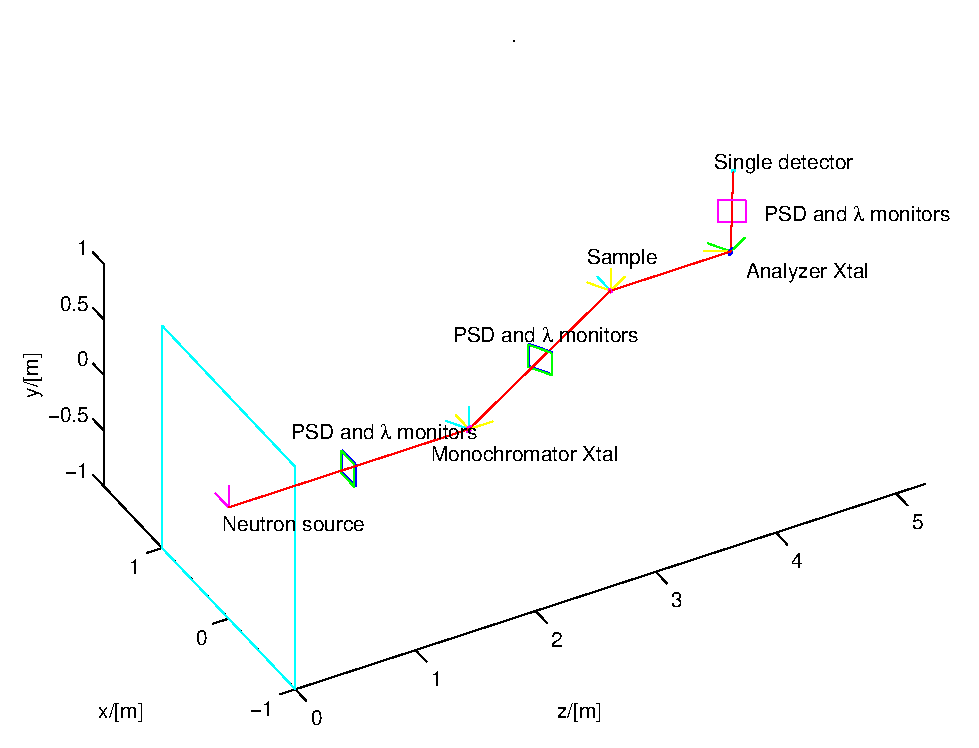
\includegraphics[width=1\linewidth]{pics/instr.eps}
\end{center}
\caption{Illustration of a triple axis diffractometer.}
\label{instr.eps}
\end{figure}
\subsection{Exercise: Source and PSD}
\begin{enumerate}
\item{Start the GUI (Graphical User Interface) by writing the command \verb+mcgui+ in a terminal. To open a terminal in Ubuntu, go to Applications $\rightarrow$ Accessories $\rightarrow$ Terminal or press Ctrl+Alt+t.}
\item{Click the Edit/New button on the GUI.}
\item{Insert a template instrument through the menu Insert $\rightarrow$ Instrument template or by pressing Alt+i twice. Set up an instrument, consisting only of an arm (keep the arm 'Progress\_bar' that is already in the file), a source (Source\_Maxwell\_3) and two monitors (a PSD\_monitor and an L\_monitor). Insert the source at (0,0,0) relative to the origin and the monitors at (0,0,1) relative to the origin. As you input each component you should read the their documentation to find the needed input parameters. The component library can be accessed by clicking the Help (McDoc) button on McGui and choosing 'Component library index'. This will open up an webpage with a list of all the components.

For the source we will help you out. Try
\begin{verbatim}
COMPONENT source = Source_Maxwell_3(
    size = 0.1, l_low = 0.1, l_high = 10, dist = 10, xw = 0.01,
    yh = 0.01, T1 = 300, T2=300, T3=300, I1=1e14, I2=0, I3=0)
AT (0, 0, 0) RELATIVE Origin
\end{verbatim}
Read the Source\_Maxwell\_3 documents using McDoc to understand the suggested parameters.}
\item{When the file is saved for the first time, McGui is automatically given the name of the instrument file. Run a simulation by pressing the Run button in McGui. After compiling the instrument file, McGui will open a window with questions on the simulation such as neutron count, \emph{i.e.} how many times a neutron ray is simulated. For now, simply press the Start button. The instrument simulation will run and its output will be given in the McGui window. When the simulation finishes, plot the results by pressing the Plot button. You should now have two plots, one from the PSD monitor and one from the wavelength monitor. If either or both of the monitors have detected no neutrons, start looking for mistakes in your instrument file.}
\item{Narrow down the interval of wavelengths emitted from the source to \emph{e.g.} l\_low=0.999 and l\_high=1.001. Rerun your simulation to check the effect. Reset the wavelength interval to [0.1 10] \AA.}
\item{Estimate the solid angle covered by your PSD. Try to understand the neutron intensity as illustrated by the plot of the registered events in the PSD in the two previous runs. Try running the simulation with half or double the number of neutron rays. Try also to vary the source focus area and to understand what you observe.}
\end{enumerate}
\subsection{Exercise: Insert a monochromator}
\begin{enumerate}
\item{Keeping your current components, insert a Monochromator\_flat component (use the component library index to get the needed parameters) and a new set of PSD and L\_monitor after the monochromator. Two new arms should be inserted to define the rotation point at the monochromator. One is used to rotate the monochromator, while the other rotates the instrument components that follow. 

Insert the two new arms at (0,0,2) relative to the origin and the monochromator at (0,0,0) relative to the monochromator arm. Also, add two new input parameters of your instrument, which we will call OMM (Omega Monochromator) and TTM (Two Theta Monochromator). These will define the angles of rotation at the monochromator as portrayed in Figure \ref{mono.eps}. 
\begin{figure}[htb!]
\begin{center}
\includegraphics[width=8cm]{pics/mono.eps}
\end{center}
\caption{Illustration of the monochromator orientation.}
\label{mono.eps}
\end{figure}}
\item{Given $\lambda$ = 4\AA, and knowing that for the monochromator $\kappa=1.8734$ \AA$^{-1}$ (Pyrolytic Graphite), use Bragg's law to determine the correct Bragg angle (\emph{i.e.} OMM/TTM) of the monochromator for the $n=1$ reflection. Add the OMM and TTM input parameters to the DEFINE line at the beginning of the instrument file and give them the values you just calculated. Rotate the two arm components by OMM and TTM.}
\item{Do a scan of OMM a couple of angles around the determined Bragg value to verify the finding, while keeping TTM fixed. This is done by replacing the fixed value of OMM in the Run Simulation window with two numbers separated by a comma, \emph{e.g.} 20,25. These numbers represent the minimum and maximum values of OMM. A number of steps must also be given and this is done by changing the \# steps value from 1 to \emph{e.g.} 10. Check the position of the peak on the PSD and the wavelength on the L\_monitor. }
\item{What should $\kappa$ be set to to get the $n=2$ reflection at exactly OMM$=45^\circ$ (TTM$=90^\circ$)? Adjust $\kappa$ for the monochromator and verify the calculation by a scan. Check the wavelength by plotting the scan.}
\item{Determine the Bragg angle for the $n=1$ reflection in this setting of $\kappa$ and verify it by scanning OMM. Set OMM to this value. Perform the simulation and check the wavelength distribution. Comment.}
\item{Before you go on, change the minimum and maximum wavelengths of the source to a suitably narrow interval around 4\AA. There is no need to produce neutron rays that will not be scattered at the monochromator.}
\end{enumerate}
\subsection{Exercise: Insert a sample}
\begin{enumerate}
\item{Now, insert a \verb+V_sample()+ component after the last PSD\_monitor and L\_monitor and a Beamstop component 1.5 m after the sample. The \verb+V_sample()+ component simulates a Vanadium sample. Such a sample scatters incoherently, \emph{i.e.} in all directions. At the same position as the sample, insert a PSD\_monitor\_4PI component of radius 1.0 m. Read the documentation for details on input parameters. Run a simulation. Notice the number of hits.}
\end{enumerate}
\subsection{Exercise: Insert a sample with two powder lines}
\begin{enumerate}
\item{Next, let us insert something more interesting. Remove the V\_sample and  PSD\_monitor\_4PI and insert a PowderN component with the following parameters:
    \begin{verbatim}
COMPONENT sample = PowderN(radius=0.01,h=0.01, d_phi0=0.1, pack=0.5, 
   DW=0.9, frac=0.5, reflections="mylist.dat",
   Vc=3.86*3.86*11.82, sigma_abs=0, sigma_inc=2, barns=1)
  AT (0, 0, 0) RELATIVE \<name of arm at the sample position\>
\end{verbatim}
You should also create a list of reflections and save it as \texttt{mylist.dat}. The list should have the following contents:
\begin{verbatim}
# column_j 3 multiplicity 'j'
# column_q 1  Scattering vector modulus [Angs^-1]
# column_F2 2 Scattering factor |F^2| in [barns]
1 10 8
1.3 10 4
\end{verbatim}
}
\item{Insert a banana shaped detector:
\begin{verbatim}
COMPONENT BananaDetector = Monitor_nD(
   xwidth=2, yheight = 0.09, 
   options="banana, theta limits [-55 -35] bins=360, file =detector.dat")
  AT (0,0,0) RELATIVE sample
\end{verbatim}
and make sure that the previously inserted beamstop is after the banana detector in the component list. Test that neutrons reach the detector by running a simulation. 

Afterwards, choose trace instead of simulate in the Run simulation window and see the instrument, you have created. To see only the trace of the neutrons, which hit the detector, select the detector component in the list given in the Inspect component box. Also, insert the following after the sample component:
\begin{verbatim}
EXTEND %{ 
if (!SCATTERED) ABSORB;
%}
\end{verbatim}
This will insert a command in c-language into the compiled instrument file. The command says that if the simulated neutron does not scatter at the sample, it is absorbed. This removes the direct beam and should be used with caution.}
\end{enumerate}
\subsection{Exercise: Insert a real sample}
\begin{enumerate}
\item{Instead of \texttt{mylist.dat} use \texttt{Na2Ca3Al2F14.laz}. Change the limits of the banana detector to [-10 -130] and change the sample component to read:
\begin{verbatim}
COMPONENT sample = PowderN(
    reflections = "Na2Ca3Al2F14.laz", d_phi = 0.1, radius = 0.004,
    h = 0.03, DW = 0.9, barns = 1, pack = 0.7, frac = 0, tfrac=0)
  AT (0, 0, 2) RELATIVE arm2
\end{verbatim}

Make a simulation to check that a nice powder pattern is observed. If it is time for a coffee break, close the plot from the quick run and instead do a long simulation, \emph{e.g.} 20 million neutron rays, and have coffee.}
\end{enumerate}
\subsection{Exercise: Insert an analyzer}
\begin{enumerate}
\item{Comment out the banana detector and beamstop with /* and */ before and after the components, respectively. Copy the banana detector, but make it to a single detector by changing the options for the Monitor\_nD component to ``single''.}

\item{Add an arm at the sample and an angle to rotate the part of the instrument located after the sample, \emph{e.g.} TT (Two $\Theta$) and decide a more relevant size of the now rectangular detector. Look at your results from the last simulation to determine an approximate scan range for the TT angle, \emph{e.g.} -66.5,-67.5, which will make a scan around the peak at $2\theta=66.94^{\circ}$. Scan TT across one or more powder lines.}

\item{Between sample and detector, set up an analyser crystal by copying and modifying your monochromator component. Add new arms and angles: OMA and TTA; A is for Analyzer. Adjust the analyser to Bragg condition for the chosen wavelength. Re-scan TT and notice the difference to the scan performed in the previous task. Try also scanning around -TT and notice the difference to the other scan. Can you explain the difference?}
\end{enumerate}
\subsection{Example instrument file}\label{subsection:examplefile}
\begin{verbatim}
/*******************************************************************************
*         McStas instrument definition URL=http://www.mcstas.org
*
* Instrument: test (rename also the example and DEFINE lines below)
*
* %Identification
* Written by: Your name (email)
* Date: Current Date
* Origin: Your institution
* Release: McStas CVS-080208
* Version: 0.2
* %INSTRUMENT_SITE: Institution_name_as_a_single word
*
* Instrument short description
*
* %Description
* Instrument longer description (type, elements, usage...)
*
* Example: mcrun test.instr <parameters=values>
*
* %Parameters
* Par1: [unit] Parameter1 description
*
* %Link
* A reference/HTML link for more information
*
* %End
*******************************************************************************/

/* Change name of instrument and input parameters with default values */
DEFINE INSTRUMENT test(OMM=36.607, TTM=73.214, TT=-66.94, OMA=36.607, TTA=73.214)

/* The DECLARE section allows us to declare variables or  small      */
/* functions in C syntax. These may be used in the whole instrument. */
DECLARE
%{
%}

/* The INITIALIZE section is executed when the simulation starts     */
/* (C code). You may use them as component parameter values.         */
INITIALIZE
%{
%}

/* Here comes the TRACE section, where the actual      */
/* instrument is defined as a sequence of components.  */
TRACE

/* The Arm() class component defines reference points and orientations  */
/* in 3D space. Every component instance must have a unique name. Here, */
/* Origin is used. This Arm() component is set to define the origin of  */
/* our global coordinate system (AT (0,0,0) ABSOLUTE). It may be used   */
/* for further RELATIVE reference, Other useful keywords are : ROTATED  */
/* EXTEND GROUP PREVIOUS. Also think about adding a neutron source !    */
/* Progress_bar is an Arm displaying simulation progress.               */
COMPONENT Origin = Progress_bar()
  AT (0,0,0) ABSOLUTE

COMPONENT Source_Maxwell_3 = Source_Maxwell_3(
    size = 0.05, l_low = 3.9, l_high = 4.1, dist = 10, xw = 0.01,
    yh = 0.01, T1 = 150.42, T2 = 38.74, T3 = 14.84, I1 = 3.67E11, I2 = 3.64E11,
    I3 = 0.95E11)
  AT (0, 0, 0) RELATIVE Origin

COMPONENT L_monitor = L_monitor(
    filename = "test2.psd", xmin = -0.1, xmax = 0.1, ymin = -0.1,
    ymax = 0.1, Lmin = 2.1, Lmax = 6)
  AT (0, 0, 1) RELATIVE Origin

COMPONENT PSD_monitor = PSD_monitor(
    nx = 90, ny = 90, filename = "test.psd", xmin = -0.1,
    xmax = 0.1, ymin = -0.1, ymax = 0.1)
  AT (0, 0, 1) RELATIVE Origin

COMPONENT arm1 = Arm()
  AT (0, 0, 2) RELATIVE Origin
  ROTATED (0, OMM, 0) RELATIVE Origin

SPLIT 10 COMPONENT Monochromator_flat = Monochromator_flat(
    zmin = -0.1, zmax = 0.1, ymin = -0.1, ymax = 0.1,
    mosaich = 30, mosaicv = 30)
  AT (0, 0, 0) RELATIVE arm1
EXTEND %{ 
if (!SCATTERED) ABSORB;
%}

COMPONENT arm2 = Arm()
  AT (0, 0, 2) RELATIVE Origin
  ROTATED (0, TTM, 0) RELATIVE Origin

COMPONENT L_monitor2 = L_monitor(
    filename = "test3.psd", xmin = -0.1, xmax = 0.1, ymin = -0.1,
    ymax = 0.1, Lmin = 2.1, Lmax = 6)
  AT (0, 0, 1) RELATIVE arm2

COMPONENT PSD_monitor2 = PSD_monitor(
    nx = 90, ny = 90, filename = "test4.psd", xmin = -0.1,
    xmax = 0.1, ymin = -0.1, ymax = 0.1)
  AT (0, 0, 1.01) RELATIVE arm2

SPLIT 10 
COMPONENT sample = PowderN(
    reflections = "Na2Ca3Al2F14.laz", d_phi = 0.1, radius = 0.004,
    h = 0.03, DW = 0.9, barns = 1, pack = 0.7, frac = 0, tfrac=0)
  AT (0, 0, 2) RELATIVE arm2

/*COMPONENT sample = PowderN(
    reflections = "mylist.dat", d_phi = 0.1, radius = 0.01,
    Vc = 3.86*3.86*11.82, sigma_abs = 0, sigma_inc = 2, h = 0.01,
    DW = 0.9, barns = 1, pack = 0.5, frac = 0.5)
  AT (0, 0, 2) RELATIVE arm2*/
EXTEND %{ 
if (!SCATTERED) ABSORB;
%}

COMPONENT arm3 = Arm()
  AT (0, 0, 0) RELATIVE sample
  ROTATED (0, TT, 0) RELATIVE sample

/*COMPONENT BananaDetector = Monitor_nD(
    xwidth = 2, yheight=0.09, 
    options="banana, theta limits [-10 -130] bins=360, file =detector.dat")
  AT (0, 0, 0) RELATIVE sample

COMPONENT STOP2 = Beamstop(radius=0.3)
AT (0,0,3.5) RELATIVE arm2*/

COMPONENT PSD_monitor3 = PSD_monitor(
    nx = 90, ny = 90, filename = "test5.psd", xmin = -0.132,
    xmax = 0.132, ymin = -0.02, ymax = 0.02)
  AT (0, 0, 0.5) RELATIVE arm3

COMPONENT arm4 = Arm()
  AT (0, 0, 1) RELATIVE arm3
  ROTATED (0, OMA, 0) RELATIVE arm3

SPLIT 10 COMPONENT AnalyzerCrystal = Monochromator_flat(
    zmin = -0.1, zmax = 0.1, ymin = -0.1, ymax = 0.1,
    mosaich = 30, mosaicv = 30)
  AT (0, 0, 0) RELATIVE arm4

COMPONENT arm5 = Arm()
  AT (0, 0, 0) RELATIVE AnalyzerCrystal
  ROTATED (0, TTA, 0) RELATIVE arm3

COMPONENT Analyzer = Monitor_nD(
    xwidth = 0.01, yheight=0.1, 
    options="single, file = analyzer.dat")
  AT (0, 0, 1) RELATIVE arm5



/* This section is executed when the simulation ends (C code). Other    */
/* optional sections are : SAVE                                         */
FINALLY
%{
%}
/* The END token marks the instrument definition end */
END
\end{verbatim}
\section{Suffix}
Well done, you have come to the end of the McStas tutorial. Hopefully,
most of the goals of the tutorials have been fulfilled. Otherwise,
feel free to contact the
\htmladdnormallink{authors}{mailto:peter.willendrup@risoe.dk,kim.lefmann@risoe.dk}
of this paper or the \htmladdnormallink{McStas users
  mailinglist}{mailto:mcstas-users@mcstas.org} for further help.

\begin{thebibliography}{10}
\bibitem{McStas0}
K. Lefmann and K. Nielsen: \emph{McStas, a general software package
  for neutron ray-tracing simulations}, Neutron News, {\bf 10} pp. 20-23, 1999

\bibitem{Manual}
P. Willendrup, E. Farhi K. Lefmann et. al.: \emph{User and Programmers
  Guide to the Neutron Ray-Tracing Package McStas, Version 1.11}, Ris\o\
National Laboratory, Roskilde, Denmark, January 2007\\
\bibitem{Component Manual}
P. Willendrup, E. Farhi K. Lefmann et. al.: \emph{Component Manual for
 the Neutron Ray-Tracing Package McStas, Version 1.11}, Ris\o\
National Laboratory, Roskilde, Denmark, January 2007\\

\bibitem{Websites}
McStas homepage: \url{http://www.mcstas.org}\\
\end{thebibliography}



\end{document}
%% Loads of preamble stripped off - now located in mcstas.tex

%\newpage
\chapter{Polarization in McStas}
\label{c:polarization}
\begin{center}
\Large{P. Christiansen (Ris{\o})\\\today}
\end{center}

\section{Introduction}

In the current release of McStas there are components with polarization
capabilities. At the moment all such components should be understood as under
development as the amount of testing and debugging of these components is
small, and there are known problems.

Here, we shall report on what have been done so far.

We first describe the polarization vector and how it is related to the neutron
wave-function (section~\ref{sec:pol}) and then the physics of simple
components that we need in McStas is reviewed (section~\ref{sec:scat}). In the
last two sections the actual McStas polarization components are first
described (section~\ref{sec:new}) and a list of test instruments in McStas is
given (section~\ref{sec:test}).

We rely heavily on the books~\cite{lovesey84,gavin} for the physics where
the detailed calculations can be found.

The notation used here (and in~\cite{gavin}) is $P$ (scalar), $\PB$
(vector), $\tP$ (unit-vector), $\sigmaH$ (operator), and $\sigmao$
(vector of operators).

\section{The Polarization Vector}
\label{sec:pol}

The spin of the neutron is represented by an operator $\so$ for which only a
single component can be measured at one time. Each single measurement will
give a value $\pm 1/2$, but if we could make a large number of measurements on
the same neutron state, in each of the three axis directions, and then make
the average we get $\langle \so \rangle$. The polarization vector, $\PB$, is
then defined as:
\begin{equation}
  \label{eq:pol_single}
  \PB = \frac{\langle \so \rangle}{s},
\end{equation}
so that $-1 \leq |\PB| \leq +1$

For a neutron beam which contains $N$ neutrons, each with a
polarization $\PB_i$, the beam polarization is defined as:
\begin{equation}
  \label{eq:pol_beam}
  \PB = \frac{\sum_i \PB_i}{N}.
\end{equation}

If we have one common quantization direction (e.g. a magnetic field
direction) each neutron will either be spin up, $\uparrow$, or spin down,
$\downarrow$, and the polarization can be expressed as:

\begin{equation}
  \label{eq:pol}
  P = \frac{\nup-\nd}{\nup+\nd},
\end{equation}

where $\nu$ ($\nd$) is the number of neutrons with spin up
(down).

For a given neutron the probability of the neutron being spin up, $\Pu$, is:

\begin{equation}
  \label{eq:prob_spinup}
  \Pu = \frac{\nup}{\nup+\nd} = \frac{\nup + (\nd-\nd)/2}{\nup+\nd}
  = \frac{1+P}{2},
\end{equation}

and $\Pd = 1-\Pu = (1-P)/2$.

The expectation value of the 'spin' operator, $\sigmao$, which can be
expressed by the Pauli matrices, is the polarization vector $\PB$, $\PB =
\langle \sigmao \rangle \equiv \langle \chi | \sigmao | \chi \rangle$.  The
most general form of the spin wave-function $\chi$ for a neutron (spin 1/2)
is:

\begin{equation}
  \label{eq:neutron_wave}
  \chi = a\chi_\uparrow + b\chi_\downarrow,
\end{equation}

where $\chi_\uparrow$ and $\chi_\downarrow$ are eigenfunction of
$\hat{\sigma}^z$, and the complex coefficients $a$ and $b$ satisfy
$|a|^2 + |b|^2 = 1$.

By calculation we find:
\begin{eqnarray}
P_x & = & \langle \chi | \sigmaH_x | \chi \rangle
= 2 \text{Re}(a^\ast b) \\
P_y & = & \langle \chi | \sigmaH_y | \chi \rangle
= 2 \text{Im}(a^\ast b) \\
P_z & = & \langle \chi | \sigmaH_z | \chi \rangle
= |a|^2-|b|^2
\end{eqnarray}

This shows the relation of the polarization vector to the neutron wave
function.

The neutron magnetic moment operator can be expressed in terms of $\sigmao$,
as:
\begin{equation}
  \label{eq:magnetic}
  \muno = \mu_n \sigmao,
\end{equation}
which, as shown above, is related to the polarization vector.  \\

In our simulation we represent the polarization by the vector $\SB = (s_x,
s_y, s_z)$ which is propagated through the different components so it has the
correct relative orientation in each component. The probability for the spin
to be parallel a given direction $\mathbf{n}$ is then:

 \begin{equation}
   \label{eq:probmcstas}
   P(\uparrow|\nB) = \frac{1+\nB \cdot \SB}{2}.
 \end{equation}

This equation (from~\cite{pol_seeger}) is easy to understand. The
average spin along $\nB$ is $\nB \cdot \SB$ and the probability then
follows from Eq.~\ref{eq:prob_spinup}.

For an unpolarized beam, $\mathbf{S} = \mathbf{0}$ and all directions
are equally probable (50~\%).

Note that in our approach we do not decide if the neutron is up or down after
a given component, but instead keep track of as much information for as long
as possible.

In the following we will use $\PB$ to denote the polarization
vector. The most important variables used are:

\begin{tabular}{ll}

  $\Q$  & Scattering vector. \\
  $\PB$  & Polarization before a component (ingoing). \\
  $\PB_\perp$  & Polarization perpendicular to scattering vector,
  $\PB_\perp = \tQ \times (\PB \times \tQ$). \\
  $\PB'$ & Polarization after a component (outgoing). \\
  $\tN$ & Unit vector in direction of atomic spin ($\tN \cdot \tilde{\BB} = -1$ for a ferromagnet). \\
  $\FN$ & Unit cell nuclear structure factor. \\
  $\FM$ & Unit cell magnetic structure factor. \\
\end{tabular}
\\

The unit cell nuclear structure factor is defined as:

\begin{equation}
  \FN = \sum_\dB
  \exp(i\Q \cdot \dB)\overline{b}_d,
\end{equation}

where the $\dB$ is the position of the d'th atom within the unit cell,
and $\overline{b}_d$ is the average of $b_d$. In the simple case of a
single atom Bravais crystal one finds $\FN = \overline{b}$.

The unit cell magnetic structure factor is useful when the atoms in
the crystal only have spin orbital angular momentum, and simple when
the magnet is saturated (all spins are parallel or anti-parallel to
\emph{one} direction, $\sigma_d=\pm1$). It is then given as:

\begin{equation}
  \FM =
  \gamma_n r_0 \sum_\dB \exp(i\Q \cdot \dB)\frac{1}{2}g_d F_d(\Q)\langle
  \hat{S}_d\rangle \sigma_d,
\end{equation}

where $r_0=\frac{\mu_0}{4\pi}\frac{e^2}{m_e} = 2.818 \times 10^{-15}$m, $g=2$ is the
Land{\'e} splitting factor, and $F_d(\Q)$ is the magnetic form factor, which
is the Fourier transform of the magnetization density (normalized so that
$F_d(0) = 1$), and $\langle \hat{S}_d\rangle$ is the thermal average of the
ordered atomic spin.

In the following the Debye-Weller factor ($\exp(-W_d)$) have been ignored in
all cross sections.

\subsection{Example: Magnetic fields}

The magnetic moment operator of the neutron is $\muno = \gamma_n \so$, where
$\gamma_n = 2 \mu_n = -3.826$ is the gyromagnetic ratio (spin and magnetic
moment is anti-parallel as for an electron)~\footnote{Note that if we had used
S (with values $S=\pm 1$) to define $\gamma_n$ we would get $\gamma_n =
-1.913$ which is also commonly used.}

A magnetic field, $\BB$, will exert a torque, $\tauB = d\sB/dt = (1/\gamma_n)d\muB/dt$, on the neutron magnetic moment:

\begin{equation}
  \label{eq:torque}
  \frac{1}{\gamma_n} \frac{d\muB}{dt} = \muB \times \BB
\end{equation}

The magnetic moment $\mu$ can be related to the polarization as $\muB
= \gamma_n \PB/2$, and inserting in Eq.~\ref{eq:torque} we find:

\begin{equation}
  \label{eq:pol_magnetic}
  \frac{d\PB}{dt} = \gamma_n \PB \times \BB
\end{equation}

In the simple case where $\BB = (0, 0, B)$, we find the solution
(\cite{gavin} p.~18) :

\begin{eqnarray}
  \nonumber
  P_X(t) & = & \cos(\omega_L t) P_X(0) - \sin(\omega_L t) P_Y(0) \\
  \label{eq:precession}
  P_Y(t) & = & \sin(\omega_L t) P_X(0) + \cos(\omega_L t) P_Y(0) \\
  \nonumber
  P_Z(t) & = & P_Z(0),
\end{eqnarray}

where $\omega_L = -\gamma_n B/\hbar$ is the Larmor frequency.\\

\begin{quote}
  The equations above was checked against the equations in the ``polarimetrie
  neutronique'' notes by Francis Tasset and found to be consistent. There can
  be sign differences between different publications depending on whether they
  use a right-handed (like e.g. McStas) or a left-handed (like e.g. NISP)
  coordinate system.
\end{quote}

\section{Polarized Neutron Scattering}
\label{sec:scat}

First we will give a short introduction to how calculations are done
and then quote some results which are important for implementing the
first McStas components.

All the potentials (nuclear, magnetic, and electric) we will be interested in
can be written on the form:
\begin{equation}
  \label{eq:general_pot}
  \hat{v} = \betao + \alphao \cdot \sigmao
\end{equation}

The first term does not affect the spin, while the second term can
change the spin. Let us just remind here that:

\begin{equation}
  \label{eq:pauli_rules}
  \begin{matrix}
    \sigmaH_x \chiU = \chiD, &
    \sigmaH_y \chiU = i\chiD, &
    \sigmaH_z \chiU = \chiU, \\
    \sigmaH_x \chiD = \chiU, &
    \sigmaH_y \chiD = -i\chiU, &
    \sigmaH_z \chiD = -\chiD.
  \end{matrix}
\end{equation}

So that the interaction proportional to $\sigmaH_x$ and $\sigmaH_y$
results in spin flips, while the interactions with $\sigmaH_z$
conserves the spin.

It turns out to be smart to define a density matrix operator:
\begin{equation}
  \rhoo = \chi \chi^\dagger =
  \left( \begin{matrix}
    |a|^2 & ab^\ast \\
    ba^\ast & |b|^2
  \end{matrix} \right)
  = \frac{1}{2}({\cal I}+\PB \cdot \sigmao),
\end{equation}
where $\chi$ is the neutron wave function (Eq.~\ref{eq:neutron_wave}),
and ${\cal I}$ is the unit matrix.

Using the density matrix the elastic cross section can be written as
(\cite{lovesey84}, Eq.~10.31):
\begin{equation}
  \label{eq:master_sigma}
  \frac{d\sigma}{d\Omega} = \text{Tr} \rhoo \hat{v}^\dagger \hat{v}
  = \sum_{\lambda, \lambda'} p_\lambda \text{Tr} \rhoo
  \langle \lambda | \hat{V}^\dagger(\Q) | \lambda' \rangle
  \langle \lambda' | \hat{V}(\Q) | \lambda \rangle
  \delta(E_\lambda - E_{\lambda'}),
\end{equation}

where $\hat{V}$ is the interaction potential and it is understood that
the trace is to be taken with respect only to the neutron spin
coordinates. The outgoing polarization is given as:
\begin{equation}
  \label{eq:master_pol}
  \PB' \frac{d\sigma}{d\Omega} =
  \text{Tr} \rhoo \hat{v}^\dagger \sigmao \hat{v}
  = \sum_{\lambda, \lambda'} p_\lambda \text{Tr} \rhoo
  \langle \lambda | \hat{V}^\dagger(\Q) | \lambda' \rangle
  \sigmao
  \langle \lambda' | \hat{V}(\Q) | \lambda \rangle
  \delta(E_\lambda - E_{\lambda'})
\end{equation}

Inserting Eq.~\ref{eq:general_pot} in Eq.~\ref{eq:master_sigma} and
Eq.~\ref{eq:master_pol} results in the two master equations for
polarized neutron scattering:

\begin{equation}
  \label{eq:general_sigma}
  \text{Tr} \rhoo \hat{v}^\dagger \hat{v} =
  \alphao^\dagger \cdot \alphao + \betao^\dagger \betao+
  \betao^\dagger (\alphao \cdot \PB) +
  (\alphao^\dagger \cdot \PB) \betao +
  i\PB \cdot (\alphao^\dagger \times \alphao),
\end{equation}

and

\begin{equation}
  \label{eq:general_pol}
  \text{Tr} \rhoo \hat{v}^\dagger \sigmao \hat{v} =
  \betao^\dagger \alphao
  + \alphao^\dagger \betao
  + \betao^\dagger \betao \PB
  + \alphao^\dagger (\alphao \cdot \PB)
  + (\alphao^\dagger \cdot \PB) \alphao
  - \PB (\alphao^\dagger \cdot \alphao)
  - i \alphao^\dagger \times \alphao
  + i \betao^\dagger (\alphao \times \PB)
  + i (\PB \times \alphao^\dagger) \betao.
\end{equation}

Based on these two equations and the interaction potentials all the
results presented in the following are derived in~\cite{lovesey84}.

\subsection{Example: Nuclear scattering}

The nuclear scattering potential for a crystal is:
\begin{equation}
  \label{eq:nuclear_pot}
  \hat{V}_N(\Q) = \sum_{\lB,\dB} \exp(i\Q \cdot \RB_{ld})(A_{ld} +
  \frac{1}{2} B_{ld} \sigmao \cdot \Io_{ld}),
\end{equation}

so that

\begin{eqnarray}
  \label{eq:ab_nuclear}
  \alphao & = &
  \sum_{\lB,\dB} \exp(i\Q \cdot \RB_{ld}) \frac{1}{2} B_{ld} \Io_{ld} \\
  \betao & = &
  \sum_{\lB,\dB} \exp(i\Q \cdot \RB_{ld}) A_{ld},
\end{eqnarray}

where $\Io$ is the nuclear spin operator and the constants $A$ and $B$
are related to the nuclear scattering lengths $b^+$ and $b^-$ as
$A=((I+1)b^++Ib^-)/(2I+1)$ and $B=(b^++b^-)/(2I+1)$.

To calculate the polarization cross section and outgoing polarization
we have to average over the nuclear spin (which we assume is random
oriented), so that terms linear in $\alphao$ (three last terms in
Eq.~\ref{eq:general_sigma}) disappears. The scattering cross section
ends up being (see~\cite{lovesey84} p.~159):

\begin{equation}
  \label{eq:nuclear_sigma}
  \frac{d\sigma}{d\Omega}  =
  \sum_{\lB, \dB, \lB', \dB'} \exp(i \Q \cdot (\RB_{ld}-\RB_{l'd'}))
  (\madsq + \delta_{\lB,\lB'}\delta_{\dB,\dB'}[\sqmad - \madsq
  + \frac{1}{4}\bd])
\end{equation}

where the first term is the coherent cross-section and the second term is the
site-incoherent cross-section. Both terms are independent of $\PB$ as expected
for a system without a preferred internal direction.

The polarization in the final state is:

\begin{equation}
  \label{eq:nuclear_pol}
  \PB' \frac{d\sigma}{d\Omega}  =
  \sum_{\lB, \dB, \lB', \dB'} \exp(i \Q \cdot (\RB_{ld}-\RB_{l'd'}))
  \PB' (\madsq + \delta_{\lB,\lB'}\delta_{\dB,\dB'}[\sqmad - \madsq
  - \frac{1}{12}\bd])
\end{equation}

Comparing Eq.~\ref{eq:nuclear_sigma} and Eq.~\ref{eq:nuclear_pol} we
find that: 1) The nuclear coherent polarization is the same as the
initial polarization. 2) The same is true for the incoherent
scattering due to the random isotope distribution. 3) The nuclear
incoherent scattering due to the random nuclear spin orientations has
polarization $\PB' = -1/3 \PB$ (for a random nuclear spin the
associated Pauli matrix will 2/3 of the time point in the direction of
$\sigmaH_x$ and $\sigmaH_y$ which according to
Eq.~\ref{eq:pauli_rules} flips the spin). \\

For Vanadium, where there is only one isotope and coherent scattering
is negligible, we find $\PB' = -1/3\PB$. There is however one
catch. If the probability for multiple scattering is large one has to
take into account that after two scattering one has: $\PB'(2) =
1/9\PB$, and so forth. The average polarization after a thick vanadium
target is therefore a sum of different contributions.

\subsection{Example: Polarizing Monochromator and Guides}
\label{sub:mono}

\begin{figure}[htbp]
  \begin{center}
    \includegraphics[keepaspectratio,
    width=0.7\columnwidth]{figures/monochromator_pol}
    \caption{Principle and geometry of a polarizing monochromator.}
    \label{fig:mono_princip}
  \end{center}
\end{figure}

In a polarized monochromator and polarizing guides we have a ferromagnetic
crystal in an external magnetic field. The scattering potential is now both
nuclear (no internal direction) and magnetic (internal direction), so in
general the outgoing polarization can be quite complex. However, as
illustrated in Figure~\ref{fig:mono_princip}, the typical setup has many
geometrical constraints: $\tN \cdot \tQ = 0$, $\tN \cdot \PB_\perp = \tN \cdot
\PB$, and $\Q \times (\tN \times \Q) = \tN$, which simplifies the problem.

In~\cite{lovesey84} the calculation for a centrosymmetric ferromagnetic
crystal is done, and inserting the constraints above one finds
(\cite{lovesey84}, Eq.~10.96 and Eq.~10.110):

\begin{eqnarray}
  \label{eq:mono_sigma}
  d\sigma/d\Omega & = & \FN^2 + 2\FN\FM (\PB \cdot \tN) + \FM^2\\
  \label{eq:mono_pol}
  \PB' d\sigma/d\Omega & =
  & \PB [\FN^2 - \FM^2] + \tN [2\FN\FM + 2(\tN \cdot \PB)\FM^2]
\end{eqnarray}

\begin{quote}
  NB! Note that in~\cite{gavin} Eq.~2.2.25 there is a minus in front of the
  second term in Eq.~\ref{eq:mono_sigma}. We have not been able to understand
  this discrepancy, which is probably due to notation. Most other authors
  agree with the minus in front of the second term (e.g. Squires and Francis
  Tasset).
\end{quote}

For a beam which is initially unpolarized we find the outgoing
polarization to be:
\begin{equation}
  \PB' = \frac{\tN 2\FN \FM}{d\sigma/d\Omega}
  = \frac{2\FN\FM}{\FN^2 + \FM^2} \tN,
\end{equation}

so that the beam is fully polarized along $\tN$ if $\FN = \pm \FM$. \\

What we use to characterize the polarizing monochromator in practice
is not $\FN$ and $\FM$, but instead the reflection probabilities $\Ru$
and $\Rd$ (for the reflection of interest).

If we assume that the reflection probabilities are directly proportional to
the cross sections (with proportionality constant $k$), i.e., $\Ru = k
d\sigma/d\Omega(\PB=+\tN)$ and $\Rd = k d\sigma/d\Omega(\PB=-\tN)$ then we can
use Eq.~\ref{eq:mono_sigma} to determine $\FN$ and $\FM$:

\begin{eqnarray}
  \label{eq:mono_up}
  \Ru & = & k (\FN + \FM)^2,\\
  \label{eq:mono_down}
  \Rd & = & k (\FN - \FM)^2.
\end{eqnarray}

The values of $\sqrt{k}\FN$ and $\sqrt{k}\FM$ are then between -1 and +1 and
unit less like the reflection probabilities. In the following we ignore $k$ and
just talk about $\FN$ and $\FM$.

In principle there are four solutions for $\FN$ and $\FM$, so in the code we
currently choose the values where $\FN + \FM = +\sqrt{\Ru}$ and $\FN - \FM =
+\sqrt{\Rd}$ (so that $\FN>0$ and $\FN>\FM$). We then find:

\begin{eqnarray}
  \label{eq:mono_nuc}
  \FN & = & \frac{\sqrt{\Ru} + \sqrt{\Rd}}{2},\\
  \label{eq:mono_mag}
  \FM & = & \frac{\sqrt{\Ru} - \sqrt{\Rd}}{2}.
\end{eqnarray}

When $\FN$ and $\FM$ are determined from these equations,
Eq.~\ref{eq:mono_sigma} and Eq.~\ref{eq:mono_pol} can easily be used to handle
any situation.

This solution is both used for monochromators and guides.

It is not clear that this solution is correct. If we make a simple example
with $\Ru = 1$ and $\Rd = 0.25$ then we could in principle have four
solutions, but let us just quote the two where $\FN$ is positive since the
last two are found by inserting a minus before all the solutions and this does
not change the physics. The two solutions are $\FN = 0.75, \FM=0.25$ and $\FM
= 0.75, \FN=0.25$. All solutions gives the same cross section, but if the
incoming beam is polarized (and only then) the outgoing beam will have two
different polarization values, since $\PB [\FN^2 - \FM^2]$ and $\tN 2(\tN
\cdot \PB)\FM^2$ are different for the two solutions. It seems that one needs
some additional information to choose between the two solutions.

\begin{quote}
  NB! The simplifying geometry shown in Figure~\ref{fig:mono_princip} only
  applies for the sides of the guide wall and not the top and bottom (assuming
  that the magnetizing field is pointing up or down), so there another set of
  equations should really be used.
\end{quote}

The same physics could also be used for a polarizing powder or single crystal
sample if $\FN$ and $\FM$ can be calculated with some other program, but one
would have to use the general form of Eq.~\ref{eq:mono_sigma} and
Eq.~\ref{eq:mono_pol} without the simplifying geometrical constraints for
monochromators and guides.

\section{New McStas Components}
\label{sec:new}

The components written so far can be divided into four groups:
\begin{itemize}
\item \textbf{Polarizers:} Components used to make the beam polarized.
\item \textbf{Monitors:} Unphysical detectors that can measure the polarization
of the neutrons.
\item \textbf{Magnetic fields:} Components used to handle magnetic fields.
\item \textbf{Samples:} Samples that affects the polarization.
\end{itemize}

\subsection{Polarizers}

Some of the most common ways of polarizing a beam have been
implemented.

\begin{itemize}
\item \textbf{Set\_pol:} This unphysical component can be used in two
ways. Either to hard code the polarization to the vector $(px, py, pz)$
or when randomOn!=0 to set the polarization vector to a random vector
on the unit sphere.\\

\item \textbf{Monochromator\_pol:} A monochromator that only does the $n=1$
  reflection. For each neutron it calculates the wavelength which would give
  Bragg reflection, $\lambda_\text{Bragg}$, and it then calculates, based on
  one mosaicity and one d-spread, the reflection probability given the neutrons
  actual $\lambda$.  The reflection probability is a Gaussian in $\Delta
  \lambda = \lambda - \lambda_\text{Bragg}$, with the peak reflectivity and
  polarization calculated as described in section~\ref{sub:mono}.

  \begin{quote}
    NB! Note that this monochromator reflects the neutrons billiard-like. In
    \textbf{Monochromator\_flat} the mosaicity of the reflecting crystal is
    taken into account, but the d-spread is not taken into account. One should
    implement d-spread and mosaicity in a way similar to what is done in
    \textbf{Single crystal}.
  \end{quote}

\item \textbf{Pol\_mirror:} Plane with a reflection probability for up
and down. There are 3 options: always reflect, always transmit, or
random select transmit/reflect.

\begin{quote}
  NB! Note that at the moment the plane only reflects from one side (because
  it uses PROP\_Z0.
\end{quote}

\item \textbf{Pol\_bender:} Curved guide with the possibilities to
  insert multiple slits, and have the end gap parallel to the entrance
  or following the guide angle. It is possible to select different
  coatings (mirror parameters) for each of the four sides.\\

\item \textbf{Pol\_guide\_vmirror:} Straight guide with non-polarizing
  coatings with two polarizing super mirrors sitting in a V shape
  inside. \\
\end{itemize}

Note that for all the polarizing guides it is possible to define analytical
functions or use tables for the up and down reflectivity descriptions.

\subsection{Detectors}

\begin{itemize}
\item \textbf{Pol\_monitor:} One defines a vector $\mathbf{m} = (mx,
  my, mz)$ for the monitor and measures the projection of the spin
  along this vector i.e. $\mathbf{m} \cdot \mathbf{S}$.\\

\item \textbf{PolLambda\_monitor:} Measures the projection of the
  spin along the defined vector $\mathbf{m}$ (see
  \textbf{Pol\_monitor}) as a function of the wavelength $\lambda$.

\item \textbf{MeanPolLambda\_monitor:} Measures the \emph{average}
  projection of the spin along the defined vector $\mathbf{m}$ (see
  \textbf{Pol\_monitor}) as a function of the wavelength $\lambda$.

  \begin{quote}
    NB! currently the error on the mean is shown ($\sigma/\sqrt(N)$), but it
    might make more sense to show the spread ($\sigma$).
  \end{quote}
\end{itemize}

\subsection{Magnetic fields}

Much inspiration for the components and the tests have been found
in~\cite{pol_seeger}.

\begin{itemize}
\item \textbf{Pol\_constBfield:} A rectangular box with a constant magnetic
  field in the y-direction. The x- and z-components of the spin precess with
  the Larmor frequency $\omega_L$. It is possible to define the field in terms
  of a wavelength so that the spin will precess 180 degrees for the given
  wavelength. The component can be rotated to have the field along another
  axis. \\

\item \textbf{Pol\_simpleBfield:} The first attempt at a component for
  handling general magnetic fields. It is a concentric component where you
  define a start and stop component for each field, but this allows other
  components, e.g. monitors, to be put inside the field. The component
  overloads the propagation routines so that numerical spin propagation is
  done for analytical magnetic fields.

  \begin{quote}
    NB! At the moment both components does not really check the boundaries of
    the field on the sides, but merely assumes that the field starts at the
    entrance plane and stops at the exit plane.

    Also, some optimization remains for the numerical component and it would
    be nice to support tabulated magnetic field files. However, the framework
    developed for \textbf{Pol\_simpleBfield} is very general and should
    easily facilitate these changes.
  \end{quote}

\end{itemize}


\subsection{Samples}

\begin{itemize}
\item \textbf{V\_sample:} Modified the sample so that the scattered
  neutron has $\PB' = -1/3\PB$. Note that this component does not
  handle multiple scattering, so this approach is correct. If the
  components handled multiple scattering the polarization should be
  set to $\PB' = (-1/3)^n\PB$, where $n$ is the number of
  scatterings.\\
\end{itemize}


\section{Tests With New Components}
\label{sec:test}

All the test instruments can be found in the McStas examples folder
(go to ``Neutron site/tests'' in mcgui).

There are basically two kind of tests. The first kind of tests shows
that the polarizing component can reproduce the same results as a
similar non-polarizing component:
\begin{itemize}
\item \textit{Test\_Monochromators.instr} : Intercomparison of
  \textbf{Monochromator\_flat} and \textbf{Monochromator\_pol}.
\item \textit{Test\_Pol\_Bender\_Vs\_Guide\_Curved.instr} : Intercomparison of
  \textbf{Guide\_curved} and \textbf{Pol\_bender}.
\end{itemize}

The second type of test illustrates the polarizing capabilities of the
component:
\begin{itemize}
\item \textit{Test\_Magnetic\_Constant.instr} : Constant magnetic field.
\item \textit{Test\_Magnetic\_Majorana.instr} : Linearly decreasing field with
  small transverse component.
\item \textit{Test\_Magnetic\_Rotation.instr} : Rotating magnetic field.
\item \textit{Test\_Magnetic\_Userdefined.instr} : Example of how to make a
  user defined analytic magnetic field that can also depend on time.
\item \textit{Test\_Pol\_Bender.instr} : Illustrates beam polarization with
  the \textbf{Pol\_bender}.
\item \textit{Test\_Pol\_Set.instr} : Tests \textbf{Pol\_set}.
\item \textit{Test\_Pol\_Guide\_Vmirror.instr} : Illustrates beam polarization
  with the \textbf{Pol\_guide\_vmirror}.
\item \textit{Test\_Pol\_Mirror.instr} : Illustrates beam polarization
  with the \textbf{Pol\_mirror}.
\item \textit{Test\_Pol\_TripleAxis.instr} : An example of a triple axis
  spectrometer with polarizing monochromators, a vanadium sample, and a spin
  flipper.
\end{itemize}


\chapter{Random numbers in \MCS}
\label{s:random}
\index{Monte Carlo method}

\section{Transformation of random numbers}
In order to perform the Monte Carlo choices, one needs to be able to
pick a random number from a given distribution. However, most
random number generators only give
uniform distributions over a certain interval.
We thus need to be able to transform between probability distributions,
and we here give a short explanation on how to do this.

Assume that we pick a random number, $x$, from a distribution $\phi(x)$.
We are now interested in the shape of the distribution, $\Psi(y)$, of the
transformed $y=f(x)$, assuming $f(x)$ is monotonous.
All random numbers lying in the interval $[x; x+dx]$
are transformed to lie within the interval $[y; y+f'(x)dx]$, so the
resulting distribution must be $\Psi(y) = \phi(x) / f'(x)$.

If the random number generator selects numbers uniformly in the interval
$[0; 1]$, we have $\phi(x) = 1$ (inside the interval; zero outside), and
we reach
\begin{equation}
\Psi(y) = \frac{1}{f'(x)} = \frac{d}{dy} f^{-1}(y) .
\end{equation}
By indefinite integration we reach
\begin{equation}
\label{e:randtrans}
\int \Psi(y) dy = f^{-1}(y) = x ,
\end{equation}
which is the essential formula for random number transformation, since we
in general know $\Psi(y)$ and like to determine the relation $y=f(x)$.
Let us illustrate with a few examples of transformations relevant for the
\MCS\ components.

\paragraph{The circle}
For finding a random point within the
circle of radius $R$, one would like to choose the polar angle, $\phi$,
from a uniform
distribution in $[0; 2\pi]$, giving $\Psi_\phi = 1/(2\pi)$.
and the radius from the (normalised) distribution $\Psi_r=2r/R^2$.

For the radial part,
eq.~(\ref{e:randtrans}) becomes $y/(2 \pi) = x$, whence
$\phi$ is found simply by multiplying a random number ($x$)
with $2\pi$.

For the radial part, the left side of eq.~(\ref{e:randtrans}), gives
$\int \Psi(r) dr = \int 2 r/R^2 dr = r^2/R^2$,
which from (\ref{e:randtrans}) should equal $x$.
Hence we reach the wanted transformation $r = R\sqrt{x}$.

\paragraph{The sphere}
For finding a random point on the surface of the unit sphere,
we need to determine the two angles, $(\theta, \phi)$.

$\Psi_\phi$ is chosen from a uniform distribution
in $[0; 2\pi]$, giving $\phi = 2\pi x$ as for the circle.

The probability distribution of $\theta$ should be
$\Psi_\theta=\sin(\theta)$ (for $\theta \in [0; \pi ]$),
whence by eq.~(\ref{e:randtrans}) $\theta=\cos^{-1}(x)$.

\paragraph{Exponential decay}
In a simple time-of-flight source, the neutron flux decays exponentially
after the initial activation at $t=0$. We thus want to pick an initial
neutron emission time from the normalised distribution
$\Psi(t) = \exp(-t/\tau) / \tau$.
Use of Eq.~(\ref{e:randtrans}) gives
$x = 1 - \exp(-t/\tau)$. For convenience we now use the random variable
$x_1 = 1-x$ (with the same distributions as $x$),
giving the simple expression $t = - \tau \ln (x_1)$.

\paragraph{Normal distributions}
The important normal distribution can not be reached as a simple
transformation of a uniform distribution.
In stead, we rely on a specific algorithm for selecting random
numbers with this distribution.

\section{Random generators}
\index{Monte Carlo method!Random number, Mersenne Twister}
Eventhough there is the possibility to use the system random generator, as well as the initial \MCS\ version 1.1 random generator, the default algorithm is the so-called "Mersenne Twister", by Makoto Matsumoto and Takuji Nishimura. See \\ \verb+http://www.math.sci.hiroshima-u.ac.jp/~m-mat/MT/emt.html+ for original source.

It is considered today to be by far the best random generator, which means that both its period is extremely large $2^{19937}-1$, and cross-correlations are negligible, i.e distributions are homogeneous and independent up to 623 dimensions. It is also extremely fast.

% Emacs settings: -*-mode: latex; TeX-master: "manual.tex"; -*-

\chapter{Libraries and conversion constants}
\label{c:kernelcalls}
\index{Library|textbf}
\index{Library!Shared|see{Library/Components/share}}
\index{Library!mcxtrace-r|see{Library/Run-time}}

The \MCX\ Library contains a number of built-in functions
and conversion constants which are useful when constructing
components. These are stored in the \verb+share+ directory of
the \verb+MCXTRACE+ library. \index{Library!Components!share}
\index{Environment variable!MCXTRACE}

Within these functions, the 'Run-time' part is available for all
component/instrument descriptions. The other parts
% (see table~\ref{t:comp-share})
are dynamic, that is they are not
pre-loaded, but only imported once when a component requests it
using the \verb+%include+ \MCX keyword. For instance, within a
component C code block, (usually SHARE or DECLARE):
\index{Keyword!\%include}
\begin{lstlisting}
    %include "read_table-lib"
\end{lstlisting}
will include the 'read\_table-lib.h' file, and the 'read\_table-lib.c'
(unless the \verb+--no-runtime+ option is used with \verb+mcxtrace+).
Similarly,
\begin{lstlisting}
    %include "read_table-lib.h"
\end{lstlisting}
will \emph{only} include the 'read\_table-lib.h'.
The library embedding is done only once for all components (like the
 SHARE section). \index{Keyword!SHARE} For an example
of implementation, see {\bfseries Res\_monitor}.

In this Appendix, we present a short list of both each of the library contents
and the run-time features.

\section{Run-time calls and functions (\texttt{mcxtrace-r})}
\label{s:calls:run-time}
\index{Library!Run-time|textbf}
\index{Library!mcxtrace-r|see{Library/Run-time}}
Here we list a number of preprogrammed macros and functions
which may ease the task of writing component and instrument definitions.
By convention macros are in upper case whereas functions are in lower case.

\subsection{Photon propagation}
\index{Library!Run-time!SCATTER}
\index{Library!Run-time!ABSORB}
\index{Library!Run-time!PROP\_Z0}
\index{Library!run-time!PROP\_X0}
\index{Library!run-time!PROP\_Y0}
\index{Library!Run-time!PROP\_DL}
\index{Library!Run-time!ALLOW\_BACKPROP}
Propagation routines perform all necessary operations to transport x-rays
from one point to an other. Except when using the special
\verb+ALLOW_BACKPROP;+ call prior to executing any \verb+PROP_*+ propagation,
the x-rays which have negative propagation lengths are removed automatically.
\begin{itemize}
\item {\bfseries ABSORB}. This macro issues an order to the overall
  \MCX\ simulator to interrupt the simulation of the current x-ray
  history and to start a new one.
\item {\bfseries PROP\_Z0}. Propagates the x-ray to the $z=0$ plane,
  by adjusting $(x,y,z)$, $\phi$, and $t$ accordingly from knowledge of the
  x-ray wavevector $(kx,ky,kz)$.
  If the propagation length is negative, the x-ray is absorbed, except if a \verb+ALLOW_BACKPROP;+ preceeds it.

  For components that are centered along the $z$-axis,
  use the \verb+_intersect+ functions to determine intersection time(s),
  and then a \verb+PROP_DL+ call.
\item {\bfseries PROP\_X0, PROP\_Y0}. These macros are analogous to \verb+PROP_Z0+ except they propagate to the $x=0$ and $y=0$ planes respectively.

\item {\bfseries PROP\_DL}$(dl)$. Propagates the x-ray by the length $dl$, adjusting $(x,y,z)$, $\phi$, $t$ accordingly,
  from knowledge of the x-ray wavevector.
\item {\bfseries ALLOW\_BACKPROP}. Indicates that the \emph{next} propagation routine
  will not remove the x-ray, even if negative propagation lengths
  are found. Subsequent propagations are not affected.\index{Removed x-ray events}
\item {\bfseries SCATTER}. This macro is used to denote a scattering event
  inside a component.
%, see section~\ref{s:comp-trace}.
  It should be used
  to indicate that a component has interacted with the x-ray
  (e.g. scattered or detected).
  This does not affect the x-ray state (see, however, {\bfseries Beamstop}),
  and it is mainly used by the \verb+MCDISPLAY+ section and the \verb+GROUP+ modifier.
%(see~\ref{s:trace} and \ref{s:comp-mcdisplay}).
  See also the SCATTERED variable (below).
  \index{Keyword!GROUP} \index{Keyword!MCDISPLAY} \index{Keyword!EXTEND}
\end{itemize}

\subsection{Coordinate and component variable retrieval}
\index{Library!Run-time!MC\_GETPAR}
\index{Library!Run-time!NAME\_CURRENT\_COMP}
\index{Library!Run-time!POS\_A\_CURRENT\_COMP}
\index{Library!Run-time!ROT\_A\_CURRENT\_COMP}
\index{Library!Run-time!POS\_A\_COMP}
\index{Library!Run-time!ROT\_A\_COMP}
\index{Library!Run-time!STORE\_NEUTRON}
\index{Library!Run-time!RESTORE\_NEUTRON}
\index{Library!Run-time!SCATTERED}
\begin{itemize}
\item {\bfseries MC\_GETPAR}$(comp, outpar)$. This may be used in e.g. the FINALLY section of an
  instrument definition to reference the parameters of a
  component.
% See page~\pageref{mcgetpar} for details.
\item {\bfseries NAME\_CURRENT\_COMP} gives the name of the current component as a string.
\item {\bfseries POS\_A\_CURRENT\_COMP} gives the absolute position of the
  current component. A component of the vector is referred to as
  POS\_A\_CURRENT\_COMP.$i$ where $i$ is $x$, $y$ or $z$.
\item {\bfseries ROT\_A\_CURRENT\_COMP} and
  {\bfseries ROT\_R\_CURRENT\_COMP} give the orientation
  of the current component as rotation matrices
  (absolute orientation and the orientation relative to
  the previous component, respectively). A
  component of a rotation matrix is referred to as
  ROT\_A\_CURRENT\_COMP$[m][n]$, where $m$ and
  $n$ are 0, 1, or 2 standing for $x,y$ and $z$ coordinates respectively.
\item {\bfseries POS\_A\_COMP}$(comp)$ gives the absolute position
  of the component with the name {\em comp}. Note that
  {\em comp} is not given as a string. A component of the
  vector is referred to as POS\_A\_COMP$(comp).i$
  where $i$ is $x$, $y$ or $z$.
\item {\bfseries ROT\_A\_COMP}$(comp)$ and
  {\bfseries ROT\_R\_COMP}$(comp)$ give the orientation of the
  component {\em comp} as rotation matrices (absolute
  orientation and the orientation relative to its
  previous component, respectively). Note that {\em comp}
  is not given as a string. A component of  a rotation
  matrice is referred to as
  ROT\_A\_COMP$(comp)[m][n]$, where $m$ and $n$ are
  0, 1, or 2.
\item {\bfseries INDEX\_CURRENT\_COMP} is the number (index) of the
       current component  (starting from 1).
\item {\bfseries POS\_A\_COMP\_INDEX}$(index)$ is the absolute position of
  component $index$. \\
  POS\_A\_COMP\_INDEX (INDEX\_CURRENT\_COMP) is the same as \\
  POS\_A\_CURRENT\_COMP. You may use \\
  POS\_A\_COMP\_INDEX  (INDEX\_CURRENT\_COMP+1) \\
  to make, for instance, your
  component access the position of the next component (this is usefull for
  automatic targeting).  A component of the vector is referred to as
  POS\_A\_COMP\_INDEX$(index).i$ where $i$ is $x$, $y$ or $z$.
\item {\bfseries POS\_R\_COMP\_INDEX} works the same as above,
  but with relative coordinates.
\item {\bfseries STORE\_XRAY}$(index, x, y, z, kx, ky, kz, phi,t, Ex, Ey,
Ez, p)$ stores the current x-ray state in the trace-history table,
in local coordinate system. $index$ is usually INDEX\_CURRENT\_COMP.
This is automatically done when entering each component of an
instrument.
\item {\bfseries RESTORE\_XRAY}$(index, x, y, z, kx, ky, kz, phi,t, Ex, Ey,
Ez, p)$ restores the x-ray state to the one at the input of the
component $index$. To ignore a component effect, use
RESTORE\_XRAY (INDEX\_CURRENT\_COMP, \\
$x, y, z, kx, ky, kz, phi,
Ex, Ey, Ez, p$) at the end of its TRACE section, or in its EXTEND
section. These x-ray states are in the local component coordinate
systems.
\item {\bfseries SCATTERED} is a variable set to 0 when entering
  a component, which is incremented each time a SCATTER event occurs.
  This may be used in the \verb+EXTEND+ sections to determine whether
  the component interacted with the current x-ray.
\item {\bfseries extend\_list}($n$, \&\textit{arr}, \&\textit{len},
  \textit{elemsize}). Given an array \textit{arr} with \textit{len}
  elements each of size \textit{elemsize}, make sure that the array is
  big enough to hold at least $n$ elements, by extending \textit{arr}
  and \textit{len} if necessary. Typically used when reading a list of
  numbers from a data file when the length of the file is not known in advance.
\item {\bfseries mcset\_ncount}$(n)$. Sets the number of x-ray histories to simulate to $n$.
\item {\bfseries mcget\_ncount}(). Returns the number of x-ray histories to simulate (usually set by option \verb+-n+).
\item {\bfseries mcget\_run\_num}(). Returns the number of x-ray histories that have been simulated until now.
\end{itemize}

\subsection{Coordinate transformations}
\begin{itemize}
\item {\bfseries coords\_set}$(x,y,z)$ returns a Coord structure (like POS\_A\_CURRENT\_COMP) with $x$, $y$ and $z$ members.
\item {\bfseries  coords\_get}$(P,$ \&$x$, \&$y$, \&$z)$ copies the $x$, $y$ and
$z$ members of the Coord structure $P$ into $x,y,z$ variables.
\item {\bfseries coords\_add}$(a,b)$, {\bfseries coords\_sub}$(a,b)$, {\bfseries
coords\_neg}$(a)$ enable to  operate on coordinates, and return the
resulting Coord structure.
\item {\bfseries rot\_set\_rotation}(\textit{Rotation t}, $\phi_x, \phi_y, \phi_z$)
  Get transformation matrix for rotation
  first $\phi_x$ around x axis, then $\phi_y$ around y,
  and last $\phi_z$ around z. $t$ should be a 'Rotation' ([3][3] 'double' matrix).
\item {\bfseries rot\_mul}\textit{(Rotation t1, Rotation t2, Rotation t3)} performs $t3 = t1 . t2$.
\item {\bfseries rot\_copy}\textit{(Rotation dest, Rotation src)} performs $dest = src$ for Rotation arrays.
\item {\bfseries rot\_transpose}\textit{(Rotation src, Rotation dest)} performs $dest = src^t$.
\item {\bfseries rot\_apply}\textit{(Rotation t, Coords a)} returns a Coord structure which is $t.a$
\end{itemize}

\subsection{Mathematical routines}
\begin{itemize}
\item {\bfseries NORM}$(x,y,z)$. Normalizes the vector $(x,y,z)$ to have
  length 1.
\item {\bfseries scalar\_prod}$(a_x,a_y,a_z, b_x,b_y,b_z)$. Returns the scalar
  product of the two vectors $(a_x,a_y,a_z)$ and $(b_x,b_y,b_z)$.
\item {\bfseries vec\_prod}(\&$a_x$,\&$a_y$,\&$a_z$, $b_x$,$b_y$,$b_z$, $c_x$,$c_y$,$c_z$). Sets
  $(a_x,a_y,a_z)$ equal to the vector product $(b_x,b_y,b_z) \times (c_x,c_y,c_z)$.
\item {\bfseries rotate}(\&$x$,\&$y$,\&$z$,$v_x$,$v_y$,$v_z$,$\varphi$,$a_x$,$a_y$,$a_z$). Set
  $(x,y,z)$ to the result of rotating the vector $(v_x,v_y,v_z)$
  the angle $\varphi$ (in radians) around the vector $(a_x,a_y,a_z)$.
\item {\bfseries normal\_vec}($n_x$, $n_y$, $n_z$, $x$, $y$, $z$).
  Computes a unit vector $(n_x, n_y, n_z)$ normal to the vector
  $(x,y,z)$.$^*$
\item {\bfseries solve\_2nd\_order}(*$t_0$,*$t_1$, $A$,  $B$,  $C$).
  Solves the 2$^{nd}$ order equation $At^2 + Bt + C = 0$ and puts the solutions in
  *$t_0$ and *$t_1$. The smallest positive solution into pointer *$t_0$. If $t_1$=\texttt{NULL}
  it is ignored and the second solution is discarded.
\end{itemize}

\subsection{Output from detectors}
Details about using these functions are given in the \MCX\ User Manual.
\begin{itemize}
\item {\bfseries DETECTOR\_OUT\_0D}$(...)$. Used to output the results from a
  single detector. The name of the detector is output together
  with the simulated intensity and estimated statistical error. The
  output is produced in a format that can be read by \MCX\ front-end
  programs.
%See section~\ref{s:comp-finally} ??? for details.
\item {\bfseries DETECTOR\_OUT\_1D}$(...)$. Used to output the results from a
  one-dimensional detector. Integrated intensities error etc. is also
  reported as for DETECTOR\_OUT\_0D.
%See section~\ref{s:comp-finally} for details.
\item {\bfseries DETECTOR\_OUT\_2D}$(\dots...)$. Used to output the results from a
  two-dimentional detector. Integrated intensities error etc. is also
  reported as for DETECTOR\_OUT\_0D.
%See section~\ref{s:comp-finally} for details.
%\item {\bfseries DETECTOR\_OUT\_3D}$(...)$. Used to output
%  the results from a three-dimentional detector. Arguments are the same as
%  in DETECTOR\_OUT\_2D, but with an additional $z$ axis.
%  Resulting data files are treated as 2D data, but the 3rd dimension is
%  specified in the $type$ field. Integrated intensities error etc. is also
%  reported as for DETECTOR\_OUT\_0D.
\item {\bfseries mcinfo\_simulation}\textit{(FILE *f, mcformat,
  char *pre, char *name)} is used to append the simulation parameters into file $f$
  (see for instance {\bfseries Res\_monitor}).
  Internal variable $mcformat$ should be used as specified.
  Please contact the authors for further information.
\end{itemize}

\subsection{Ray-geometry intersections}
\begin{itemize}
\item {\bfseries inside\_rectangle}($x$, $y$, $xw$, $yh$).
  Return 1 if $-xw/2 \leq x \leq xw/2$ AND $-yh/2 \leq y \leq yh/2$.
  Else return 0.
\item {\bfseries box\_intersect}(\&$l_1$, \&$l_2$, $x$, $y$, $z$, $k_x$, $k_y$, $k_z$,
  $d_x$, $d_y$, $d_z$). Calculates the (0, 1, or 2) intersections between
  the x-ray path and a box of dimensions $d_x$, $d_y$, and $d_z$,
  centered at the origin for a x-ray with the parameters
  $(x,y,z,k_x,k_y,k_z)$. The intersection lengths are returned
  in the variables $l_1$ and $l_2$, with $l_1 < l_2$. In the case
  of less than two intersections, $t_1$ (and possibly $t_2$) are set to
  zero. The function returns true if the x-ray intersects the box,
  false otherwise.
\item {\bfseries cylinder\_intersect}(\&$l_1$, \&$l_2$, $x$, $y$, $z$, $k_x$, $k_y$, $k_z$,
  $r$, $h$).  Similar to {\bfseries box\_intersect}, but using a cylinder of height $h$ and radius $r$,
  centered at the origin.
\item {\bfseries sphere\_intersect}(\&$l_1$, \&$l_2$, $x$, $y$, $z$, $k_x$, $k_y$, $k_z$,
  $r$). Similar to {\bfseries box\_intersect}, but using a sphere
  of radius $r$.
\item {\bfseries ellipsoid\_intersect}(\&$l_1$, \&$l_2$, $x$, $y$, $z$, $k_x$, $k_y$, $k_z$,
  $a$,$b$,$c$,$Q$, ). Similar to {\bfseries box\_intersect}, but using an ellipsoid with half-axis $a$,$b$,$c$ oriented by the rotation matrix $Q$.
  If $Q=I$, $a$ is along the $x$-axis, $b $ along $y$ and $c$ along $z$
\end{itemize}

\subsection{Random numbers}
By default  \MCX uses the included Mersenne Twister\cite{matsumoto1998mersenne} algorithm for generating pseudo random numbers.
\begin{itemize}
\item {\bfseries rand01}(). Returns a random number distributed uniformly between 0 and 1.
\item {\bfseries randnorm}(). Returns a random number from a normal
  distribution centered around 0 and with $\sigma=1$. The algorithm used to
  sample the normal distribution is explained in Ref.~\cite[ch.7]{num_rep}.
\item {\bfseries randpm1}(). Returns a random number distributed uniformly between -1 and 1.
\item {\bfseries randtriangle}(). Returns a random number from a triangular distribution between -1 and 1.
\item {\bfseries randvec\_target\_circle}(\&$v_x$, \&$v_y$, \&$v_z$, \&$d\Omega$,
  aim$_x$, aim$_y$, aim$_z$, $r_f$). Generates a random vector $(v_x, v_y,
  v_z)$, of the same length as (aim$_x$, aim$_y$, aim$_z$), which is
  targeted at a \emph{disk} centered at (aim$_x$, aim$_y$, aim$_z$) with
  radius $r_f$ (in meters), and perpendicular to the \emph{aim} vector.. All directions
  that intersect the circle are chosen with equal probability. The solid
  angle of the circle as seen from the position of the x-ray is returned
  in $d\Omega$. This routine was previously called {\bfseries randvec\_target\_sphere}
  (which still works).
\item {\bfseries randvec\_target\_rect\_angular}(\&$v_x$, \&$v_y$, \&$v_z$,
  \&$d\Omega$, aim$_x$, aim$_y$, aim$_z$,$h, w, Rot$) does the same as
  randvec\_target\_circle but targetting at a rectangle with angular dimensions
  $h$ and $w$ (in {\bfseries radians}, not in degrees as other angles). The
  rotation matrix $Rot$ is the coordinate system orientation in the absolute
  frame, usually ROT\_A\_CURRENT\_COMP.
\item {\bfseries randvec\_target\_rect}(\&$v_x$, \&$v_y$, \&$v_z$,
  \&$d\Omega$, aim$_x$, aim$_y$, aim$_z$,$height, width, Rot$) is the same as
  randvec\_target\_rect\_angular but $height$ and $width$ dimensions are given
  in meters. This function is useful to e.g. target at a guide entry window
  or analyzer blade.
\end{itemize}

\section{Reading a data file into a vector/matrix (Table input, \texttt{read\_table-lib})}
\label{s:read-table}
\index{Library!read\_table-lib (Read\_Table)|textbf}
  The \verb+read_table-lib+ library provides functionalities for reading text
  (and binary) data files. To use this library,
  add a \verb+%include "read_table-lib"+ in your component definition
  DECLARE or SHARE section. Tables are structures of type \verb+t_Table+
  (see \verb+read_table-lib.h+ file for details):
  \begin{lstlisting}[language=C]
    /* t_Table structure (most important members) */
    double *data;     /* Use Table_Index(Table, i j) to extract [i,j] element */
    long    rows;     /* number of rows */
    long    columns;  /* number of columns */
    char   *header;   /* the header with comments */
    char   *filename; /* file name or title */
    double  min_x;    /* minimum value of 1st column/vector */
    double  max_x;    /* maximum value of 1st column/vector */
\end{lstlisting}

Available functions to read \emph{a single} vector/matrix are:
\begin{itemize}
\item {\bfseries Table\_Init}(\&$Table$, $rows$, $columns$) returns an allocated
  Table structure. Use $rows=columns=0$ not to allocate memory and return an empty table.
  Calls to Table\_Init are \emph{optional}, since initialization is being
  performed by other functions already.
\item {\bfseries Table\_Read}(\&$Table$, $filename$, $block$)
  reads numerical block number
  $block$ (0 to catenate all) data from \emph{text} file $filename$ into $Table$,
  which is as well initialized in the process.
  The block number changes when the numerical data changes its size,
  or a comment is encoutered (lines starting
  by '\verb+# ; % /+'). If the data could not be read,
  then $Table.data$ is NULL and $Table.rows = 0$.
  You may then try to read it using Table\_Read\_Offset\_Binary.
  Return value is the number of elements read.
\item {\bfseries Table\_Read\_Offset}(\&$Table$, $filename$, $block$, \&\textit{offset}, $n_{rows}$)
  does the same as Table\_Read except that it starts at offset \textit{offset}
  (0 means begining of file) and reads $n_{rows}$ lines (0 for all).
  The \textit{offset} is returned as the final offset reached after
  reading the $n_{rows}$ lines.
\item {\bfseries Table\_Read\_Offset\_Binary}(\&$Table$, $filename$, $type$,
  $block$, \&\textit{offset}, $n_{rows}$, $n_{columns}$) does the same as
  Table\_Read\_Offset, but also specifies the $type$ of the file (may
  be "float" or "double"), the number $n_{rows}$ of rows to read, each
  of them having $n_{columns}$ elements. No text header should be present
  in the file.
\item {\bfseries Table\_Rebin}(\&$Table$) rebins all $Table$ rows with increasing, evenly spaced first column (index 0), e.g. before using Table\_Value. Linear interpolation is performed for all other columns. The number of bins for the rebinned table is determined from the smallest first column step.
\item {\bfseries Table\_Info}$(Table)$ print information about the table $Table$.
\item {\bfseries Table\_Index}($Table, m, n$) reads the $Table[m][n]$ element.
\item {\bfseries Table\_Value}($Table, x, n$) looks for the closest $x$
  value in the first column (index 0), and extracts in this row the
  $n$-th element (starting from 0). The first column is thus the 'x' axis for the data.
\item {\bfseries Table\_Free}(\&$Table$) free allocated memory blocks.
\item {\bfseries Table\_Value2d}($Table$, $X$, $Y$) Uses 2D linear interpolation on a Table, from (X,Y) coordinates and returns the corresponding value.
\end{itemize}

Available functions to read \emph{an array} of vectors/matrices in a \emph{text} file are:
\begin{itemize}
\item {\bfseries Table\_Read\_Array}($File$, \&$n$) read and split $file$
into as many blocks as necessary and return a \verb+t_Table+ array.
Each block contains a single vector/matrix. This only works for text files.
The number of blocks is put into $n$.
\item {\bfseries Table\_Free\_Array}(\&$Table$) free the $Table$ array.
\item {\bfseries Table\_Info\_Array}(\&$Table$) display information about all data blocks.
\end{itemize}

The format of text files is free. Lines starting by '\verb+# ; % /+' characters are considered to be comments, and stored in $Table.header$. Data blocks are vectors and matrices. Block numbers are counted starting from 1, and changing when a comment is found, or the column number changes. For instance, the file 'MCXTRACE/data/Rh.txt' (Material data for Rhodium) looks like:
\begin{lstlisting}
#Rh (Z  45) 
#Atomic weight: A[r]  102.9055 
#Nominal density: rho 1.2390E+01
#    σ[a](barns/atom) = [μ/ρ](cm\^2 g\^-1)  ×  1.70879E+02
#    E(eV) [μ/ρ](cm\^2 g\^-1) = f[2](e atom\^-1)  ×  4.08922E+05
#    14 edges. Edge energies (keV):
#
#
#      K      2.32199E+01  L I    3.41190E+00  L II   3.14610E+00  L III  3.00380E+00
#      M I    6.27100E-01  M II   5.21000E-01  M III  4.96200E-01  M IV   3.11700E-01
#      M V    3.07000E-01  N I    8.10000E-02  N II   4.79000E-02  N III  4.79000E-02
#      N IV   2.50000E-03  N V    2.50000E-03
#
#    Relativistic correction estimate f[rel] (H82,3/5CL) = -4.0814E-01,
#    -2.5440E-01 e atom\^-1
#    Nuclear Thomson correction f[NT] = -1.0795E-02 e atom\^-1
#
#━━━━━━━━━━━━━━━━━━━━━━━━━━━━━━━━━━━━━━━━━━━━━━━━━━━━━━━━━━━━━━━━━━━━━━━━━━━━━━━
#Form Factors, Attenuation and Scattering Cross-sections
#Z=45, E = 0.001 - 433 keV
#
#      E            f[1]          f[2]        [mu/rho]      [sigma/rho]      [mu/rho]      [mu/rho][K]      lambda
#                                      Photoelectric Coh+inc      Total
#     keV        e atom\^-1      e atom\^-1   cm\^2 g\^-1       cm\^2 g\^-1      cm\^2 g\^-1   cm\^2 g\^-1     nm
1.069000E-02  1.89417E+00  4.8055E+00  1.8382E+05  1.1514E-04  1.8382E+05  0.000E+00  1.160E+02
1.142761E-02  2.09662E+00  5.1028E+00  1.8260E+05  1.5865E-04  1.8260E+05  0.000E+00  1.085E+02
1.221612E-02  2.32705E+00  5.4019E+00  1.8082E+05  2.1741E-04  1.8082E+05  0.000E+00  1.015E+02
1.305903E-02  2.58575E+00  5.6998E+00  1.7848E+05  2.9628E-04  1.7848E+05  0.000E+00  9.494E+01
1.396010E-02  2.87263E+00  5.9931E+00  1.7555E+05  4.0158E-04  1.7555E+05  0.000E+00  8.881E+01
1.492335E-02  3.18714E+00  6.2786E+00  1.7204E+05  5.4136E-04  1.7204E+05  0.000E+00  8.308E+01
1.595306E-02  3.52819E+00  6.5531E+00  1.6797E+05  7.2588E-04  1.6797E+05  0.000E+00  7.772E+01
1.705382E-02  3.89415E+00  6.8134E+00  1.6337E+05  9.6809E-04  1.6337E+05  0.000E+00  7.270E+01
  ...
\end{lstlisting}
Binary files should be of type "float" (i.e. REAL*32) and "double" (i.e. REAL*64),
and should \emph{not} contain text header lines. These files are platform
dependent (little or big endian).

The $filename$ is first searched into the current directory (and all user additional locations specified using the \verb+-I+ option, see the 'Running \MCX\ ' chapter in the User Manual), and if not found, in the \verb+data+ sub-directory of the \verb+MCXTRACE+ library location. \index{Library!Components!data}
\index{Environment variable!MCXTAS} This way, you do not need to have local copies of the \MCX\ Library Data files (see \cref{t:comp-data}).

A usage example for this library part may be:
\begin{lstlisting}[language=C]
  t_Table Table;       // declare a t_Table structure
  char file[]="Rh.txt";  // a file name
  double x,y;

  Table_Read(&Table, file, 1);  // initialize and read the first numerical block
  Table_Info(Table);            // display table informations
  ...
  x = Table_Index(Table, 2,5);  // read the 3rd row, 6th column element
                                // of the table. Indexes start at zero in C.
  y = Table_Value(Table, 1.45,1);  // look for value 1.45 in 1st column (x axis)
                                // and extract 2nd column value of that row
  Table_Free(&Table);           // free allocated memory for table
\end{lstlisting}
Additionally, if the block number (3rd) argument of  {\bfseries Table\_Read} is 0, all blocks will be catenated.
The {\bfseries Table\_Value} function assumes that the 'x' axis is the first column (index 0).
Other functions are used the same way with a few additional parameters, e.g. specifying an offset for reading files, or reading binary data.

This other example for text files shows how to read many data blocks:
\begin{lstlisting}[language=C]
  t_Table *Table;       // declare a t_Table structure array
  long     n;
  double y;

  Table = Table_Read_Array("file.dat", &n); // initialize and read the all numerical block
  n = Table_Info_Array(Table);     // display informations for all blocks (also returns n)

  y = Table_Index(Table[0], 2,5);  // read in 1st block the 3rd row, 6th column element
                                   // ONLY use Table[i] with i < n !
  Table_Free_Array(Table);         // free allocated memory for Table
\end{lstlisting}

You may look into, for instance, the source files for
\textbf{Lens\_parab} or \textbf{Filter}
for other implementation examples.

%\section{Monitor\_nD Library}
%\index{Library!monitor\_nd-lib}
%
%This library gathers a few functions used by a set of monitors e.g. Monitor\_nD, Res\_monitor, Virtual\_output, etc.
%It may monitor any kind of data, create the data files, and may display many geometries (for \verb+mcdisplay+).
%Refer to these components for implementation examples, and ask the authors for more details.
%
%\section{Adaptive importance sampling Library}
%\index{Library!adapt\_tree-lib}
%
%This library is currently only used by the components {\bfseries Source\_adapt}
%and {\bfseries Adapt\_check}. It performs adaptive importance sampling of x-rays for simulation efficiency optimization.
%Refer to these components for implementation examples, and ask the authors for more details.
%
%\section{Vitess import/export Library}
%\index{Library!vitess-lib}
%
%This library is used by the components
%{\bfseries Vitess\_input} and {\bfseries Vitess\_output},
%as well as the \verb+mcstas2vitess+ utility.
%% (see section~\ref{s:mcstas2vitess}).
%\index{Tools!mcstas2vitess}
%Refer to these components for implementation examples, and ask the authors for more details.

\section{Constants for unit conversion etc.}
The following predefined constants are useful for conversion
between units
\def\textvb{\textbf}
\begin{center}
\begin{tabular}{|l|c|p{0.29\textwidth}|p{0.252\textwidth}|}
\hline
Name & Value & Conversion from & Conversion to \\ \hline
\textvb{DEG2RAD} & $2 \pi / 360$ & Degrees & Radians \\
\textvb{RAD2DEG} & $360 / (2 \pi)$ & Radians & Degrees \\
\textvb{MIN2RAD} & $2 \pi / (360 \cdot 60)$
  & Minutes of arc & Radians \\
\textvb{RAD2MIN} & $(360\cdot 60) / (2 \pi)$
  & Radians & Minutes of arc \\
%\textvb{V2K} & $10^{10} \cdot m_\mathrm{N}/\hbar$
%  & Velocity (m/s) & {\bfseries k}-vector (\AA$^{-1}$) \\
%\textvb{K2V} & $10^{-10} \cdot \hbar / m_\mathrm{N}$
%  & {\bfseries k}-vector (\AA$^{-1}$) & Velocity (m/s) \\
%\textvb{VS2E} & $m_\mathrm{N} / (2 e)$
%  & Velocity squared (m$^2$ s$^{-2}$) & Neutron energy (meV) \\
%\textvb{SE2V} & $\sqrt{2 e/m_\mathrm{N}}$
%  & Square root of neutron energy (meV$^{1/2}$) & Velocity (m/s) \\
\textvb{FWHM2RMS} & $1/\sqrt{8\log(2)}$
  & Full width half maximum & Root mean square (standard deviation) \\
\textvb{RMS2FWHM} & $\sqrt{8\log(2)}$
  & Root mean square (standard deviation) & Full width half maximum \\
\textvb{MNEUTRON} & $1.67492 \cdot 10^{-27}$~kg
  & Neutron mass, $m_\mathrm{n}$ & \\
\textvb{HBAR} & $1.05459 \cdot 10^{-34}$~Js
  & Planck constant, $\hbar$ & \\
\textvb{PI} & $3.14159265...$
  & $\pi$ & \\
%\textvb{FLT\_MAX} & 3.40282347E+38F
%         & a big float value & \\
\textvb{CELE} & 1.602176487e-19 & Elementary charge (C) &\\
\textvb{M\_C} & 299792458 & Speed of light in vacuum (m/s) &\\
\textvb{NA} & 6.02214179e23 &  Avogadro's number (\#atoms/g$\cdot$mole)&\\
\textvb{RE} & 2.8179402894e-5 &  Thomson scattering length (AA)&\\
\textvb{E2K} & 0.506773091264796 & Wavenumber (1/AA) & Energy (keV)\\
\textvb{K2E} & 1.97326972808327  & Energy (keV) & Wavenumber (1/AA)\\


\hline
\end{tabular}
\end{center}

%\include{compcode}
%\include{instcode}
%\include{test}
% Emacs settings: -*-mode: latex; TeX-master: "manual.tex"; -*-

\chapter{The \MCX\ terminology}
\label{s:terminology}

This is a short explanation of phrases and terms which have a specific
meaning within \MCX. We have tried to keep the list as short
as possible with the risk that the reader may occasionally miss
an explanation. In this case, you are more than welcome to contact
the \MCX\ core team.

\noindent
\begin{itemize}
\item{\bf Arm}  A generic \MCX\ component which defines a frame of reference
      for other components.
\item{\bf Component} One unit ({\em e.g.} optical element) in a neutron
      spectrometer. These are considered as Types of elements to be instantiated in an Instrument description.
\item{\bf Component Instance} A named Component (of a given Type) inserted in an Instrument description.
\item{\bf Definition parameter} An input parameter for a component. For
  example the radius of a sample component or the divergence of a collimator.
\item{\bf Input parameter} For a component, either a definition parameter
or a setting parameter. These parameters are supplied by the user to
define the characteristics of the particular instance of the component
definition. For an instrument, a parameter that can be changed at
simulation run-time.
\item{\bf Instrument} An assembly of \MCX\ components defining
      a neutron spectrometer.
\item{\bf Kernel} The \MCX\ language definition and the associated compiler
\item{\bf Output parameter} An output parameter for a component.
  For example the counts in a monitor. An output parameter may be
  accessed from the instrument in which the component is used using
  \verb`MC_GETPAR`.
\item{\bf Run-time} C code, contained in the files
  \verb+mcstas-r.c+ and \verb+mcstas-r.h+ included in the \MCX\
  distribution, that declare functions and variables used by the
  generated simulations.
\item{\bf Setting parameter} Similar to a definition parameter, but with the
  restriction that the value of the parameter must be a number.
\end{itemize}



\addcontentsline{toc}{chapter}{\protect\numberline{}{Bibliography}}
\bibliography{mcstas}
\bibliographystyle{jacs}

\addcontentsline{toc}{chapter}{\protect\numberline{}{Index and keywords}}
\printindex
% FIXME % Emacs settings: -*-mode: latex; TeX-master: "manual.tex"; -*-

{% Make all definitions local.

%
% This was modified from risoe.sty, <2 Aug 95>
%
\newcommand{\titel}[1]{{\egtrm Title and author(s)}
 \rm\\[3dd]#1\\[\baselineskip]}
\newcommand{\forfatter}[1]{{\egtrm}
 \rm #1\\\underline{\makebox[\textwidth]{\mbox{}}}\\[-3dd]}
\newcommand{\isbn}[1]{\parbox[t]{0.75\textwidth}{{\footnotesize ISBN}
 \normalsize\rm\\[3dd]#1\mbox{}}}
\newcommand{\issn}[1]{\parbox[t]{0.25\textwidth}{{\footnotesize ISSN}
 \normalsize\rm\\[3dd] #1\mbox{}}\\[0.5\baselineskip]
 \underline{\makebox[\textwidth]{\mbox{}}}\\[-3dd]}
\newcommand{\afdeling}[1]{\parbox[t]{0.75\textwidth}{{\egtrm Dept. or group}
 \rm\\[3dd]#1\mbox{}}}
\newcommand{\dato}[1]{\parbox[t]{0.25\textwidth}{{\egtrm Date}
 \rm\\[3dd] #1\mbox{}}\\[0.5\baselineskip]
 \underline{\makebox[\textwidth]{\mbox{}}}\\[-3dd]}
\newcommand{\regnummer}[1]{\parbox[t]{0.5\textwidth}{{\egtrm
 Groups own reg. number(s)}\rm\\[3dd] #1\mbox{}}}
\newcommand{\projektnummer}[1]{\parbox[t]{0.5\textwidth}{{\egtrm
 Project/contract No.}\rm\\[3dd] #1\mbox{}}\\[0.5\baselineskip]
 \underline{\makebox[\textwidth]{\mbox{}}}\\[-3dd]}
\newcommand{\sider}[1]{\parbox[t]{0.25\textwidth}{{\egtrm Pages}
 \rm\\[3dd]\mbox{}#1\mbox{}}}
\newcommand{\tabeller}[1]{\parbox[t]{0.25\textwidth}{{\egtrm Tables}
 \rm\\[3dd]\mbox{}#1\mbox{}}}
\newcommand{\figurer}[1]{\parbox[t]{0.25\textwidth}{{\egtrm Illustrations}
 \rm\\[3dd]\mbox{}#1\mbox{}}}
\newcommand{\referencer}[1]{\parbox[t]{0.25\textwidth}{{\egtrm References}
 \rm\\[3dd]\mbox{}#1\mbox{}}\\[0.5\baselineskip]
 \underline{\makebox[\textwidth]{\mbox{}}}\\[-3dd]}
\newcommand{\resume}[1]{{\egtrm Abstract (Max. 2000 char.)}
 \rm\\[3dd]#1\mbox{}\\\underline{\makebox[\textwidth]{\mbox{}}}\\[-3dd]}
\newcommand{\deskriptorer}[1]{{\egtrm Descriptors}
 \rm\\[3dd]#1\mbox{}\\
 \underline{\makebox[\textwidth]{\mbox{}}}\\[-3dd]}
\newenvironment{datablad}{\parindent 0pt\parskip 0pt\clearpage
 \frenchspacing\thispagestyle{empty}\normalsize
 \underline{\makebox[\textwidth]{\bf Bibliographic Data Sheet
 \rule[-6dd]{0cc}{1cc}\hfill\reportnum \reportlan}}\\}{

\footnotesize\vspace{-\baselineskip}
Available on request from:\\
Information Service Department, Ris{\o} DTU \\
(Afdelingen for Informationsservice, Ris{\o} DTU) \\
P.O. Box 49, DK--4000 Roskilde, Denmark \\
Phone +45 4677 4004,
Telefax +45 4677 4013
\clearpage}

\def\reportlan{}
% Ensure datablad is on a left-hand page.
\newpage\ifodd\csname c@page\endcsname\noindent\hbox{}\par\newpage\else\fi
\begin{datablad}
\titel{User and Programmers Guide to the Neutron Ray-Tracing Package
 \MCX , Version \version}
\forfatter{Peter Willendrup, Emmanuel Farhi, Erik Knudsen and Kim Lefmann}
\isbn{ISBN 978--87--550--3679--6}\issn{0106--2840}
\afdeling{Materials Research Department}
\dato{\reldate}
\regnummer{---}
\projektnummer{---}
\sider{\thepage}\tabeller{12}\figurer{27}\referencer{49}
\resume{The software package McXtrace is a tool for carrying out Monte Carlo
ray-tracing simulations of xray scattering beamlines with high
complexity and precision. The simulations can compute all aspects of the
performance of instruments and can thus be used to optimize the use of
existing equipment, design new instrumentation, and carry out virtual
experiments for e.g. training, experimental planning or data analysis. 
McXtrace is based is based on a unique design, inhereted from its sister McStas, 
where an automatic compilation process
translates high-level textual instrument descriptions into efficient
ANSI-C code. This design makes it simple to set up typical simulations
and also gives essentially unlimited freedom to handle more unusual
cases.
}
\deskriptorer{X-Ray Instrumentation; Monte Carlo Simulation; Software}
\end{datablad}

}



\end{document}
